\documentclass[12pt,]{article}
%\usepackage{lmodern}  Melissa removed to deal with font rendering issue
\usepackage{amssymb,amsmath}
\usepackage{ifxetex,ifluatex}
\usepackage{fixltx2e} % provides \textsubscript

%Melissa removed the following section to deal with font rendering issue
%\ifnum 0\ifxetex 1\fi\ifluatex 1\fi=0 % if pdftex
%  \usepackage[T1]{fontenc}
%  \usepackage[utf8]{inputenc}
%%\else % if luatex or xelatex
%  \ifxetex
%    \usepackage{mathspec}
%  \else
%    \usepackage{fontspec}
%  \fi
%  \defaultfontfeatures{Ligatures=TeX,Scale=MatchLowercase}
%  \newcommand{\euro}{€}
%%%%%%\fi

% use upquote if available, for straight quotes in verbatim environments
\IfFileExists{upquote.sty}{\usepackage{upquote}}{}
% use microtype if available
\IfFileExists{microtype.sty}{%
\usepackage{microtype}
\UseMicrotypeSet[protrusion]{basicmath} % disable protrusion for tt fonts
}{}
\usepackage[margin=1in]{geometry}
\usepackage{hyperref}
\PassOptionsToPackage{usenames,dvipsnames}{color} % color is loaded by hyperref
\hypersetup{unicode=true,
            pdftitle={Status of Yellowtail Rockfish (Sebastes flavidus) Along the U.S. Pacific Coast in 2017},
            pdfborder={0 0 0},
            breaklinks=true}
\urlstyle{same}  % don't use monospace font for urls
\usepackage{graphicx,grffile}
\makeatletter
\def\maxwidth{\ifdim\Gin@nat@width>\linewidth\linewidth\else\Gin@nat@width\fi}
\def\maxheight{\ifdim\Gin@nat@height>\textheight\textheight\else\Gin@nat@height\fi}
\makeatother
% Scale images if necessary, so that they will not overflow the page
% margins by default, and it is still possible to overwrite the defaults
% using explicit options in \includegraphics[width, height, ...]{}
\setkeys{Gin}{width=\maxwidth,height=\maxheight,keepaspectratio}
\setlength{\parindent}{0pt}
\setlength{\parskip}{6pt plus 2pt minus 1pt}
\setlength{\emergencystretch}{3em}  % prevent overfull lines
\providecommand{\tightlist}{%
  \setlength{\itemsep}{0pt}\setlength{\parskip}{0pt}}
\setcounter{secnumdepth}{5}

%%% Use protect on footnotes to avoid problems with footnotes in titles
\let\rmarkdownfootnote\footnote%
\def\footnote{\protect\rmarkdownfootnote}

%%% Change title format to be more compact
\usepackage{titling}

% Create subtitle command for use in maketitle
\newcommand{\subtitle}[1]{
  \posttitle{
    \begin{center}\large#1\end{center}
    }
}

\setlength{\droptitle}{-2em}
  \title{Status of Yellowtail Rockfish (\emph{Sebastes flavidus}) Along the U.S.
Pacific Coast in 2017}
  \pretitle{\vspace{\droptitle}\centering\huge}
  \posttitle{\par}
  \author{}
  \preauthor{}\postauthor{}
  \date{}
  \predate{}\postdate{}


% This file contains all of the LaTeX packages you may need to compile the document
% Documentation for each package can be found onlines
\usepackage{tabularx}                                             % table environment providing flexibility
\usepackage{caption}                                              % for creating captions  
\usepackage{longtable}                                            % allows tables to span multiple pages
\usepackage{rotating}                                             % allows for sideways tables
\usepackage{float}                                                % floating environments; may not need in rmarkdown
\usepackage{placeins}                                             % keeps floats from moving
\usepackage{indentfirst}                                          % indents first paragraph of a section
\usepackage{mdwtab}                                               % continued float multi-page figure
\usepackage{enumerate}                                            % create lists
\usepackage{hyperref}                                             % highlight cross references
\hypersetup{colorlinks=true, urlcolor=blue, linktoc=page, linkcolor=blue, citecolor=blue} %define referencing colors
%\usepackage{makebox}                                             % make boxes around text
\usepackage[usenames,dvipsnames]{xcolor}                          % color name options
%\usepackage[space]{grffile}                                      % spaces in file name path
\usepackage{soul}                                                 % highlight text
\usepackage{enumitem}                                             % numbered lists
\usepackage{lineno}                                               % Line numbers; comment out for final
\usepackage{upquote}                                              % produce grave accent in latex
\usepackage{verbatim}                                             % produces verbatim results
\usepackage{fancyvrb}                                             % verbatim in a box
%\usepackage{draftwatermark}                                      % places Draft watermark in background; comment out for final
\usepackage{textcomp}                                             % fixes error with packages interfering
\usepackage{lscape}                                               % rotate pages - to allow for landscape longtables
%\pdfinterwordspaceon                                             % fix loss of inter word spacing
\usepackage{cmap}                                                 % fix mapping characters to unicode
\RequirePackage[linewidth = 1]{pdfcomment}                        % pdf comments
\RequirePackage[l2tabu, orthodox]{nag}                            % checks packages related to the accessibility?
\usepackage[inline]{showlabels}                                   % show table and figure labels; comment out for final
%\RequirePackage[tagged]{accessibilityMeta}


\linenumbers                                                      % specify use of line numbers


\definecolor{light-gray}{gray}{.85}                               % define light-gray as a color
%\usepackage[tagged]{accessibility-meta}

 
%\showlabels[\color{mred}]{label}

% Redefines (sub)paragraphs to behave more like sections
\ifx\paragraph\undefined\else
\let\oldparagraph\paragraph
\renewcommand{\paragraph}[1]{\oldparagraph{#1}\mbox{}}
\fi
\ifx\subparagraph\undefined\else
\let\oldsubparagraph\subparagraph
\renewcommand{\subparagraph}[1]{\oldsubparagraph{#1}\mbox{}}
\fi

\begin{document}
\maketitle


\begin{center}
\thispagestyle{empty}


\vspace{.5cm}

%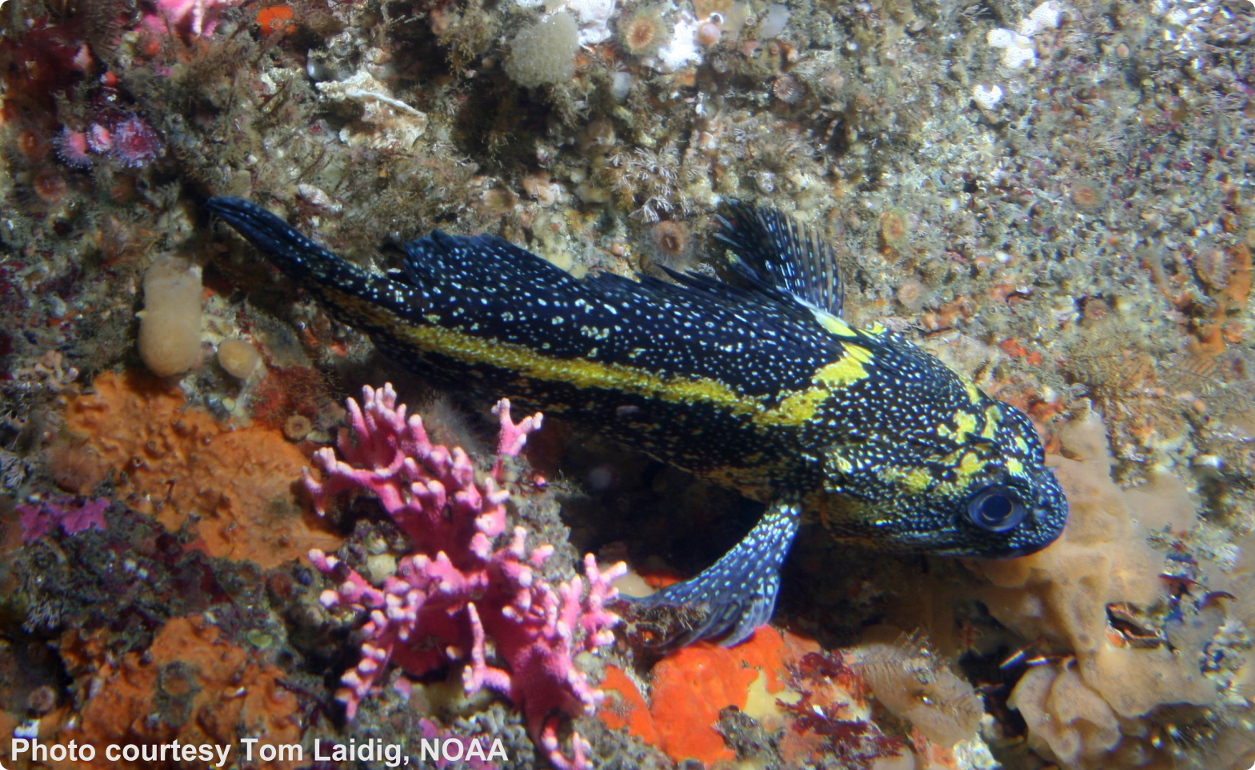
\includegraphics{cover_photo}~\\[1cm]
\pdftooltip{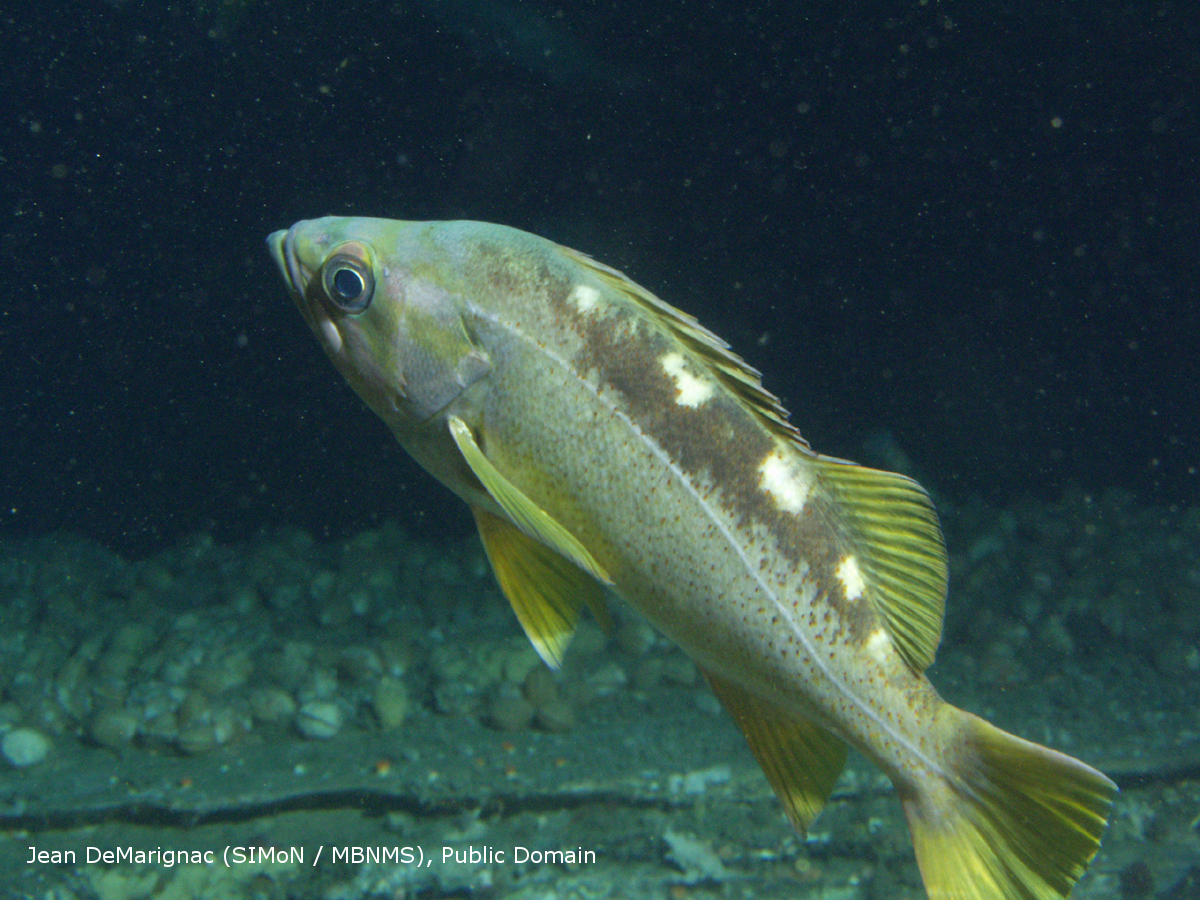
\includegraphics{Sebastes_flavidus_with_attribution}}{Yellowtail Rockfish}



Andi Stephens\textsuperscript{1}\\
Ian G. Taylor\textsuperscript{2}\\

\vspace{.5cm}

\small
\textsuperscript{1}Northwest Fisheries Science Center, U.S. Department of Commerce, National Oceanic and Atmospheric Administration, National Marine Fisheries Service, 2032 S.E. OSU Drive Newport, Oregon 97365\\

\vspace{.3cm}

\textsuperscript{2}Northwest Fisheries Science Center, U.S. Department of Commerce, National Oceanic and Atmospheric Administration, National Marine Fisheries Service, 2725 Montlake Boulevard East, Seattle, Washington 98112\\


\vspace{.5cm}

\vfill
DRAFT SAFE\\
Disclaimer: This information is distributed solely for the purpose of pre-dissemination
peer review under applicable information quality guidelines. It has not been formally
disseminated by NOAA Fisheries. It does not represent and should not be construed to
represent any agency determination or policy. 

\vspace{.3cm}
%Bottom of the page
%{\large \today}

\maketitle

\pagenumbering{roman}
\setcounter{page}{1}
\end{center}

{
\setcounter{tocdepth}{4}
\tableofcontents
}
\setlength{\parskip}{5mm plus1mm minus1mm} \pagebreak

\pagenumbering{arabic} \setcounter{page}{1}
\renewcommand{\thefigure}{\alph{figure}}
\renewcommand{\thetable}{\alph{table}}

\section*{Executive Summary}\label{executive-summary}
\addcontentsline{toc}{section}{Executive Summary}

\subsection*{Stock}\label{stock}
\addcontentsline{toc}{subsection}{Stock}

This assessment reports the status of the Yellowtail Rockfish
(\emph{Sebastes flavidus}) resource in U.S. waters off the coast of the
California, Oregon, and Washington using data through 2016.

The Pacific Fishery Management Council (PFMC) manages the U.S. fishery
as two stocks separated at Cape Mendocino, California (40\(^\circ\)
10'N). This assessment analyzes those two areas as independent stocks,
with the southern stock extending southward to the U.S./Mexico border
and the northern stock extending northward to the U.S./Canada border.

The previous assessment (Wallace and Lai
\protect\hyperlink{ref-Wallace2005}{2005}), following the pattern of
prior assessments, included only the Northern stock which it divided
into three assessment areas with divisions at Cape Elizabeth
(47\(^\circ\) 20'N) and Cape Falcon (45\(^\circ\) 46'N). However, a more
recent genetic analysis (Hess et al. n.d.) found distinct stocks north
and south of Cape Mendocino but did not find stock differences within
the northern area, with the genetic stock extending northward through
British Colombia, Canada to Southeast Alaska. However, Canada and Alaska
are not included in this assessment. Since the previous assessment,
reconstruction of historical catch by Washington and Oregon makes any
border but the state line incompatible with the data. Additionally, much
of the groundfish catch landed in northern Oregon is caught in
Washington waters.

\subsection*{Catches}\label{catches}
\addcontentsline{toc}{subsection}{Catches}

Catches from the Northern stock were divided into four categories:
commercial catch, bycatch in the at-sea hake fishery, recreational catch
in Oregon and California (north of 40\(^\circ\) 10'N), and recreational
catch in Washington. The first three of these fleets were entered in
metric tons, but the recreational catch from Washington was entered in
the model as numbers of fish with the average weight calculated
internally in the model.

Catches from the Southern stock were divided into two categories:
commercial and recreational catch, both of which were entered as metric
tons.

\hl{Include: trends and current levels-include table for last ten years and graph with 
long term data}

Catch figures: (Figures \ref{fig:r4ss_catch_N}-\ref{fig:r4ss_catch_S})\\
Catch tables: (Tables \ref{tab:Exec_catch_N}-\ref{tab:Exec_catch_S})

\FloatBarrier

\FloatBarrier

\begin{figure}[htbp]
\centering
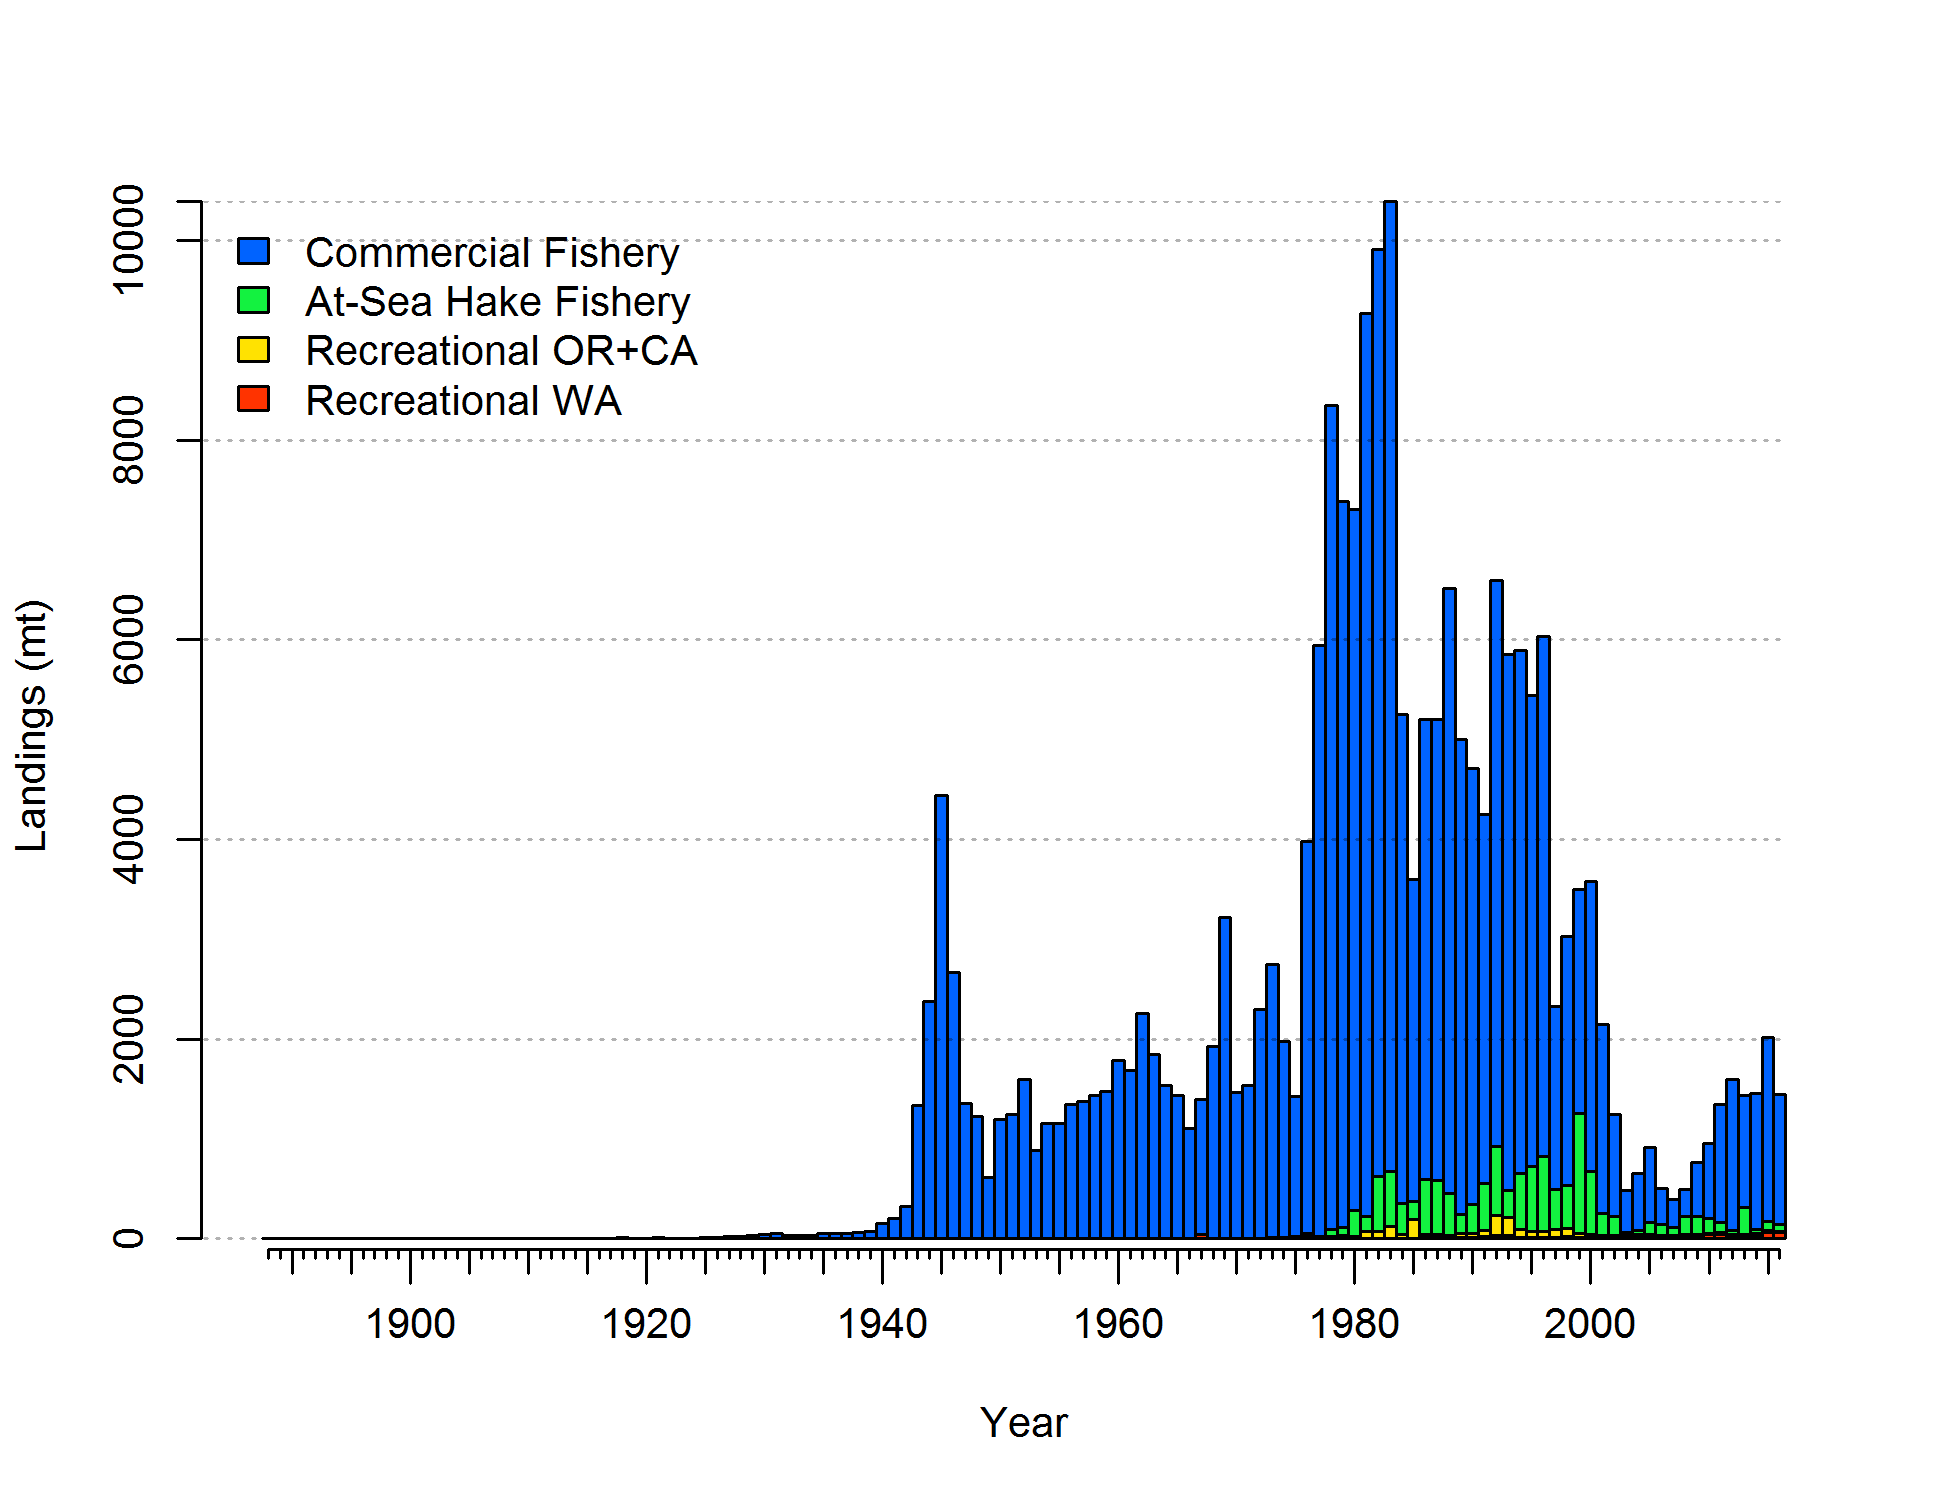
\includegraphics{r4ss/plots_mod1/catch2 landings stacked.png}
\caption{Estimated catch history of Yellowtail Rockfish in the Northern
model. Recreational catches in Washington are model estimates of total
weigth converted from input catch in numbers using model estimates of
growth and selectivity.\label{fig:r4ss_catch_N}}
\end{figure}

\begin{figure}[htbp]
\centering
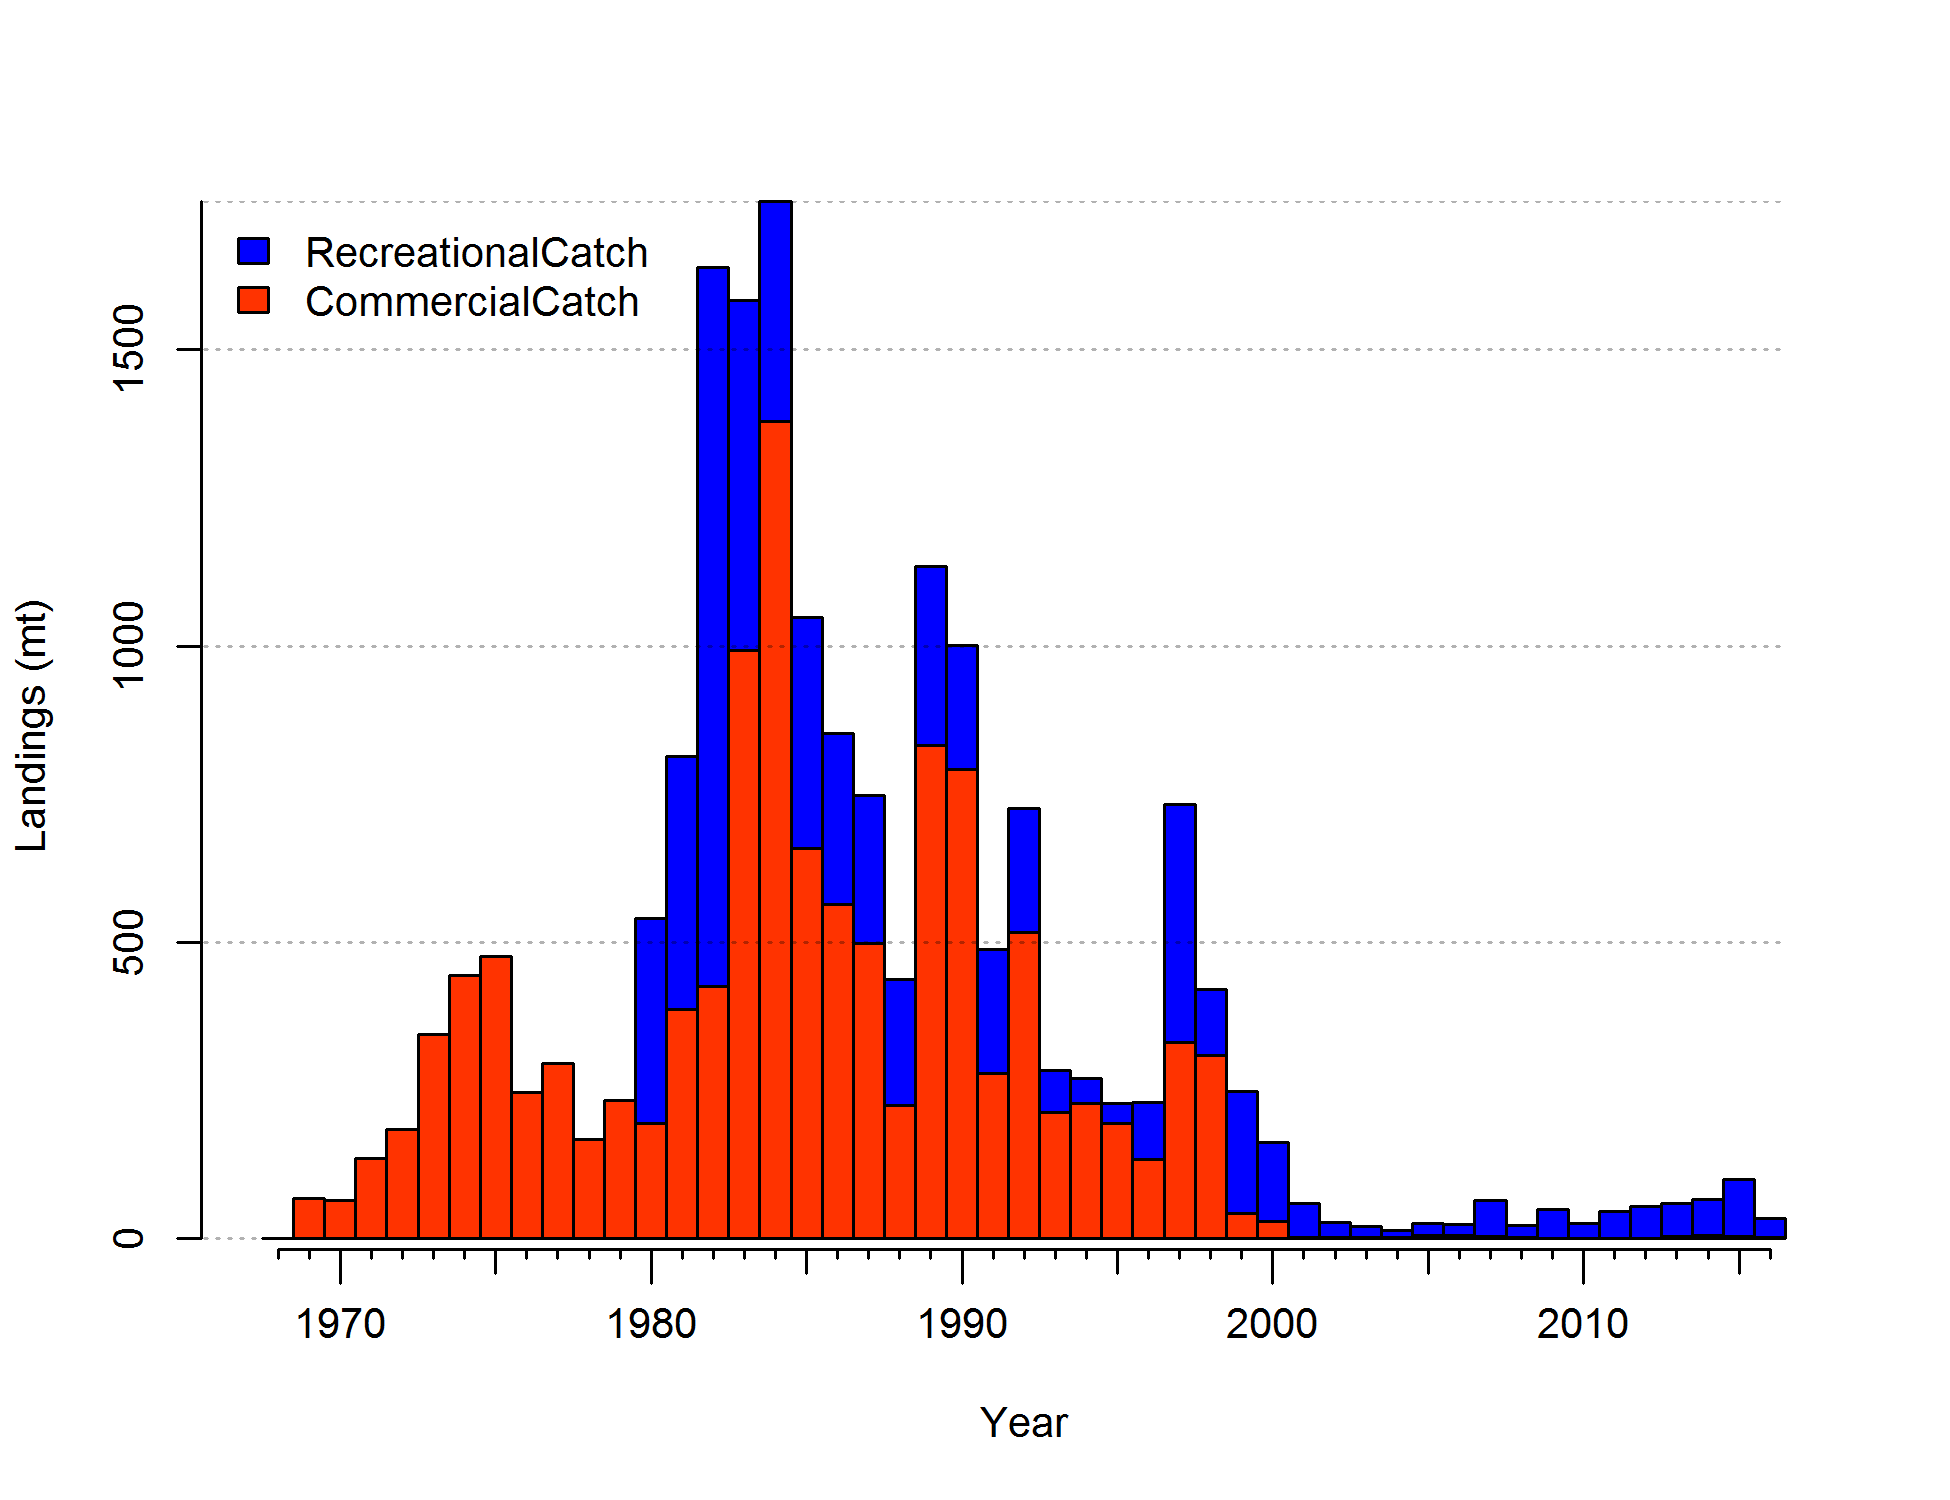
\includegraphics{r4ss/plots_mod2/catch2 landings stacked.png}
\caption{Estimated catch history of Yellowtail Rockfish in the Southern
model. \label{fig:r4ss_catch_S}}
\end{figure}

\begin{table}[ht]
\centering
\caption{Recent Yellowtail Rockfish catch by 
                                             fleet for the Northern stock 
                                             (north of 40$^\circ$ 10'N).} 
\label{tab:Exec_catch_N}
\begin{tabular}{l>{\centering}p{1.0in}>{\centering}p{1.0in}>{\centering}p{1.0in}>{\centering}p{1.0in}}
  \hline
Year & Commercial (t) & At-sea hake bycatch (t) & Recreational OR+CA (t) & Recreational WA (1000s) \\ 
  \hline
2007 & - & - & - & - \\ 
  2008 & - & - & - & - \\ 
  2009 & - & - & - & - \\ 
  2010 & - & - & - & - \\ 
  2011 & - & - & - & - \\ 
  2012 & - & - & - & - \\ 
  2013 & - & - & - & - \\ 
  2014 & - & - & - & - \\ 
  2015 & - & - & - & - \\ 
  2016 & - & - & - & - \\ 
   \hline
\end{tabular}
\end{table}

\begin{table}[ht]
\centering
\caption{Recent Yellowtail Rockfish catch by 
                                            fleet for the Southern stock 
                                             (south of 40$^\circ$ 10'N).} 
\label{tab:Exec_catch_S}
\begin{tabular}{l>{\centering}p{1.5in}>{\centering}p{1.5in}}
  \hline
Year & Recreational (t) & Commercial (t) \\ 
  \hline
2007 & - & - \\ 
  2008 & - & - \\ 
  2009 & - & - \\ 
  2010 & - & - \\ 
  2011 & - & - \\ 
  2012 & - & - \\ 
  2013 & - & - \\ 
  2014 & - & - \\ 
  2015 & - & - \\ 
  2016 & - & - \\ 
   \hline
\end{tabular}
\end{table}

\FloatBarrier

\newpage

\subsection*{Data and Assessment}\label{data-and-assessment}
\addcontentsline{toc}{subsection}{Data and Assessment}

\hl{Include: date of last assessment, type of assessment model, data available, new 
information, and information lacking.}

Yellowtail Rockfish was assessed\ldots{}. This assessment uses the
newest version of Stock Synthesis (3.xxx). The model begins in 1889, and
assumes the stock was at an unfished equilibrium that year.

Map of assessment region: (Figure \ref{fig:assess_region_map}).

\begin{figure}[htbp]
\centering
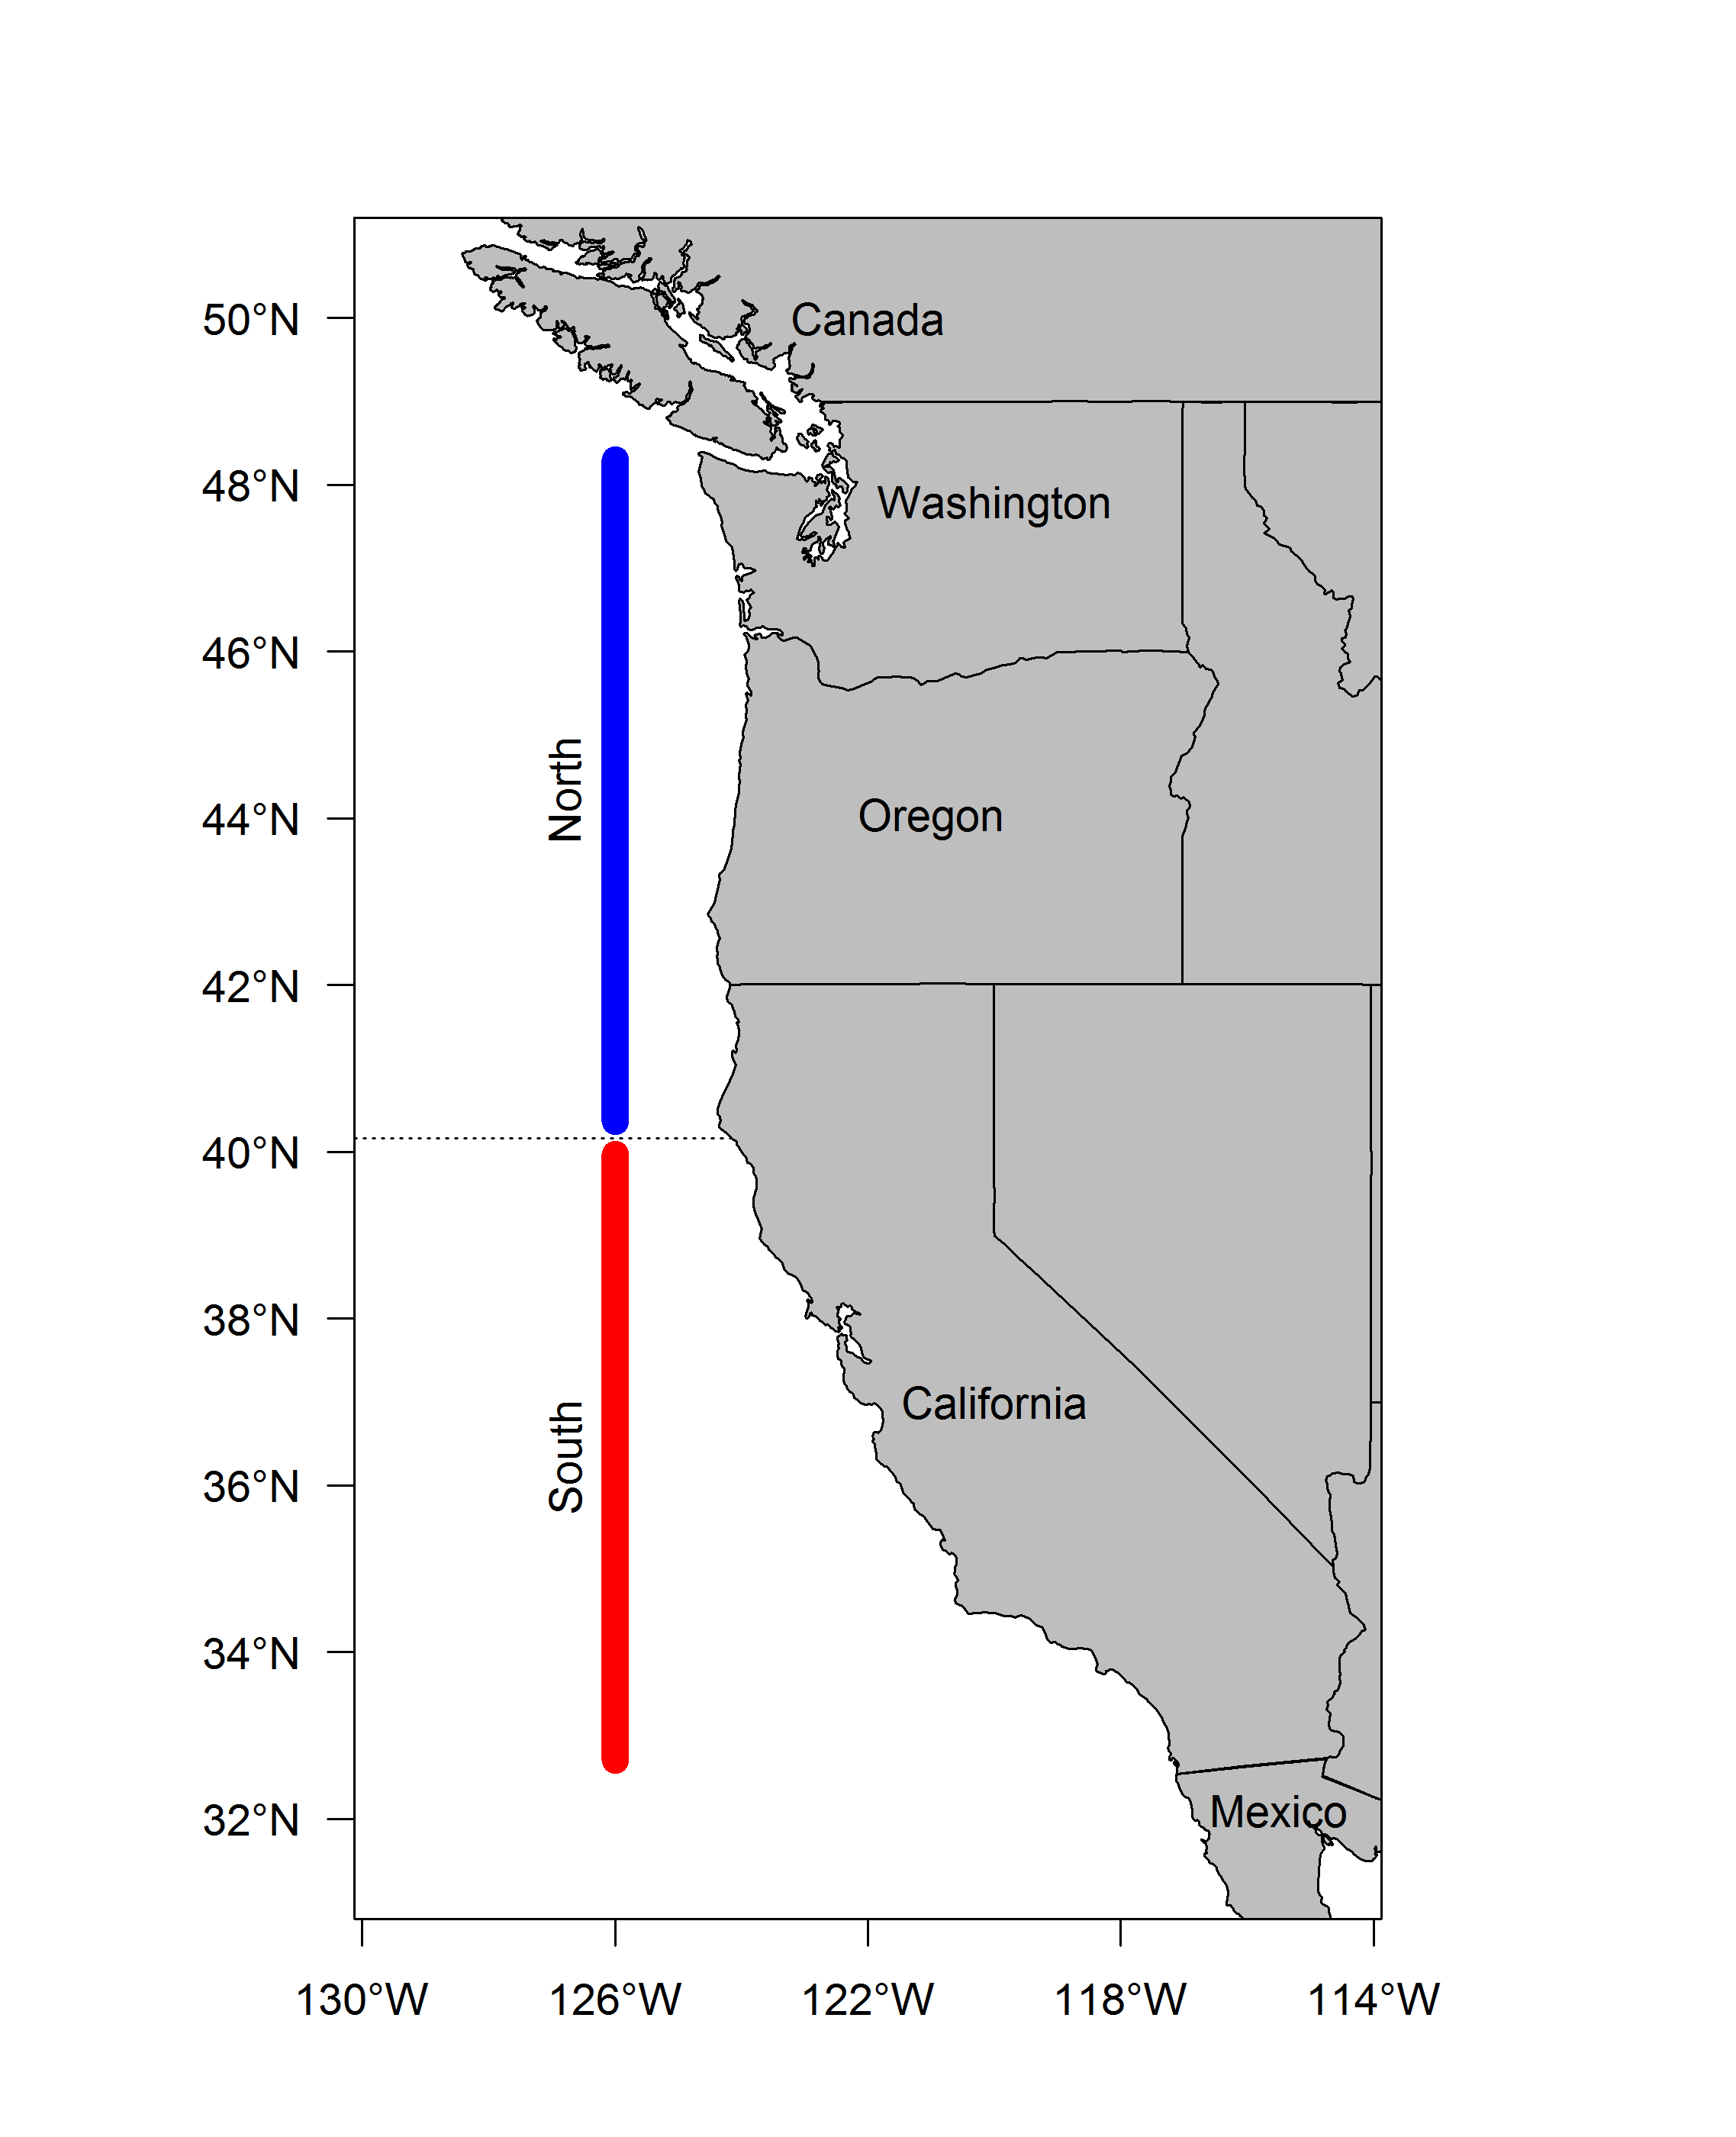
\includegraphics{Figures/assess_region_map.png}
\caption{Map depicting the boundaries for the base-case model.
\label{fig:assess_region_map}}
\end{figure}

\FloatBarrier

\subsection*{Stock Biomass}\label{stock-biomass}
\addcontentsline{toc}{subsection}{Stock Biomass}

\hl{Include: trends and current levels relative to virgin or historic levels, 
description of uncertainty-include table for last 10 years and graph with 
long term estimates.}

Spawning output Figure: Figure \ref{fig:Spawnbio_all}\\
Spawning output Table(s): Table \ref{tab:SpawningDeplete_mod1}\\
Relative depletion Figure: Figure \ref{fig:RelDeplete_all}

Example text (remove Models 2 and 3 if not needed - if using, remove the
\# in-line comments!!!)\\
The estimated relative depletion level (spawning output relative to
unfished spawning output) of the the base-case model in 2016 is 53\%
(\textasciitilde{}95\% asymptotic interval: \(\pm\) 41.3\%-64.8\%)
(Figure \ref{fig:RelDeplete_all}).

The estimated relative depletion level of model 2 in 2016 is 92.2\%
(\textasciitilde{}95\% asymptotic interval: \(\pm\) 72.1\%-112\%)
(Figure \ref{fig:RelDeplete_all}).

The estimated relative depletion level of model 3 in 2016 is
(\textasciitilde{}95\% asymptotic interval: \(\pm\) ) (Figure
\ref{fig:RelDeplete_all}).

\FloatBarrier

\begin{table}[ht]
\centering
\caption{Recent trend in beginning of the 
                                      year spawning output and depletion for
                                      the Northern model for Yellowtail Rockfish.} 
\label{tab:SpawningDeplete_mod1}
\begin{tabular}{l>{\centering}p{1.3in}>{\centering}p{1.2in}>{\centering}p{1in}>{\centering}p{1.2in}}
  \hline
Year & Spawning Output (trillion eggs) & \~{} 95\% confidence interval & Estimated depletion & \~{} 95\% confidence interval \\ 
  \hline
2008 & 7.307 & (5.31-9.3) & 0.497 & (0.368-0.627) \\ 
  2009 & 7.713 & (5.65-9.78) & 0.525 & (0.394-0.656) \\ 
  2010 & 7.991 & (5.87-10.12) & 0.544 & (0.412-0.676) \\ 
  2011 & 8.105 & (5.94-10.27) & 0.552 & (0.42-0.683) \\ 
  2012 & 8.160 & (5.98-10.34) & 0.555 & (0.426-0.685) \\ 
  2013 & 8.101 & (5.91-10.29) & 0.551 & (0.425-0.677) \\ 
  2014 & 8.021 & (5.83-10.21) & 0.546 & (0.423-0.669) \\ 
  2015 & 7.943 & (5.75-10.14) & 0.541 & (0.421-0.661) \\ 
  2016 & 7.806 & (5.6-10.02) & 0.531 & (0.413-0.65) \\ 
  2017 & 7.791 & (5.55-10.03) & 0.530 & (0.413-0.648) \\ 
   \hline
\end{tabular}
\end{table}\begin{table}[ht]
\centering
\caption{Recent trend in 
                                             beginning of the year spawning output
                                             and depletion for the Southern model for Yellowtail Rockfish.} 
\label{tab:SpawningDeplete_mod2}
\begin{tabular}{l>{\centering}p{1.3in}>{\centering}p{1.2in}>{\centering}p{1in}>{\centering}p{1.2in}}
  \hline
Year & Spawning Output (trillion eggs) & \~{} 95\% confidence interval & Estimated depletion & \~{} 95\% confidence interval \\ 
  \hline
2008 & 1.983 & (-0.76-4.72) & 0.588 & (0.45-0.726) \\ 
  2009 & 1.975 & (-0.74-4.69) & 0.586 & (0.453-0.718) \\ 
  2010 & 1.989 & (-0.73-4.71) & 0.590 & (0.461-0.719) \\ 
  2011 & 2.027 & (-0.73-4.78) & 0.601 & (0.473-0.729) \\ 
  2012 & 2.084 & (-0.73-4.9) & 0.618 & (0.489-0.747) \\ 
  2013 & 2.177 & (-0.75-5.11) & 0.646 & (0.512-0.779) \\ 
  2014 & 2.298 & (-0.78-5.38) & 0.682 & (0.543-0.821) \\ 
  2015 & 2.478 & (-0.83-5.79) & 0.735 & (0.584-0.886) \\ 
  2016 & 2.743 & (-0.91-6.39) & 0.814 & (0.643-0.984) \\ 
  2017 & 3.109 & (-1.02-7.23) & 0.922 & (0.721-1.123) \\ 
   \hline
\end{tabular}
\end{table}

\FloatBarrier

\begin{figure}[htbp]
\centering
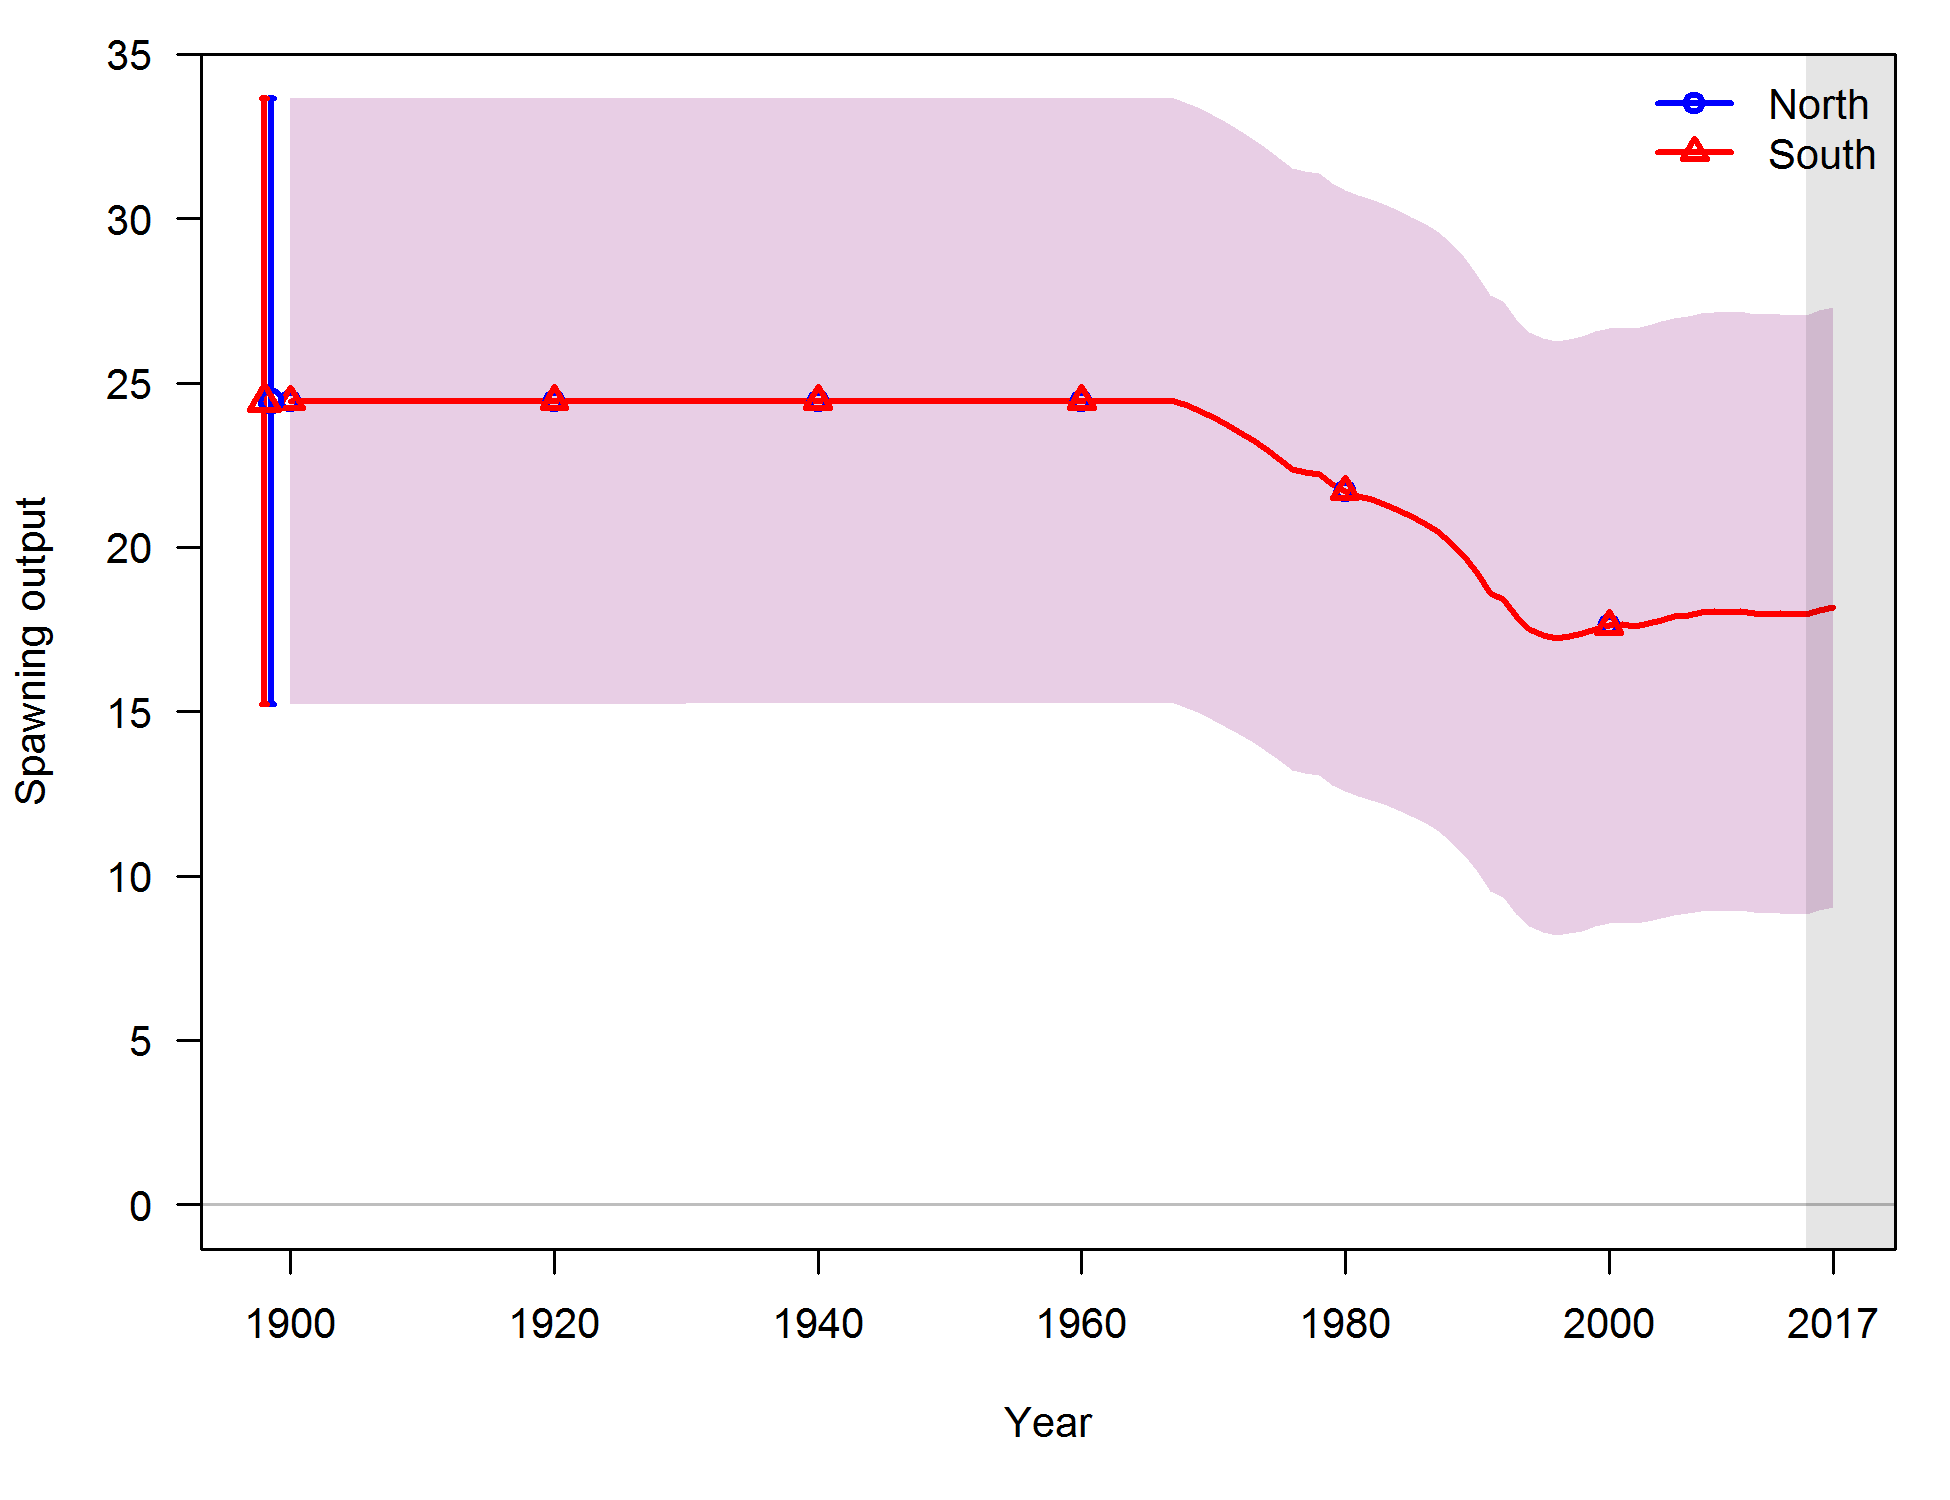
\includegraphics{r4ss/plots_compare/base_compare2_spawnbio_uncertainty.png}
\caption{Time series of spawning output trajectory (circles and line:
median; light broken lines: 95\% credibility intervals) for the base
case assessment model. \label{fig:Spawnbio_all}}
\end{figure}

\begin{figure}[htbp]
\centering
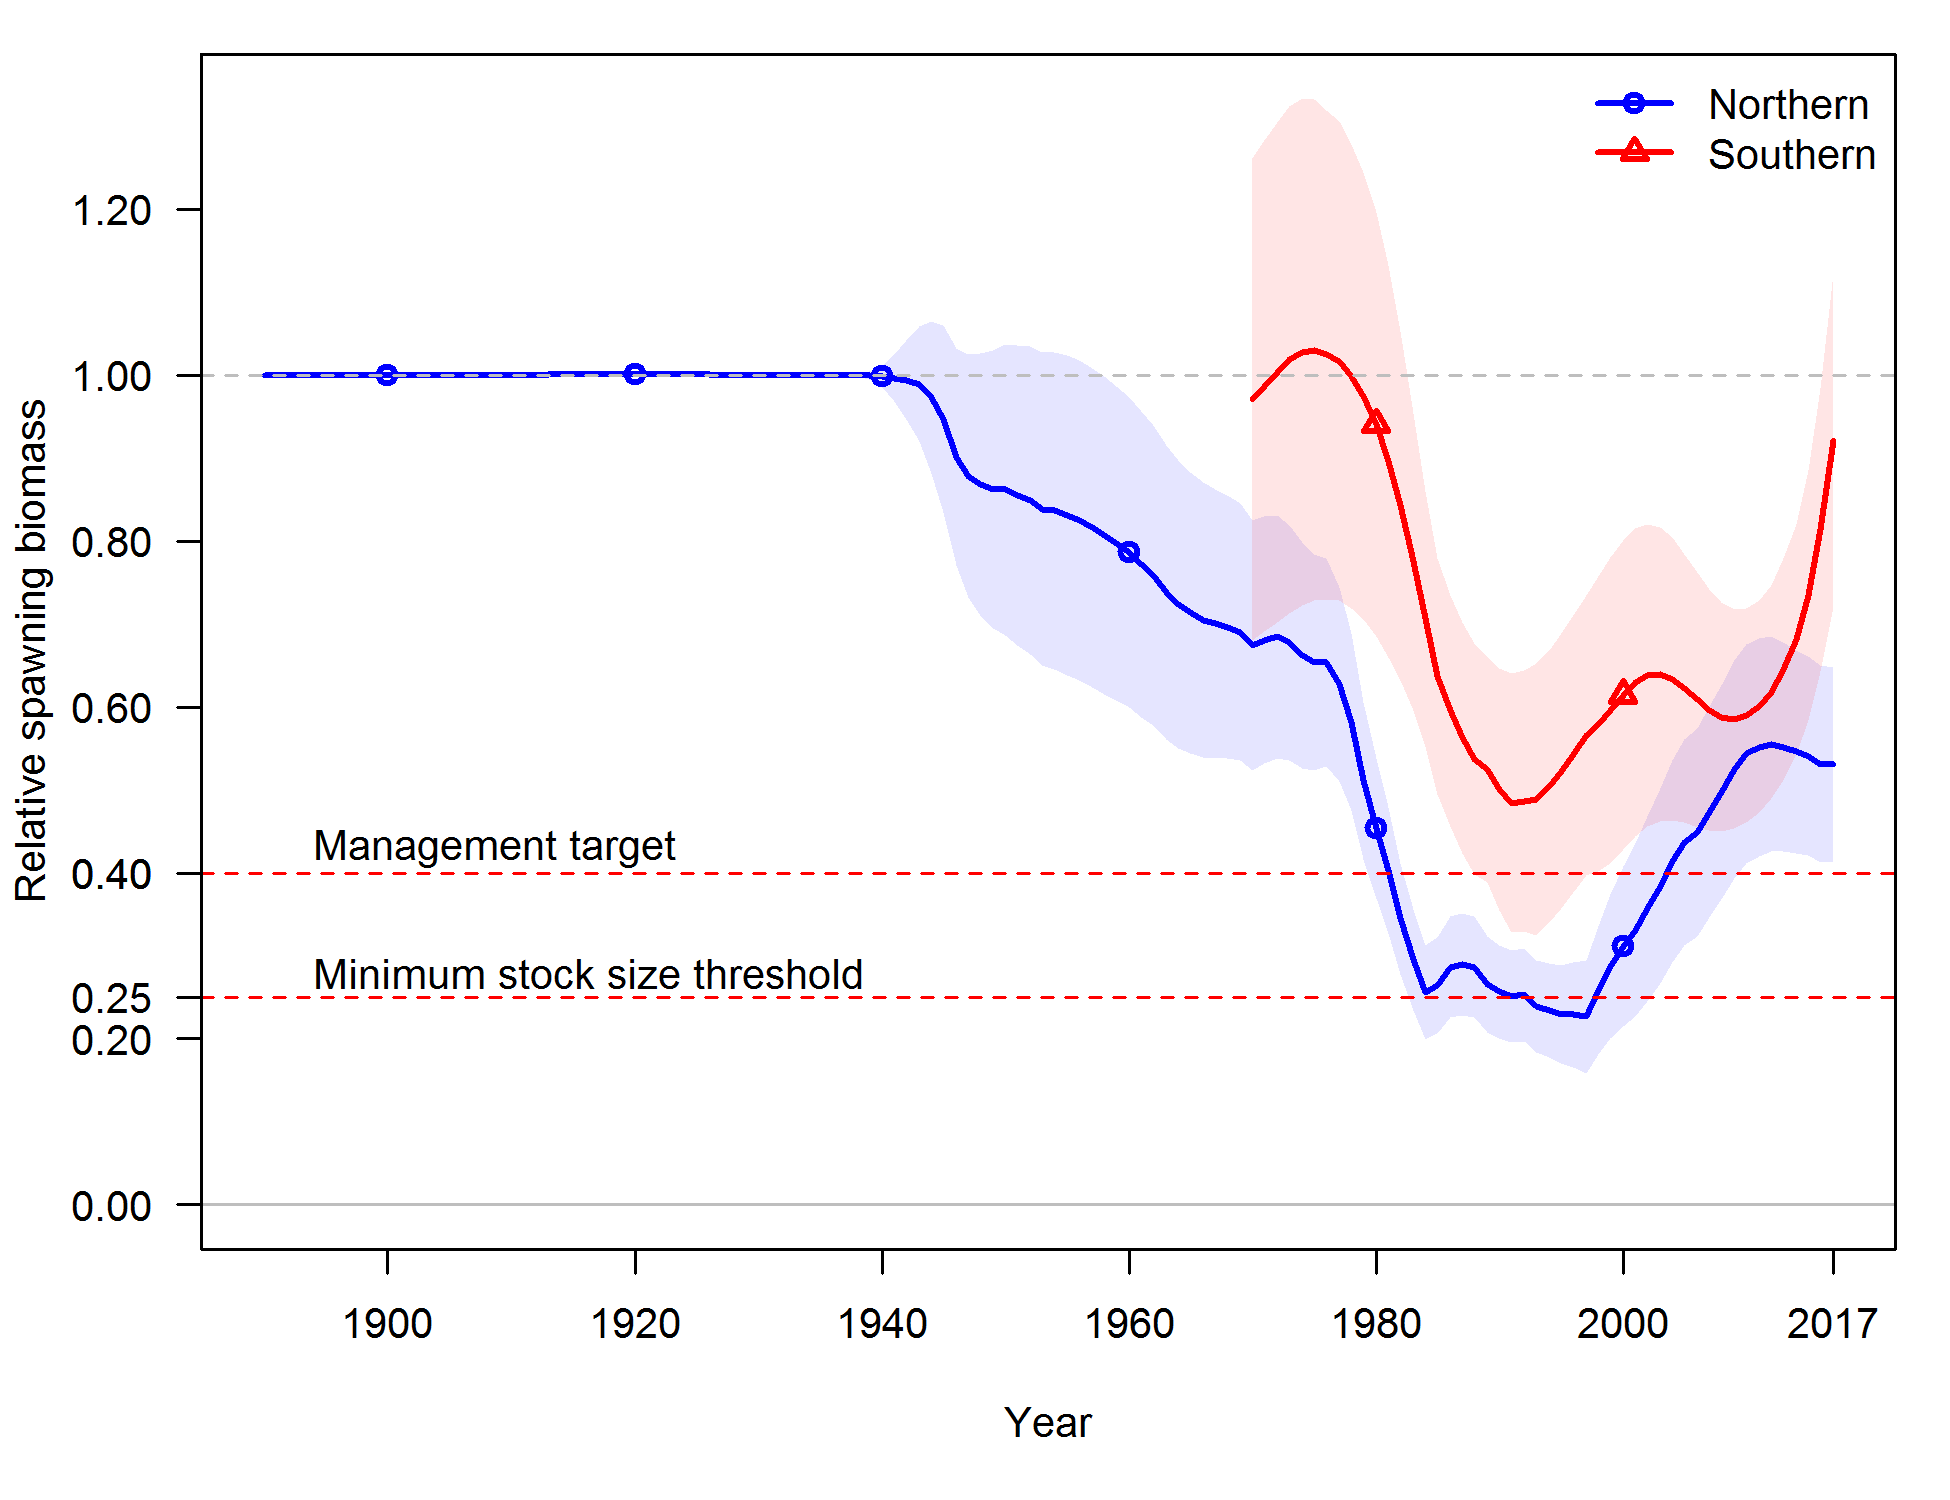
\includegraphics{r4ss/plots_compare/base_compare4_Bratio_uncertainty.png}
\caption{Estimated relative depletion with approximate 95\% asymptotic
confidnce intervals (dashed lines) for the base case assessment model.
\label{fig:RelDeplete_all}}
\end{figure}

\FloatBarrier

\subsection*{Recruitment}\label{recruitment}
\addcontentsline{toc}{subsection}{Recruitment}

\hl{Include: trends and current levels relative to virgin or historic levels-include 
table for last 10 years and graph with long term estimates.}

Recruitment Figure: (Figure \ref{fig:Recruits_all})\\
Recruitment Tables: (Tables \ref{tab:Recruit_mod1},
\ref{tab:Recruit_mod2} and \ref{tab:Recruit_mod3})

\begin{table}[ht]
\centering
\caption{Recent recruitment for the Northern model.} 
\label{tab:Recruit_mod1}
\begin{tabular}{>{\centering}p{.8in}>{\centering}p{1.6in}>{\centering}p{1.3in}}
  \hline
Year & Estimated Recruitment (millions) & \~{} 95\% confidence interval \\ 
  \hline
2008 & 34.46 & (20.8 - 57.08) \\ 
  2009 & 10.44 & (5.04 - 21.65) \\ 
  2010 & 22.11 & (11.8 - 41.43) \\ 
  2011 & 15.15 & (6.89 - 33.31) \\ 
  2012 & 15.95 & (6.29 - 40.42) \\ 
  2013 & 25.87 & (8.87 - 75.43) \\ 
  2014 & 24.05 & (8.24 - 70.21) \\ 
  2015 & 24.51 & (8.62 - 69.71) \\ 
  2016 & 24.35 & (8.57 - 69.16) \\ 
  2017 & 24.34 & (8.57 - 69.13) \\ 
   \hline
\end{tabular}
\end{table}\begin{table}[ht]
\centering
\caption{Recent recruitment for the Southern model.} 
\label{tab:Recruit_mod2}
\begin{tabular}{>{\centering}p{.8in}>{\centering}p{1.6in}>{\centering}p{1.3in}}
  \hline
Year & Estimated Recruitment (millions) & \~{} 95\% confidence interval \\ 
  \hline
2008 & 123.60 & (31.9 - 478.95) \\ 
  2009 & 61.44 & (9.88 - 382.1) \\ 
  2010 & 84.06 & (14.63 - 483.13) \\ 
  2011 & 68.11 & (12.28 - 377.66) \\ 
  2012 & 35.52 & (6.07 - 207.89) \\ 
  2013 & 41.50 & (8.35 - 206.26) \\ 
  2014 & 32.55 & (6.23 - 170.09) \\ 
  2015 & 25.26 & (4.87 - 131.01) \\ 
  2016 & 21.17 & (3.94 - 113.89) \\ 
  2017 & 21.81 & (4.06 - 117.31) \\ 
   \hline
\end{tabular}
\end{table}

\FloatBarrier

\begin{figure}[htbp]
\centering
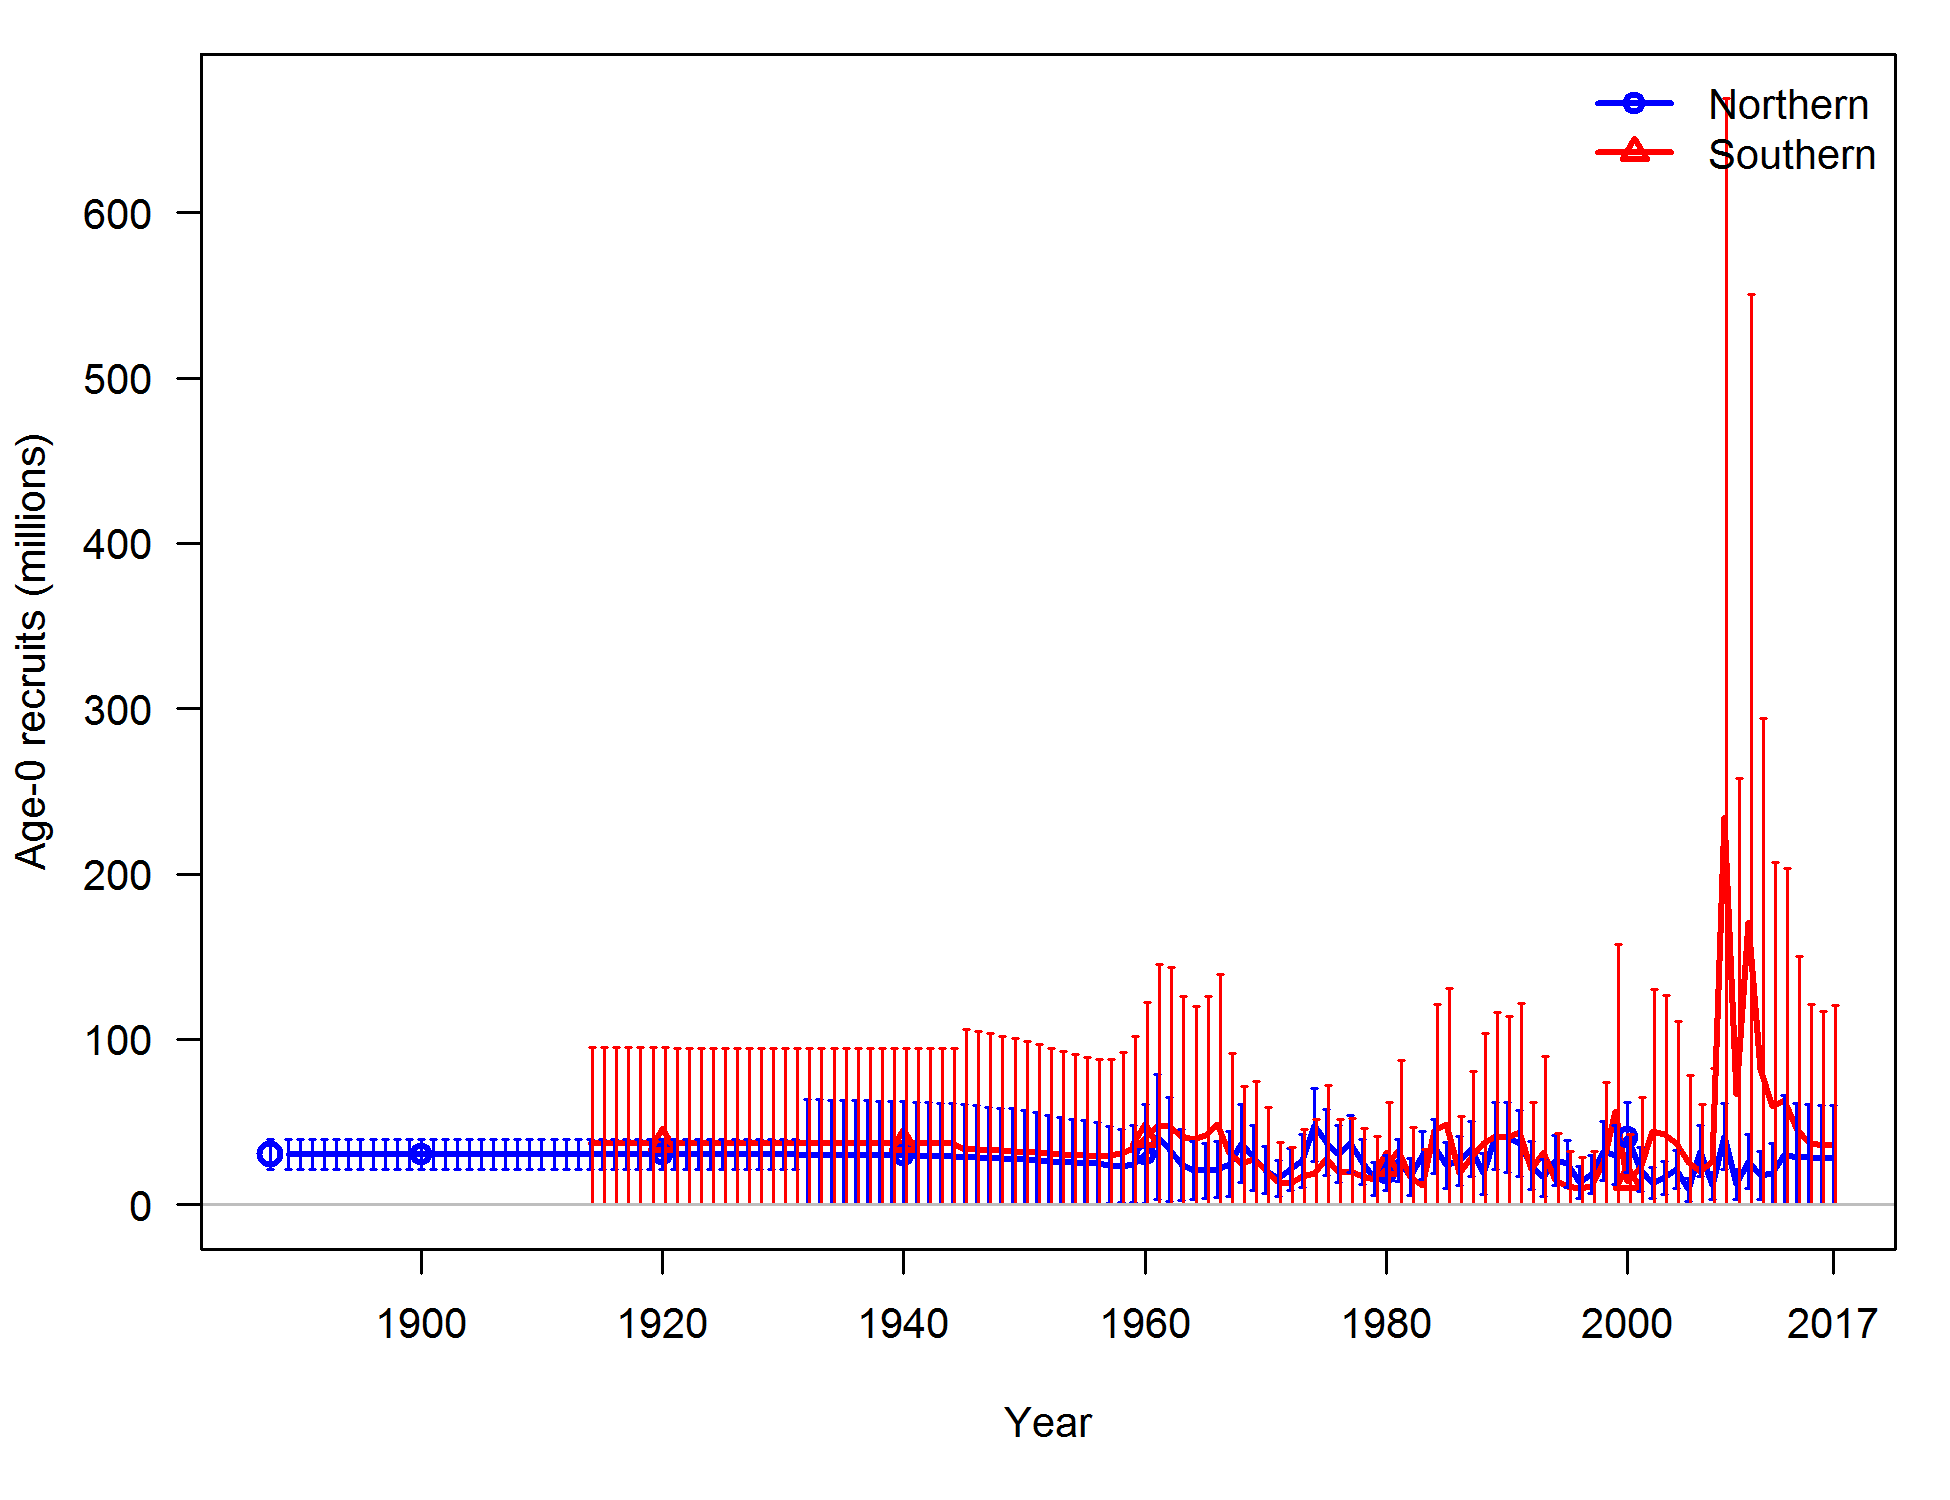
\includegraphics{r4ss/plots_compare/base_compare8_recruits_uncertainty.png}
\caption{Time series of estimated Yellowtail Rockfish recruitments for
the base-case model with 95\% confidence or credibility intervals.
\label{fig:Recruits_all}}
\end{figure}

\FloatBarrier

\subsection*{Exploitation status}\label{exploitation-status}
\addcontentsline{toc}{subsection}{Exploitation status}

\hl{Include: exploitation rates (i.e., total catch divided by exploitable biomass, or the annual SPR harvest rate) – include a table with the last 10 years of data and a graph showing the trend in fishing mortality relative to the target (y-axis) plotted against the trend in biomass relative to the target (x-axis).}

Exploitation Tables: Table \ref{tab:SPR_Exploit_mod1}, Table
\ref{tab:SPR_Exploit_mod2}, Table \ref{tab:SPR_Exploit_mod3}
Exploitation Figure: Figure \ref{fig:SPR_all}).

A summary of Yellowtail Rockfish exploitation histories for base model
is provided as Figure \ref{fig:Phase_all}.

\FloatBarrier

\begin{table}[ht]
\centering
\caption{Recent trend in spawning potential 
                                        ratio and exploitation for Yellowtail Rockfish in the Northern model.  Fishing intensity is (1-SPR) 
                                        divided by 50\% (the SPR target) and exploitation 
                                        is F divided by F\textsubscript{SPR}.} 
\label{tab:SPR_Exploit_mod1}
\begin{tabular}{l>{\centering}p{1in}>{\centering}p{1.2in}>{\centering}p{1in}>{\centering}p{1.2in}}
  \hline
Year & Fishing intensity & \~{} 95\% confidence interval & Exploitation rate & \~{} 95\% confidence interval \\ 
  \hline
2007 & 0.33 & (0.12-0.55) & 0.01 & (0-0.02) \\ 
  2008 & 0.21 & (0.14-0.28) & 0.01 & (0-0.01) \\ 
  2009 & 0.39 & (0.24-0.54) & 0.01 & (0.01-0.02) \\ 
  2010 & 0.52 & (0.27-0.77) & 0.02 & (0.01-0.03) \\ 
  2011 & 0.45 & (0.33-0.58) & 0.02 & (0.01-0.02) \\ 
  2012 & 0.52 & (0.38-0.65) & 0.02 & (0.01-0.03) \\ 
  2013 & 0.49 & (0.36-0.62) & 0.02 & (0.01-0.02) \\ 
  2014 & 0.49 & (0.36-0.62) & 0.02 & (0.01-0.02) \\ 
  2015 & 0.63 & (0.48-0.79) & 0.03 & (0.02-0.03) \\ 
  2016 & 0.50 & (0.36-0.63) & 0.02 & (0.01-0.02) \\ 
   \hline
\end{tabular}
\end{table}\begin{table}[ht]
\centering
\caption{Recent trend in spawning potential 
                                        ratio and exploitation for Yellowtail Rockfish in the Southern model. Fishing intensity is (1-SPR) 
                                        divided by 50\% (the SPR target) and exploitation 
                                        is F divided by F\textsubscript{SPR}.} 
\label{tab:SPR_Exploit_mod2}
\begin{tabular}{l>{\centering}p{1in}>{\centering}p{1.2in}>{\centering}p{1in}>{\centering}p{1.2in}}
  \hline
Year & Fishing intensity & \~{} 95\% confidence interval & Exploitation rate & \~{} 95\% confidence interval \\ 
  \hline
2007 & 0.04 & (-0.01-0.1) & 0.00 & (0-0) \\ 
  2008 & 0.02 & (0-0.04) & 0.00 & (0-0) \\ 
  2009 & 0.03 & (-0.01-0.07) & 0.00 & (0-0) \\ 
  2010 & 0.01 & (0-0.03) & 0.00 & (0-0) \\ 
  2011 & 0.02 & (-0.01-0.05) & 0.00 & (0-0) \\ 
  2012 & 0.02 & (-0.01-0.05) & 0.00 & (0-0) \\ 
  2013 & 0.02 & (-0.01-0.05) & 0.00 & (0-0) \\ 
  2014 & 0.02 & (-0.01-0.05) & 0.00 & (0-0) \\ 
  2015 & 0.03 & (-0.01-0.07) & 0.00 & (0-0) \\ 
  2016 & 0.01 & (0-0.02) & 0.00 & (0-0) \\ 
   \hline
\end{tabular}
\end{table}

\FloatBarrier

\begin{figure}[htbp]
\centering
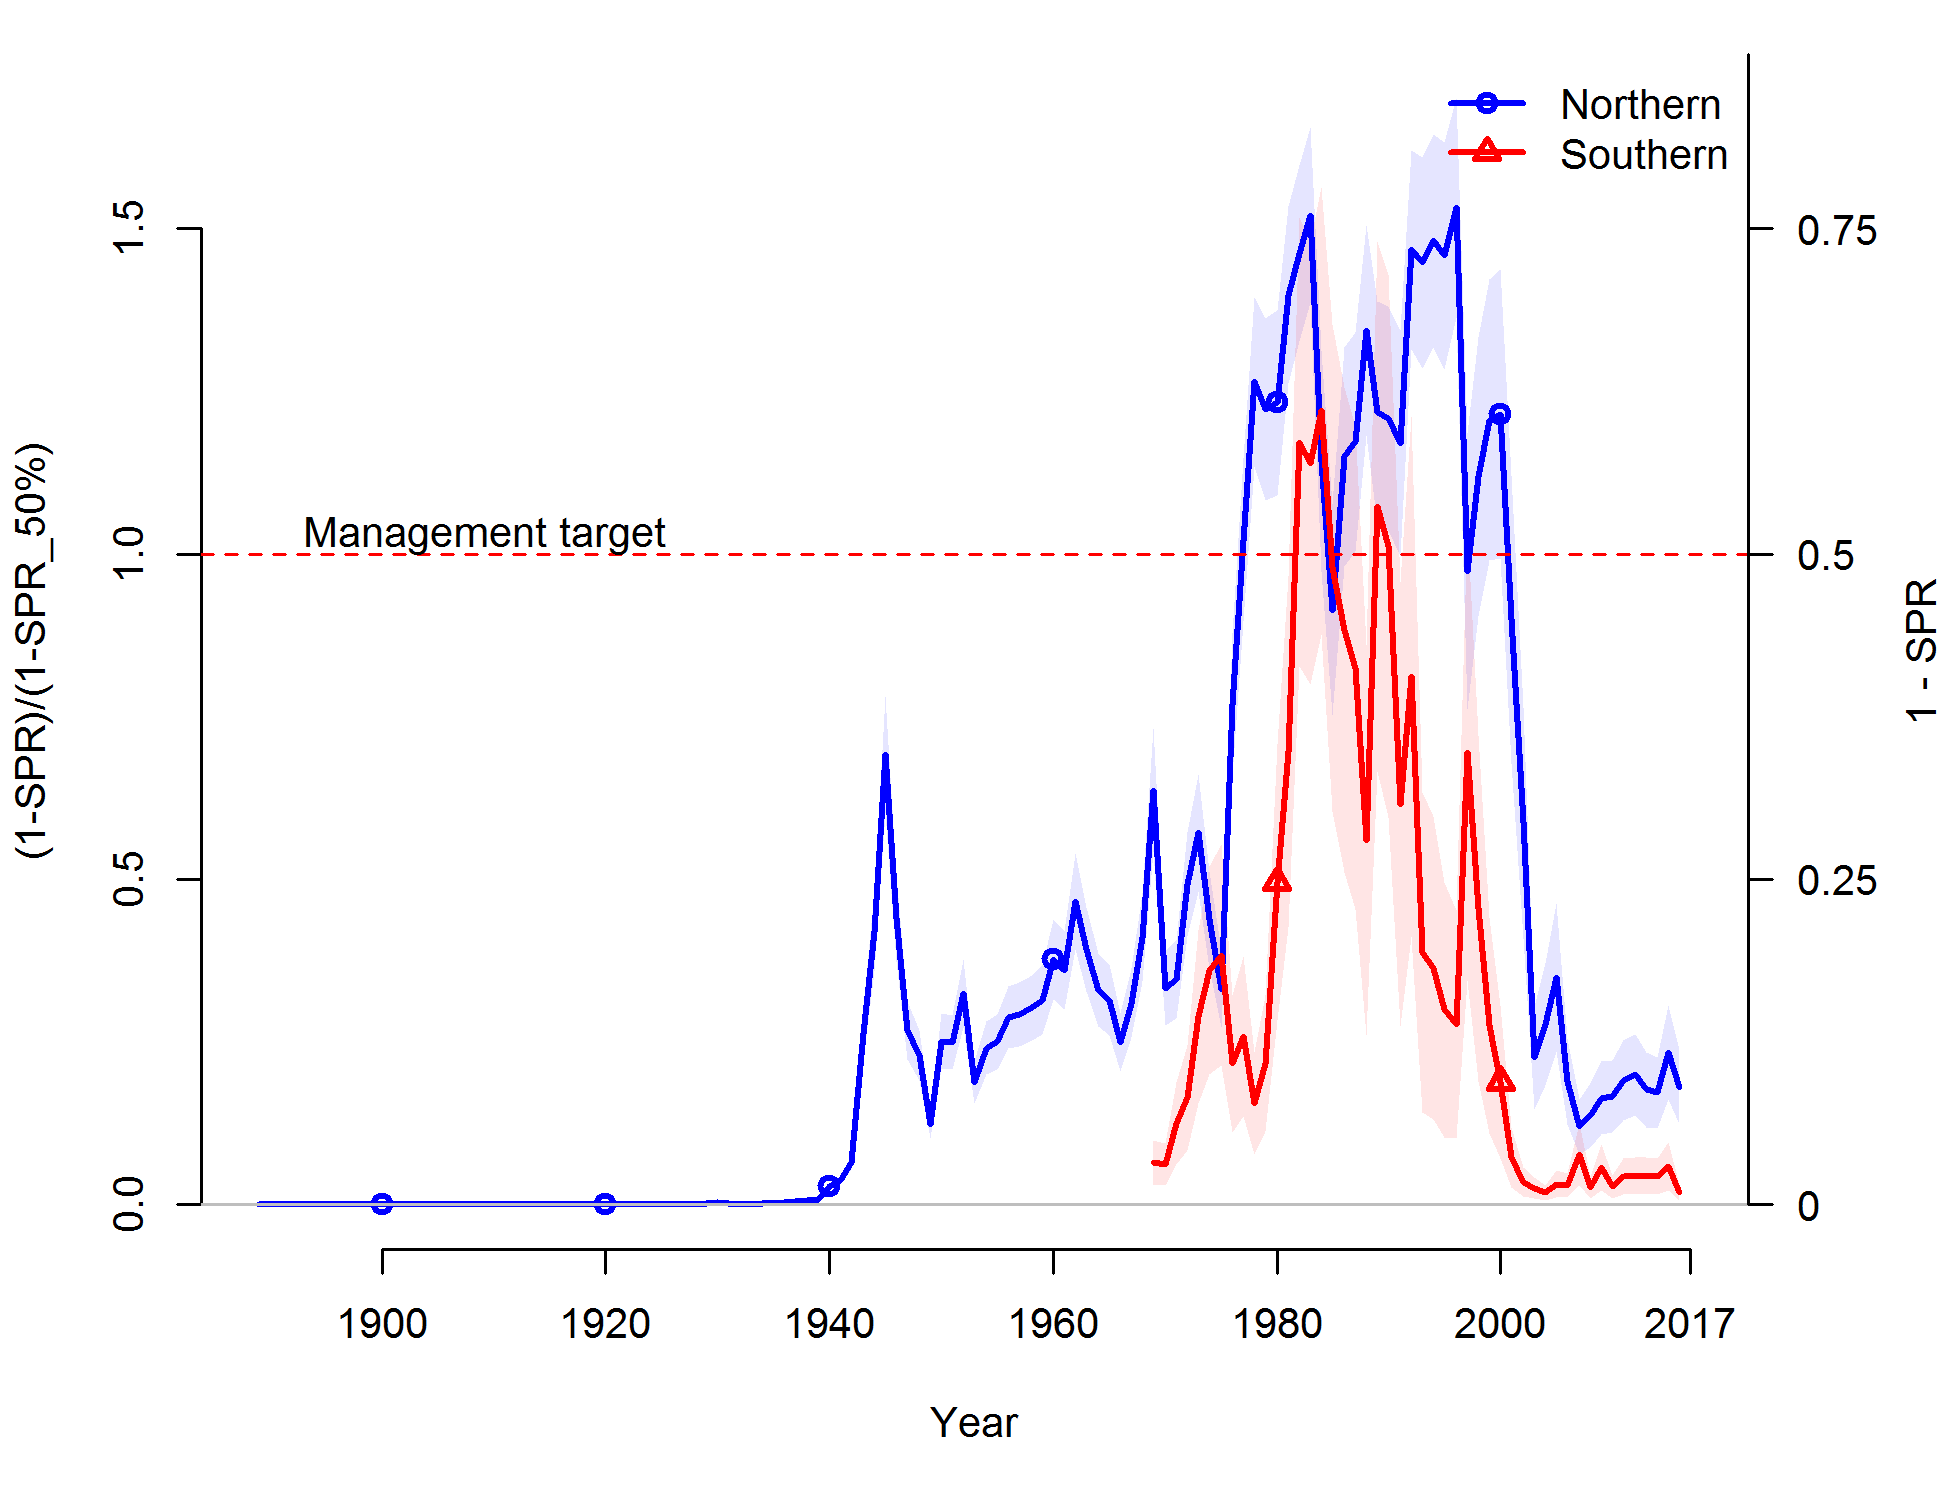
\includegraphics{r4ss/plots_compare/base_compare6_SPRratio_uncertainty.png}
\caption{Estimated spawning potential ratio (SPR) for the base-case
model. One minus SPR is plotted so that higher exploitation rates occur
on the upper portion of the y-axis. The management target is plotted as
a red horizontal line and values above this reflect harvests in excess
of the overfishing proxy based on the SPR\textsubscript{50\%} harvest
rate. The last year in the time series is 2016. \label{fig:SPR_all}}
\end{figure}

\begin{figure}[htbp]
\centering
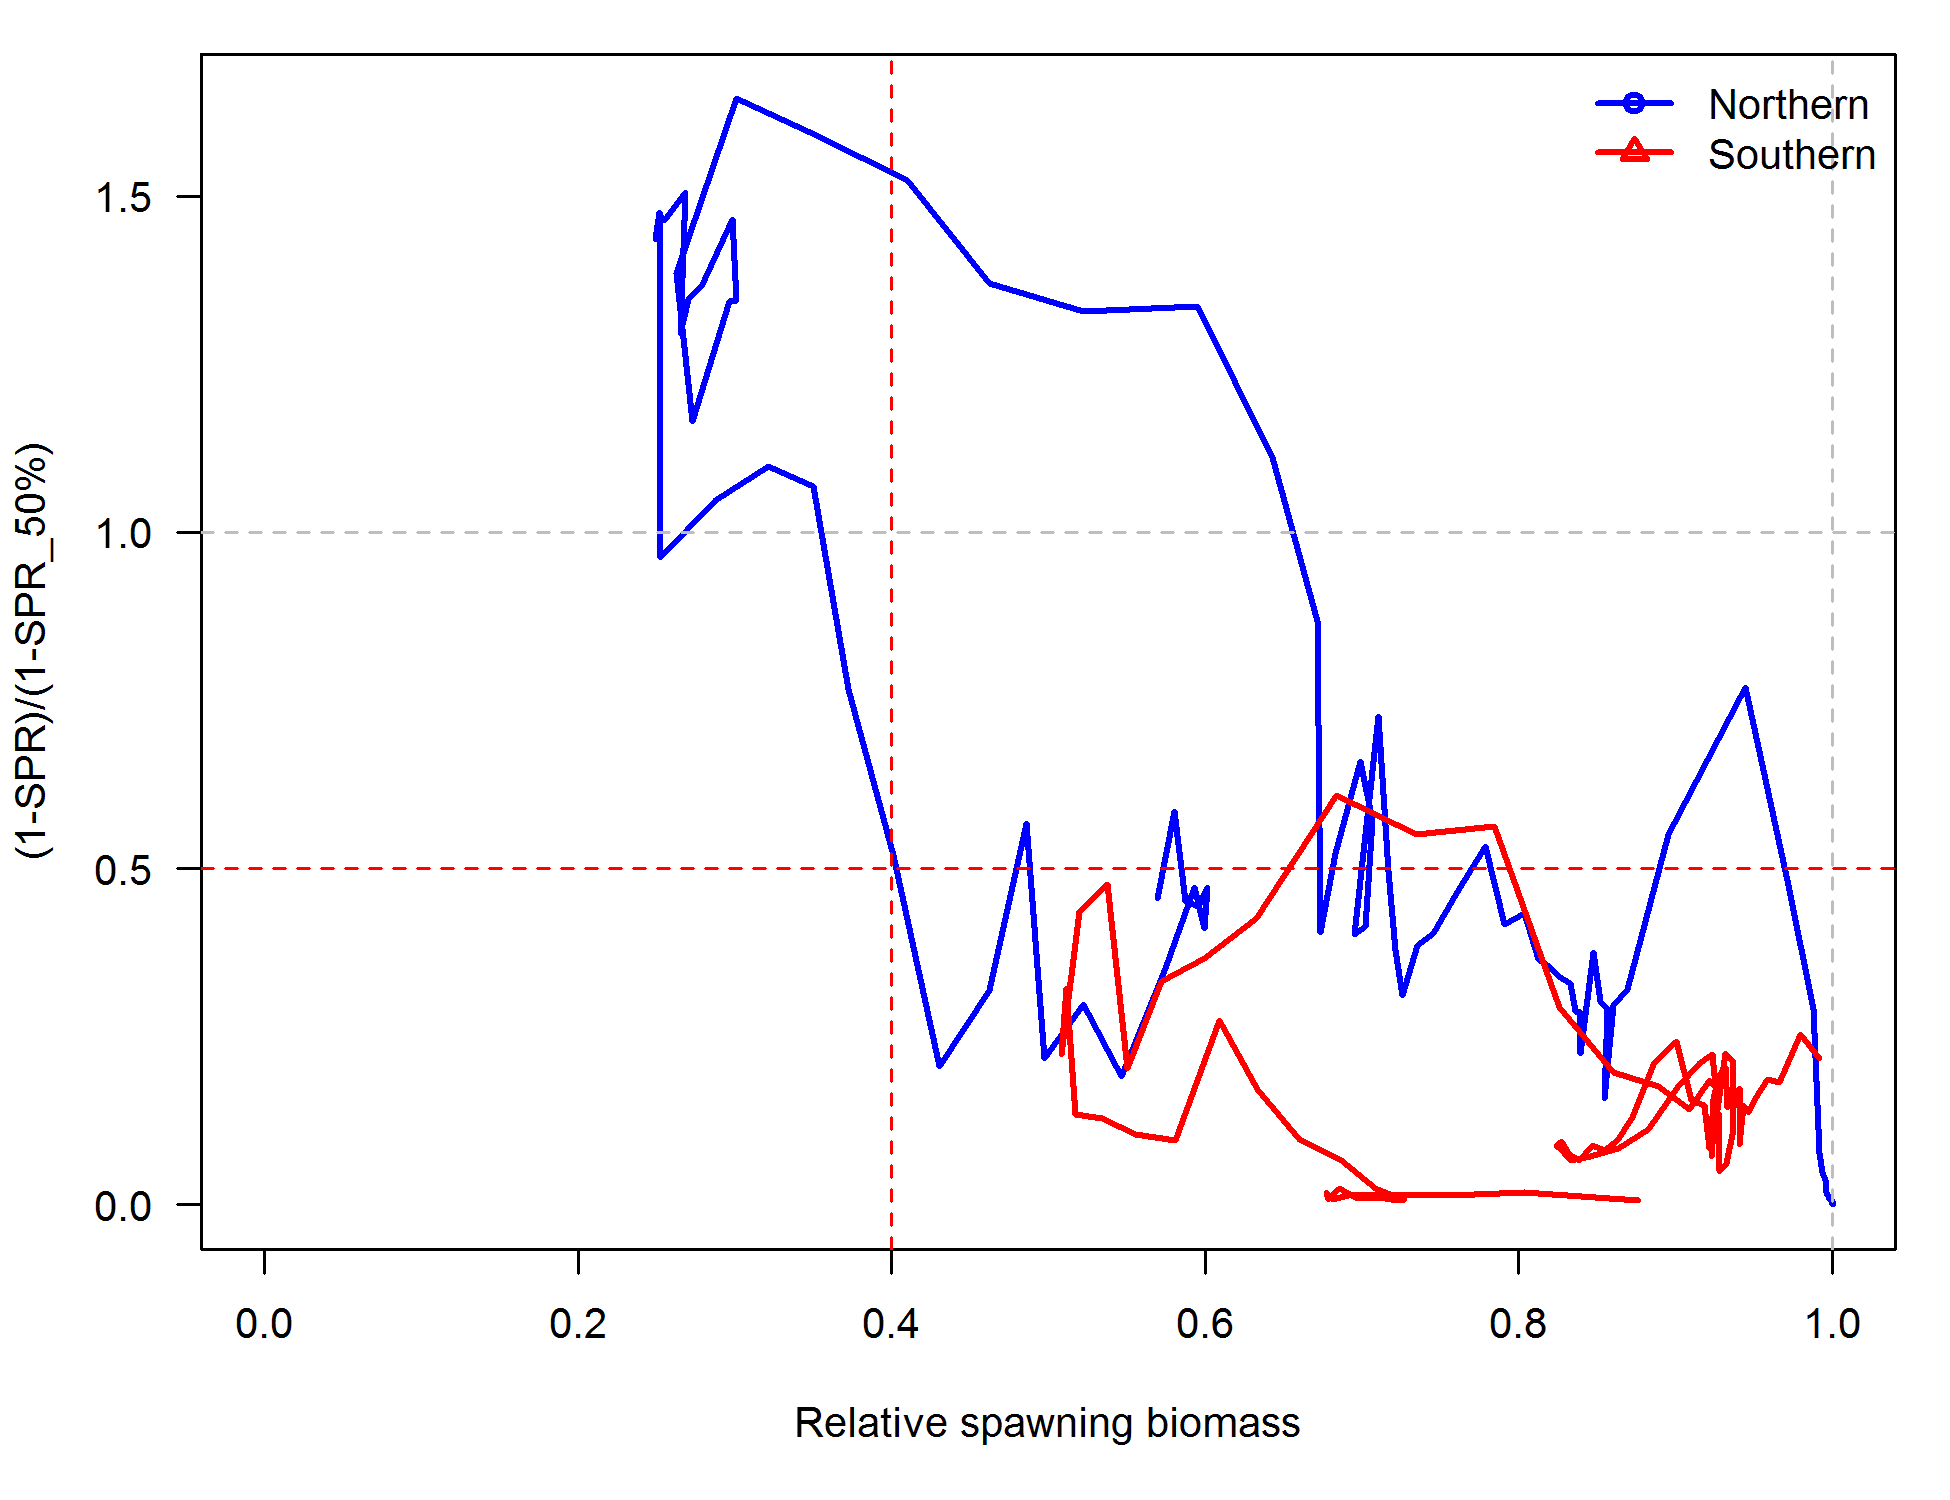
\includegraphics{r4ss/plots_compare/base_compare13_phase_plot.png}
\caption{Phase plot of estimated relative (1-SPR) vs.~relative spawning
biomass for the base case model. The relative (1-SPR) is (1-SPR) divided
by 50\% (the SPR target). Relative depletion is the annual spawning
biomass divided by the unfished spawning biomass. \label{fig:Phase_all}}
\end{figure}

\FloatBarrier

\subsection*{Ecosystem Considerations}\label{ecosystem-considerations}
\addcontentsline{toc}{subsection}{Ecosystem Considerations}

In this assessment, ecosystem considerations were\ldots{}..

\subsection*{Reference Points}\label{reference-points}
\addcontentsline{toc}{subsection}{Reference Points}

\hl{Include:} management targets and definition of overfishing,
including the harvest rate that brings the stock to equilibrium at
\(B_{40\%}\) (the \(B_{MSY}\) proxy) and the equilibrium stock size that
results from fishing at the default harvest rate (the \(F_{MSY}\)
proxy). Include a summary table that compares estimated reference points
for SSB, SPR, Exploitation Rate and Yield based on SSBproxy for MSY,
SPRproxy for MSY, and estimated MSY values

\hl{Write intro paragraph....and remove text for Models 2 and 3 if not needed}

This stock assessment estimates that Yellowtail Rockfish in the Northern
model are above the biomass target, but above the minimum stock size
threshold. \hl{Add sentence about spawning output trend.} The estimated
relative depletion level for \hl{Model 1} in 2016 is 53\%
(\textasciitilde{}95\% asymptotic interval: \(\pm\) 41.3\%-64.8\%,
corresponding to an unfished spawning output of 7.79131 trillion eggs
(\textasciitilde{}95\% asymptotic interval: 5.55-10.03 trillion eggs) of
spawning output in the base model (Table \ref{tab:Ref_pts_mod1}).
Unfished age 4+ biomass was estimated to be 128999 mt in the base case
model. The target spawning output based on the biomass target
(\(SB_{40\%}\)) is 5.9 trillion eggs, which gives a catch of 3910.4 mt.
Equilibrium yield at the proxy \(F_{MSY}\) harvest rate corresponding to
\(SPR_{50\%}\) is 3691.6 mt.

This stock assessment estimates that Yellowtail Rockfish in the Southern
model are above the biomass target, but above the minimum stock size
threshold. \hl{Add sentence about spawning output trend.} The estimated
relative depletion level for \hl{Model 2} in 2016 is 92.2\%
(\textasciitilde{}95\% asymptotic interval: \(\pm\) 72.1\%-112\%),
corresponding to an unfished spawning output of 3.10871 trillion eggs
(\textasciitilde{}95\% asymptotic interval: ) of spawning output in the
base model (Table \ref{tab:Ref_pts_mod2}). Unfished age 4+ biomass was
estimated to be 71633.9 mt in the base case model. The target spawning
output based on the biomass target (\(SB_{40\%}\)) is 1.3 trillion eggs,
which gives a catch of mt. Equilibrium yield at the proxy \(F_{MSY}\)
harvest rate corresponding to \(SPR_{50\%}\) is 1890.2 mt.

This stock assessment estimates that Yellowtail Rockfish in the are

the biomass target, but\\
the minimum stock size threshold.
\hl{Add sentence about spawning output trend.} The estimated relative
depletion level or \hl{Model 3} in 2016 is (\textasciitilde{}95\%
asymptotic interval: \(\pm\) ), corresponding to an unfished spawning
output of (\textasciitilde{}95\% asymptotic interval: ) of spawning
output in the base model (Table \ref{tab:Ref_pts_mod3}). Unfished age 4+
biomass was estimated to be mt in the base case model. The target
spawning output based on the biomass target (\(SB_{40\%}\)) is , which
gives a catch of mt. Equilibrium yield at the proxy \(F_{MSY}\) harvest
rate corresponding to \(SPR_{50\%}\) is mt.

\FloatBarrier

\begin{table}[ht]
\centering
\caption{Summary of reference 
                                      points and management quantities for the 
                                      base case Northern model.} 
\label{tab:Ref_pts_mod1}
\begin{tabular}{>{\raggedright}p{4.1in}>{\centering}p{.65in}>{\centering}p{1.4in}}
  \hline
\textbf{Quantity} & \textbf{Estimate} & \textbf{\~95\%  Confidence Interval} \\ 
  \hline
Unfished spawning output (trillion eggs) & 14.7 & (12.3-17) \\ 
  Unfished age 4+ biomass (mt) & 128999 & (110839.6-147158.4) \\ 
  Unfished recruitment (R0, thousands) & 26398.3 & (18222.3-34574.3) \\ 
  Spawning output(2016 trillion eggs) & 7.8 & (5.6-10) \\ 
  Depletion (2016) & 0.5313 & (0.413-0.6496) \\ 
  \textbf{$\text{Reference points based on } \mathbf{SB_{40\%}}$} &  &  \\ 
  Proxy spawning output ($B_{40\%}$) & 5.9 & (4.9-6.8) \\ 
  SPR resulting in $B_{40\%}$ ($SPR_{B40\%}$) & 0.4589 & (0.4589-0.4589) \\ 
  Exploitation rate resulting in $B_{40\%}$ & 0.0539 & (0.0514-0.0564) \\ 
  Yield with $SPR_{B40\%}$ at $B_{40\%}$ (mt) & 3910.4 & (3265-4555.8) \\ 
  \textbf{\textit{Reference points based on SPR proxy for MSY}} &  &  \\ 
  Spawning output & 6.5 & (5.5-7.6) \\ 
  $SPR_{proxy}$ & 0.5 &  \\ 
  Exploitation rate corresponding to $SPR_{proxy}$ & 0.0477 & (0.0455-0.05) \\ 
  Yield with $SPR_{proxy}$ at $SB_{SPR}$ (mt) & 3691.6 & (3085.6-4297.5) \\ 
  \textbf{\textit{Reference points based on estimated MSY values}} &  &  \\ 
  Spawning output at $MSY$ ($SB_{MSY}$) & 3.5 & (2.9-4.1) \\ 
  $SPR_{MSY}$ & 0.3118 & (0.3067-0.3169) \\ 
  Exploitation rate at $MSY$ & 0.0821 & (0.0779-0.0863) \\ 
  $MSY$ (mt)  & 4347.6 & (3612-5083.2) \\ 
   \hline
\end{tabular}
\end{table}\begin{table}[ht]
\centering
\caption{Summary of reference points 
                                      and management quantities for the base case Southern model.} 
\label{tab:Ref_pts_mod2}
\begin{tabular}{>{\raggedright}p{4.1in}>{\centering}p{.65in}>{\centering}p{1.4in}}
  \hline
\textbf{Quantity} & \textbf{Estimate} & \textbf{\~95\%  Confidence Interval} \\ 
  \hline
Unfished spawning output (trillion eggs) & 3.4 & (-0.6265-7.4) \\ 
  Unfished age 4+ biomass (mt) & 71633.9 & (-12564.9768-155832.8) \\ 
  Unfished recruitment (R0, thousands) & 22259.8 & (-3949.6224-48469.2) \\ 
  Spawning output(2016 trillion eggs) & 2.7 & (-0.9069-6.4) \\ 
  Depletion (2016) & 0.8136 & (0.643-0.9843) \\ 
  \textbf{$\text{Reference points based on } \mathbf{SB_{40\%}}$} &  &  \\ 
  Proxy spawning output ($B_{40\%}$) & 1.3 & (-0.2506-2.9) \\ 
  SPR resulting in $B_{40\%}$ ($SPR_{B40\%}$) & 0.4589 & (0.4589-0.4589) \\ 
  Exploitation rate resulting in $B_{40\%}$ & 0.0576 & (0.0559-0.0593) \\ 
  Yield with $SPR_{B40\%}$ at $B_{40\%}$ (mt) & 1997 & (-354.5756-4348.5) \\ 
  \textbf{\textit{Reference points based on SPR proxy for MSY}} &  &  \\ 
  Spawning output & 1.5 & (-0.2791-3.3) \\ 
  $SPR_{proxy}$ & 0.5 &  \\ 
  Exploitation rate corresponding to $SPR_{proxy}$ & 0.0508 & (0.0493-0.0522) \\ 
  Yield with $SPR_{proxy}$ at $SB_{SPR}$ (mt) & 1890.2 & (-335.3679-4115.8) \\ 
  \textbf{\textit{Reference points based on estimated MSY values}} &  &  \\ 
  Spawning output at $MSY$ ($SB_{MSY}$) & 0.8199 & (-0.1516-1.8) \\ 
  $SPR_{MSY}$ & 0.3175 & (0.3141-0.3208) \\ 
  Exploitation rate at $MSY$ & 0.0885 & (0.0861-0.0909) \\ 
  $MSY$ (mt)  & 2197.8 & (-391.3228-4786.9) \\ 
   \hline
\end{tabular}
\end{table}

\FloatBarrier

\subsection*{Management Performance}\label{management-performance}
\addcontentsline{toc}{subsection}{Management Performance}

\hl{Include: catches in comparison to OFL, ABC and OY/ACL values for the most 
recent 10 years (when available), overfishing levels, actual catch and discard. 
Include OFL(encountered), OFL(retained) and OFL(dead) if different due to discard 
and discard mortality.}

Management performance table: Table \ref{tab:mnmgt_perform}

\begin{table}[ht]
\centering
\caption{Recent trend in total catch and commercial 
                              landings (mt) relative to the management guidelines. 
                              Estimated total catch reflect the commercial landings 
                              plus the model estimated discarded biomass.} 
\label{tab:mnmgt_perform}
\scalebox{0.9}{
\begin{tabular}{>{\raggedleft}p{1in}>{\centering}p{1in}>{\centering}p{1in}>{\centering}p{1in}>{\centering}p{1in}}
  \hline
Year & OFL (mt; ABC prior to 2011) & ABC (mt) & ACL (mt; OY prior to 2011) & Estimated total catch (mt) \\ 
  \hline
\textbf{2007} & - & - & - & - \\ 
  \textbf{2008} & - & - & - & - \\ 
  \textbf{2009} & - & - & - & - \\ 
  \textbf{2010} & - & - & - & - \\ 
  \textbf{2011} & - & - & - & - \\ 
  \textbf{2012} & - & - & - & - \\ 
  \textbf{2013} & - & - & - & - \\ 
  \textbf{2014} & - & - & - & - \\ 
  \textbf{2015} & - & - & - & - \\ 
  \textbf{2016} & - & - & - & - \\ 
  \textbf{2017} & - & - & - & - \\ 
  \textbf{2018} & - & - & - & - \\ 
   \hline
\end{tabular}
}
\end{table}

\subsection*{Unresolved Problems And Major
Uncertainties}\label{unresolved-problems-and-major-uncertainties}
\addcontentsline{toc}{subsection}{Unresolved Problems And Major
Uncertainties}

TBD after STAR panel

\FloatBarrier

\subsection*{Decision Table(s) (groundfish
only)}\label{decision-tables-groundfish-only}
\addcontentsline{toc}{subsection}{Decision Table(s) (groundfish only)}

\hl{Include: projected yields (OFL, ABC and ACL), spawning biomass, and stock 
depletion levels for each year. Not required in draft assessments undergoing review.}

OFL projection table: Table \ref{tab:OFL_projection}

Decision table(s) Table \ref{tab:Decision_table_mod1}, Table
\ref{tab:Decision_table_mod2}, Table \ref{tab:Decision_table_mod3}

\begin{verbatim}
Yield curve: Figure \ref{fig:Yield_all}
\end{verbatim}

\begin{table}[ht]
\centering
\caption{Projections of potential OFL (mt) for each model, using the base model forecast.} 
\label{tab:OFL_projection}
\begin{tabular}{lrrr}
  \hline
Year & Model 1 & Model 2 & Total \\ 
  \hline
2017 & 3988.81 & 5152.74 & 9141.55 \\ 
  2018 & 3840.38 & 5006.04 & 8846.42 \\ 
  2019 & 3712.42 & 4801.18 & 8513.60 \\ 
  2020 & 3611.38 & 4566.83 & 8178.21 \\ 
  2021 & 3544.46 & 4324.17 & 7868.63 \\ 
  2022 & 3513.29 & 4085.35 & 7598.64 \\ 
  2023 & 3512.56 & 3857.50 & 7370.06 \\ 
  2024 & 3532.98 & 3645.03 & 7178.01 \\ 
  2025 & 3564.86 & 3450.44 & 7015.30 \\ 
  2026 & 3600.46 & 3274.82 & 6875.28 \\ 
  2027 & 3634.58 & 3118.20 & 6752.78 \\ 
  2028 & 3664.30 & 2979.81 & 6644.11 \\ 
   \hline
\end{tabular}
\end{table}\begin{table}[ht]
\centering
\caption{Summary of 10-year 
                                             projections beginning in 2018 
                                             for alternate states of nature based on 
                                             an axis of uncertainty for the Northern model.  Columns range over low, mid, and high
                                             states of nature, and rows range over different 
                                             assumptions of catch levels. An entry of "--" 
                                             indicates that the stock is driven to very low 
                                             abundance under the particular scenario.} 
\label{tab:Decision_table_mod1}
\scalebox{0.85}{
\begin{tabular}{l|cc|>{\centering}p{.7in}c|>{\centering}p{.7in}c|>{\centering}p{.7in}c}
   \multicolumn{3}{c}{} &  \multicolumn{2}{c}{} 
                          &  \multicolumn{2}{c}{\textbf{States of nature}} 
                          &   \multicolumn{2}{c}{} \\
  \multicolumn{3}{c}{}  &  \multicolumn{2}{c}{Low M 0.05} 
                          &  \multicolumn{2}{c}{Base M 0.07} 
                          &   \multicolumn{2}{c}{High M 0.09} \\
 \hline
 & Year & Catch & Spawning Output & Depletion & Spawning Output & Depletion & Spawning Output & Depletion \\ 
  \hline
 & 2019 & - & - & - & - & - & - & - \\ 
   & 2020 & - & - & - & - & - & - & - \\ 
   & 2021 & - & - & - & - & - & - & - \\ 
  40-10 Rule,  & 2022 & - & - & - & - & - & - & - \\ 
  Low M & 2023 & - & - & - & - & - & - & - \\ 
   & 2024 & - & - & - & - & - & - & - \\ 
   & 2025 & - & - & - & - & - & - & - \\ 
   & 2026 & - & - & - & - & - & - & - \\ 
   & 2027 & - & - & - & - & - & - & - \\ 
   & 2028 & - & - & - & - & - & - & - \\ 
   \hline
 & 2019 & - & - & - & - & - & - & - \\ 
   & 2020 & - & - & - & - & - & - & - \\ 
   & 2021 & - & - & - & - & - & - & - \\ 
  40-10 Rule & 2022 & - & - & - & - & - & - & - \\ 
   & 2023 & - & - & - & - & - & - & - \\ 
   & 2024 & - & - & - & - & - & - & - \\ 
   & 2025 & - & - & - & - & - & - & - \\ 
   & 2026 & - & - & - & - & - & - & - \\ 
   & 2027 & - & - & - & - & - & - & - \\ 
   & 2028 & - & - & - & - & - & - & - \\ 
   \hline
 & 2019 & - & - & - & - & - & - & - \\ 
   & 2020 & - & - & - & - & - & - & - \\ 
   & 2021 & - & - & - & - & - & - & - \\ 
  40-10 Rule, & 2022 & - & - & - & - & - & - & - \\ 
  High M & 2023 & - & - & - & - & - & - & - \\ 
   & 2024 & - & - & - & - & - & - & - \\ 
   & 2025 & - & - & - & - & - & - & - \\ 
   & 2026 & - & - & - & - & - & - & - \\ 
   & 2027 & - & - & - & - & - & - & - \\ 
   & 2028 & - & - & - & - & - & - & - \\ 
   \hline
 & 2019 & - & - & - & - & - & - & - \\ 
   & 2020 & - & - & - & - & - & - & - \\ 
   & 2021 & - & - & - & - & - & - & - \\ 
  Average & 2022 & - & - & - & - & - & - & - \\ 
  Catch & 2023 & - & - & - & - & - & - & - \\ 
   & 2024 & - & - & - & - & - & - & - \\ 
   & 2025 & - & - & - & - & - & - & - \\ 
   & 2026 & - & - & - & - & - & - & - \\ 
   & 2027 & - & - & - & - & - & - & - \\ 
   & 2028 & - & - & - & - & - & - & - \\ 
   \hline
\end{tabular}
}
\end{table}\begin{table}[ht]
\centering
\caption{Summary of 10-year projections 
                                                  beginning in 2018 for 
                                                  alternate states of nature based 
                                                  on an axis of uncertainty for the Southern model.  Columns range over low, 
                                                  mid, and high states of nature, and rows 
                                                  range over different assumptions of catch 
                                                  levels. An entry of "--" indicates that the 
                                                  stock is driven to very low abundance under the
                                                  particular scenario.} 
\label{tab:Decision_table_mod2}
\scalebox{0.85}{
\begin{tabular}{l|cc|>{\centering}p{.7in}c|>{\centering}p{.7in}c|>{\centering}p{.7in}c}
   \multicolumn{3}{c}{} &  \multicolumn{2}{c}{} 
                          &  \multicolumn{2}{c}{\textbf{States of nature}} 
                          &   \multicolumn{2}{c}{} \\
  \multicolumn{3}{c}{}  &  \multicolumn{2}{c}{Low M 0.05} 
                          &  \multicolumn{2}{c}{Base M 0.07} 
                          &   \multicolumn{2}{c}{High M 0.09} \\
 \hline
 & Year & Catch & Spawning Output & Depletion & Spawning Output & Depletion & Spawning Output & Depletion \\ 
  \hline
 & 2019 & - & - & - & - & - & - & - \\ 
   & 2020 & - & - & - & - & - & - & - \\ 
   & 2021 & - & - & - & - & - & - & - \\ 
  40-10 Rule,  & 2022 & - & - & - & - & - & - & - \\ 
  Low M & 2023 & - & - & - & - & - & - & - \\ 
   & 2024 & - & - & - & - & - & - & - \\ 
   & 2025 & - & - & - & - & - & - & - \\ 
   & 2026 & - & - & - & - & - & - & - \\ 
   & 2027 & - & - & - & - & - & - & - \\ 
   & 2028 & - & - & - & - & - & - & - \\ 
   \hline
 & 2019 & - & - & - & - & - & - & - \\ 
   & 2020 & - & - & - & - & - & - & - \\ 
   & 2021 & - & - & - & - & - & - & - \\ 
  40-10 Rule & 2022 & - & - & - & - & - & - & - \\ 
   & 2023 & - & - & - & - & - & - & - \\ 
   & 2024 & - & - & - & - & - & - & - \\ 
   & 2025 & - & - & - & - & - & - & - \\ 
   & 2026 & - & - & - & - & - & - & - \\ 
   & 2027 & - & - & - & - & - & - & - \\ 
   & 2028 & - & - & - & - & - & - & - \\ 
   \hline
 & 2019 & - & - & - & - & - & - & - \\ 
   & 2020 & - & - & - & - & - & - & - \\ 
   & 2021 & - & - & - & - & - & - & - \\ 
  40-10 Rule, & 2022 & - & - & - & - & - & - & - \\ 
  High M & 2023 & - & - & - & - & - & - & - \\ 
   & 2024 & - & - & - & - & - & - & - \\ 
   & 2025 & - & - & - & - & - & - & - \\ 
   & 2026 & - & - & - & - & - & - & - \\ 
   & 2027 & - & - & - & - & - & - & - \\ 
   & 2028 & - & - & - & - & - & - & - \\ 
   \hline
 & 2019 & - & - & - & - & - & - & - \\ 
   & 2020 & - & - & - & - & - & - & - \\ 
   & 2021 & - & - & - & - & - & - & - \\ 
  Average & 2022 & - & - & - & - & - & - & - \\ 
  Catch & 2023 & - & - & - & - & - & - & - \\ 
   & 2024 & - & - & - & - & - & - & - \\ 
   & 2025 & - & - & - & - & - & - & - \\ 
   & 2026 & - & - & - & - & - & - & - \\ 
   & 2027 & - & - & - & - & - & - & - \\ 
   & 2028 & - & - & - & - & - & - & - \\ 
   \hline
\end{tabular}
}
\end{table}

\begin{sidewaystable}[ht]
\centering
\caption{Yellowtail Rockfish base case results summary.} 
\label{tab:base_summary}
\scalebox{0.6}{
\begin{tabular}{rr>{\centering}p{1.1in}>{\centering}p{1.1in}>{\centering}p{1.1in}>{\centering}p{1.1in}>{\centering}p{1.1in}>{\centering}p{1.1in}>{\centering}p{1.1in}>{\centering}p{1.1in}>{\centering}p{1.1in}>{\centering}p{1.1in}}
  \hline
Model Region & Quantity & 2008 & 2009 & 2010 & 2011 & 2012 & 2013 & 2014 & 2015 & 2016 & 2017 \\ 
  \hline
 & Landings (mt) &  &  &  &  &  &  &  &  &  &  \\ 
   & Total Est. Catch (mt) &  &  &  &  &  &  &  &  &  &  \\ 
   & OFL (mt) &  &  &  &  &  &  &  &  &  &  \\ 
   & ACL (mt) &  &  &  &  &  &  &  &  &  &  \\ 
   \hline
Model 1 & (1-$SPR$)(1-$SPR_{50\%}$) & 0.21 & 0.39 & 0.52 & 0.45 & 0.52 & 0.49 & 0.49 & 0.63 & 0.50 &  \\ 
  Base Case & Exploitation rate & 0.01 & 0.01 & 0.02 & 0.02 & 0.02 & 0.02 & 0.02 & 0.03 & 0.02 &  \\ 
   & Age 4+ biomass (mt) & 76365.3 & 77111.1 & 76466.7 & 77313.9 & 75707.8 & 77354.4 & 76340.3 & 76683.8 & 76225.2 & 75174.0 \\ 
   & Spawning Output & 7.3 & 7.7 & 8.0 & 8.1 & 8.2 & 8.1 & 8.0 & 7.9 & 7.8 & 7.8 \\ 
   & ~95\% CI & (5.31-9.3) & (5.65-9.78) & (5.87-10.12) & (5.94-10.27) & (5.98-10.34) & (5.91-10.29) & (5.83-10.21) & (5.75-10.14) & (5.6-10.02) & (5.55-10.03) \\ 
   & Depletion & 0.5 & 0.5 & 0.5 & 0.6 & 0.6 & 0.6 & 0.5 & 0.5 & 0.5 & 0.5 \\ 
   & ~95\% CI & (0.368-0.627) & (0.394-0.656) & (0.412-0.676) & (0.42-0.683) & (0.426-0.685) & (0.425-0.677) & (0.423-0.669) & (0.421-0.661) & (0.413-0.65) & (0.413-0.648) \\ 
   & Recruits & 34.46 & 10.44 & 22.11 & 15.15 & 15.95 & 25.87 & 24.05 & 24.51 & 24.35 & 24.34 \\ 
   & ~95\% CI & (20.8 - 57.08) & (5.04 - 21.65) & (11.8 - 41.43) & (6.89 - 33.31) & (6.29 - 40.42) & (8.87 - 75.43) & (8.24 - 70.21) & (8.62 - 69.71) & (8.57 - 69.16) & (8.57 - 69.13) \\ 
   \hline
Model 2 & (1-$SPR$)(1-$SPR_{50\%}$) & 0.02 & 0.03 & 0.01 & 0.02 & 0.02 & 0.02 & 0.02 & 0.03 & 0.01 &  \\ 
  Base Case & Exploitation rate &  0 &  0 &  0 &  0 &  0 &  0 &  0 &  0 &  0 &  \\ 
   & Age 4+ biomass (mt) &  41317.6 &  43306.9 &  44211.0 &  44337.0 &  44909.1 &  63175.4 &  72683.3 &  85860.8 &  96433.1 & 101051.0 \\ 
   & Spawning Output & 2 & 2 & 2 & 2 & 2 & 2 & 2 & 2 & 3 & 3 \\ 
   & ~95\% CI & (-0.76-4.72) & (-0.74-4.69) & (-0.73-4.71) & (-0.73-4.78) & (-0.73-4.9) & (-0.75-5.11) & (-0.78-5.38) & (-0.83-5.79) & (-0.91-6.39) & (-1.02-7.23) \\ 
   & Depletion & 0.59 & 0.59 & 0.59 & 0.60 & 0.62 & 0.65 & 0.68 & 0.74 & 0.81 & 0.92 \\ 
   & ~95\% CI & (0.45-0.726) & (0.453-0.718) & (0.461-0.719) & (0.473-0.729) & (0.489-0.747) & (0.512-0.779) & (0.543-0.821) & (0.584-0.886) & (0.643-0.984) & (0.721-1.123) \\ 
   & Recruits & 123.60 &  61.44 &  84.06 &  68.11 &  35.52 &  41.50 &  32.55 &  25.26 &  21.17 &  21.81 \\ 
   & ~95\% CI & (31.9 - 478.95) & (9.88 - 382.1) & (14.63 - 483.13) & (12.28 - 377.66) & (6.07 - 207.89) & (8.35 - 206.26) & (6.23 - 170.09) & (4.87 - 131.01) & (3.94 - 113.89) & (4.06 - 117.31) \\ 
   \hline
\end{tabular}
}
\end{sidewaystable}

\begin{figure}[htbp]
\centering
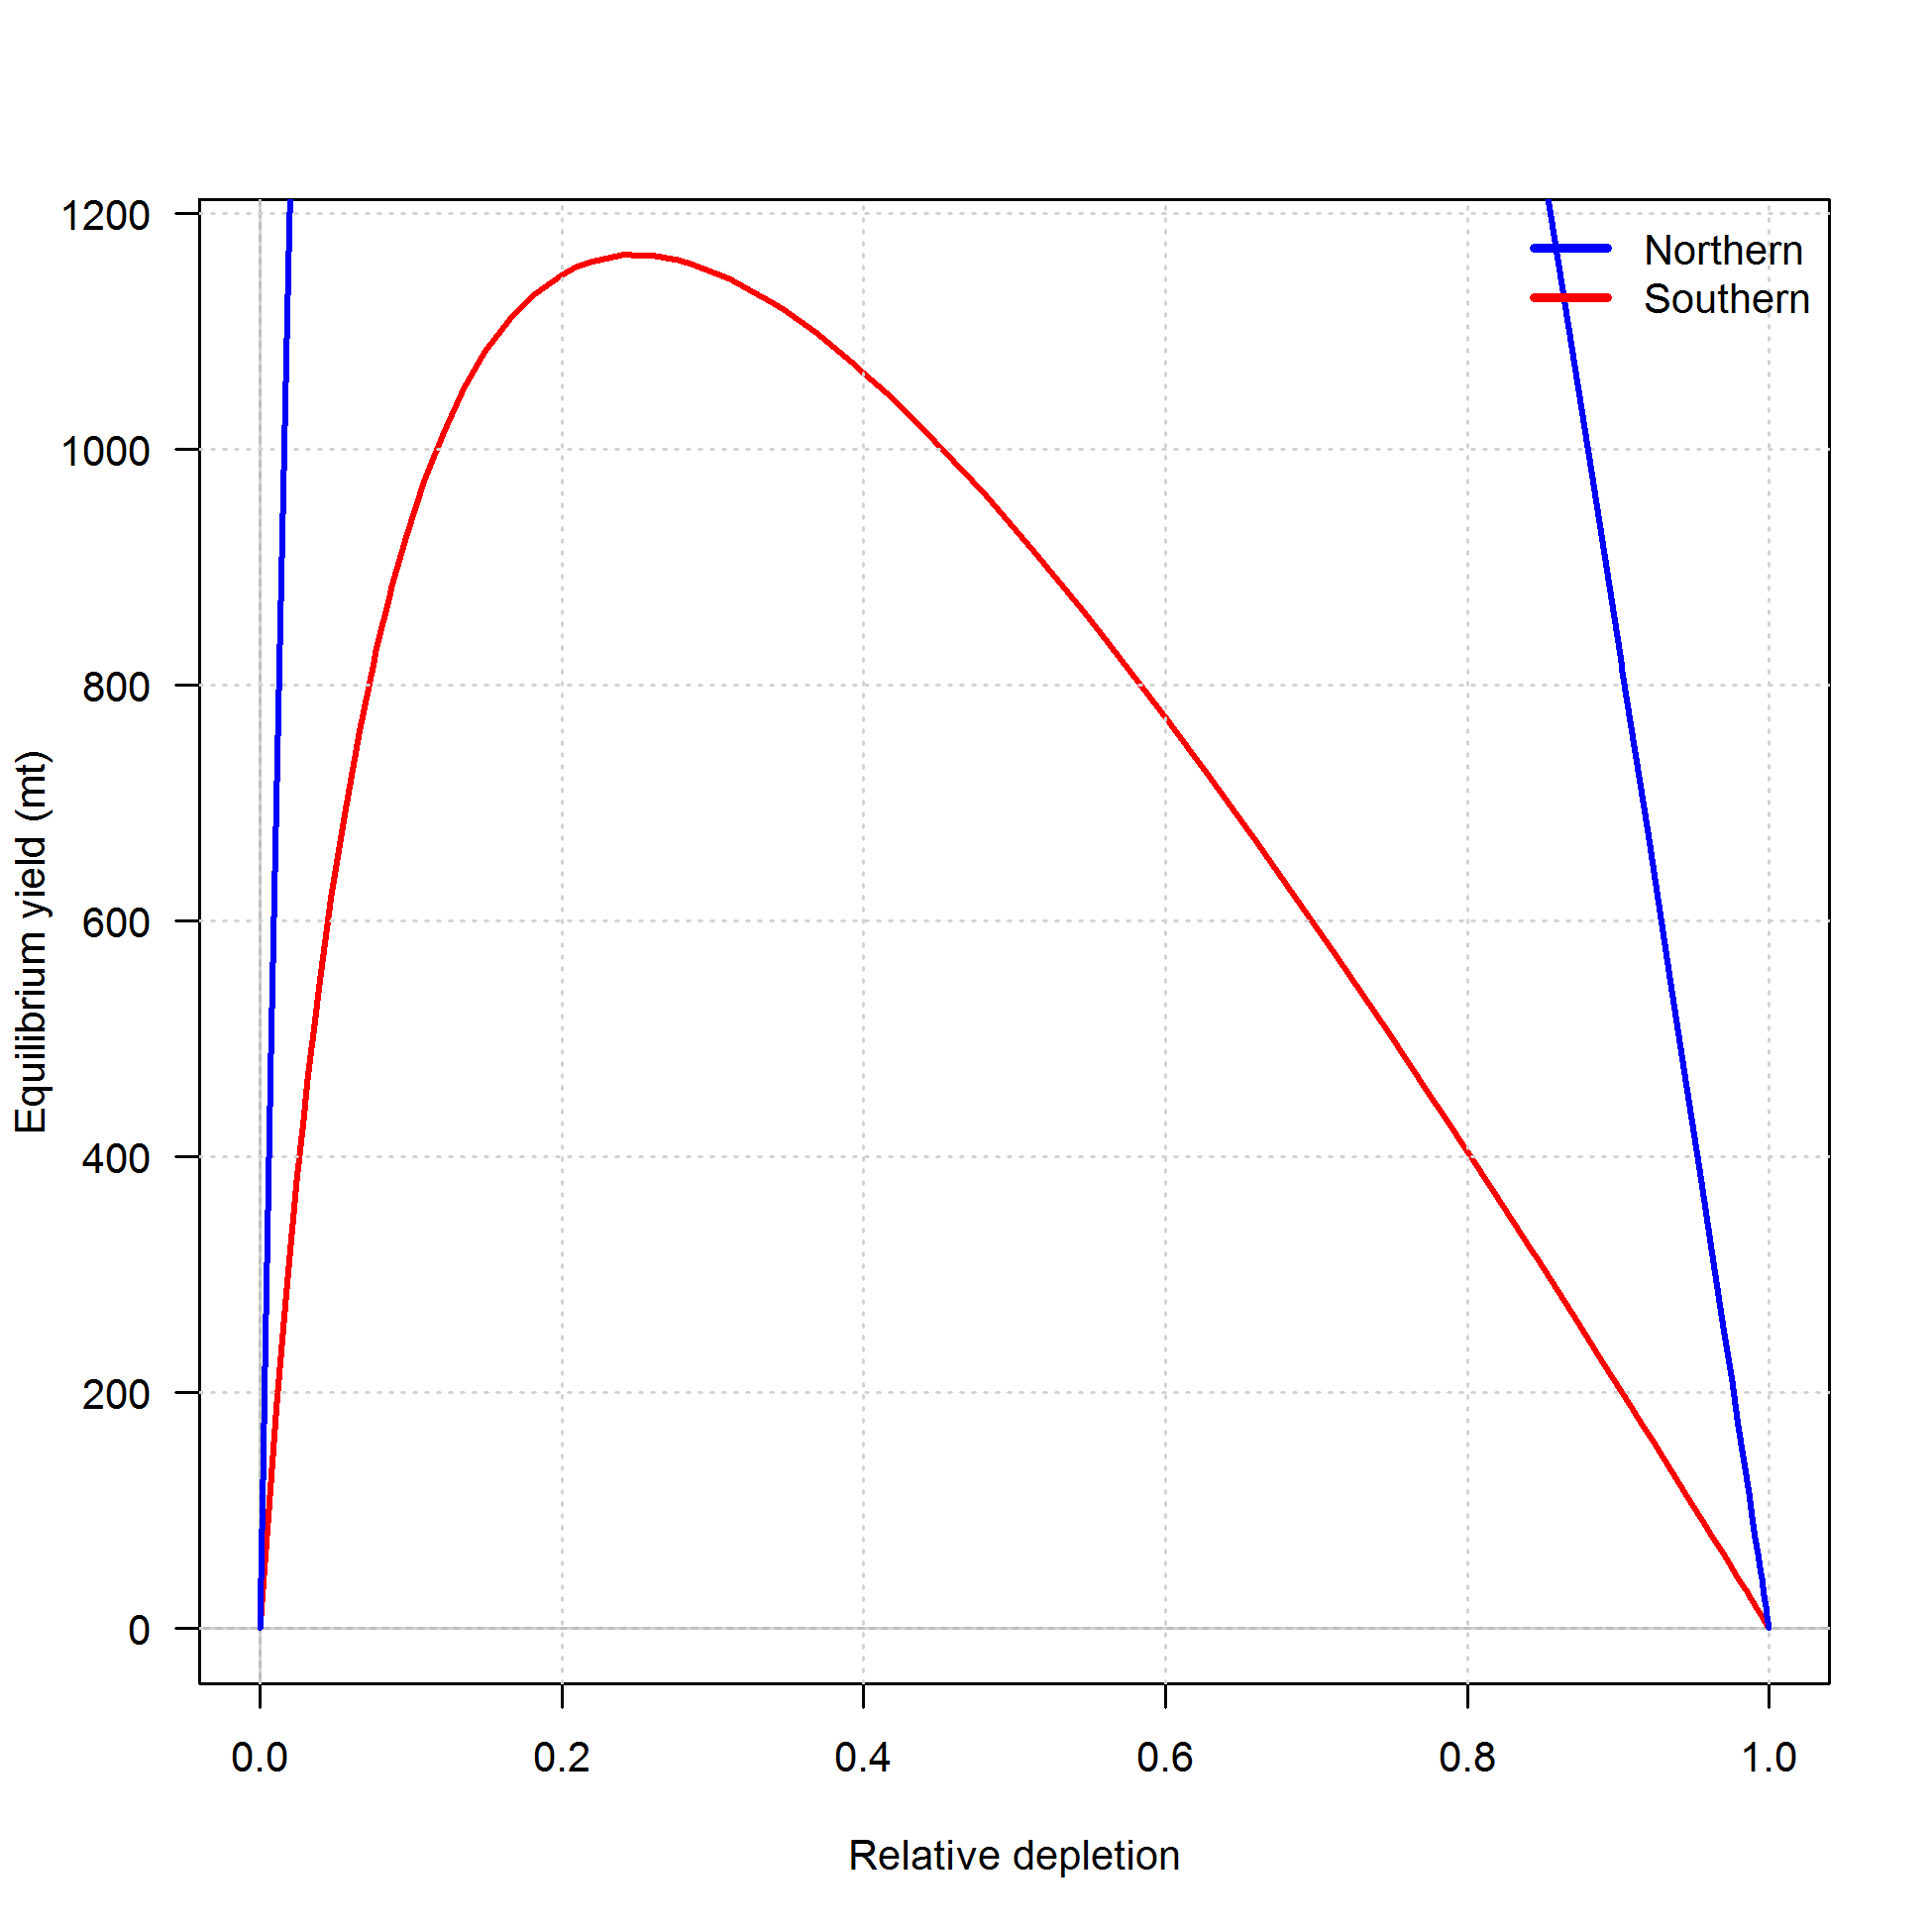
\includegraphics{r4ss/plots_compare/yield_comparison_n_models.png}
\caption{Equilibrium yield curve for the base case model. Values are
based on the 2016 fishery selectivity and with steepness fixed
at\ldots{} \label{fig:Yield_all}}
\end{figure}

\FloatBarrier

\newpage

\subsection*{Research And Data Needs}\label{research-and-data-needs}
\addcontentsline{toc}{subsection}{Research And Data Needs}

\hl{Include: identify information gaps that seriously impede the stock assessment.}

We recommend the following research be conducted before the next
assessment:

\begin{enumerate}

\item List item No. 1 in the list

\item List item No. 2 in the list, etc.

\end{enumerate}

\subsection*{Rebuilding Projections}\label{rebuilding-projections}
\addcontentsline{toc}{subsection}{Rebuilding Projections}

\hl{Include: reference to the principal results from rebuilding analysis if the 
stock is overfished. This section should be included in the Final/SAFE version 
assessment document but is not required for draft assessments undergoing review. 
See Rebuilding Analysis terms of reference for detailed information on 
rebuilding analysis requirements.}

\FloatBarrier

\newpage

\renewcommand{\thefigure}{\arabic{figure}}
\renewcommand{\thetable}{\arabic{table}}

\setcounter{figure}{0} \setcounter{table}{0} \pagenumbering{arabic}

\section{Introduction}\label{introduction}

\subsection{Basic Information}\label{basic-information}

\hl{Include: Scientific name, distribution, the basis of the choice of stock structure, 
including regional differences in life history or other biological characteristics 
that should form the basis of management units.}

\subsection{Map}\label{map}

A map showing the scope of the assessment and depicting boundaries for
fisheries or data collection strata is provided in Figure
\ref{fig:boundary_map}.

\subsection{Life History}\label{life-history}

\hl{Include: Important features of life history that affect management (e.g., migration, 
sexual dimorphism, bathymetric demography).}

\subsection{Ecosystem Considerations}\label{ecosystem-considerations-1}

\hl{Include: Ecosystem considerations (e.g., ecosystem role and trophic relationships of 
the species, habitat requirements/preferences, relevant data on ecosystem processes 
that may affect stock or parameters used in the stock assessment, and/or cross-FMP 
interactions with other fisheries). This section should note if environmental 
correlations or food web interactions were incorporated into the assessment model. 
The length and depth of this section would depend on availability of data and reports 
from the IEA, expertise of the STAT, and whether ecosystem factors are informational 
to contribute quantitative information to the assessment.}

\subsection{Fishery Information}\label{fishery-information}

\hl{Include: Important features of current fishery and relevant history of fishery.}

Rockfish example: The rockfish fishery off the U.S. Pacific coast first
developed off California in the late 19th century as a hook-and-line
fishery (Love et al. \protect\hyperlink{ref-Love2002}{2002}).\\
The rockfish trawl fishery was established in the early 1940s, when the
United States became involved in World War II and wartime shortage of
red meat created an increased demand for other sources of protein (Harry
and Morgan \protect\hyperlink{ref-Harry1961}{1961}, Alverson et al.
\protect\hyperlink{ref-Alverson1964}{1964}). Etc\ldots{}.

\subsection{Summary of Management
History}\label{summary-of-management-history}

\hl{Include: Summary of management history (e.g., changes in mesh sizes, trip 
limits, or other management actions that may have significantly altered selection, 
catch rates, or discards).}

\subsection{Management Performance}\label{management-performance-1}

\hl{Include: Management performance, including a table or tables comparing 
Overfishing Limit (OFL), Annual Catch Limit (ACL), Harvest Guideline (HG) 
[CPS only], landings, and catch (i.e., landings plus discard) for each area and year.}

Management performance table: (Table \ref{tab:mnmgt_perform})\\
A summary of these values as well as other base case summary results can
be found in Table \ref{tab:base_summary}.

\subsection{Fisheries off Canada, Alaska, and/or
Mexico}\label{fisheries-off-canada-alaska-andor-mexico}

Include if necessary.

\section{Data}\label{data}

Data used in the Northern and Southern yellowtail rockfish assessments
are summarized in Figures \ref{fig:data_plot} and \ref{fig:data_plot}.

Data sources for the two models are largely distinct. Northern fisheries
and surveys had very sparse data (if any) for the south and vice-versa.
Among the 12 data sources referenced below, only 2 data sources are
common to both models. These are the MRFSS/RecFIN recreational dockside
survey, which focuses on California and Oregon, and the CalCOM
California commercial dataset, which contributed data from the
northern-most California counties (Eureka and Del Norte) to the Northern
model. The CalCOM data account for less than five percent of the
commercial landings in the Northern model, and less than 1\% of the
biological samples.

Commercial landings are not differentiated in either model. For the
Northern model, this is due to the very small portion (1.15 \%) of the
landings that are attributed to non-trawl gear. For the Southern model,
this is due to the paucity of data.

A description of each model's data sources follows.

\subsection{Northern Model Data}\label{northern-model-data}

\begin{table}[ht]
\centering
\caption{Summary of the data source in the Northern model.} 
\label{tab:Data_sources}
\begin{tabular}{lllllll}
  \hline
Source & Landings & Lengths & Ages & Indices & Discard & Type \\ 
  \hline
PacFIN & Y & Y & Y & Y &  & Commercial \\ 
  WCGOP &  & Y &  &  & Y & Commercial Discards \\ 
  Hake Bycatch & Y & Y & Y & Y &  & Commercial \\ 
  CalCOM & Y & Y & Y &  &  & Commercial \\ 
  WaSport & Y & Y & Y &  &  & Recreational \\ 
  MRFSS & Y & Y &  &  &  & Recreational \\ 
  RecFIN & Y & Y &  &  &  & Recreational \\ 
  Triennial &  & Y & Y & Y &  & Survey \\ 
  NWFSCcombo &  & Y & Y & Y &  & Survey \\ 
  Pikitch &  & Y &  &  & Y & Commercial Study \\ 
  ODFW & Y &  &  &  &  & Historical data \\ 
  WDFW & Y &  &  &  &  & Historical data \\ 
   \hline
\end{tabular}
\end{table}

\subsubsection{Commercial Fishery
Landings}\label{commercial-fishery-landings}

\textbf{Washington and Oregon Landings} The bulk of the commercial
landings for Washington and Oregon came from the from the Pacific
Fisheries Information Network (\textbf{PacFIN}) database.

\textbf{Washington Catch Information}\\
The Washington Department of Fisheries and Wildlife (\textbf{WDFW})
provided historical yellowtail catch for 1889--1980. Landings for
1981-2016 came from the PacFIN database. WDFW also provided catches for
the period 1981 -- 2016 to include the re-distribution of the
unspeciated ``URCK'' landings in PacFIN; this information is currently
not available from PacFIN.

\textbf{Oregon Catch Information}\\
The Oregon Department of Fisheries and Wildlife (\textbf{ODFW}) provided
historical yellowtail catch from 1892-1985. ODFW also provided estimates
of yellowtail rockfish in the in the un-speciated PacFIN ``URCK'' and
``POP1'' catch categories for recent years, and those estimates were
combined with PacFIN landings for 1986-2016.

\textbf{Northern California Catch}\\
The California Commercial Fishery Database (\textbf{CalCOM}) provided
landings for the Northern model for the two counties north of 40.10
(Eureka and Del Norte) for 1969-2016.

\textbf{Hake Bycatch}\\
The Alaska Fisheries Science Center (\textbf{AFSC}) provided data for
yellowtail bycatch in the hake fishery from 1976-2016.

\subsubsection{Sport Fishery Removals}\label{sport-fishery-removals}

\textbf{Washington Sport Catch}\\
WDFW provided recreational catches for 1967 and 1975-2016.

\textbf{Oregon Sport Catch}\\
ODFW provided recreational catch data for 1979-2016.

\textbf{MRFSS and RecFIN} Data from Northern California came from the
Marine Recreational Fisheries Statistical Survey (\textbf{MRFSS}) and
from the Recreational Fisheries Information Network (**RecFIN). These
are dockside surveys focused on California and Oregon. MRFSS was
conducted from 1980-1989 and 1993-2003, RecFIN from 2004 to the present.

\subsubsection{Estimated Discards}\label{estimated-discards}

\textbf{Commercial Discards}\\
The West Coast Groundfish Observing Program (\textbf{WCGOP}) is an
onboard observer program that has extensively surveyed fishing practices
since 2002, with nearly 100\% observer coverage in the trawl sector in
recent years. WCGOP provided discard ratios for yellowtail rockfish from
2002 to 2015.

\textbf{Pikitch Study}\\
The Pikitch study was conducted between 1985 and 1987 (Pikitch et al.
\protect\hyperlink{ref-Pikitch1988}{1988}). The northern and southern
boundaries of the study were \(48^\circ 42^\prime\) N latitude and
\(42^\circ 60^\prime\) N. latitude respectively, which is primarily
within the Columbia INPFC area (Pikitch et al.
\protect\hyperlink{ref-Pikitch1988}{1988} , Rogers and Pikitch
\protect\hyperlink{ref-Rogers1992}{1992}).

Participation in the study was voluntary and included vessels using
bottom, midwater, and shrimp trawl gears.\\
Observers of normal fishing operations on commercial vessels collected
the data, estimated the total weight of the catch by tow and recorded
the weight of species retained and discarded in the sample.

Pikitch study discards were aggregated due to small sample size and
included in the data as representing a single year mid-way through the
study.

\subsubsection{Abundance Indices}\label{abundance-indices}

\textbf{Commercial Logbook CPUE}\\
The commercial logbook (fish-ticket) data in PacFIN was used to generate
an index for the years 1987-1998, a period in which management of the
fishery was stable, i.e., regulations weren``t changing fishery
practices.

The data were modeled with a modified Stephens-MacCall approach
(Stephens and MacCall \protect\hyperlink{ref-Stephens2004}{2004}). This
approach uses the species composition of the catch to evaluate the
per-haul probability of encountering a particular species; in this case,
yellowtail rockfish. The intent of the analysis is to eliminate all
hauls from the index that could not encounter yellowtail. Usually, the
Stephens-MacCall approach is a simple binomial model for
presence-absence of the predictive species and the target, however a
generalized linear mixed-effects approach -- modeling the species as
binomial and adding random effects for year, vessel, and haul-duration
improved the model fit.

The hauls identified with a reasonable probability of encountering
yellowtail were then modeled in a delta-lognormal glm to produce an
index of abundance.

\textbf{Hake Bycatch Index}\\
The Hake bycatch data provided by the Alaska Fisheries Science Center
(AFSC) was used to generate an index of abundance for 1985-1999.

Data on haul-by-haul catch of Yellowtail Rockfish and Pacific Hake for
the period 1976-2016 were obtained from the At-Sea Hake Observer Program
along associated information including the location of each tow and the
duration. Previous Yellowtail assessments used an index of abundance for
the years 1978-1999. The most recent assessment (Wallace and Lai, 2005)
stated that the index was not updated to include years beyond 1999
``because subsequent changes in fishery regulations and behavior have
altered the statistical properties of these abundance indices''. The
ending year of 1999 was retained for this analysis. However, the years
up to 1984 have relatively few tows with adequate information for CPUE
analysis, and fishing effort off the coast of Washington where
yellowtail are most commonly encountered (Figure X1). Therefore, for
this new analysis, 1985 was chosen as the starting year.

The hake fishery was evolving during the chosen 15 year period
(1985-1999), which included a transition from foreign to domestic fleets
fishing for Pacific Hake (Figure X2). The index from the at-sea hake
fishery used in previous assessments standardized for changes in
catchability by using a ratio estimator relating yellowtail catch to
hake catch and then scaling by an estimate of fishing effort for hake
(Equation 1 in Wallace and Lai, 2005). However, that approach does not
take into account differences in the spatial distribution of the at-sea
hake fishery relative to the distributions of hake and yellowtail.

For this new analysis, changes in catchability were estimated by
comparing an index based on a geostatistical analysis of the hake CPUE
from VAST (Thorson et al. YYYY) to the estimated available hake biomass
from the most recent stock assessment (Berger et al. 2017). The relative
catchability was then used to adjust an independent geostatistical index
of yellowtail CPUE (Figure X3). In order to capture the general trend in
catchability, reducing the variability among years, linear, exponential,
and locally smoothed (LOWESS) models were fit to the time series of
individual estimates of hake index to available biomass (Figure X3b). Of
these, the LOWESS model best captured the pattern of fastest change in
the middle of the time series. The average rate of increase in the
resulting estimated catchability time series is 13\% per year.

VAST was then used to conduct a geostatistical standardization of the
CPUE of yellowtail caught as bycatch in the at-sea hake fishery. The
resulting yellowtail index after adjustment by the estimated changes in
catchability is qualitatively more similar to the index used in previous
assessments (Figure X4) than the index resulting from assuming constant
catchability.

\textbf{Pikitch Study}\\
The Pikitch data referenced above provided an index for years 1981-91.

\subsubsection{Fishery-Independent Data}\label{fishery-independent-data}

\textbf{Northwest Fisheries Science Center (NWFSC) shelf-slope survey}\\
This survey, referred to as the \textbf{NWFSCcombo Survey}, has been
conducted annually since 2003.\\
The survey consistently covers depths between 30 and 700 fm.

Data from this survey for yellowtail rockfish was available for
2003-2016, and provided an index in addition to length and age data.

\textbf{Alaska Fisheries Science Center (AFSC) Triennial shelf survey}\\
The \textbf{Triennial Survey} was conducted by the AFSC every third year
between 1977 and 2001, (and was conducted in 2004 by the NWFSC using the
same protocols). The Triennial Survey trawled in depths of 30 to 275 fm.

The Triennial Survey provided yellowtail rockfish length and age data,
as well as an index of abundance from 1997-2004.

\subsubsection{Biological Samples}\label{biological-samples}

\textbf{Length And Age Compositions}\\
Length composition data were compiled from PacFIN for Oregon and
Washington for the Northern model and combined with raw (unexpanded)
length data from CalCOM for the two California counties north of 40.10
(Eureka and Del Norte counties).

Length compositions were provided from the following sources:

\begin{table}[ht]
\centering
\caption{Summary of the time series of lengths used in the stock assessment.} 
\label{tab:Length_sources}
\begin{tabular}{llrrl}
  \hline
Source & Type & Lengths & Tows & Years \\ 
  \hline
PacFIN & commercial & 186161 & 3830 & 1968-2016 \\ 
  CalCOM & commercial & 2340 &  & 1978-2015 \\ 
  MRFSS & recreational & 4125 &  & 1980-2003 \\ 
  RecFIN & recreational & 432 &  & 2004-2016 \\ 
  WASport & recreactional & 11099 &  & 1975-2015 \\ 
  Triennial & survey & 16262 & 465 & 1977-2004 \\ 
  NWFSCcombo & survey & 940 & 564 & 2004-2016 \\ 
   \hline
\end{tabular}
\end{table}

Model input sample-sizes for age data were calculated according to the
same algorithm as for lengths, except that the conditional age-at-length
sample sizes are the number of fish, regardless of the source of the
data.

Age structure data were available from the following sources:

\begin{table}[ht]
\centering
\caption{Summary of the
                                              time series of age data used in the stock
                                              assessment.} 
\label{tab:Age_sources}
\begin{tabular}{llrrl}
  \hline
Source & Type & Ages & Tows & Years \\ 
  \hline
PacFIN & commercial & 138854 &  & 1972-2016 \\ 
  CalCOM & commercial & 3546 &  & 1980-2002 \\ 
  WASport & recreational & 4027 &  & 1997-2016 \\ 
  Triennial & survey & 6553 & 278 & 1997-2004 \\ 
  NWFSCcombo & survey & 2990 & 544 & 2003-2016 \\ 
   \hline
\end{tabular}
\end{table}

\subsection{Southern Model Data}\label{southern-model-data}

\begin{table}[ht]
\centering
\caption{Summary of the data source in the Northern model.} 
\label{tab:Data_sources}
\begin{tabular}{lllllll}
  \hline
Source & Landings & Lengths & Ages & Indices & Discard & Type \\ 
  \hline
CalCOM & Y & Y & Y &  &  & Commercial \\ 
  MRFSS & Y & Y &  &  &  & Recreational \\ 
  RecFIN & Y & Y &  &  &  & Recreational \\ 
  HookandLine &  & Y & Y & Y &  & Survey \\ 
  Onboard &  & Y & Y & Y &  & Survey \\ 
  SmallResearch &  & Y & Y &  &  & Study \\ 
   \hline
\end{tabular}
\end{table}

\subsubsection{Commercial Fishery
Landings}\label{commercial-fishery-landings-1}

\textbf{California Commercial Landings}\\
The California Commercial Fishery Database (\textbf{CalCOM}) provided
landings in California south of 40.10 for 1969-2016.

\subsubsection{Sport Fishery Removals}\label{sport-fishery-removals-1}

\textbf{MRFSS Estimates and RecFIN}\\
The California Department of Fish and Wildlife (\textbf{CDFW}) provided
estimated yellowtail removals for the Marine Recreational Fisheries
Statistical Survey (\textbf{MRFSS}) from 1980-1989, 1993-2003. The
Recreational FIsheries Information Network, (\textbf{RecFIN}) provided
landings for 2004-2016.

\textbf{Small Research Study} A small number of fish were collected from
the recreational fishery by the Southwest Fisheries Science Center
(\textbf{SWFSC}) and are included in the data for 1978-1984.

\subsubsection{Estimated Discards}\label{estimated-discards-1}

No discard data were available for the Southern model.

\subsubsection{Abundance Indices}\label{abundance-indices-1}

\textbf{MRFSS Index}\\
An index of abundance was developed from trip-aggregated MRFSS data for
the years 1980-1989, 1992-2003.

\textbf{California Onboard Survey}\\
An Onboard recreational survey conducted by provided data for an index
of abundance provided by the SWFSC for 1987-2016.

\subsubsection{Fishery-Independent
Data}\label{fishery-independent-data-1}

\textbf{Hook and Line Survey}\\
The NWFSC Hook and Line survey provided data for an index in the
Southern California Bight from 2004-2016.

\subsubsection{Biological Samples}\label{biological-samples-1}

Length composition samples were available for the Southern model from 5
sources, and ages from 3.

Length compositions were provided from the following sources:

\begin{table}[ht]
\centering
\caption{Summary of the time series of lengths used in the stock assessment.} 
\label{tab:Length_sources}
\begin{tabular}{llrrl}
  \hline
Source & Type & Lengths & Tows & Years \\ 
  \hline
CalCOM & commercial & 16160 & 1543 & 1978-2015 \\ 
  MRFSS & recreational & 39425 &  & 1980-2003 \\ 
  RecFIN & recreational & 49136 &  & 2004-2016 \\ 
  Onboard & recreational & 76740 &  & 1987-2016 \\ 
  Small Study & recreational & 909 &  & 1978-1984 \\ 
  Hook and Line & survey & 1339 & 174 & 2004-2016 \\ 
   \hline
\end{tabular}
\end{table}

Model input sample-sizes for age data were calculated according to the
same algorithm as for lengths, except that the conditional age-at-length
sample sizes are the number of fish, regardless of the source of the
data.

Age structure data were available from the following sources:

\begin{table}[ht]
\centering
\caption{Summary of the
                                              time series of age data used in the stock
                                              assessment.} 
\label{tab:Age_sources}
\begin{tabular}{llrl}
  \hline
Source & Type & Ages & Years \\ 
  \hline
CalCOM & commercial & 7875 & 1980-2004 \\ 
  Small Study & recreational & 400 & 1978-1984 \\ 
  Hook and Line & survey & 248 & 2004 \\ 
   \hline
\end{tabular}
\end{table}

\subsection{Biological Parameters Common to Both
Models}\label{biological-parameters-common-to-both-models}

\vspace{.5cm}

\textbf{Aging Precision And Bias}

Age error matrices were developed for double-reads at the PFMC aging lab
in Newport, OR and for double reads within the WDFW aging lab. The
Newport lab has done all of the Survey aging for the NWFSC, along with
some commercial ages and the 400 fish from the Small Study. WDFW
provided the bulk of recreational and commercial ages. Between-lab
differences in aging were minute, as were within-lab differences.

\vspace{.5cm}

\textbf{Weight-Length}

The weight-length relationship is based on the standard power function:
\(W = \alpha(L^\beta)\) where \(W\) is individual weight (kg), \(L\) is
length (cm), and \(\alpha\) and \(\beta\) are coefficients used as
constants.

To estimate this relationship, 12,778 samples with both weight and
length measurements from the fishery independent surveys were analyzed.
These included 6,354 samples from the NWFSC Combo survey, 5,085 from the
Triennial survey, and 1,339 from the Hook and Line survey. All Hook and
Line survey samples were from the Southern area, along with 910 samples
from the other two surveys (Figure \ref{fig:weight-length}). A single
weight-length relationship was chosen for females and males in both
areas after examining various factors that may influence this
relationships, including sex, area, year, and season. None of these
factors had a strong influence in the overall results. Season was one of
the bigger factors, with fish sampled later in the year showing a small
increase in weight at a given length (2-6\% depending on the other
factors considered). However, season was confounded with area because
most of the samples from the Southern area were collected from the Hook
and Line survey which takes place later in the year (mid-September to
mid-November) and the resolution of other data in the model do not
support modeling the stock at a scale finer than a annual time step.
Males and females did not show strong differences in either area, and
the estimated differences were in opposite directions for the two areas,
suggesting that this might be a spurious relationship or confounded with
differences timing of the sampling relative to spawning.

The estimated coefficients resulting from this analysis were
\(\alpha = 1.1843e-05\) and \(\beta = 3.0672\).

\vspace{.5cm}

\textbf{Maturity And Fecundity} Maturity was estimated from histological
analysis of

141 samples collected in 2016. These include 96 from the NWFSC Combo
survey, 25 from mid-water catches in the NWFSC acoustic/trawl survey, 13
from the Hook and Line survey, and 7 from Oregon Department of Fish and
Wildlife. The sample sizes were not adequate to estimate differences in
maturity by area. Length at 50\% maturity was estimated at 42.49cm
(Figure \ref{fig:maturity.png}) which was consistent with the range
37-45cm cited in the previous assessment (Wallace and Lai
\protect\hyperlink{ref-Wallace2005}{2005}).

\vspace{.5cm}

\textbf{Natural Mortality}

Natural mortality estimates used as priors for the Northern model and as
fixed values for the Southern model were provided by Owen Hamel (pers.
comm.).

\vspace{.5cm}

\textbf{Sex ratios}

The largest fish seen in the data are females, however the oldest are
males. The sex ratio falls off differently in each model, as can be seen
in Figs(x,y).

\subsubsection{Environmental Or Ecosystem Data Included In The
Assessment}\label{environmental-or-ecosystem-data-included-in-the-assessment}

No environmental index is present in either model.

\section{Assessment}\label{assessment}

\subsection{History Of Modeling Approaches Used For This
Stock}\label{history-of-modeling-approaches-used-for-this-stock}

Yellowtail rockfish was previously modeled as a 3-area stock north of
40.10 using ADMB in 1999 Need citation, with an update assessment in
2004(Wallace and Lai \protect\hyperlink{ref-Wallace2005}{2005}). That
assessment divided the stock into 3 INPFC areas which are not coincident
with state boundaries; this is a concern in that recent reconstructions
of historical catch are state-by-state along the West Coast, therefor we
have made no effort to reproduce the previous model.

\subsubsection{Previous Assessment
Recommendations}\label{previous-assessment-recommendations}

Include: Response to STAR panel recommendations from the most recent
previous assessment.

\begin{description}[style=unboxed]

  \item[Recommendation 1: More data needed.] \hfill \\

   STAT response: Got some.

\item[Recommendation 2: blah blah blah.] \hfill \\

  STAT response: blah blah blah....

\item[Recommendation 3: blah blah blah., etc.] \hfill \\

  STAT response: Continue recommendations as needed


\end{description}

\subsection{Model Description}\label{model-description}

\subsubsection{Transition To The Current Stock
Assessment}\label{transition-to-the-current-stock-assessment}

These are the main changes from the previous model, and our rationale
for them:

\begin{enumerate}
\def\labelenumi{\arabic{enumi}.}
\item
  Transition to Stock Synthesis. \emph{Rationale}: The Pacific Fishery
  Management Council's preferred modeling platform for stock assessments
  is Stock Synthesis (Methot \protect\hyperlink{ref-Methot2015}{2015}),
  developed since the last full assessment of yellowtail rockfish.
\item
  Addition of Southern model. \emph{Rationale}: Hess, et al. determined
  that the West Coast yellowtail stocks show a genetic cline occurring
  near Cape Mendocino, which is roughly 40.10 north latitude (Hess et
  al. n.d.). This divides the stock into two genetically distinct
  substocks which we model independently.
\item
  Availability of recent data. \emph{Rationale}: Ten years of data
  collection have occurred since the last update assessment.
\item
  Historical catch reconstructions. \emph{Rationale}: Reconstruction of
  catch timeseries in California, Washington and Oregon clarify stock
  history as far back as 1898.
\end{enumerate}

\subsubsection{Definition of Fleets and
Areas}\label{definition-of-fleets-and-areas}

\textbf{Northern Model}

\emph{Commercial}: The commercial fleet consists primarily of bottom and
midwater trawl.

\emph{Recreational}: The recreational fleet includes data from sport
fisheries off Washington, Oregon, and northern California (Eureka and
Del Norte counties)

\emph{Research}: Research derived-data include observations from the
West Coast Groundfish Observing Program (WCGOP) which documents
discarding in the commercial fishery, the Alaska Fisheries Science
Center's Triennial Trawl survey, and the Northwest Fisheries Science
Center's NWFSCcombo survey.

\textbf{Southern Model}

\emph{Commercial}: The commercial fleet consists primarily of hook and
line and trawl gear. Hook and line gear account for 78\% of the landings
by weight in the recent period (1978-2016).

\emph{Recreational}: The recreational fleet includes data from sport
fishery off the California coast south of Cape Mendocino.

\emph{Research}: Research derived-data include observations from the
Northwest Fisheries Science Center's NWFSCcombo survey, and California
Onboard recreational survey.

\subsubsection{Modeling Software}\label{modeling-software}

The STAT team used Stock Synthesis 3 version 3.3 (Methot
\protect\hyperlink{ref-Methot2015}{2015}).

\subsubsection{Data Weighting}\label{data-weighting}

Commercial and survey length composition and marginal age composition
data are weighted according to the method of Ian Stewart (pers.comm):

Sample Size = 0.138 * Nfish + Ntows if Nfish/Ntows \textless{} 44, and
Ntows * 7.06 otherwise.

Age-at-Length samples are unwieghted; that is, each fish is assumed to
represesnt an independent sample.

Recreational tows are difficult to define in most cases. Since much of
the recreational data are from the dockside interview Marine
Recreational Fisheries Statics Survey (MRFSS, 1980-2003), which provided
notoriously poor data with respect to aggregating samples to ``trip'',
we chose to use all recreational data ``as-is'', with the initial
weights entered as number of fish.

Stock Synthesis does internal re-weighting between years within fleets
to adjust for sample size. Weighting among fleets uses either the
Francis method (Francis \protect\hyperlink{ref-Francis2011}{2011}) or
the Ianelli-McAllister harmonic mean method (McAllister and Ianelli
\protect\hyperlink{ref-McAllister1997}{1997}). The Francis method was
used for all fleets, except for the Southern model's Hook and Line age
data, which is a single year of data to which we applied the
Ianelli-McAllister method.

\subsubsection{Priors}\label{priors}

Natural Mortality (M) priors were provide by Owen Hamel prior on natural
mortality (Hamel \protect\hyperlink{ref-Hamel2015}{2015}). We used the
Hamel prior as a fixed value in the Southern model, however the Northern
model was able to estimate M. In both models, male M was estimated as an
offset from female M. The Southern female M is 0.18; the Northern female
M prior is 0.12.

The prior for steepness (h, 0.718) was provided by James Thorson and
used as a fixed parameter in both models. \textless{}TOADS:
Citation\textgreater{}

\subsubsection{General Model
Specifications}\label{general-model-specifications}

Citation for posterior predictive fecundity relationship from Dick
(\protect\hyperlink{ref-Dick2009}{2009})\\
Model data, control, starter, and forecast files can be found at
\url{https://DEVORE} .

\subsubsection{Estimated And Fixed
Parameters}\label{estimated-and-fixed-parameters}

A full list of all estimated and fixed parameters is provided in
Tables\ldots{}. Estimated and fixed parameters tables currently read in
from .csv file, EXAMPLE: Table \ref{tab:Model1_params}

\subsection{Model Selection and
Evaluation}\label{model-selection-and-evaluation}

\subsubsection{Key Assumptions and Structural
Choices}\label{key-assumptions-and-structural-choices}

Include: Evidence of search for balance between model realism and
parsimony.\\
Comparison of key model assumptions, include comparisons based on nested
models (e.g., asymptotic vs.~domed selectivities, constant
vs.~time-varying selectivities).

Selectivity in both models is asymptotic, with the exception of the
OR-CA MRFSS recreational fleet in the Northern model, and the Onboard
recreational fleet in the Southern model.

\subsubsection{Alternate Models
Considered}\label{alternate-models-considered}

Include: Summary of alternate model configurations that were tried but
rejected.

\subsubsection{Convergence}\label{convergence}

Include: Randomization run results or other evidence of search for
global best estimates.

Convergence testing through use of dispersed starting values often
requires extreme values to actually explore new areas of the
multivariate likelihood surface. Jitter is a Stock Synthesis option that
generates random starting values from a normal distribution logistically
transformed into each parameter's range (Methot
\protect\hyperlink{ref-Methot2015}{2015}). Table \ref{tab:jitter} shows
the results of running 100 jitters for each pre-STAR base model\ldots{}.

\subsection{Response To The Current STAR Panel
Requests}\label{response-to-the-current-star-panel-requests}

\begin{description}[style=unboxed]

\item[Request No. 1: Add after STAR panel.] \hfill \\

    \textbf{Rationale:} Add after STAR panel.  

    \textbf{STAT Response:} Add after STAR panel.

\item[Request No. 2: Add after STAR panel.] \hfill \\

    \textbf{Rationale:} Add after STAR panel.

    \textbf{STAT Response:} Add after STAR panel.

\item[Request No. 3: Add after STAR panel.] \hfill \\

    \textbf{Rationale:} Add after STAR panel.
  
    \textbf{STAT Response:} Add after STAR panel.

\item[Request No. 4: Example of a request that may have a list:] \hfill \\
\begin{itemize}
\item \textbf{Item No. 1}
\item \textbf{Item No. 2}
\item \textbf{Item No. 3, etc.}
\end{itemize}

    \textbf{Rationale:} Add after STAR panel.

    \textbf{STAT Response:} Continue requests as needed.


\end{description}

\subsection{Model 1}\label{model-1}

\subsubsection{Model 1 Base Case
Results}\label{model-1-base-case-results}

Table \ref{tab:Model1_params}

\subsubsection{Model 1 Uncertainty and Sensitivity
Analyses}\label{model-1-uncertainty-and-sensitivity-analyses}

Table \ref{tab:Sensitivity_model1}

\subsubsection{Model 1 Retrospective
Analysis}\label{model-1-retrospective-analysis}

\subsubsection{Model 1 Likelihood
Profiles}\label{model-1-likelihood-profiles}

\subsubsection{Model 1 Harvest Control Rules (CPS
only)}\label{model-1-harvest-control-rules-cps-only}

\subsubsection{Model 1 Reference Points (groundfish
only)}\label{model-1-reference-points-groundfish-only}

Intro sentence or two\ldots{}.(Table \ref{tab:Timeseries_mod1}).

Equilibrium yield at the proxy \(F_{MSY}\) harvest rate corresponding to
\(SPR_{50\%}\) is 3691.6 mt. Table \ref{tab:Ref_pts_mod1} shows the full
suite of estimated reference points for the northern area model and
Figure \ref{fig:Yield_all} shows the equilibrium yield curve.

\subsection{Model 2}\label{model-2}

\subsubsection{Model 2 Base Case
Results}\label{model-2-base-case-results}

\subsubsection{Model 2 Uncertainty and Sensitivity
Analyses}\label{model-2-uncertainty-and-sensitivity-analyses}

\subsubsection{Model 2 Retrospective
Analysis}\label{model-2-retrospective-analysis}

\subsubsection{Model 2 Likelihood
Profiles}\label{model-2-likelihood-profiles}

\subsubsection{Model 2 Harvest Control Rules (CPS
only)}\label{model-2-harvest-control-rules-cps-only}

\subsubsection{Model 2 Reference Points (groundfish
only)}\label{model-2-reference-points-groundfish-only}

\subsection{Model 3}\label{model-3}

\subsubsection{Model 3 Base Case
Results}\label{model-3-base-case-results}

\subsubsection{Model 3 Uncertainty and Sensitivity
Analyses}\label{model-3-uncertainty-and-sensitivity-analyses}

\subsubsection{Model 3 Retrospective
Analysis}\label{model-3-retrospective-analysis}

\subsubsection{Model 3 Likelihood
profiles}\label{model-3-likelihood-profiles}

\subsubsection{Model 3 Harvest Control Rules (CPS
only)}\label{model-3-harvest-control-rules-cps-only}

\subsubsection{Model 3 Reference Points (groundfish
only)}\label{model-3-reference-points-groundfish-only}

\section{Harvest Projections and Decision
Tables}\label{harvest-projections-and-decision-tables}

Table \ref{tab:mnmgt_perform}

\textbf{Model 1 Projections and Decision Table (groundfish only)} (Table
\ref{tab:Forecast_mod1}

Table \ref{tab:Decision_table_mod1}

\textbf{Model 2 Projections and Decision Table (groundfish only)}

\textbf{Model 3 Projections and Decision Table (groundfish only)}

\section{Regional Management
Considerations}\label{regional-management-considerations}

\begin{enumerate}
\def\labelenumi{\arabic{enumi}.}
\tightlist
\item
  For stocks where current practice is to allocate harvests by
  management area, a recommended method of allocating harvests based on
  the distribution of biomass should be provided. The MT advisor should
  be consulted on the appropriate management areas for each stock.
\item
  Discuss whether a regional management approach makes sense for the
  species from a biological perspective.
\item
  If there are insufficient data to analyze a regional management
  approach, what are the research and data needs to answer this
  question?
\end{enumerate}

\section{Research Needs}\label{research-needs}

\begin{enumerate}

\item Research need No. 1

\item Research need No. 2

\item Research need No. 3

\item etc.

\end{enumerate}

\section{Acknowledgments}\label{acknowledgments}

Include: STAR panel members and affiliations as well as names and
affiliations of persons who contributed data, advice or information but
were not part of the assessment team. Not required in draft assessment
undergoing review.

\newpage

\FloatBarrier

\section{Tables}\label{tables}

\FloatBarrier

\FloatBarrier

\begin{landscape}
\begin{longtable}{rlrrcccl}
\caption{List of parameters used in
                                              the base model, including estimated 
                                              values and standard deviations (SD), 
                                              bounds (minimum and maximum), 
                                              estimation phase (negative values indicate
                                              not estimated), status (indicates if 
                                              parameters are near bounds, and prior type
                                              information (mean, SD).} \\ 
  \hline
No. & Parameter & Value & Phase & Bounds & Status & SD & Prior (Exp.Val, SD)  \\ 
  \hline 
\endhead 
\hline 
\multicolumn{3}{l}{\footnotesize Continued on next page} 
\endfoot 
\endlastfoot 
 \hline
1 & NatM\_p\_1\_Fem\_GP\_1 & 0.141 & 2 & (0.02, 0.25) & OK & 0.009 & None \\ 
  2 & L\_at\_Amin\_Fem\_GP\_1 & 14.879 & 3 & (1, 25) & OK & 0.575 & None \\ 
  3 & L\_at\_Amax\_Fem\_GP\_1 & 53.827 & 2 & (35, 70) & OK & 0.235 & None \\ 
  4 & VonBert\_K\_Fem\_GP\_1 & 0.137 & 3 & (0.1, 0.4) & OK & 0.004 & None \\ 
  5 & CV\_young\_Fem\_GP\_1 & 0.101 & 5 & (0.03, 0.16) & OK & 0.010 & None \\ 
  6 & CV\_old\_Fem\_GP\_1 & 0.043 & 5 & (0.03, 0.16) & OK & 0.003 & None \\ 
  7 & Wtlen\_1\_Fem & 0.000 & -50 & (0, 3) &  &  & None \\ 
  8 & Wtlen\_2\_Fem & 3.067 & -50 & (2, 4) &  &  & None \\ 
  9 & Mat50\%\_Fem & 42.490 & -50 & (30, 56) &  &  & None \\ 
  10 & Mat\_slope\_Fem & -0.401 & -50 & (-2, 1) &  &  & None \\ 
  11 & Eggs\_scalar\_Fem & 0.000 & -50 & (0, 6) &  &  & None \\ 
  12 & Eggs\_exp\_len\_Fem & 4.590 & -50 & (2, 7) &  &  & None \\ 
  13 & NatM\_p\_1\_Mal\_GP\_1 & -0.142 & 2 & (-3, 3) & OK & 0.017 & None \\ 
  14 & L\_at\_Amin\_Mal\_GP\_1 & 0.000 & -2 & (-1, 1) &  &  & None \\ 
  15 & L\_at\_Amax\_Mal\_GP\_1 & -0.148 & 2 & (-1, 1) & OK & 0.005 & None \\ 
  16 & VonBert\_K\_Mal\_GP\_1 & 0.369 & 3 & (-1, 1) & OK & 0.027 & None \\ 
  17 & CV\_young\_Mal\_GP\_1 & 0.000 & -5 & (-1, 1) &  &  & None \\ 
  18 & CV\_old\_Mal\_GP\_1 & 0.172 & 5 & (-1, 1) & OK & 0.070 & None \\ 
  19 & Wtlen\_1\_Mal & 0.000 & -50 & (0, 3) &  &  & None \\ 
  20 & Wtlen\_2\_Mal & 3.067 & -50 & (2, 4) &  &  & None \\ 
  24 & CohortGrowDev & 1.000 & -50 & (0, 2) &  &  & None \\ 
  25 & FracFemale\_GP\_1 & 0.500 & -99 & (0.001, 0.999) &  &  & None \\ 
  26 & SR\_LN(R0) & 10.181 & 1 & (5, 20) & OK & 0.158 & None \\ 
  27 & SR\_BH\_steep & 0.718 & -6 & (0.2, 1) &  &  & None \\ 
  28 & SR\_sigmaR & 0.546 & -6 & (0.5, 1.2) &  &  & None \\ 
  29 & SR\_regime & 0.000 & -50 & (-5, 5) &  &  & None \\ 
  30 & SR\_autocorr & 0.000 & -50 & (0, 2) &  &  & None \\ 
  140 & LnQ\_base\_CommercialTrawl(1) & -4.397 & -1 & (-30, 15) &  &  & None \\ 
  141 & LnQ\_base\_HakeByCatch(2) & -9.820 & -1 & (-30, 15) &  &  & None \\ 
  142 & Q\_extraSD\_HakeByCatch(2) & 0.278 & 1 & (0, 0.5) & OK & 0.083 & None \\ 
  143 & LnQ\_base\_Triennial(5) & -1.003 & -1 & (-30, 15) &  &  & None \\ 
  144 & LnQ\_base\_NWFSCcombo(6) & -0.559 & -1 & (-30, 15) &  &  & None \\ 
  145 & SizeSel\_P1\_CommercialTrawl(1) & 48.717 & 1 & (20, 55) & OK & 0.724 & None \\ 
  146 & SizeSel\_P2\_CommercialTrawl(1) & 70.000 & -4 & (-20, 70) &  &  & None \\ 
  147 & SizeSel\_P3\_CommercialTrawl(1) & 4.296 & 3 & (-5, 20) & OK & 0.095 & None \\ 
  148 & SizeSel\_P4\_CommercialTrawl(1) & 70.000 & -4 & (-5, 70) &  &  & None \\ 
  149 & SizeSel\_P5\_CommercialTrawl(1) & -999.000 & -99 & (-999, 25) &  &  & None \\ 
  150 & SizeSel\_P6\_CommercialTrawl(1) & -999.000 & -99 & (-999, 25) &  &  & None \\ 
  151 & Retain\_P1\_CommercialTrawl(1) & 24.506 & 3 & (20, 55) & OK & 3.272 & None \\ 
  152 & Retain\_P2\_CommercialTrawl(1) & 1.597 & 3 & (0.1, 40) & OK & 0.700 & None \\ 
  153 & Retain\_P3\_CommercialTrawl(1) & 3.070 & 3 & (-10, 20) & OK & 0.706 & None \\ 
  154 & Retain\_P4\_CommercialTrawl(1) & 0.000 & -4 & (-3, 3) &  &  & None \\ 
  155 & SizeSel\_P1\_HakeByCatch(2) & 52.341 & 1 & (20, 55) & OK & 0.878 & None \\ 
  156 & SizeSel\_P2\_HakeByCatch(2) & 70.000 & -4 & (-20, 70) &  &  & None \\ 
  157 & SizeSel\_P3\_HakeByCatch(2) & 4.301 & 3 & (-5, 20) & OK & 0.113 & None \\ 
  158 & SizeSel\_P4\_HakeByCatch(2) & 70.000 & -4 & (-5, 70) &  &  & None \\ 
  159 & SizeSel\_P5\_HakeByCatch(2) & -999.000 & -99 & (-999, 25) &  &  & None \\ 
  160 & SizeSel\_P6\_HakeByCatch(2) & -999.000 & -99 & (-999, 25) &  &  & None \\ 
  161 & SizeSel\_P1\_RecORandCA(3) & 30.578 & 1 & (20, 55) & OK & 0.710 & None \\ 
  162 & SizeSel\_P2\_RecORandCA(3) & -19.161 & 4 & (-20, 7) & OK & 3239.790 & None \\ 
  163 & SizeSel\_P3\_RecORandCA(3) & 3.117 & 3 & (-5, 20) & OK & 0.237 & None \\ 
  164 & SizeSel\_P4\_RecORandCA(3) & 6.734 & 4 & (-5, 20) & OK & 0.566 & None \\ 
  165 & SizeSel\_P5\_RecORandCA(3) & -999.000 & -99 & (-999, 25) &  &  & None \\ 
  166 & SizeSel\_P6\_RecORandCA(3) & -999.000 & -99 & (-999, 25) &  &  & None \\ 
  167 & SizeSel\_P1\_RecWA(4) & 28.338 & 6 & (20, 55) & OK & 0.950 & None \\ 
  168 & SizeSel\_P2\_RecWA(4) & 70.000 & -4 & (-20, 70) &  &  & None \\ 
  169 & SizeSel\_P3\_RecWA(4) & -1.407 & 6 & (-5, 20) & OK & 2.463 & None \\ 
  170 & SizeSel\_P4\_RecWA(4) & 70.000 & -4 & (-5, 70) &  &  & None \\ 
  171 & SizeSel\_P5\_RecWA(4) & -999.000 & -99 & (-999, 25) &  &  & None \\ 
  172 & SizeSel\_P6\_RecWA(4) & -999.000 & -99 & (-999, 25) &  &  & None \\ 
  173 & SizeSel\_P1\_Triennial(5) & 54.364 & 1 & (20, 55) & OK & 3.966 & None \\ 
  174 & SizeSel\_P2\_Triennial(5) & 70.000 & -4 & (-20, 70) &  &  & None \\ 
  175 & SizeSel\_P3\_Triennial(5) & 5.128 & 3 & (-5, 20) & OK & 0.308 & None \\ 
  176 & SizeSel\_P4\_Triennial(5) & 70.000 & -4 & (-5, 70) &  &  & None \\ 
  177 & SizeSel\_P5\_Triennial(5) & -999.000 & -99 & (-999, 25) &  &  & None \\ 
  178 & SizeSel\_P6\_Triennial(5) & -999.000 & -99 & (-999, 25) &  &  & None \\ 
  179 & SizeSel\_P1\_NWFSCcombo(6) & 49.696 & 1 & (20, 55) & OK & 2.906 & None \\ 
  180 & SizeSel\_P2\_NWFSCcombo(6) & 70.000 & -4 & (-20, 70) &  &  & None \\ 
  181 & SizeSel\_P3\_NWFSCcombo(6) & 4.551 & 3 & (-5, 20) & OK & 0.433 & None \\ 
  182 & SizeSel\_P4\_NWFSCcombo(6) & 70.000 & -4 & (-5, 70) &  &  & None \\ 
  183 & SizeSel\_P5\_NWFSCcombo(6) & -999.000 & -99 & (-999, 25) &  &  & None \\ 
  184 & SizeSel\_P6\_NWFSCcombo(6) & -999.000 & -99 & (-999, 25) &  &  & None \\ 
  185 & Retain\_P3\_CommercialTrawl(1)\_BLK1repl\_2002 & 2.228 & 6 & (-10, 20) & OK & 0.457 & None \\ 
  186 & Retain\_P3\_CommercialTrawl(1)\_BLK1repl\_2003 & 3.708 & 6 & (-10, 20) & OK & 0.756 & None \\ 
  187 & Retain\_P3\_CommercialTrawl(1)\_BLK1repl\_2004 & 1.128 & 6 & (-10, 20) & OK & 0.522 & None \\ 
  188 & Retain\_P3\_CommercialTrawl(1)\_BLK1repl\_2005 & -0.115 & 6 & (-10, 20) & OK & 0.400 & None \\ 
  189 & Retain\_P3\_CommercialTrawl(1)\_BLK1repl\_2006 & 1.760 & 6 & (-10, 20) & OK & 0.260 & None \\ 
  190 & Retain\_P3\_CommercialTrawl(1)\_BLK1repl\_2007 & -0.516 & 6 & (-10, 20) & OK & 0.625 & None \\ 
  191 & Retain\_P3\_CommercialTrawl(1)\_BLK1repl\_2008 & 2.373 & 6 & (-10, 20) & OK & 0.820 & None \\ 
  192 & Retain\_P3\_CommercialTrawl(1)\_BLK1repl\_2009 & 0.480 & 6 & (-10, 20) & OK & 0.495 & None \\ 
  193 & Retain\_P3\_CommercialTrawl(1)\_BLK1repl\_2010 & 0.159 & 6 & (-10, 20) & OK & 0.678 & None \\ 
  194 & Retain\_P3\_CommercialTrawl(1)\_BLK1repl\_2011 & 7.327 & 6 & (-10, 20) & OK & 0.670 & None \\ 
   \hline
\hline
\label{tab:model_params}
\end{longtable}
\end{landscape}

\newpage

\begin{table}[ht]
\centering
\caption{Summary of the biomass/abundance
                                              time series used in the stock
                                              assessment.} 
\label{tab:Index_summary}
\begin{tabular}{>{\centering}p{.4in}>{\centering}p{.3in}>{\centering}p{.3in}>{\centering}p{.3in}>{\centering}p{.6in}>{\centering}p{.5in}>{\centering}p{.8in}>{\centering}p{.8in}>{\centering}p{.5in}}
  \hline
Region & ID & Fleet & Years & Name & Fishery ind. & Filtering & Method & Endorsed \\ 
  \hline
WA & 1 & 4 & 1981-2014 & Dockside CPUE & No & trip, area, month, Stephens-MacCall & delta-GLM (bin-gamma) & SSC \\ 
  - & - & - & - & - & - & - & - & - \\ 
  - & - & - & - & - & - & - & - & - \\ 
  - & - & - & - & - & - & - & - & - \\ 
   \hline
\end{tabular}
\end{table}

\newpage

\begin{table}[ht]
\centering
\caption{Results from 100 jitters from each of 
                                      the three models.} 
\label{tab:jitter}
\begin{tabular}{llll}
  \hline
Status & Model.1 & Model.2 & Model.3 \\ 
  \hline
Returned to base case & - & - & - \\ 
  Found local minimum & - & - & - \\ 
  Found better solution & - & - & - \\ 
  Error in likelihood & - & - & - \\ 
  Total & 100 & 100 & 100 \\ 
   \hline
\end{tabular}
\end{table}

\FloatBarrier

\newpage

\begin{sidewaystable}[ht]
\centering
\caption{Sensitivity of the base model 
                                          to dropping or down-weighting data 
                                          sources and alternative assumptions 
                                          about growth.} 
\label{tab:Sensitivity_model1}
\scalebox{0.9}{
\begin{tabular}{l>{\centering}p{.6in}>{\centering}p{.6in}>{\centering}p{.6in}>{\centering}p{.6in}>{\centering}p{.6in}>{\centering}p{.6in}>{\centering}p{.6in}>{\centering}p{.6in}}
  \hline
Label & Base (Francis weights) & Harmonic mean weights & Drop index & Drop ages & Down-weight lengths & Free size Age0 & Free CV Amin & External growth \\ 
  \hline
TOTAL\_like & - & - & - & - & - & - & - & - \\ 
  Catch\_like & - & - & - & - & - & - & - & - \\ 
  Equil\_catch\_like & - & - & - & - & - & - & - & - \\ 
  Survey\_like & - & - & - & - & - & - & - & - \\ 
  Length\_comp\_like & - & - & - & - & - & - & - & - \\ 
  Age\_comp\_like & - & - & - & - & - & - & - & - \\ 
  Parm\_priors\_like & - & - & - & - & - & - & - & - \\ 
  SSB\_Unfished\_thousand\_mt & - & - & - & - & - & - & - & - \\ 
  TotBio\_Unfished & - & - & - & - & - & - & - & - \\ 
  SmryBio\_Unfished & - & - & - & - & - & - & - & - \\ 
  Recr\_Unfished\_billions & - & - & - & - & - & - & - & - \\ 
  SSB\_Btgt\_thousand\_mt & - & - & - & - & - & - & - & - \\ 
  SPR\_Btgt & - & - & - & - & - & - & - & - \\ 
  Fstd\_Btgt & - & - & - & - & - & - & - & - \\ 
  TotYield\_Btgt\_thousand\_mt & - & - & - & - & - & - & - & - \\ 
  SSB\_SPRtgt\_thousand\_mt & - & - & - & - & - & - & - & - \\ 
  Fstd\_SPRtgt & - & - & - & - & - & - & - & - \\ 
  TotYield\_SPRtgt\_thousand\_mt & - & - & - & - & - & - & - & - \\ 
  SSB\_MSY\_thousand\_mt & - & - & - & - & - & - & - & - \\ 
  SPR\_MSY & - & - & - & - & - & - & - & - \\ 
  Fstd\_MSY & - & - & - & - & - & - & - & - \\ 
  TotYield\_MSY\_thousand\_mt & - & - & - & - & - & - & - & - \\ 
  RetYield\_MSY & - & - & - & - & - & - & - & - \\ 
  Bratio\_2015 & - & - & - & - & - & - & - & - \\ 
  F\_2015 & - & - & - & - & - & - & - & - \\ 
  SPRratio\_2015 & - & - & - & - & - & - & - & - \\ 
  Recr\_2015 & - & - & - & - & - & - & - & - \\ 
  Recr\_Virgin\_billions & - & - & - & - & - & - & - & - \\ 
  L\_at\_Amin\_Fem\_GP\_1 & - & - & - & - & - & - & - & - \\ 
  L\_at\_Amax\_Fem\_GP\_1 & - & - & - & - & - & - & - & - \\ 
  VonBert\_K\_Fem\_GP\_1 & - & - & - & - & - & - & - & - \\ 
  CV\_young\_Fem\_GP\_1 & - & - & - & - & - & - & - & - \\ 
  CV\_old\_Fem\_GP\_1 & - & - & - & - & - & - & - & - \\ 
   \hline
\end{tabular}
}
\end{sidewaystable}

\newpage

\begin{longtable}{c>{\centering}p{.6in}>{\centering}p{.6in}>{\centering}p{.6in}>{\centering}p{.6in}>{\centering}p{.8in}>{\centering}p{.8in}c}
\caption{Time-series of population estimates 
                                        from the base-case model.} \\ 
  \hline
Yr & Total biomass (mt) & Spawning biomass (mt) & Depletion & Age-0 recruits & Total catch (mt) & Relative exploitation rate & SPR \\ 
  \hline \endhead  \hline
1889 & 128998 & 15 & 0.00 & 26416 & 0 & 0.00 & 1.00 \\ 
  1890 & 128998 & 15 & 1.00 & 26416 & 0 & 0.00 & 1.00 \\ 
  1891 & 128997 & 15 & 1.00 & 26416 & 0 & 0.00 & 1.00 \\ 
  1892 & 128977 & 15 & 1.00 & 26416 & 2 & 0.00 & 1.00 \\ 
  1893 & 128980 & 15 & 1.00 & 26416 & 2 & 0.00 & 1.00 \\ 
  1894 & 128980 & 15 & 1.00 & 26416 & 2 & 0.00 & 1.00 \\ 
  1895 & 128994 & 15 & 1.00 & 26416 & 1 & 0.00 & 1.00 \\ 
  1896 & 128998 & 15 & 1.00 & 26416 & 0 & 0.00 & 1.00 \\ 
  1897 & 128998 & 15 & 1.00 & 26416 & 0 & 0.00 & 1.00 \\ 
  1898 & 128998 & 15 & 1.00 & 26416 & 0 & 0.00 & 1.00 \\ 
  1899 & 128998 & 15 & 1.00 & 26416 & 0 & 0.00 & 1.00 \\ 
  1900 & 128997 & 15 & 1.00 & 26416 & 0 & 0.00 & 1.00 \\ 
  1901 & 128997 & 15 & 1.00 & 26416 & 0 & 0.00 & 1.00 \\ 
  1902 & 128996 & 15 & 1.00 & 26416 & 0 & 0.00 & 1.00 \\ 
  1903 & 128996 & 15 & 1.00 & 26416 & 0 & 0.00 & 1.00 \\ 
  1904 & 128993 & 15 & 1.00 & 26416 & 1 & 0.00 & 1.00 \\ 
  1905 & 128995 & 15 & 1.00 & 26416 & 0 & 0.00 & 1.00 \\ 
  1906 & 128995 & 15 & 1.00 & 26417 & 1 & 0.00 & 1.00 \\ 
  1907 & 128994 & 15 & 1.00 & 26417 & 1 & 0.00 & 1.00 \\ 
  1908 & 128992 & 15 & 1.00 & 26417 & 1 & 0.00 & 1.00 \\ 
  1909 & 128993 & 15 & 1.00 & 26417 & 1 & 0.00 & 1.00 \\ 
  1910 & 128993 & 15 & 1.00 & 26417 & 1 & 0.00 & 1.00 \\ 
  1911 & 128992 & 15 & 1.00 & 26417 & 1 & 0.00 & 1.00 \\ 
  1912 & 128992 & 15 & 1.00 & 26417 & 1 & 0.00 & 1.00 \\ 
  1913 & 128991 & 15 & 1.00 & 26417 & 1 & 0.00 & 1.00 \\ 
  1914 & 128991 & 15 & 1.00 & 26417 & 1 & 0.00 & 1.00 \\ 
  1915 & 128989 & 15 & 1.00 & 26417 & 1 & 0.00 & 1.00 \\ 
  1916 & 128989 & 15 & 1.00 & 26417 & 1 & 0.00 & 1.00 \\ 
  1917 & 128988 & 15 & 1.00 & 26417 & 1 & 0.00 & 1.00 \\ 
  1918 & 128963 & 15 & 1.00 & 26417 & 4 & 0.00 & 1.00 \\ 
  1919 & 128979 & 15 & 1.00 & 26417 & 2 & 0.00 & 1.00 \\ 
  1920 & 128980 & 15 & 1.00 & 26417 & 2 & 0.00 & 1.00 \\ 
  1921 & 128981 & 15 & 1.00 & 26417 & 2 & 0.00 & 1.00 \\ 
  1922 & 128983 & 15 & 1.00 & 26417 & 2 & 0.00 & 1.00 \\ 
  1923 & 128982 & 15 & 1.00 & 26417 & 2 & 0.00 & 1.00 \\ 
  1924 & 128976 & 15 & 1.00 & 26417 & 3 & 0.00 & 1.00 \\ 
  1925 & 128972 & 15 & 1.00 & 26417 & 3 & 0.00 & 1.00 \\ 
  1926 & 128963 & 15 & 1.00 & 26417 & 4 & 0.00 & 1.00 \\ 
  1927 & 128955 & 15 & 1.00 & 26417 & 5 & 0.00 & 1.00 \\ 
  1928 & 128948 & 15 & 1.00 & 26417 & 6 & 0.00 & 1.00 \\ 
  1929 & 128895 & 15 & 1.00 & 26417 & 12 & 0.00 & 1.00 \\ 
  1930 & 128855 & 15 & 1.00 & 26417 & 16 & 0.00 & 1.00 \\ 
  1931 & 128906 & 15 & 1.00 & 26416 & 11 & 0.00 & 1.00 \\ 
  1932 & 128972 & 15 & 1.00 & 25869 & 3 & 0.00 & 1.00 \\ 
  1933 & 128961 & 15 & 1.00 & 25816 & 4 & 0.00 & 1.00 \\ 
  1934 & 128936 & 15 & 1.00 & 25755 & 7 & 0.00 & 1.00 \\ 
  1935 & 128911 & 15 & 1.00 & 25686 & 10 & 0.00 & 1.00 \\ 
  1936 & 128873 & 15 & 1.00 & 25606 & 14 & 0.00 & 1.00 \\ 
  1937 & 128765 & 15 & 1.00 & 25516 & 27 & 0.00 & 1.00 \\ 
  1938 & 128739 & 15 & 1.00 & 25415 & 30 & 0.00 & 1.00 \\ 
  1939 & 128664 & 15 & 1.00 & 25306 & 38 & 0.00 & 1.00 \\ 
  1940 & 127810 & 15 & 1.00 & 25186 & 137 & 0.00 & 0.98 \\ 
  1941 & 127419 & 15 & 1.00 & 25051 & 182 & 0.00 & 0.98 \\ 
  1942 & 126278 & 15 & 0.99 & 24902 & 316 & 0.00 & 0.96 \\ 
  1943 & 118201 & 15 & 0.99 & 24735 & 1363 & 0.01 & 0.85 \\ 
  1944 & 111879 & 14 & 0.97 & 24527 & 2291 & 0.02 & 0.77 \\ 
  1945 & 101159 & 14 & 0.95 & 24284 & 4177 & 0.03 & 0.63 \\ 
  1946 & 110770 & 13 & 0.90 & 23931 & 2315 & 0.02 & 0.75 \\ 
  1947 & 117634 & 13 & 0.88 & 23608 & 1304 & 0.01 & 0.85 \\ 
  1948 & 119213 & 13 & 0.87 & 23335 & 1094 & 0.01 & 0.87 \\ 
  1949 & 123621 & 13 & 0.86 & 23082 & 570 & 0.01 & 0.93 \\ 
  1950 & 118250 & 13 & 0.86 & 22821 & 1208 & 0.01 & 0.85 \\ 
  1951 & 118297 & 13 & 0.86 & 22467 & 1194 & 0.01 & 0.85 \\ 
  1952 & 115125 & 12 & 0.85 & 22053 & 1594 & 0.01 & 0.81 \\ 
  1953 & 120832 & 12 & 0.84 & 21672 & 870 & 0.01 & 0.89 \\ 
  1954 & 118529 & 12 & 0.84 & 21493 & 1141 & 0.01 & 0.86 \\ 
  1955 & 118066 & 12 & 0.83 & 21469 & 1189 & 0.01 & 0.85 \\ 
  1956 & 116427 & 12 & 0.82 & 21229 & 1382 & 0.01 & 0.83 \\ 
  1957 & 116142 & 12 & 0.82 & 20596 & 1403 & 0.01 & 0.83 \\ 
  1958 & 115689 & 12 & 0.81 & 20155 & 1444 & 0.01 & 0.82 \\ 
  1959 & 115004 & 12 & 0.80 & 21249 & 1512 & 0.01 & 0.81 \\ 
  1960 & 112205 & 12 & 0.79 & 26215 & 1850 & 0.02 & 0.77 \\ 
  1961 & 112783 & 11 & 0.77 & 34817 & 1743 & 0.02 & 0.78 \\ 
  1962 & 108082 & 11 & 0.76 & 28452 & 2342 & 0.02 & 0.72 \\ 
  1963 & 111006 & 11 & 0.74 & 20940 & 1897 & 0.02 & 0.76 \\ 
  1964 & 113580 & 11 & 0.72 & 18139 & 1548 & 0.02 & 0.79 \\ 
  1965 & 114117 & 10 & 0.71 & 17896 & 1466 & 0.02 & 0.80 \\ 
  1966 & 116975 & 10 & 0.70 & 18720 & 1135 & 0.01 & 0.84 \\ 
  1967 & 114315 & 10 & 0.70 & 21822 & 1420 & 0.01 & 0.80 \\ 
  1968 & 109723 & 10 & 0.70 & 32764 & 1985 & 0.02 & 0.74 \\ 
  1969 & 100189 & 10 & 0.69 & 25306 & 3364 & 0.03 & 0.62 \\ 
  1970 & 113265 & 10 & 0.67 & 18555 & 1530 & 0.02 & 0.79 \\ 
  1971 & 112767 & 10 & 0.68 & 14419 & 1598 & 0.02 & 0.78 \\ 
  1972 & 106461 & 10 & 0.68 & 19106 & 2400 & 0.03 & 0.70 \\ 
  1973 & 102941 & 10 & 0.68 & 23959 & 2865 & 0.03 & 0.65 \\ 
  1974 & 108465 & 10 & 0.66 & 43111 & 2055 & 0.02 & 0.72 \\ 
  1975 & 113173 & 10 & 0.65 & 33612 & 1480 & 0.02 & 0.79 \\ 
  1976 & 94517 & 10 & 0.65 & 27068 & 4151 & 0.05 & 0.55 \\ 
  1977 & 84114 & 9 & 0.63 & 32309 & 6205 & 0.07 & 0.43 \\ 
  1978 & 73977 & 9 & 0.58 & 22366 & 8721 & 0.10 & 0.31 \\ 
  1979 & 74340 & 8 & 0.51 & 13972 & 7712 & 0.09 & 0.32 \\ 
  1980 & 72474 & 7 & 0.45 & 16706 & 7625 & 0.09 & 0.30 \\ 
  1981 & 64605 & 6 & 0.40 & 23192 & 9692 & 0.12 & 0.22 \\ 
  1982 & 61042 & 5 & 0.34 & 15076 & 10338 & 0.14 & 0.19 \\ 
  1983 & 57786 & 4 & 0.30 & 25907 & 10842 & 0.16 & 0.16 \\ 
  1984 & 71611 & 4 & 0.26 & 30505 & 5477 & 0.09 & 0.29 \\ 
  1985 & 81228 & 4 & 0.26 & 20605 & 3751 & 0.06 & 0.40 \\ 
  1986 & 73723 & 4 & 0.29 & 22826 & 5412 & 0.09 & 0.31 \\ 
  1987 & 73504 & 4 & 0.29 & 28515 & 5419 & 0.09 & 0.31 \\ 
  1988 & 67338 & 4 & 0.29 & 16021 & 6800 & 0.11 & 0.25 \\ 
  1989 & 71983 & 4 & 0.27 & 34522 & 5227 & 0.09 & 0.29 \\ 
  1990 & 72925 & 4 & 0.26 & 33940 & 4916 & 0.08 & 0.30 \\ 
  1991 & 75372 & 4 & 0.25 & 31514 & 4418 & 0.07 & 0.33 \\ 
  1992 & 64703 & 4 & 0.25 & 19984 & 6857 & 0.11 & 0.22 \\ 
  1993 & 66430 & 4 & 0.24 & 13490 & 6104 & 0.10 & 0.24 \\ 
  1994 & 66346 & 3 & 0.23 & 21921 & 6140 & 0.10 & 0.24 \\ 
  1995 & 68115 & 3 & 0.23 & 20802 & 5657 & 0.09 & 0.25 \\ 
  1996 & 65907 & 3 & 0.23 & 11261 & 6275 & 0.10 & 0.23 \\ 
  1997 & 89311 & 3 & 0.23 & 15130 & 2412 & 0.04 & 0.48 \\ 
  1998 & 85488 & 4 & 0.26 & 26917 & 3142 & 0.05 & 0.44 \\ 
  1999 & 84144 & 4 & 0.29 & 25511 & 3599 & 0.06 & 0.41 \\ 
  2000 & 84704 & 5 & 0.31 & 34151 & 3716 & 0.06 & 0.43 \\ 
  2001 & 97218 & 5 & 0.33 & 17903 & 2236 & 0.04 & 0.58 \\ 
  2002 & 107616 & 5 & 0.36 & 11227 & 1356 & 0.02 & 0.71 \\ 
  2003 & 120377 & 6 & 0.38 & 13806 & 491 & 0.01 & 0.88 \\ 
  2004 & 115717 & 6 & 0.41 & 17951 & 839 & 0.01 & 0.82 \\ 
  2005 & 105479 & 6 & 0.44 & 7619 & 1753 & 0.02 & 0.69 \\ 
  2006 & 120140 & 7 & 0.45 & 27431 & 565 & 0.01 & 0.88 \\ 
  2007 & 116755 & 7 & 0.47 & 9802 & 852 & 0.01 & 0.83 \\ 
  2008 & 121368 & 7 & 0.50 & 34459 & 520 & 0.01 & 0.89 \\ 
  2009 & 114737 & 8 & 0.53 & 10442 & 1095 & 0.01 & 0.80 \\ 
  2010 & 109749 & 8 & 0.54 & 22111 & 1600 & 0.02 & 0.74 \\ 
  2011 & 112174 & 8 & 0.55 & 15149 & 1348 & 0.02 & 0.77 \\ 
  2012 & 109683 & 8 & 0.56 & 15950 & 1593 & 0.02 & 0.74 \\ 
  2013 & 111229 & 8 & 0.55 & 25871 & 1432 & 0.02 & 0.76 \\ 
  2014 & 110627 & 8 & 0.55 & 24047 & 1460 & 0.02 & 0.75 \\ 
  2015 & 105097 & 8 & 0.54 & 24513 & 2017 & 0.03 & 0.68 \\ 
  2016 & 110396 & 8 & 0.53 & 24346 &  &  &  \\ 
   \hline
\hline
\label{tab:Timeseries_mod1}
\end{longtable}

\FloatBarrier

\newpage

\begin{table}[ht]
\centering
\caption{Projection of potential
                                        OFL, spawning biomass, and depletion for the
                                        base case model.} 
\label{tab:Forecast_mod1}
\begin{tabular}{c>{\centering}p{1in}>{\centering}p{1in}>{\centering}p{1in}>{\centering}p{1in}>{\centering}p{1in}}
  \hline
Yr & OFL contriubtion (mt) & ACL landings (mt) & Age 5+ biomass (mt) & Spawning Biomass (mt) & Depletion \\ 
  \hline
2017 & 3988.81 & 3660.21 & 75949.10 & 7.79 & 0.53 \\ 
  2018 & 3840.38 & 3524.14 & 74683.90 & 7.43 & 0.51 \\ 
  2019 & 3712.42 & 3406.90 & 74047.40 & 7.11 & 0.48 \\ 
  2020 & 3611.38 & 3314.36 & 73875.00 & 6.83 & 0.46 \\ 
  2021 & 3544.46 & 3253.15 & 74067.80 & 6.60 & 0.45 \\ 
  2022 & 3513.29 & 3224.88 & 74487.30 & 6.43 & 0.44 \\ 
  2023 & 3512.56 & 3224.60 & 75022.20 & 6.34 & 0.43 \\ 
  2024 & 3532.98 & 3243.48 & 75582.80 & 6.32 & 0.43 \\ 
  2025 & 3564.86 & 3272.58 & 76107.30 & 6.34 & 0.43 \\ 
  2026 & 3600.46 & 3304.98 & 76561.10 & 6.38 & 0.43 \\ 
  2027 & 3634.58 & 3336.05 & 76932.40 & 6.44 & 0.44 \\ 
  2028 & 3664.30 & 3363.16 & 77224.20 & 6.49 & 0.44 \\ 
   \hline
\end{tabular}
\end{table}

\FloatBarrier

\FloatBarrier

\newpage

\section{Figures}\label{figures}

\subsection{Catch History}\label{catch-history}

\begin{figure}[htbp]
\centering
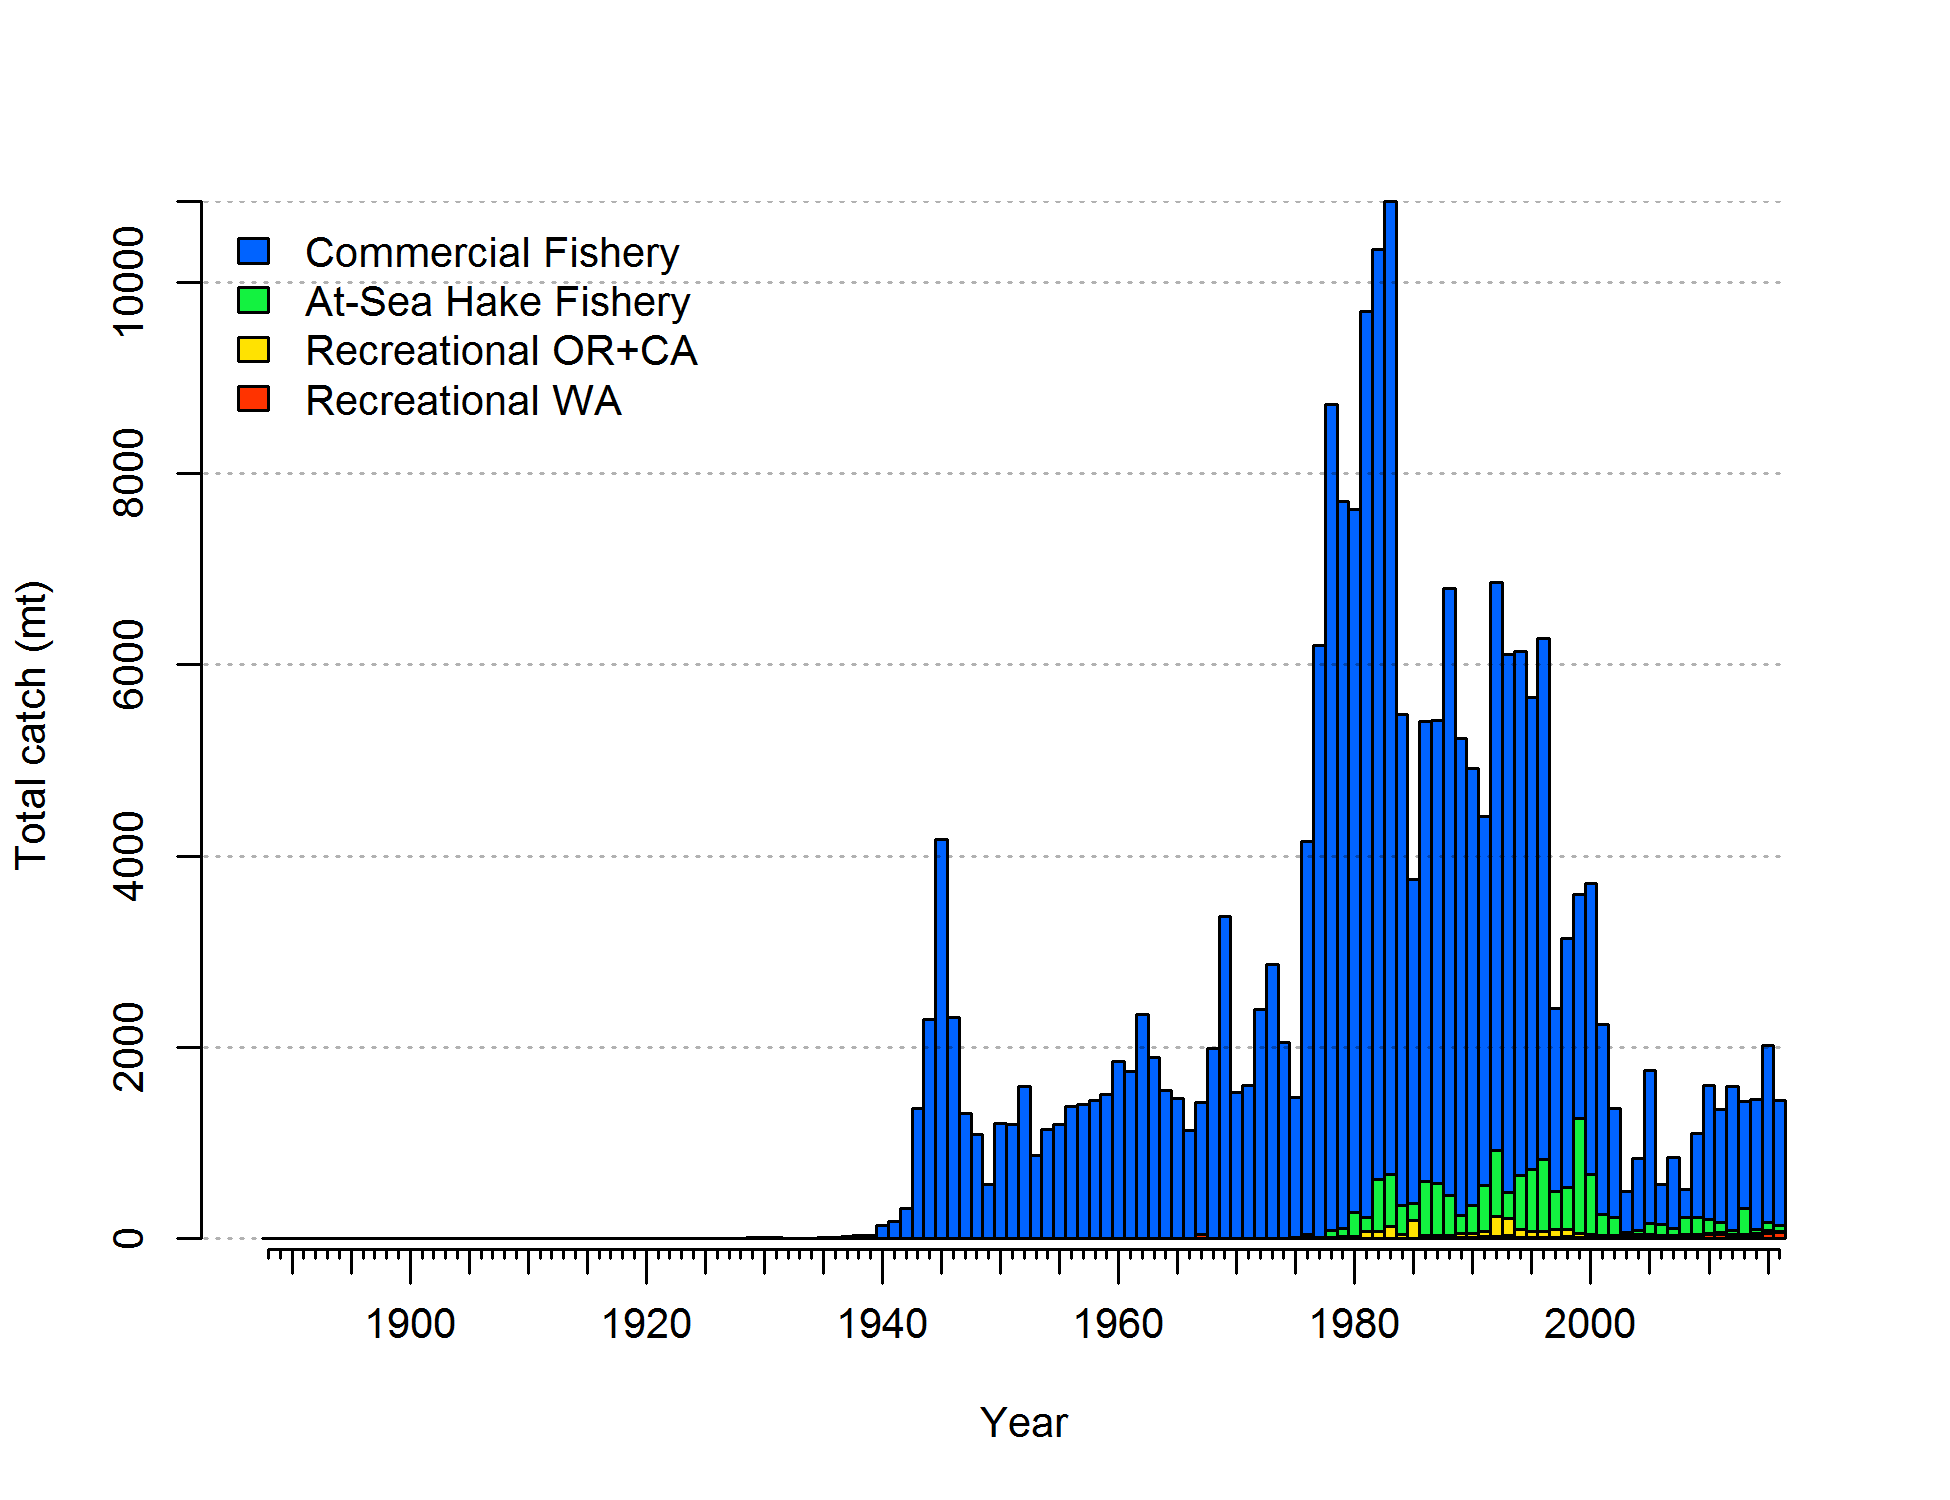
\includegraphics{r4ss/plots_mod1/catch5 total catch (including discards) stacked.png}
\caption{Estimated catch history of Yellowtail Rockfish in the Northern
model. Recreational catches in Washington are model estimates of total
weigth converted from input catch in numbers using model estimates of
growth and selectivity. Catches for the Commercial Fishery include
estimated discards.\label{fig:r4ss_total_catch_N}}
\end{figure}

\begin{figure}[htbp]
\centering
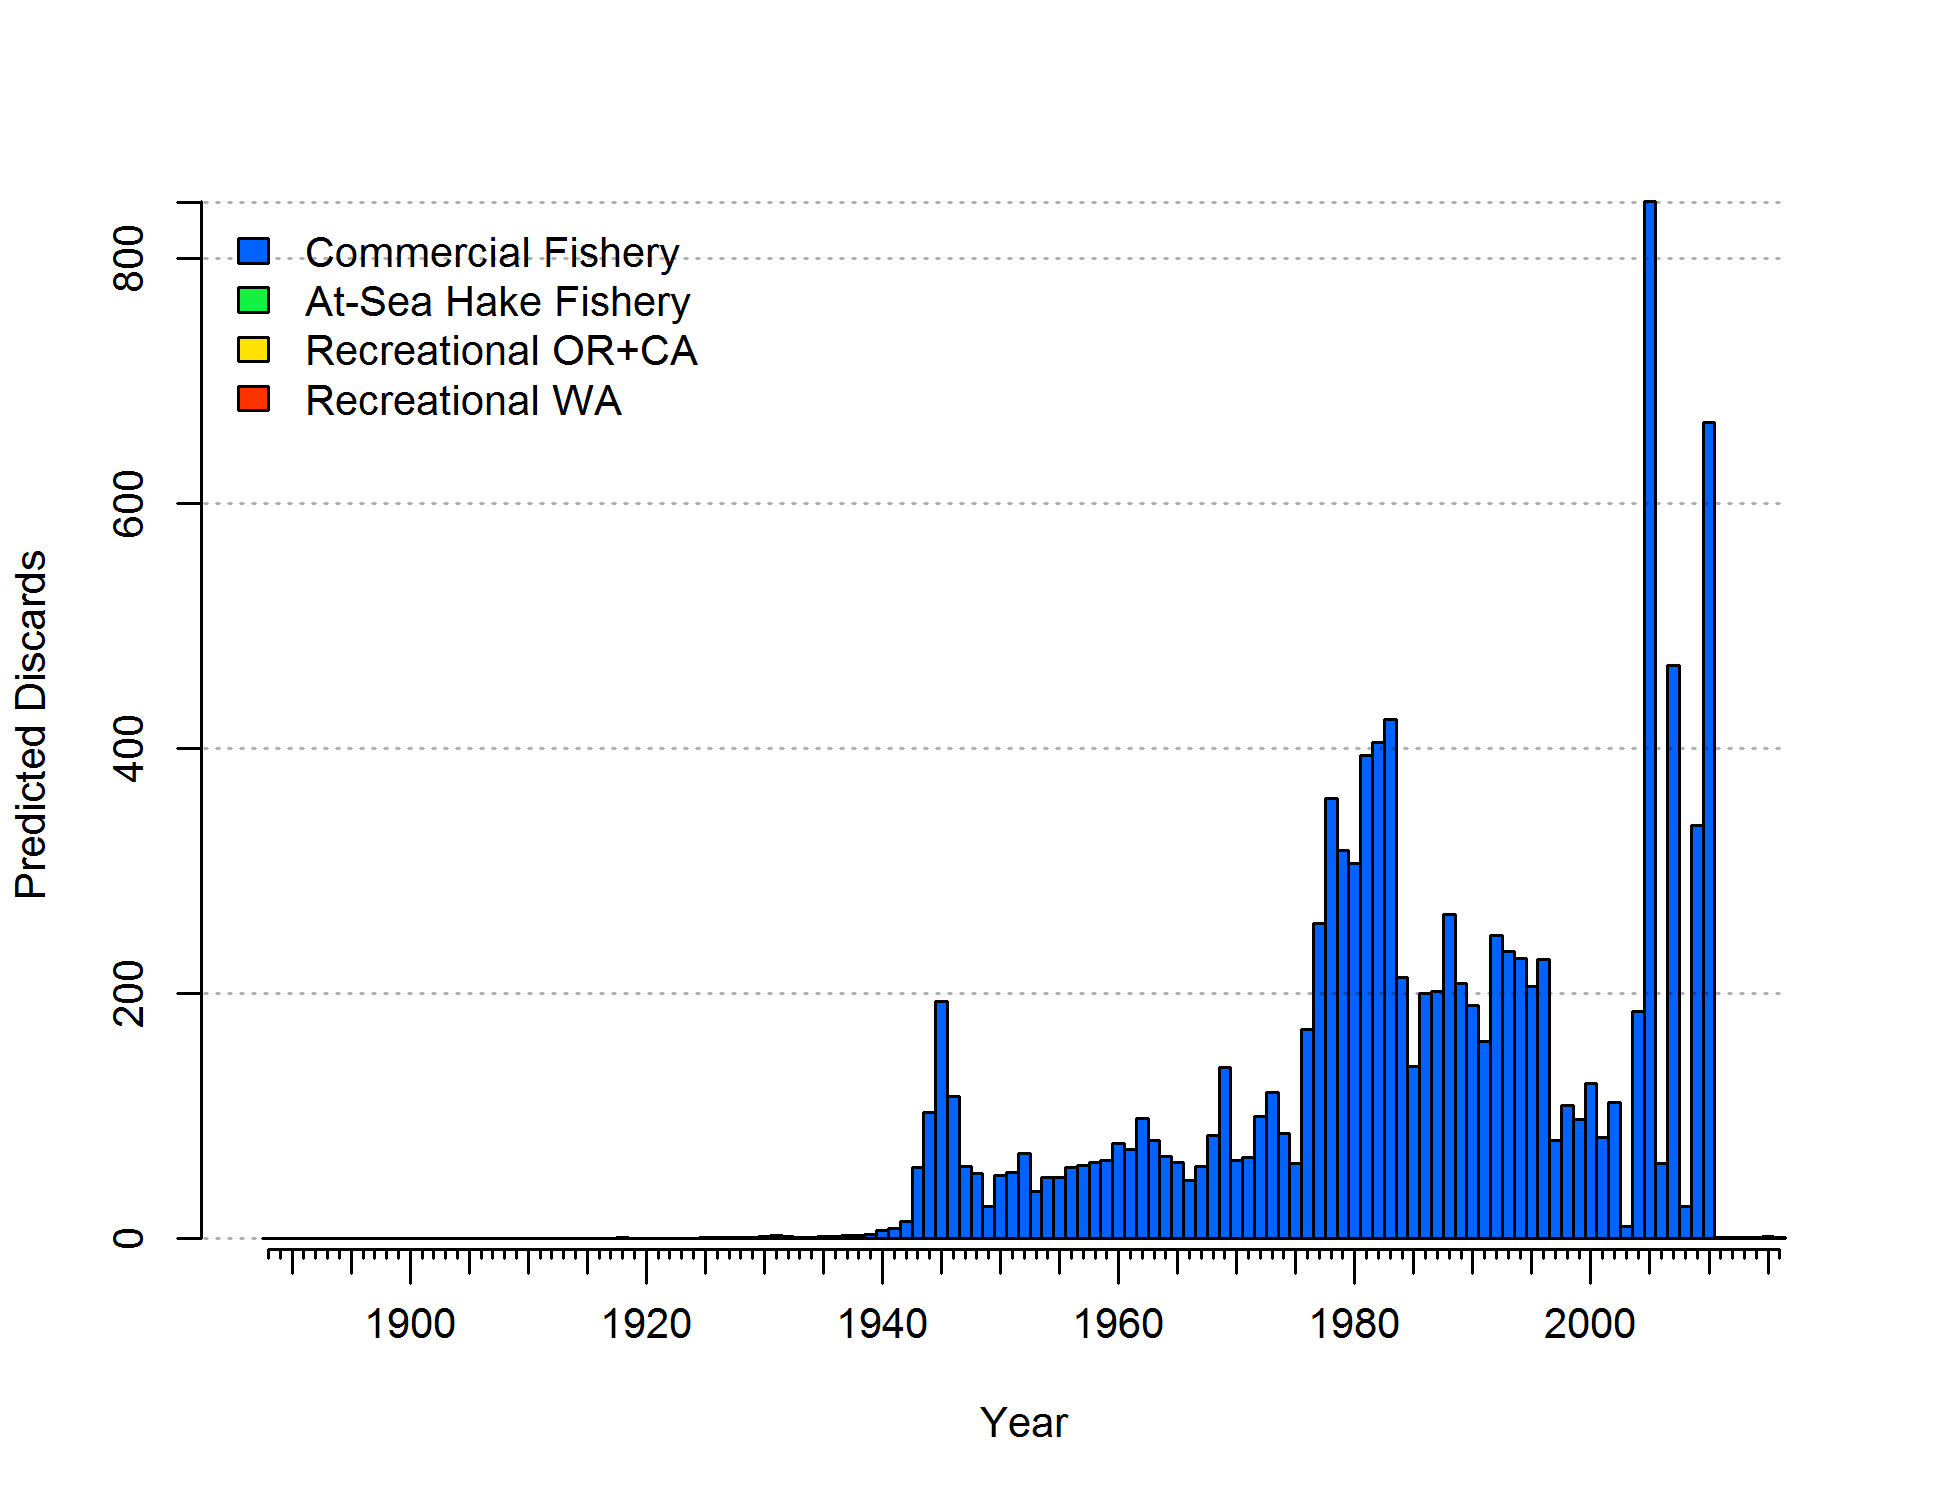
\includegraphics{r4ss/plots_mod1/catch7 discards stacked plot (depends on multiple fleets).png}
\caption{Estimated discards in the Commercial Fishery in the Northern
model. Estimates are influenced by the data for landings, discard
ratios, and discard length combines and depend on the estimated
parameters controlling selectivity and
retention.\label{fig:r4ss_discard_N}}
\end{figure}

\FloatBarrier

\begin{figure}[htbp]
\centering
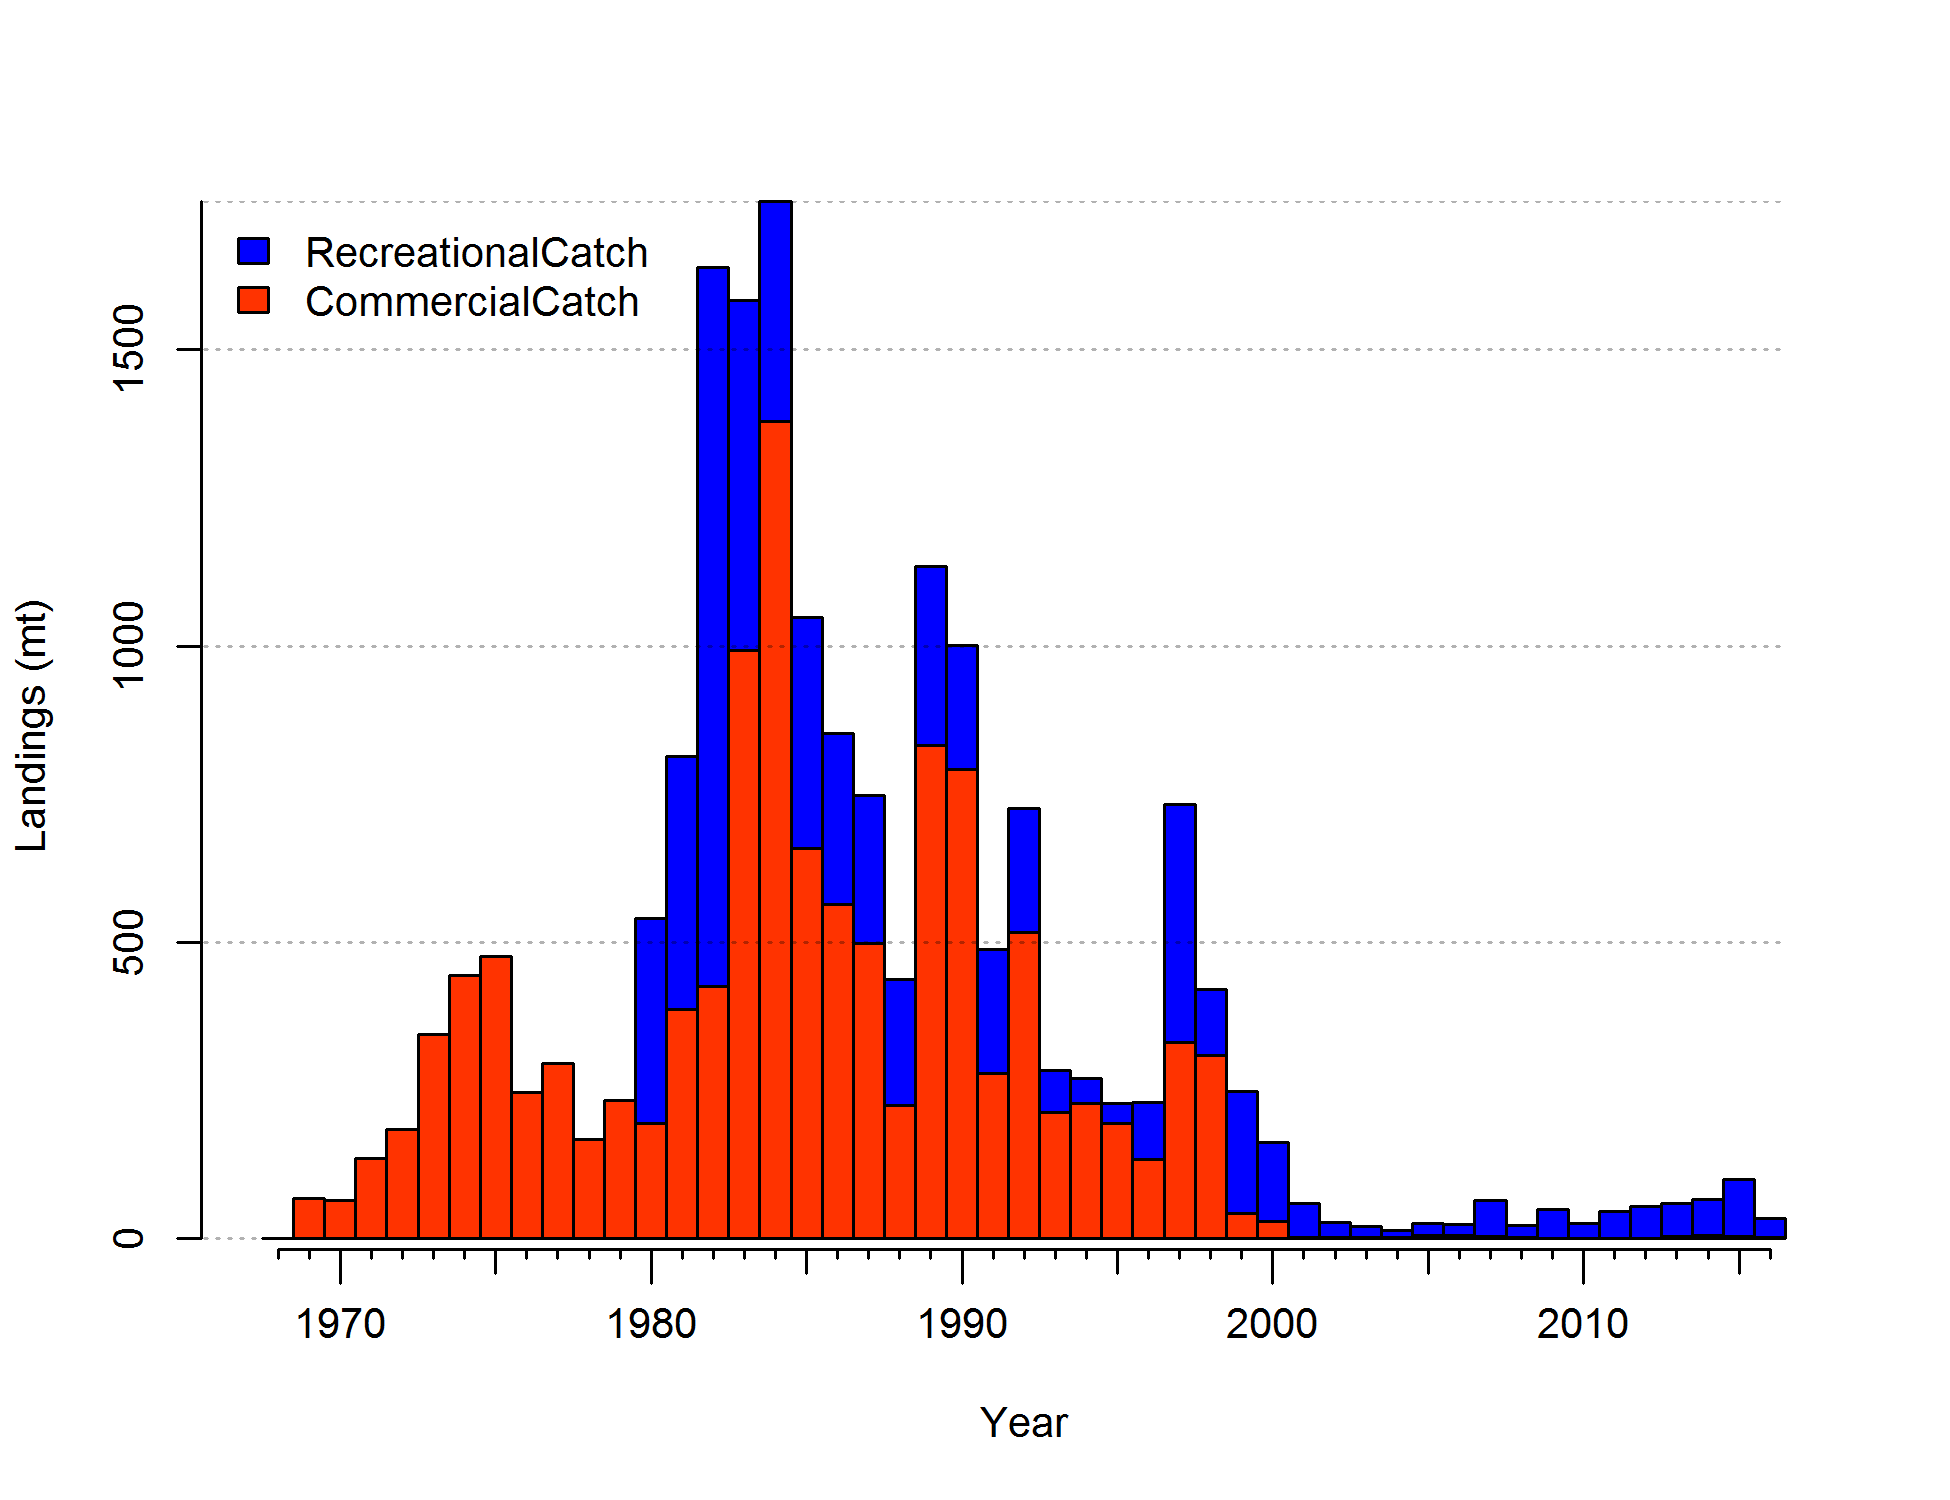
\includegraphics{r4ss/plots_mod2/catch2 landings stacked.png}
\caption{Estimated catch history of Yellowtail Rockfish in the Southern
model. \label{fig:r4ss_catch2_S}}
\end{figure}

\FloatBarrier

\newpage

\subsection{Life History (Maturity, Fecundity, Weight-Length, and
Growth)}\label{life-history-maturity-fecundity-weight-length-and-growth}

\begin{figure}[htbp]
\centering
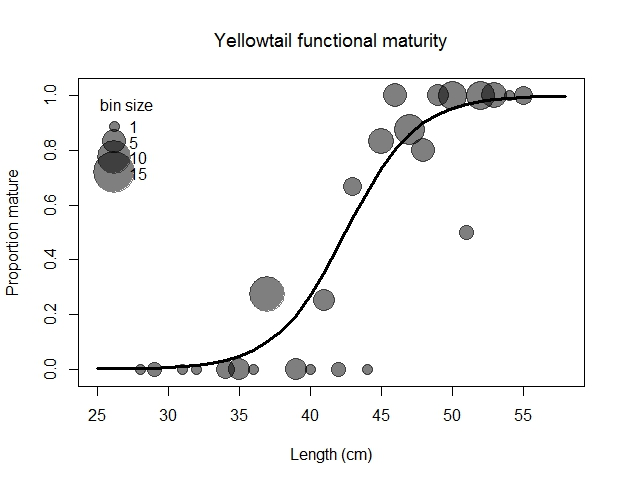
\includegraphics{Figures/YT_Propmat_update3_22.jpeg}
\caption{Estimated maturity relationship for Yellowtail Rockfish used in
both models. Gray points indicate average observed functional maturity
within each length bin with point size proportional to the number of
samples.\label{fig:maturity}}
\end{figure}

\begin{figure}[htbp]
\centering
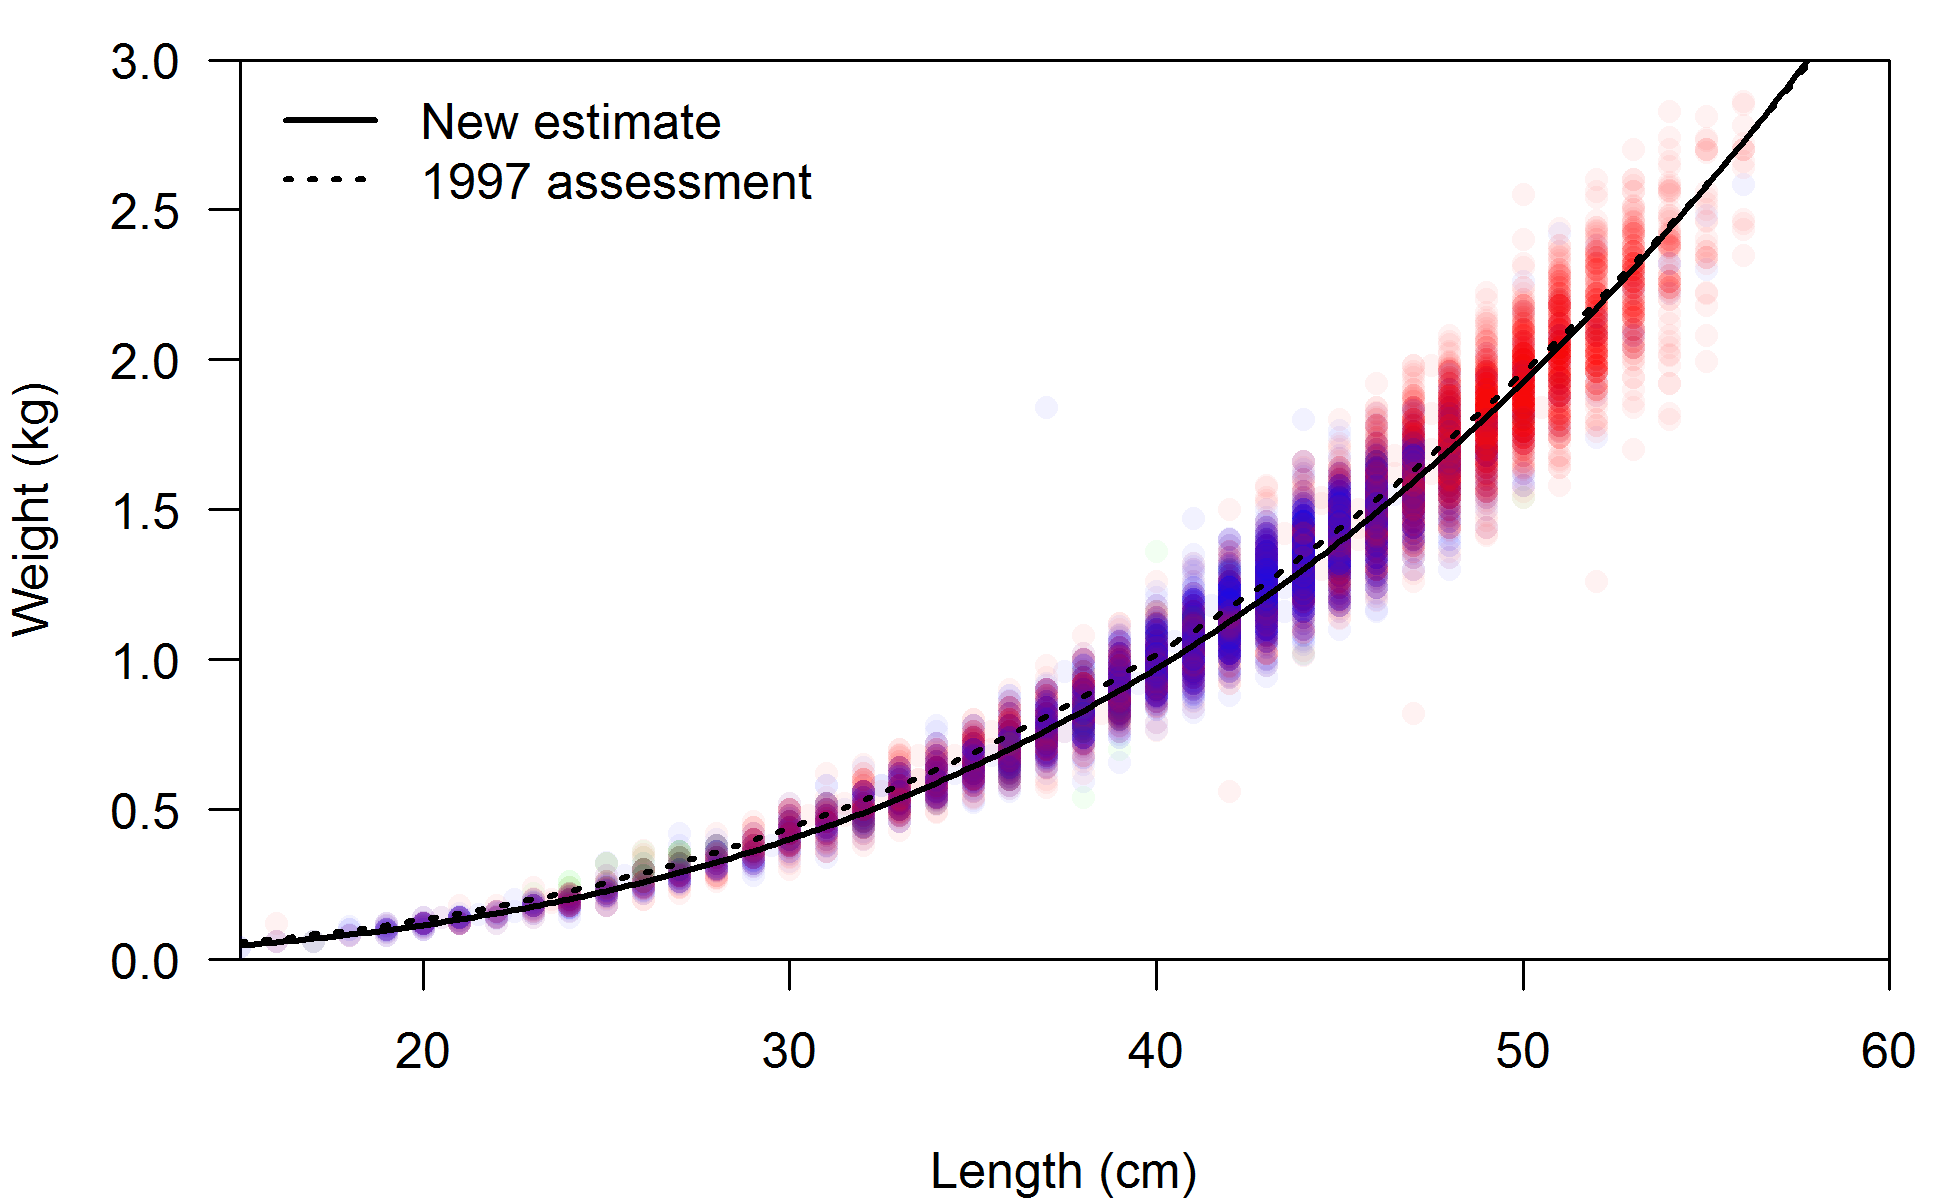
\includegraphics{Figures/weight-length_fit.png}
\caption{Estimated weight-length relationship for Yellowtail Rockfish
used in both models. Colored points show observed values (red for
females, blue for males, and green for unsexed). The black line
indicates the estimated relationship
\(W = 0.000011843L^{3.0672}\).\label{fig:weight-length}}
\end{figure}

\begin{figure}[htbp]
\centering
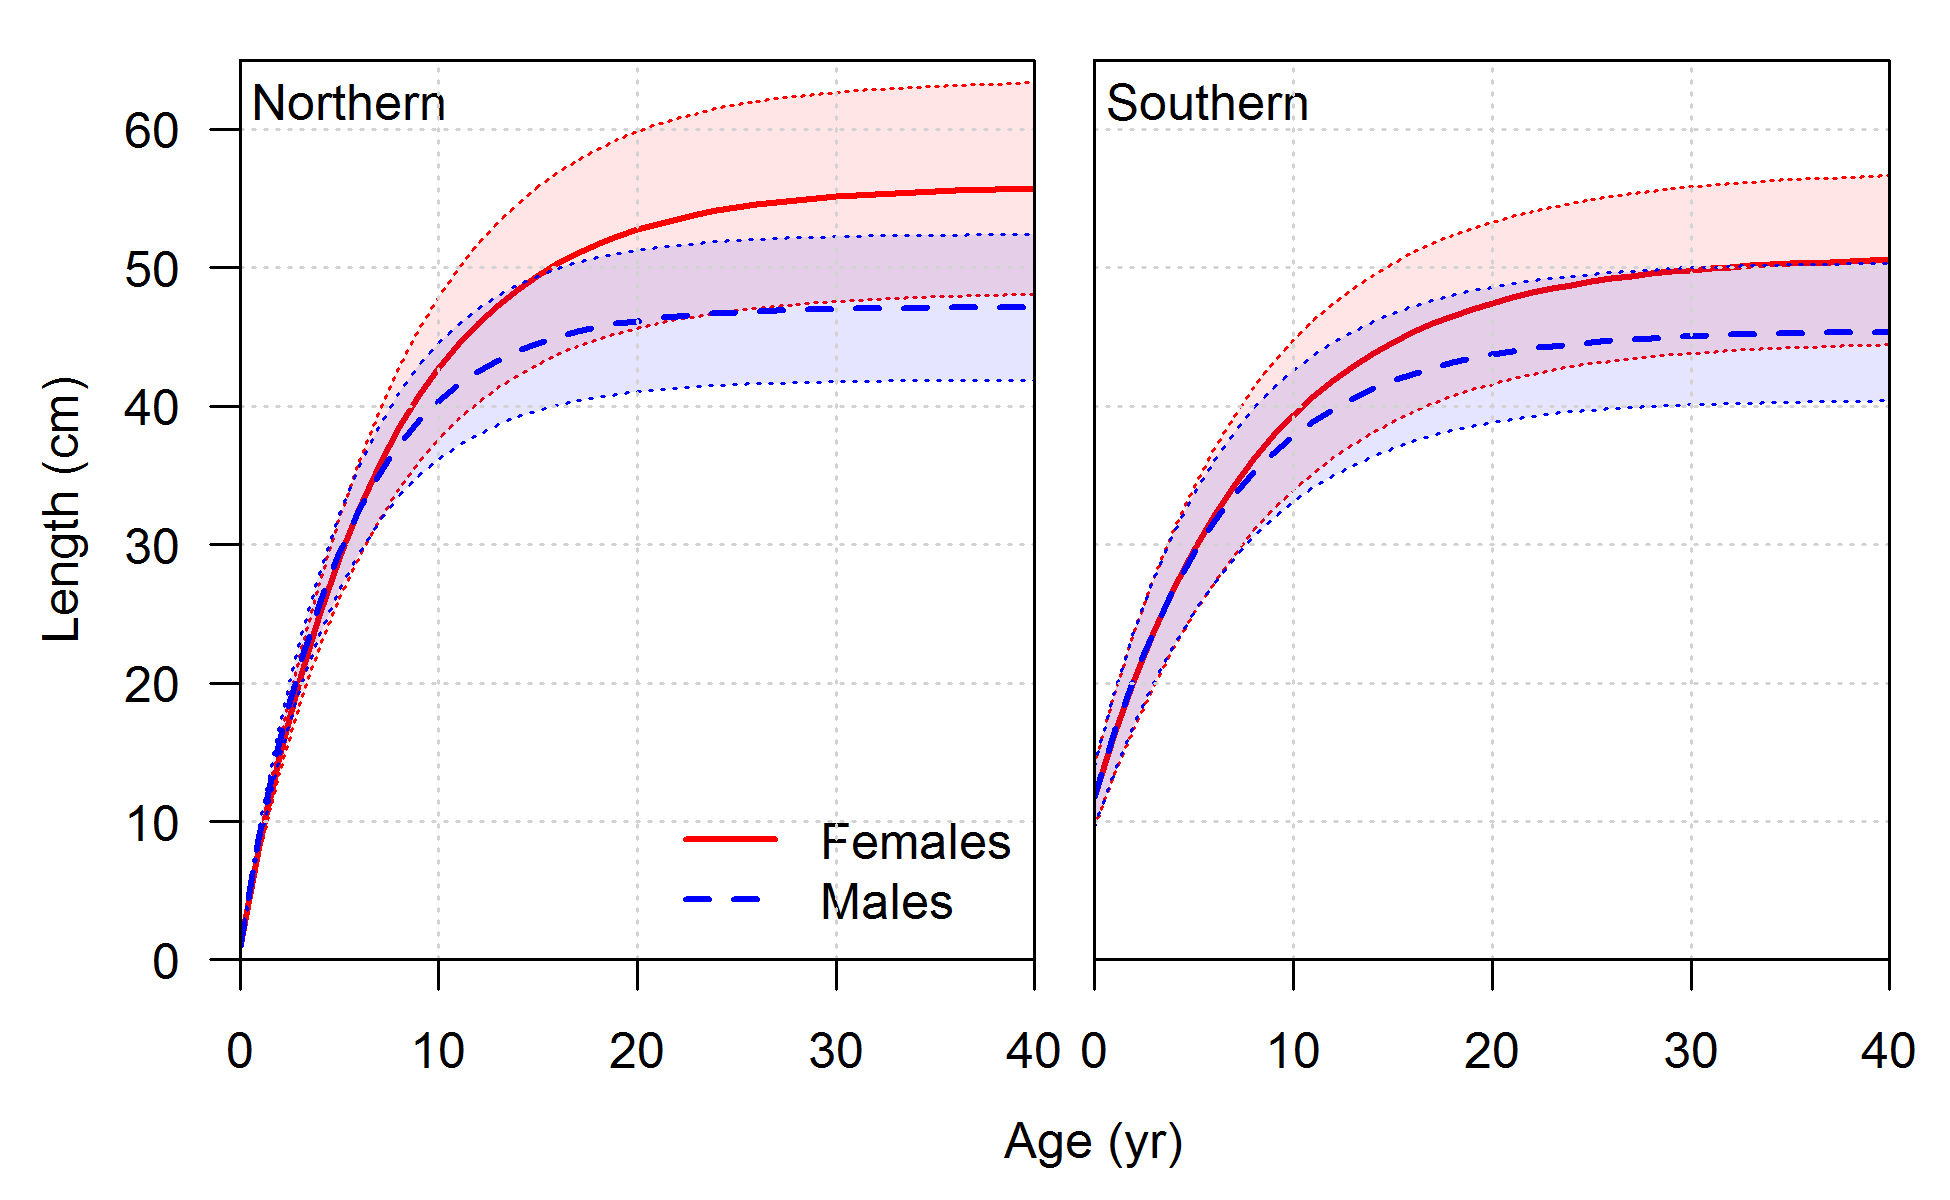
\includegraphics{r4ss/plots_compare/growth_comparison.png}
\caption{Estimated length-at-age for female and male Yellowtail Rockfish
in each model. Shaded areas indicate 95\% intervals for distribution of
lengths at each age. Values represent beginning-of-year growth.
\label{fig:growth}}
\end{figure}

\FloatBarrier 

\newpage

\subsection{Data and model fits}\label{data-and-model-fits}

\subsubsection{Data summary}\label{data-summary}

\begin{figure}[htbp]
\centering
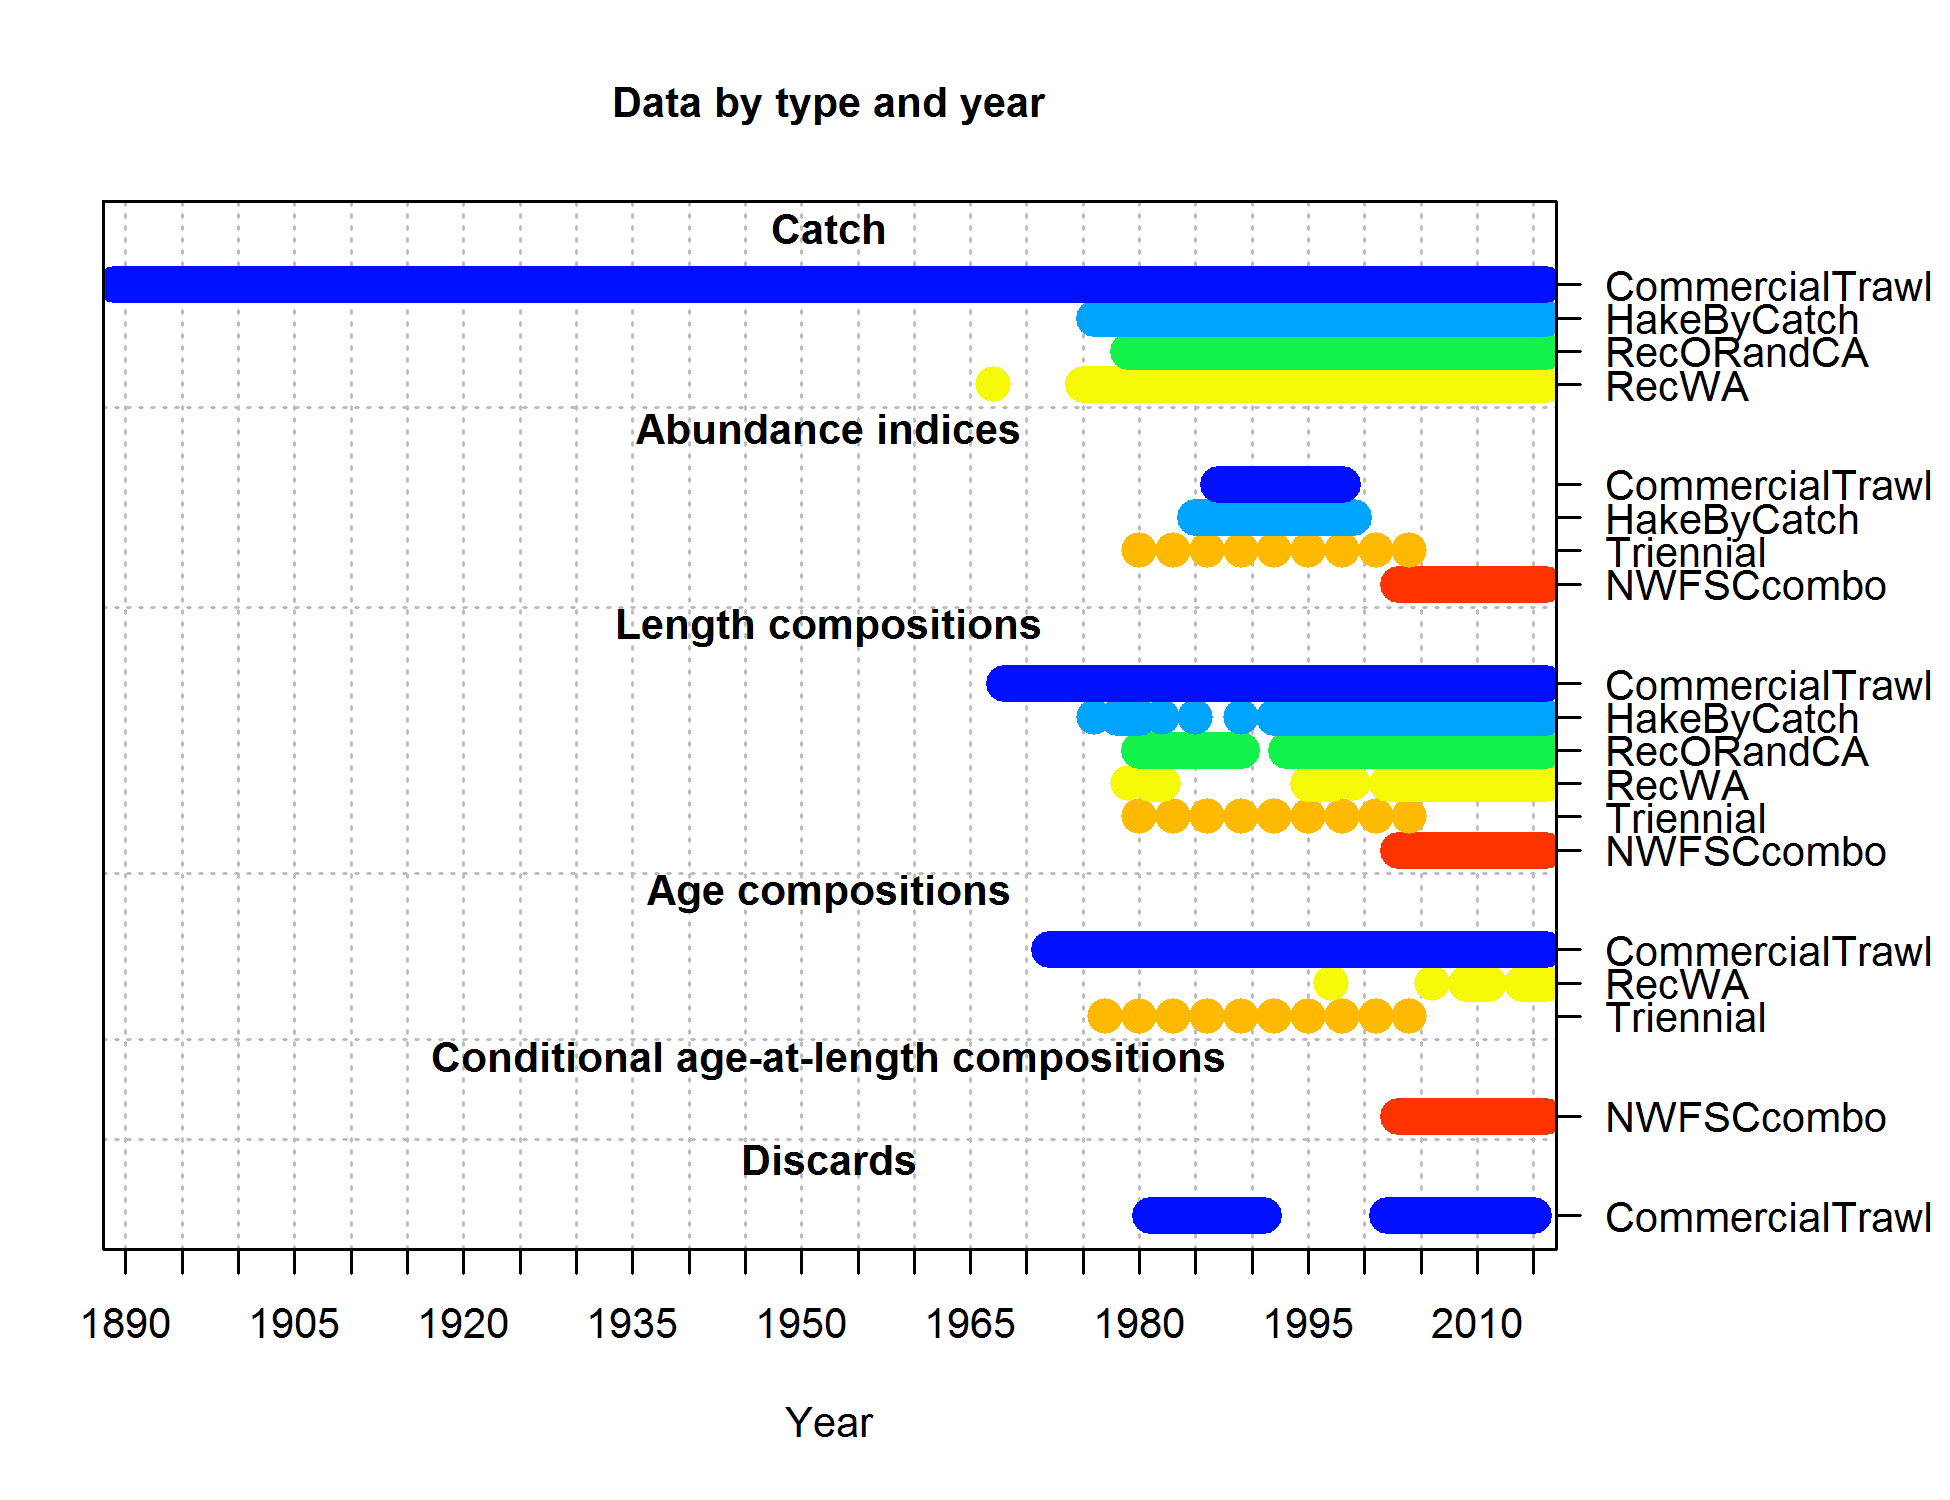
\includegraphics{r4ss/plots_mod1/data_plot.png}
\caption{Summary of data sources used in the Northern model.
\label{fig:data_plot}}
\end{figure}

\begin{figure}[htbp]
\centering
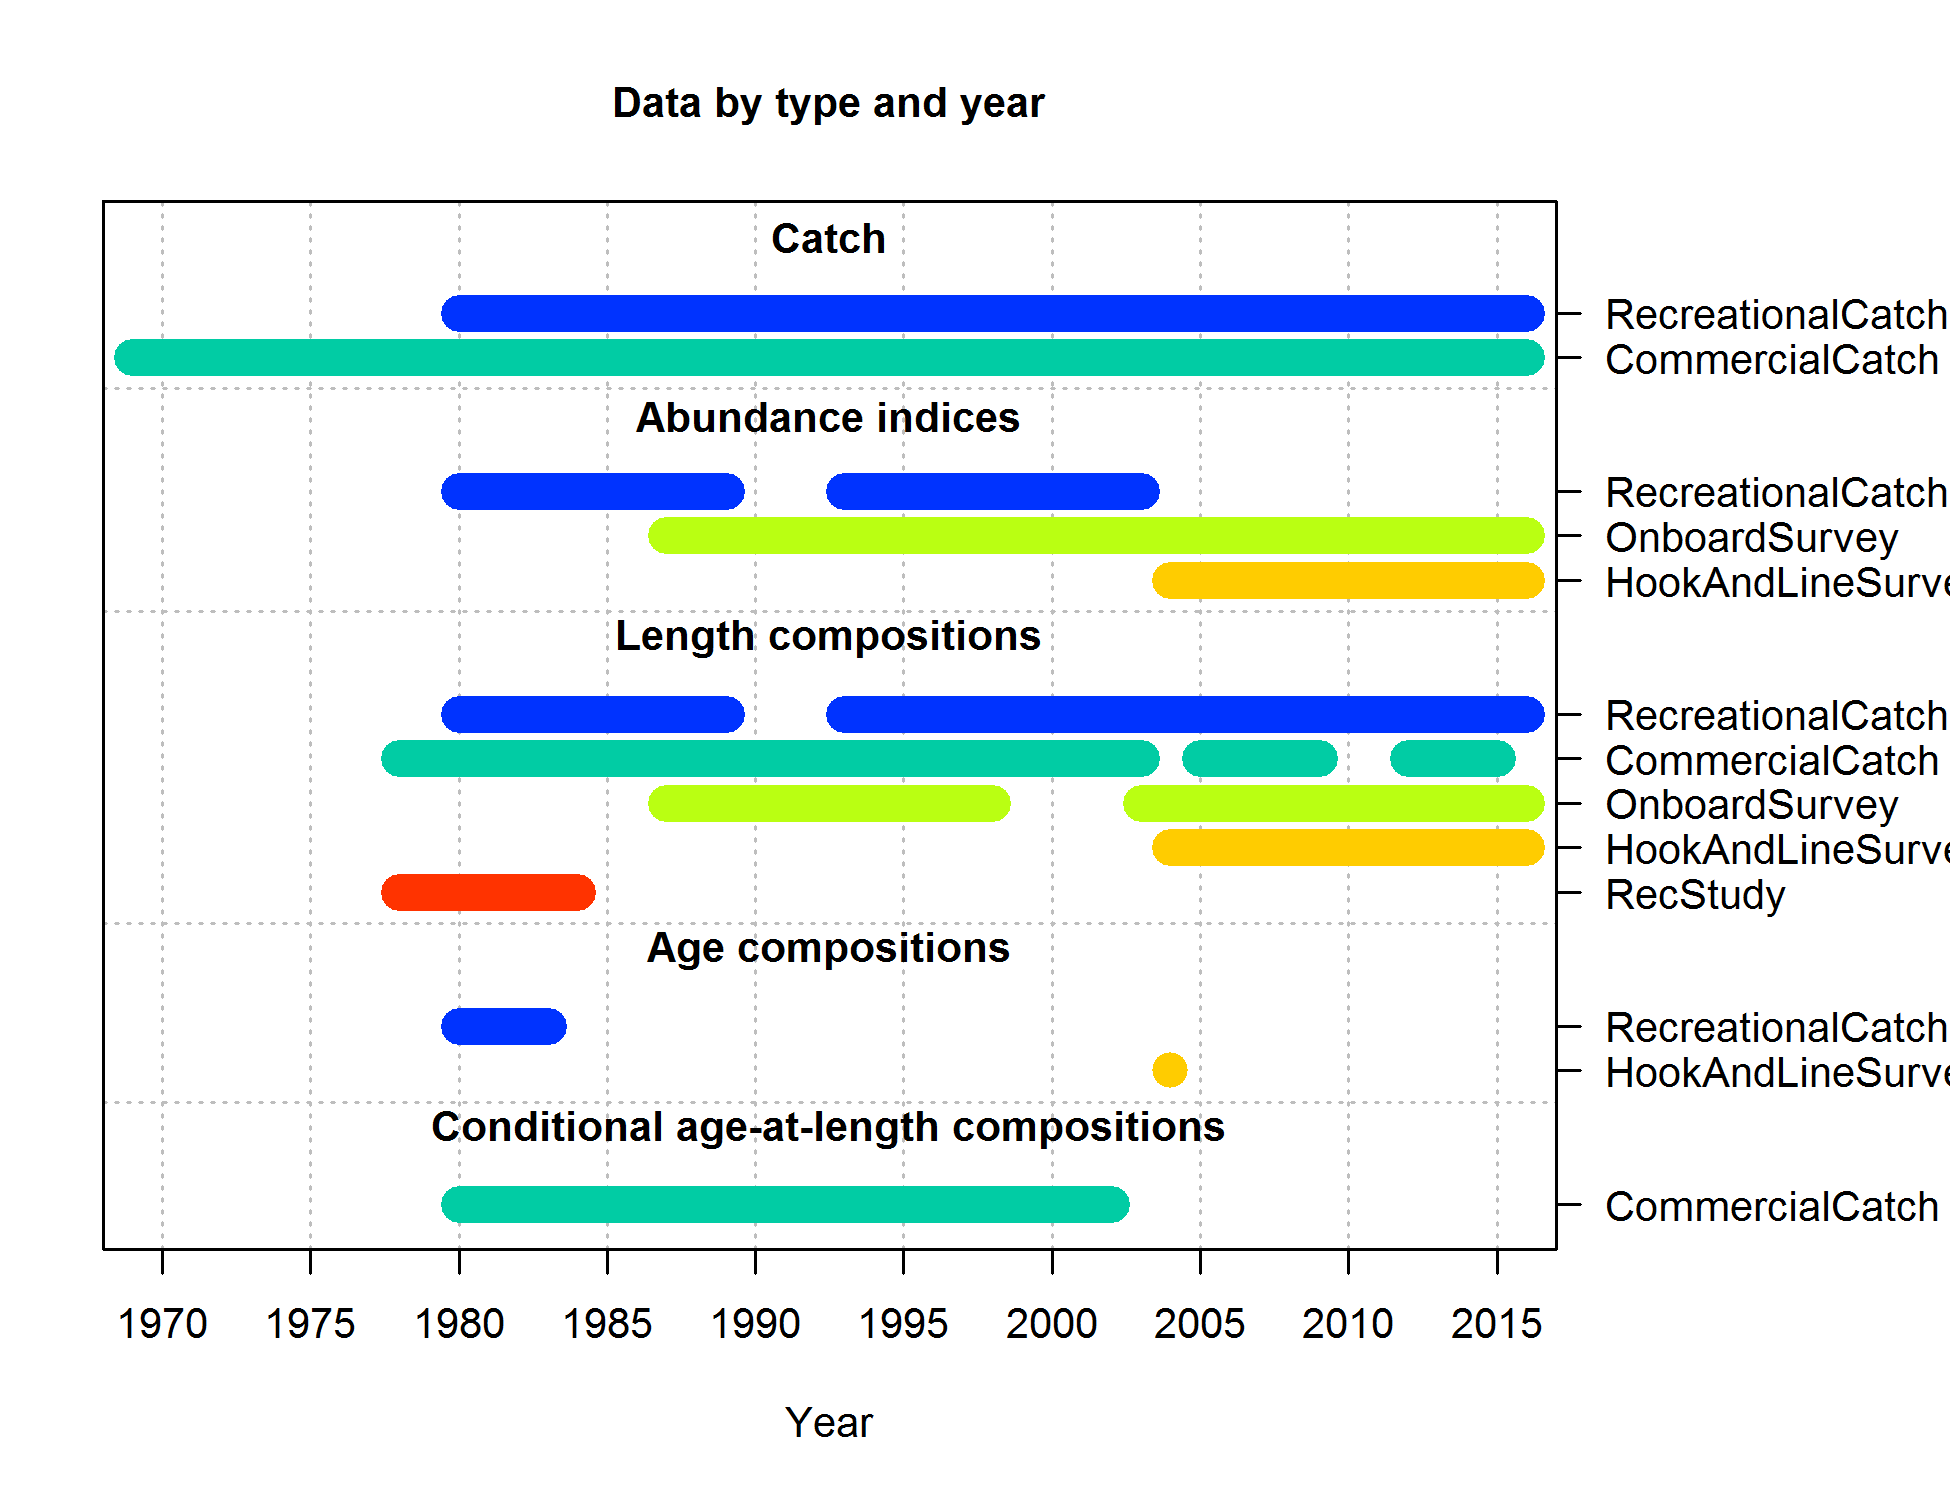
\includegraphics{r4ss/plots_mod2/data_plot.png}
\caption{Summary of data sources used in the Southern model.
\label{fig:data_plot}}
\end{figure}

\FloatBarrier

\subsubsection{Selectivity, retention, and
discards}\label{selectivity-retention-and-discards}

\begin{figure}[htbp]
\centering
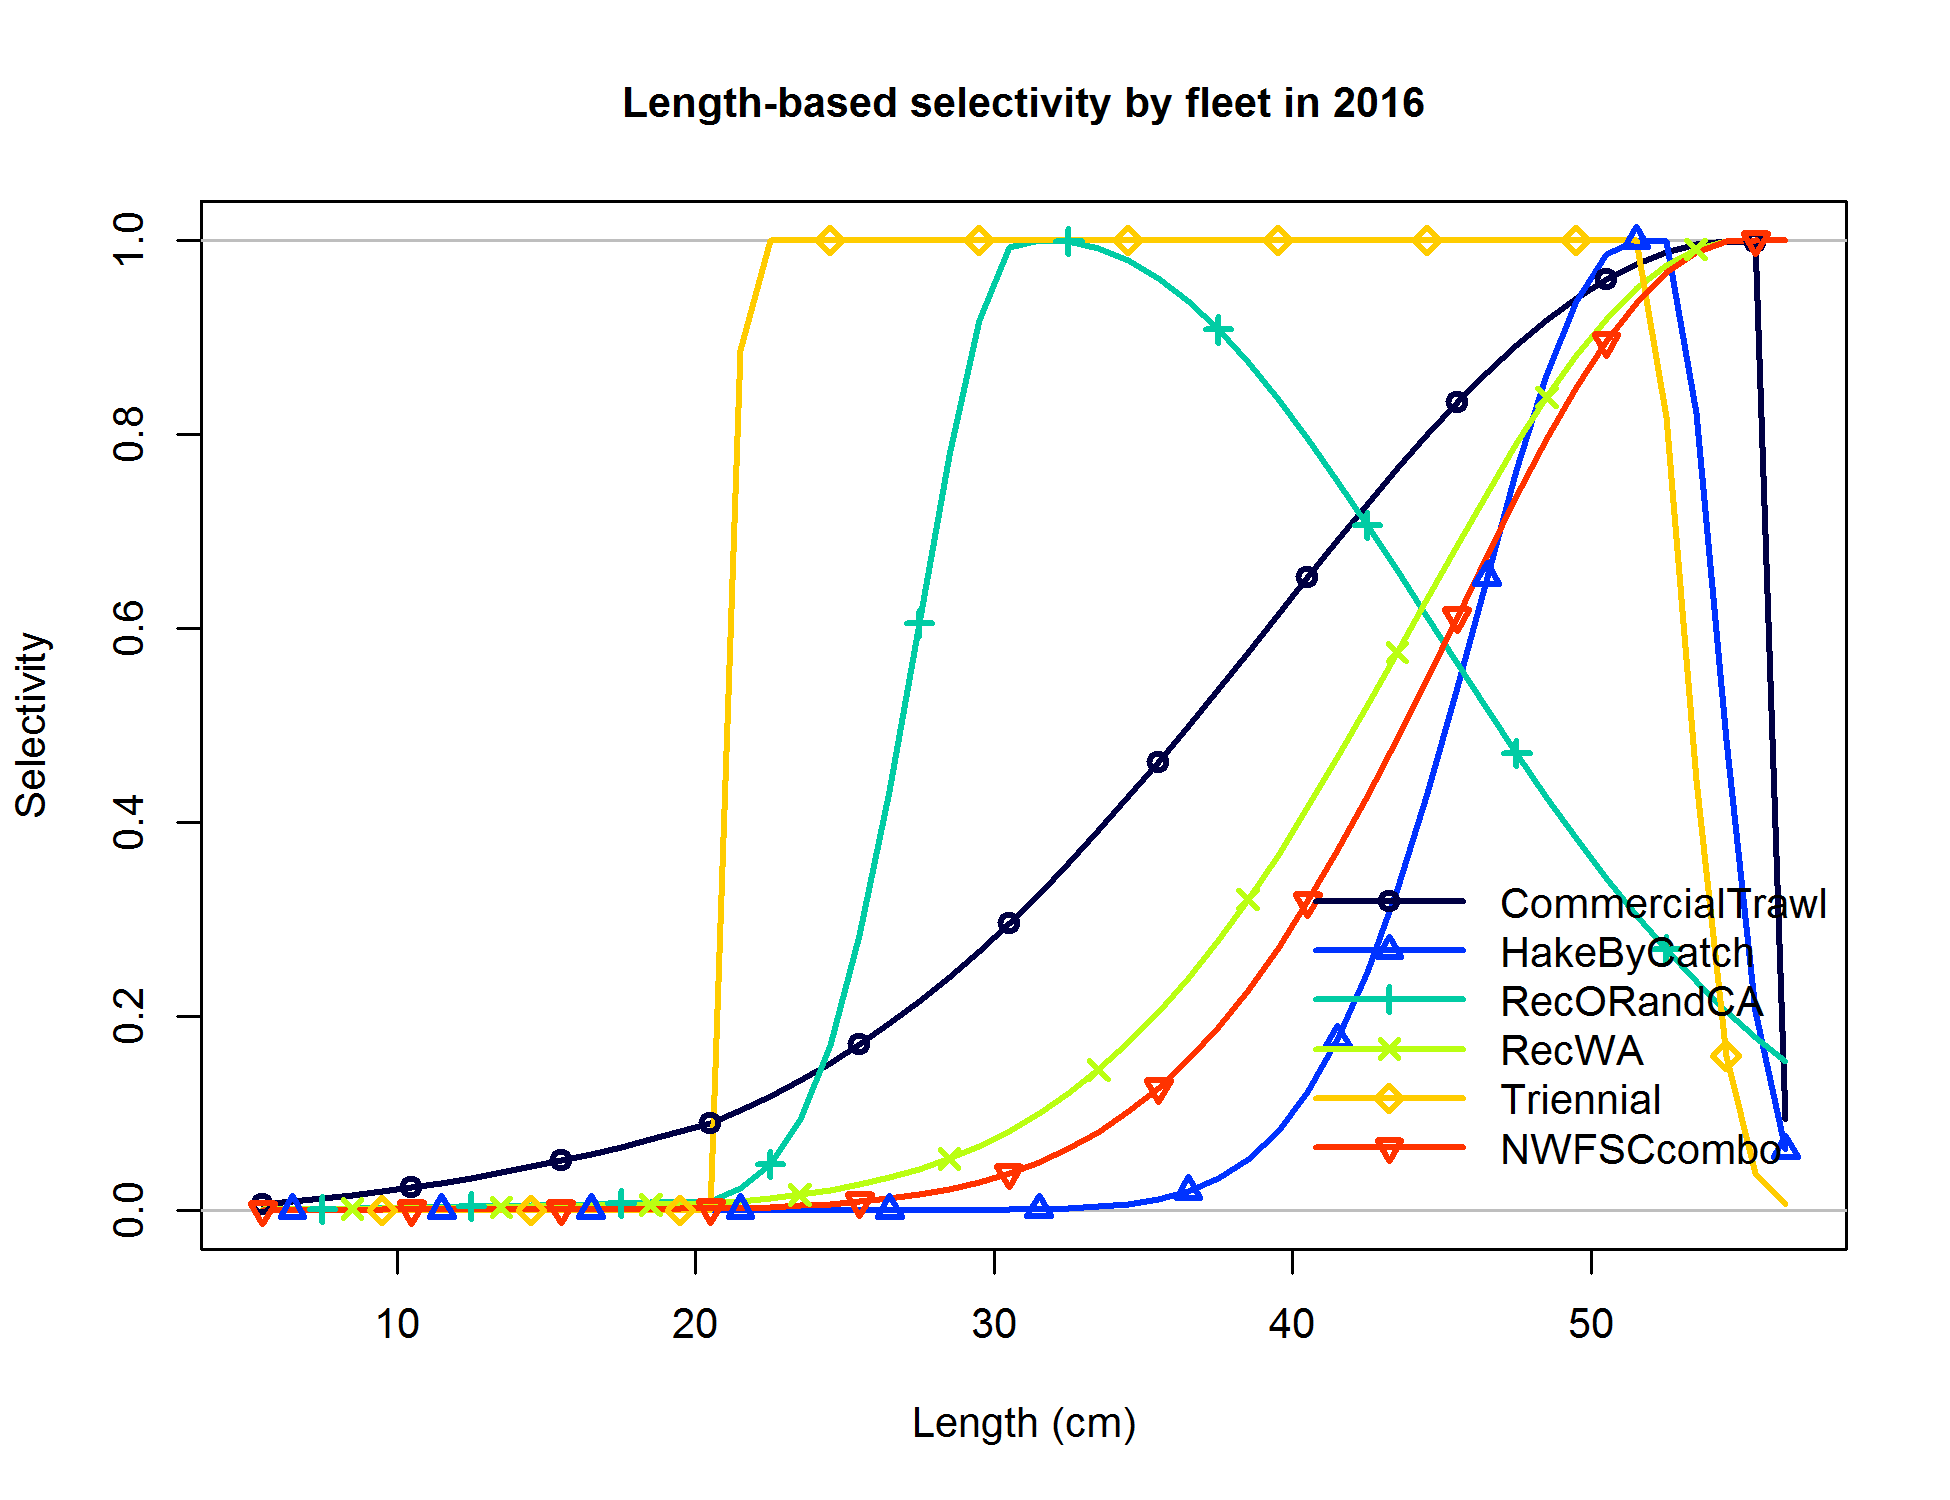
\includegraphics{r4ss/plots_mod1/sel01_multiple_fleets_length1.png}
\caption{Estimated selectivity by length by each fishery and survey in
the Northern model. \label{fig:selex}}
\end{figure}

\begin{figure}[htbp]
\centering
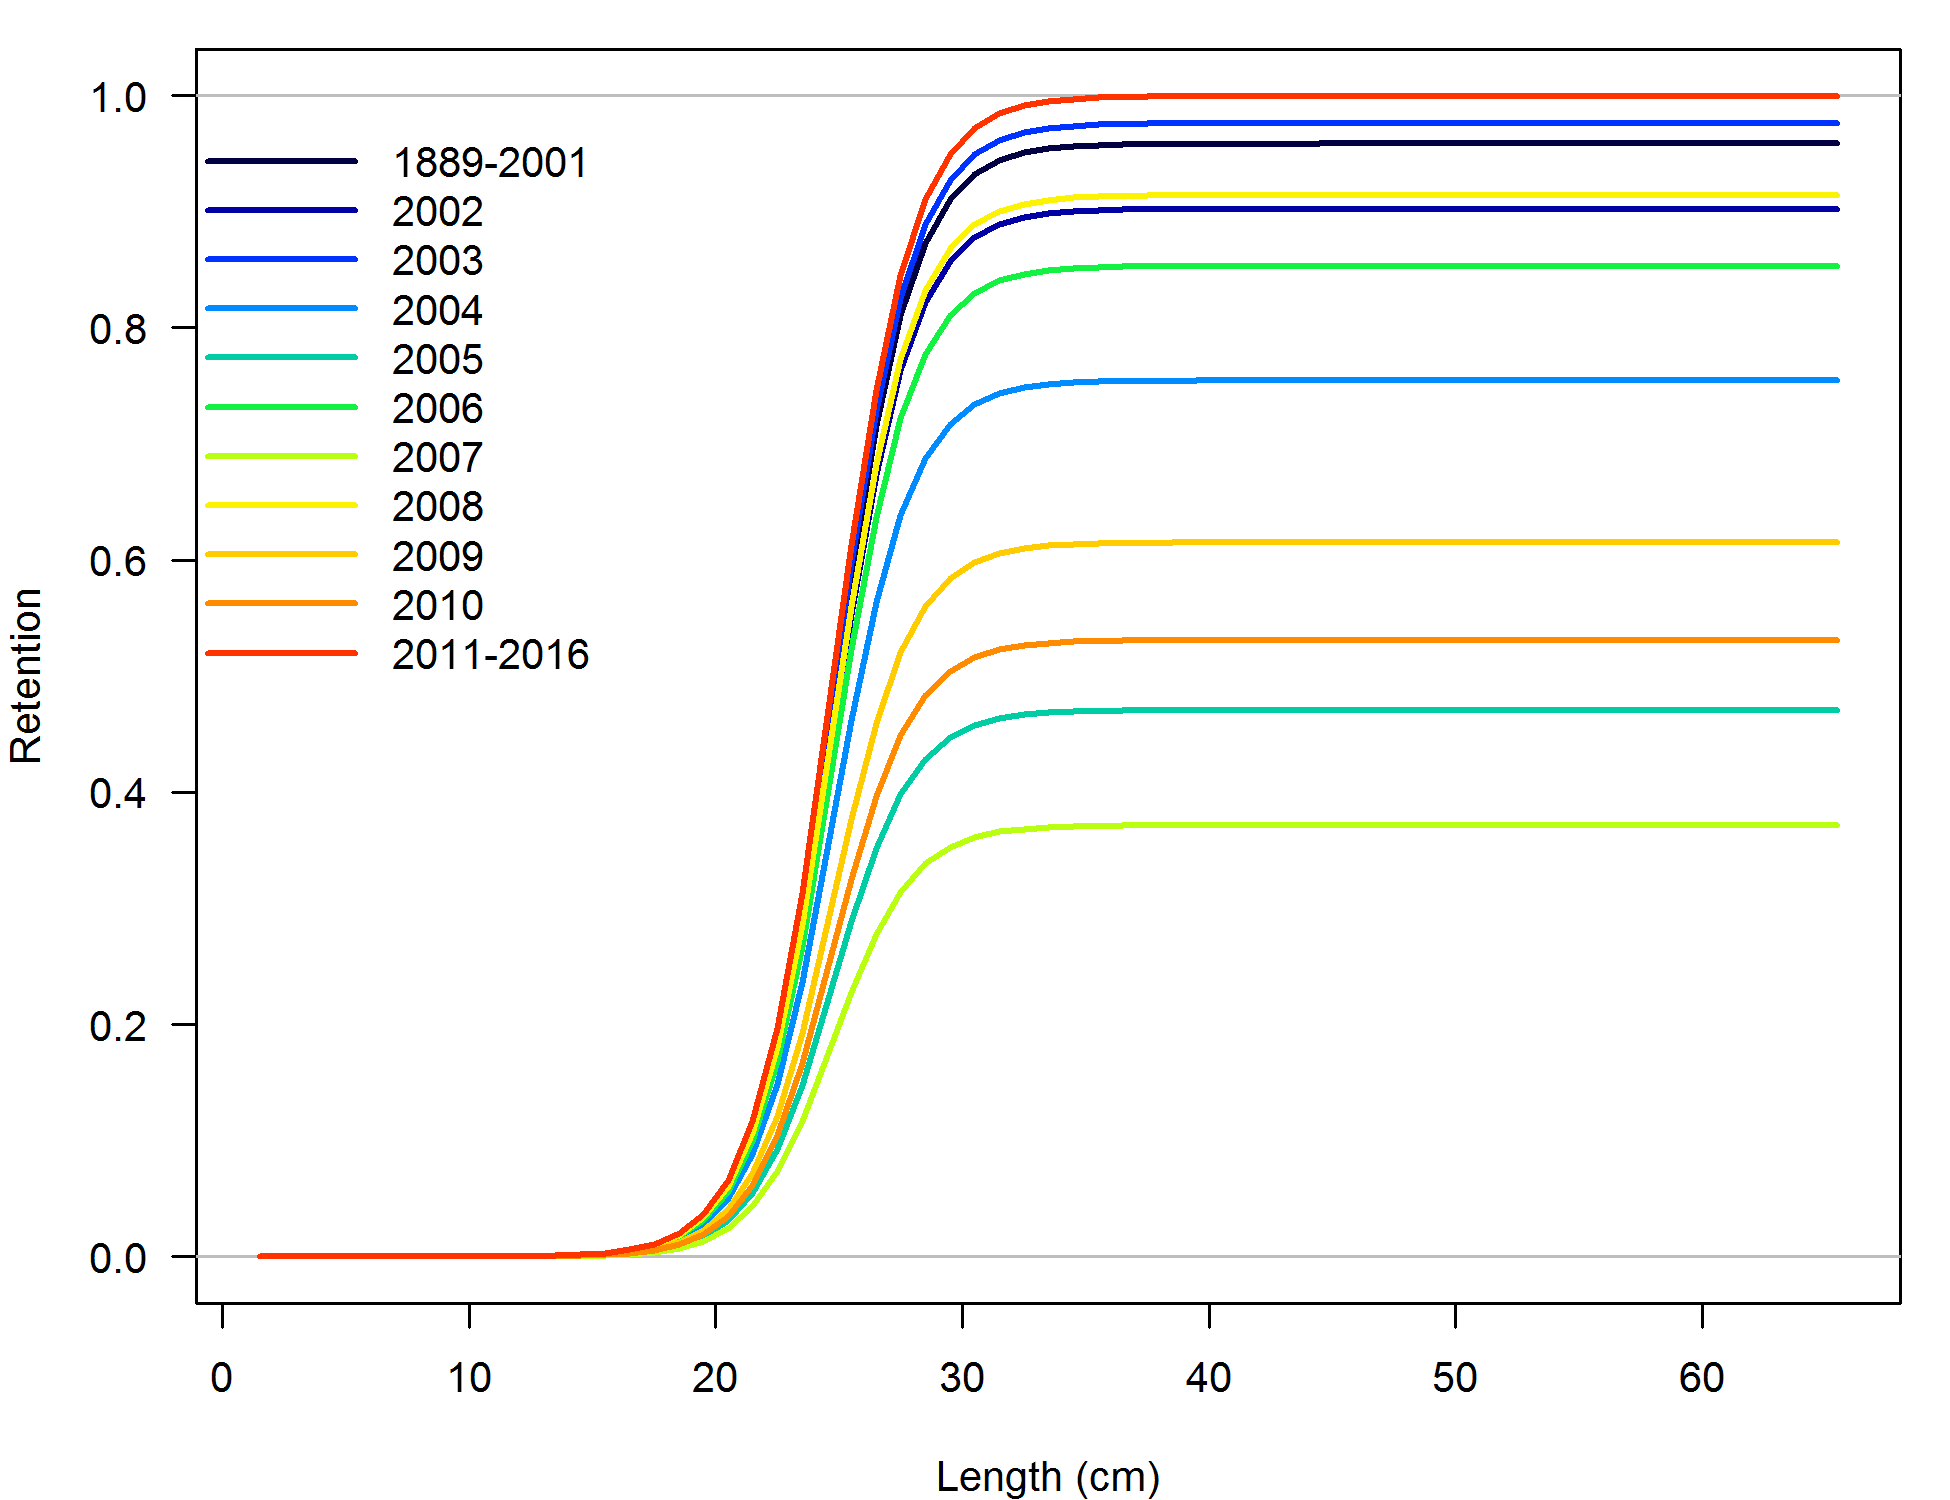
\includegraphics{r4ss/plots_mod1/time-varying_retention.png}
\caption{Estimated retention by length by the Commercial Fishery in the
Northern model. \label{fig:retention}}
\end{figure}

\begin{figure}[htbp]
\centering
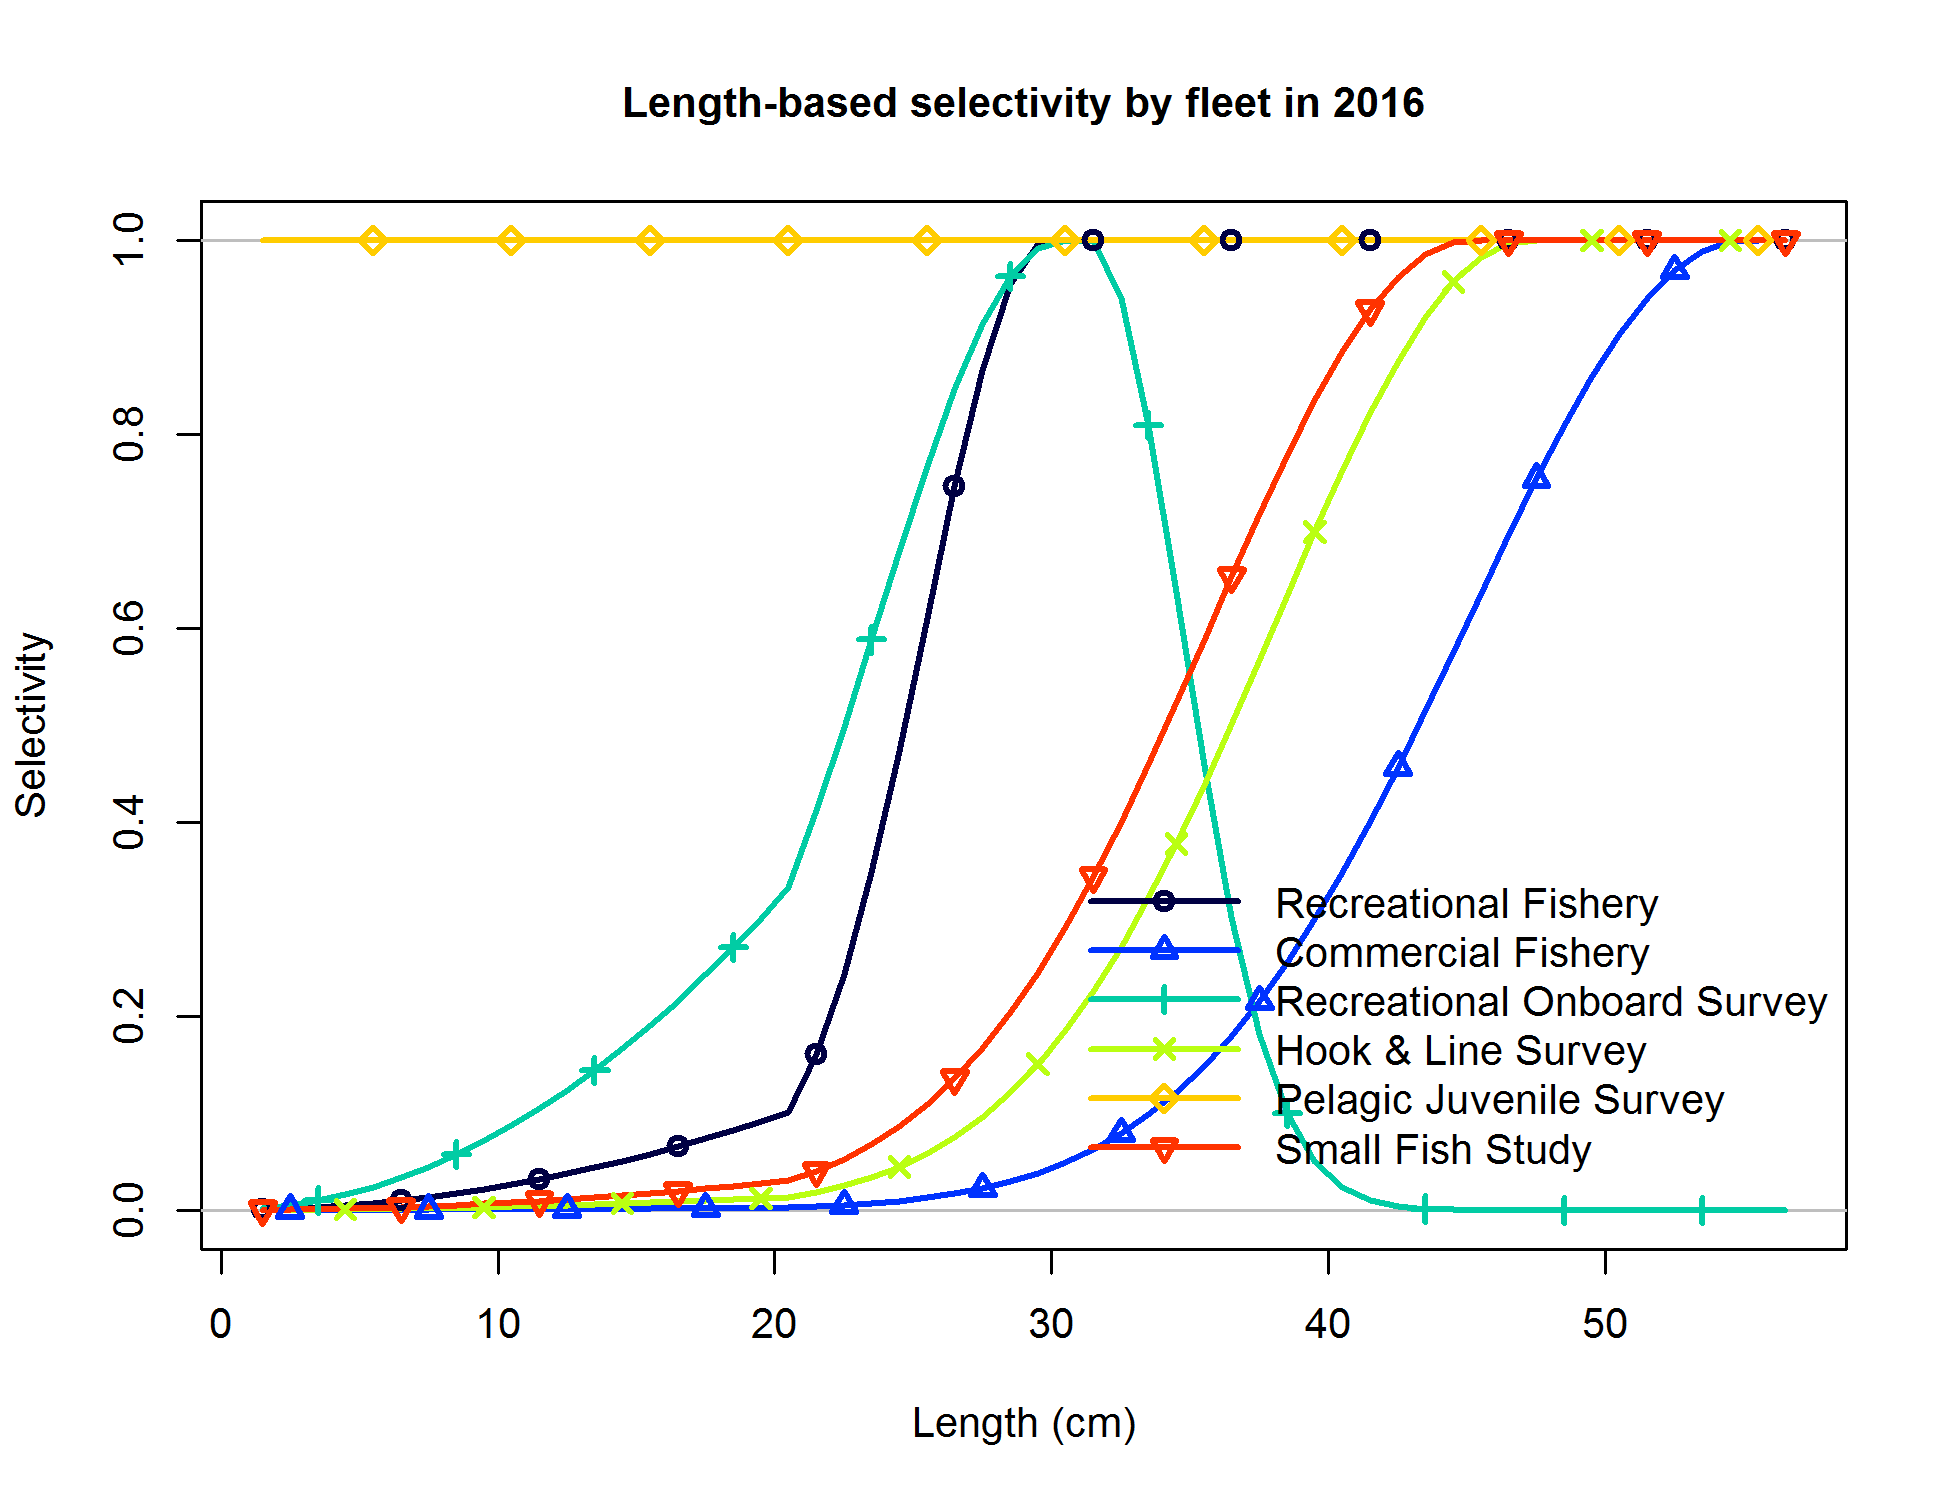
\includegraphics{r4ss/plots_mod2/sel01_multiple_fleets_length1.png}
\caption{Estimated selectivity by length by each fishery and survey in
the Southern model. \label{fig:selex}}
\end{figure}

\FloatBarrier 

\newpage

\begin{figure}[htbp]
\centering
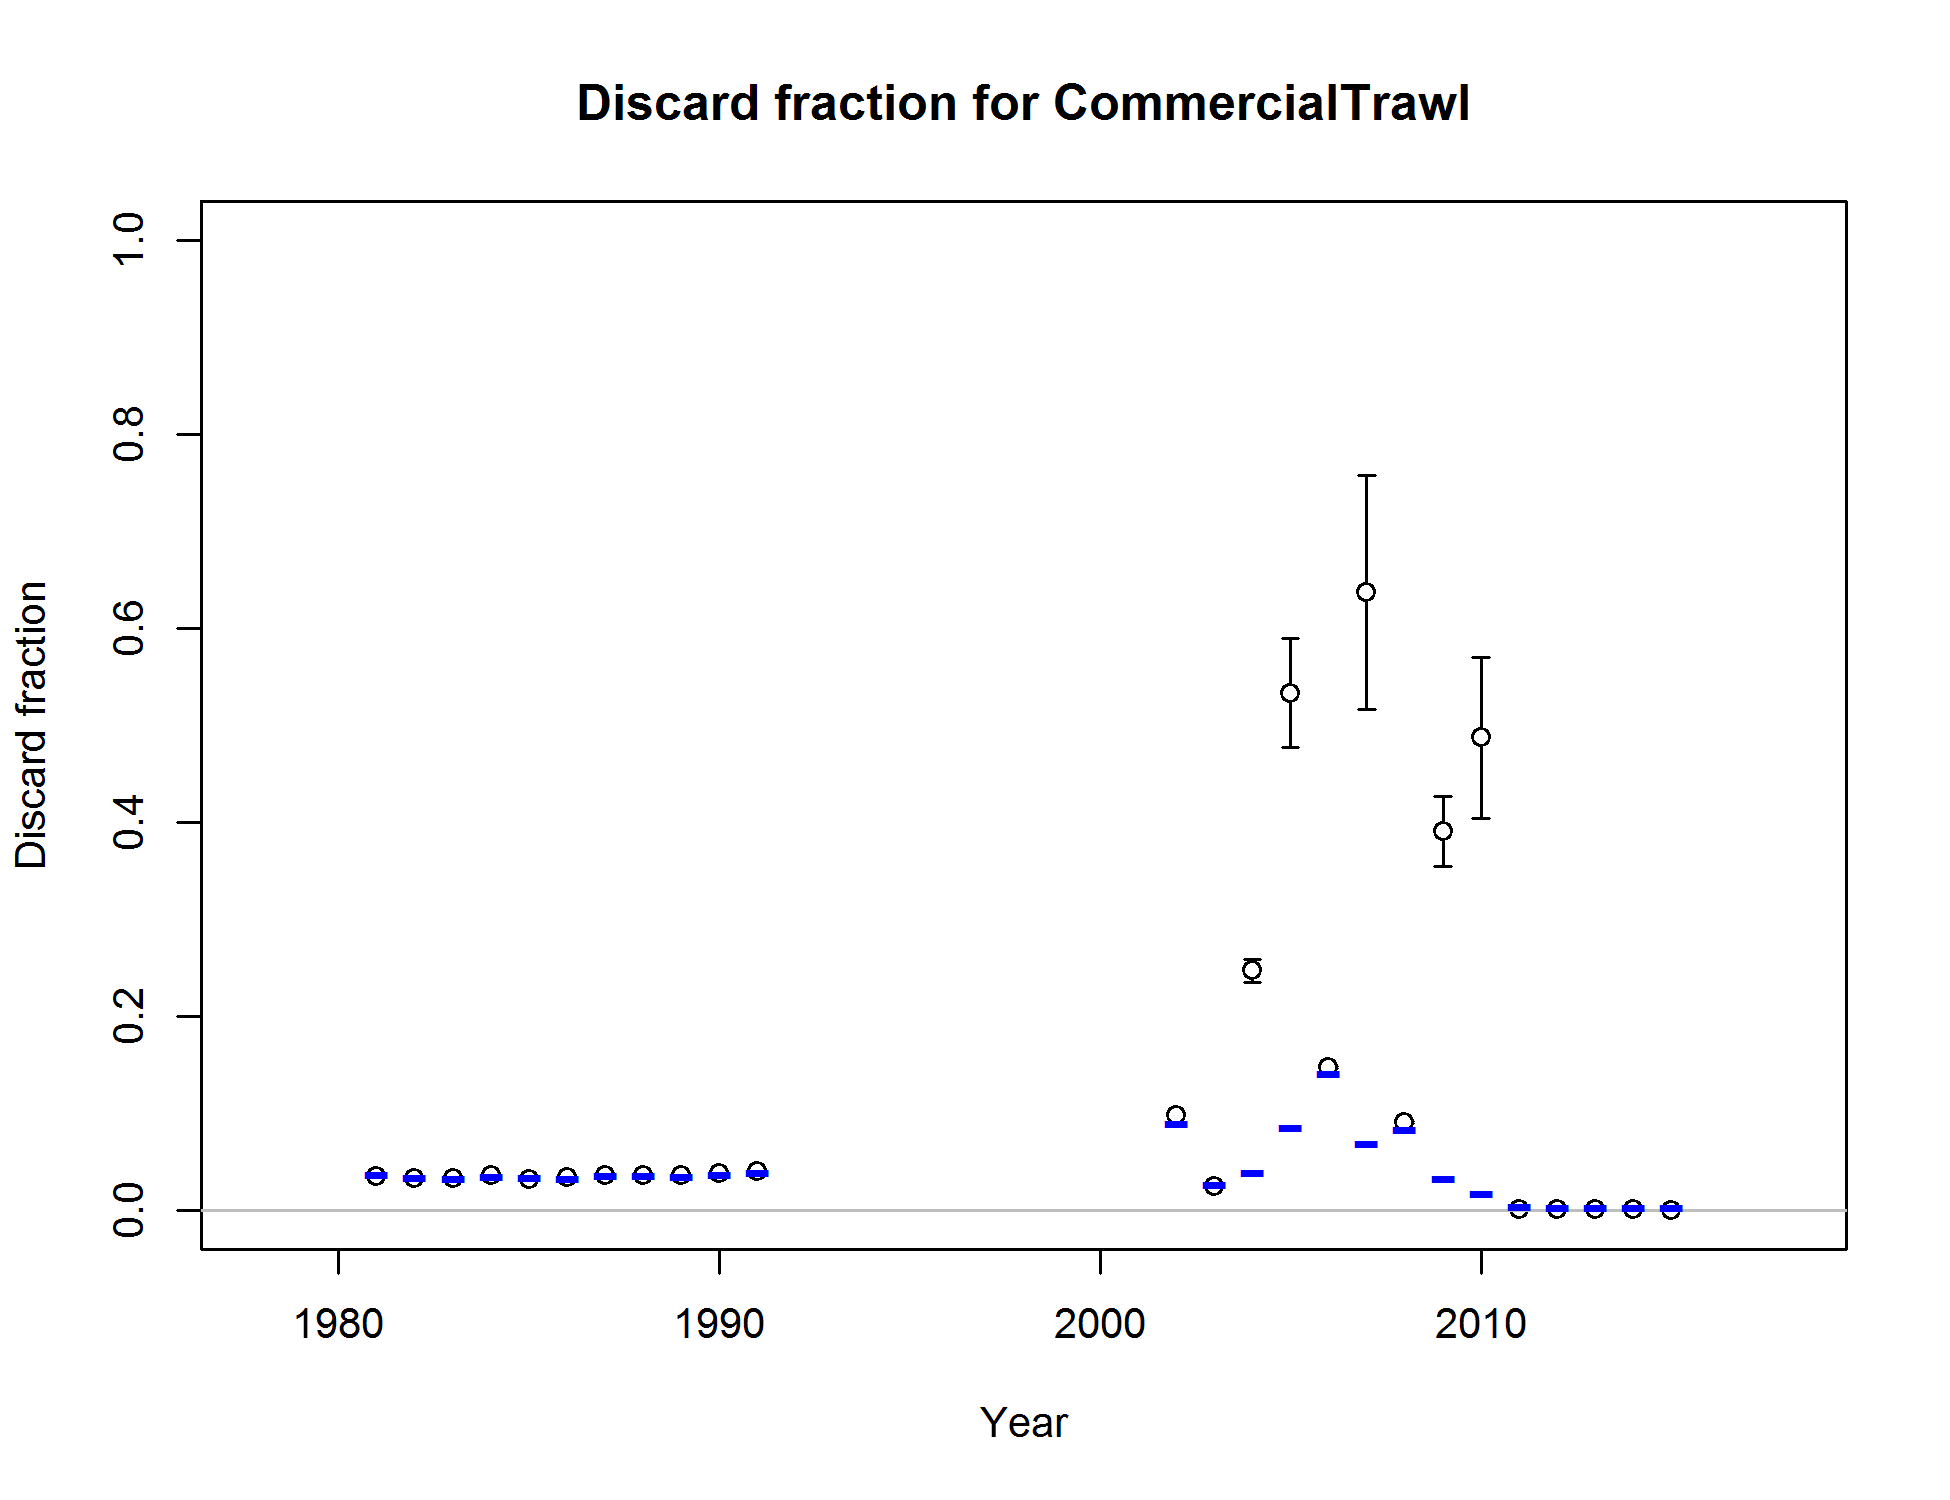
\includegraphics{r4ss/plots_mod1/discard_dataCommercialTrawl.png}
\caption{Fit to discard fractions for the commercial fishery in the
Northern model.\label{fig:r4ss_discard_fits}}
\end{figure}

\newpage

\subsubsection{Fits to indices of
abundance}\label{fits-to-indices-of-abundance}

\begin{figure}[htbp]
\centering
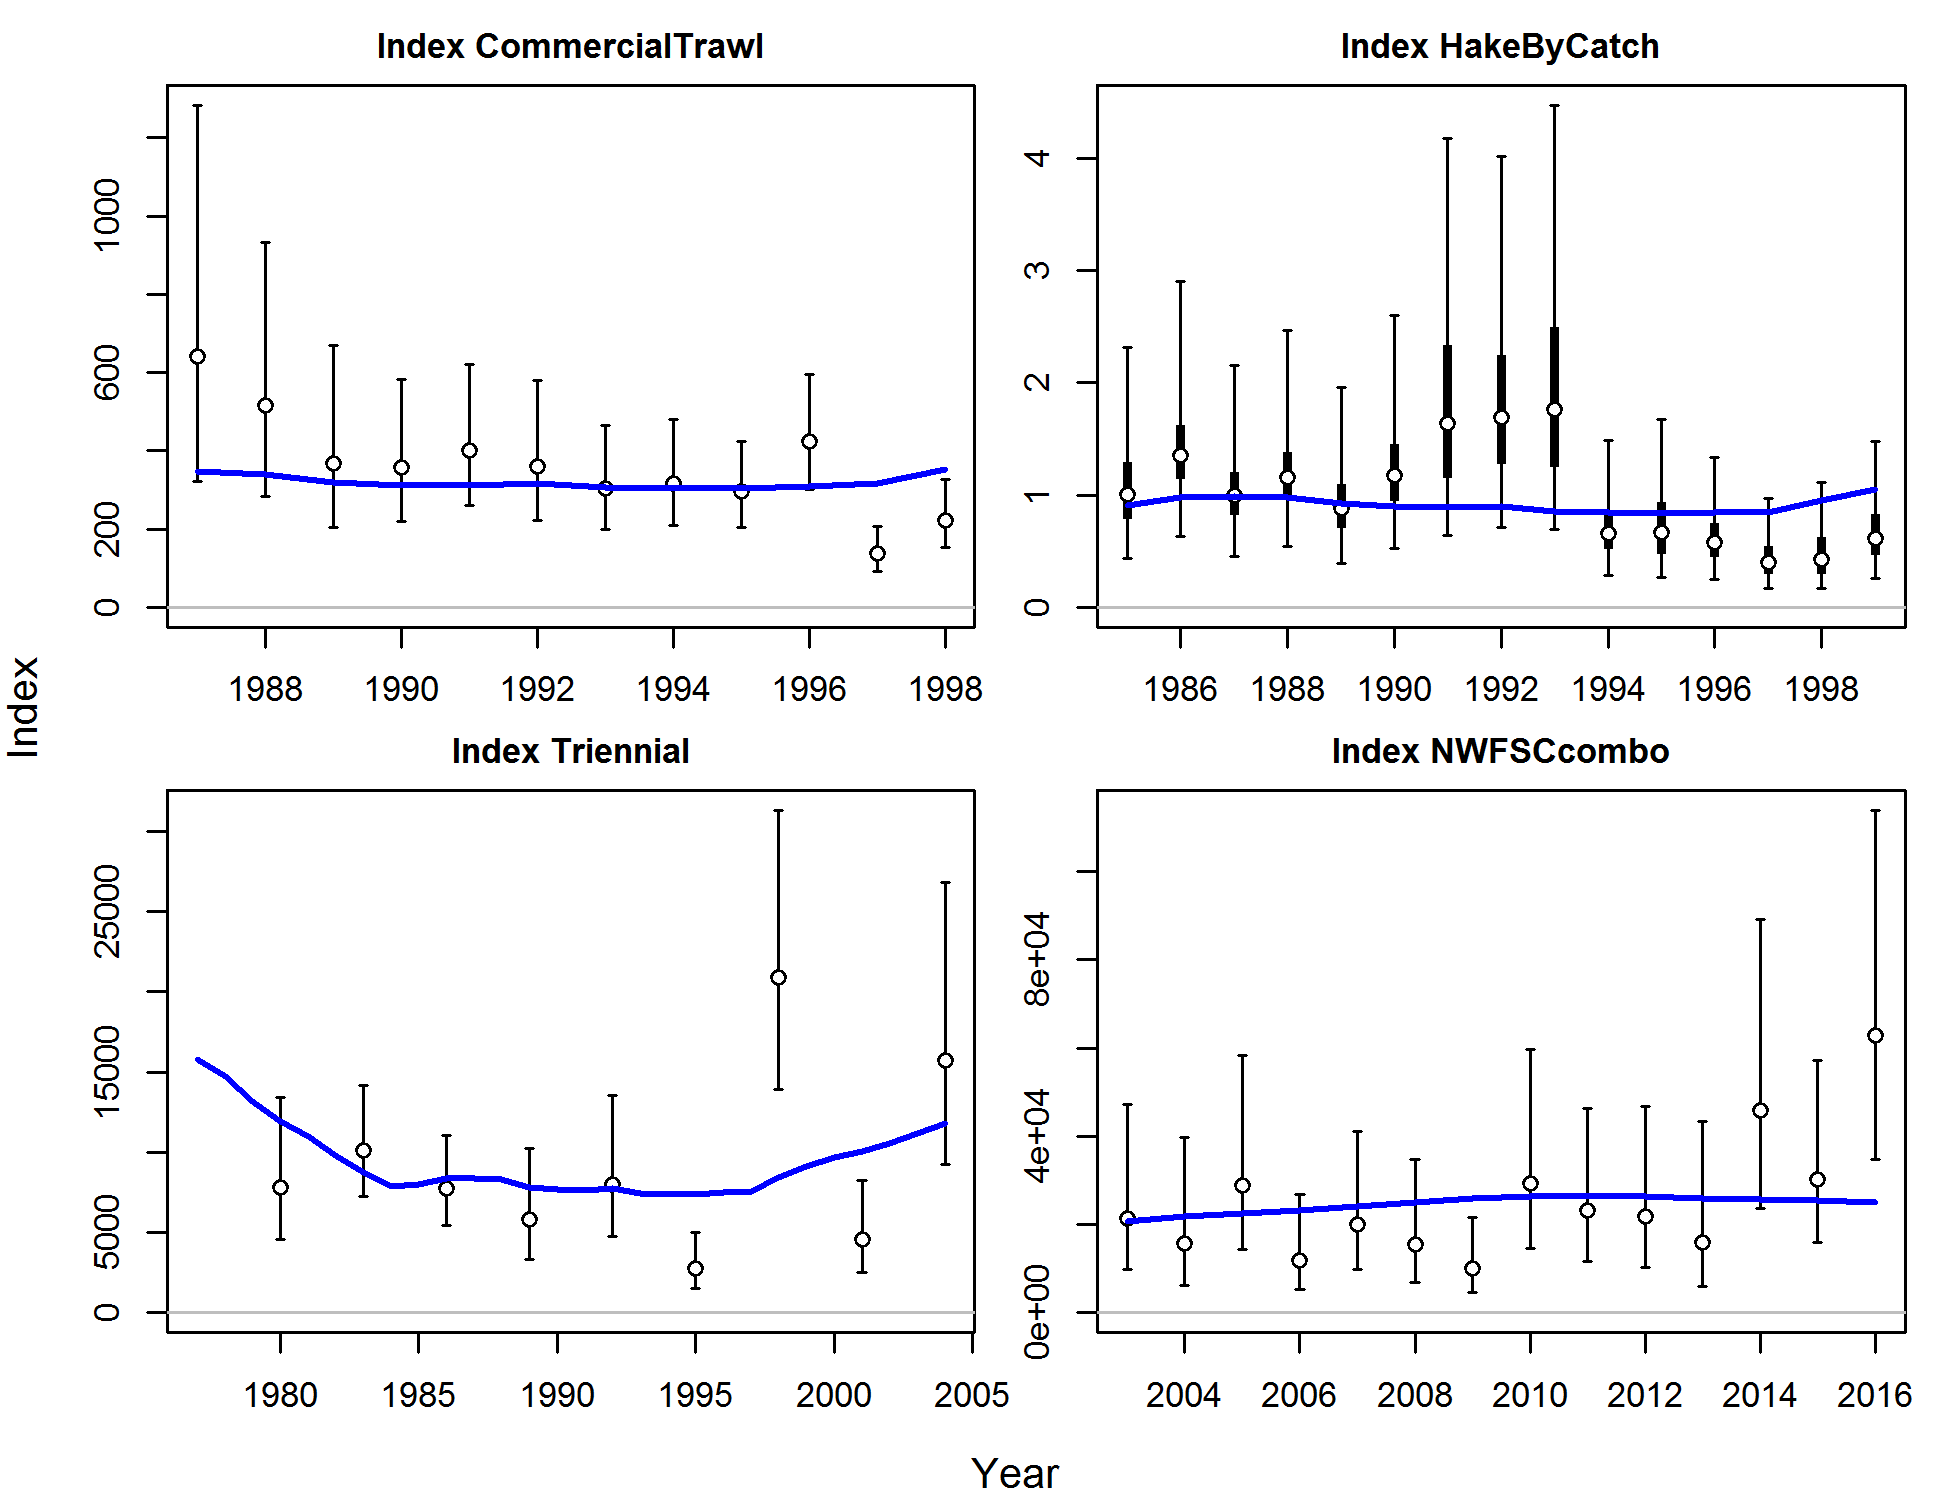
\includegraphics{r4ss/plots_mod1/index0_all_indices_fit.png}
\caption{Estimated fits to the CPUE and survey indices for the Northern
model. \label{fig:index_fits1}}
\end{figure}

\begin{figure}[htbp]
\centering
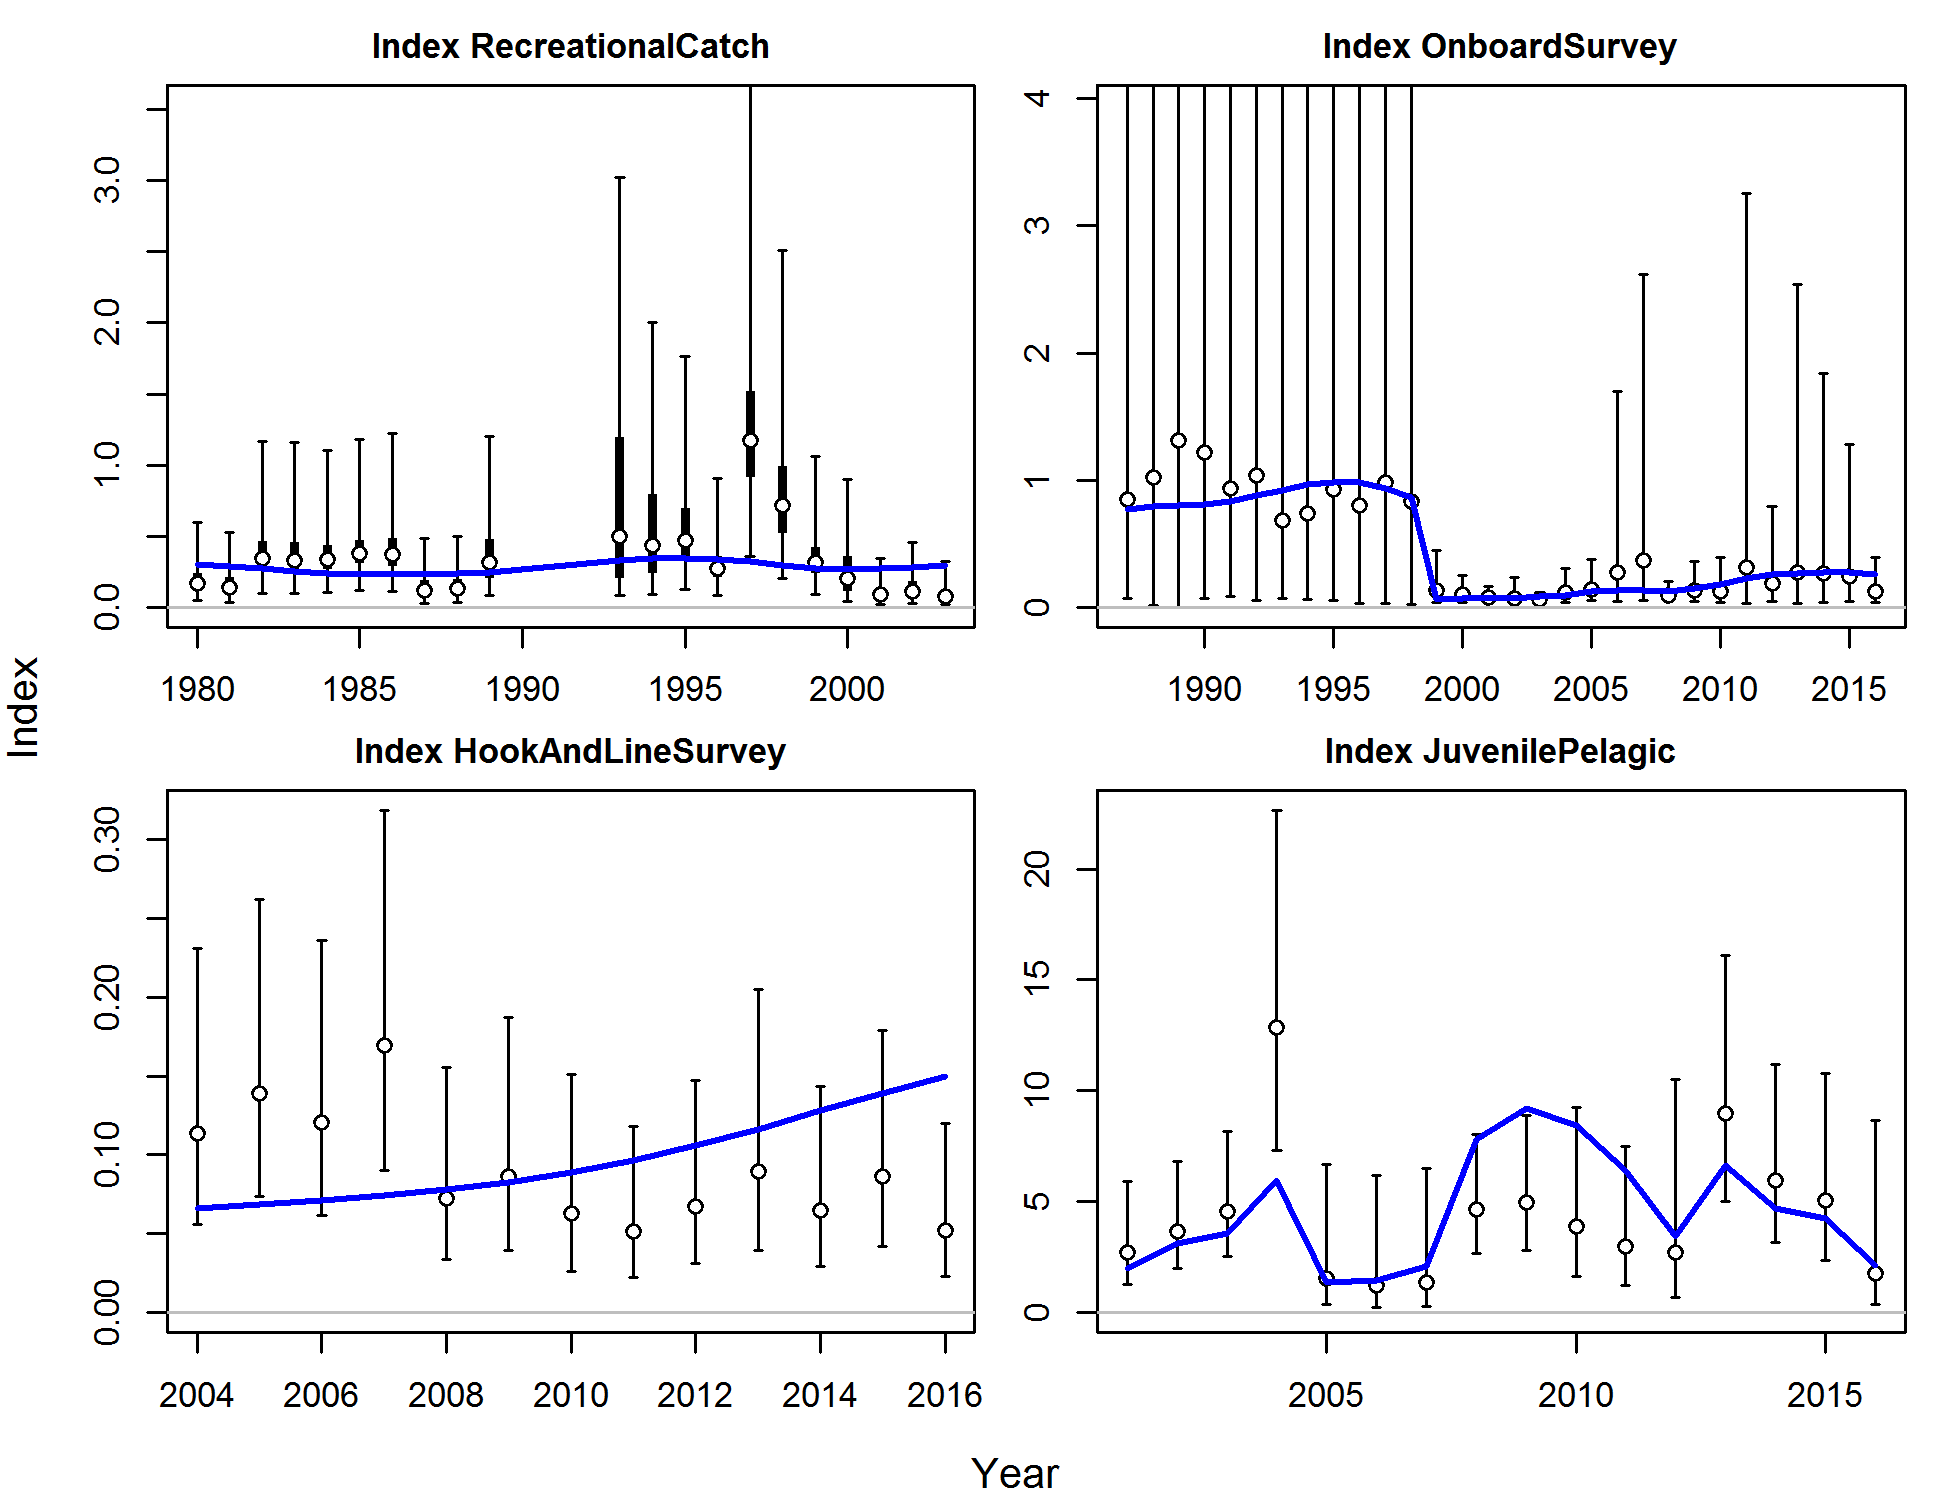
\includegraphics{r4ss/plots_mod2/index0_all_indices_fit.png}
\caption{Estimated fits to the CPUE and survey indices for the Southern
model. \label{fig:index_fits2}}
\end{figure}

\FloatBarrier 

\subsubsection{Fits to length compositions for Northern
model}\label{fits-to-length-compositions-for-northern-model}

\begin{figure}[htbp]
\centering
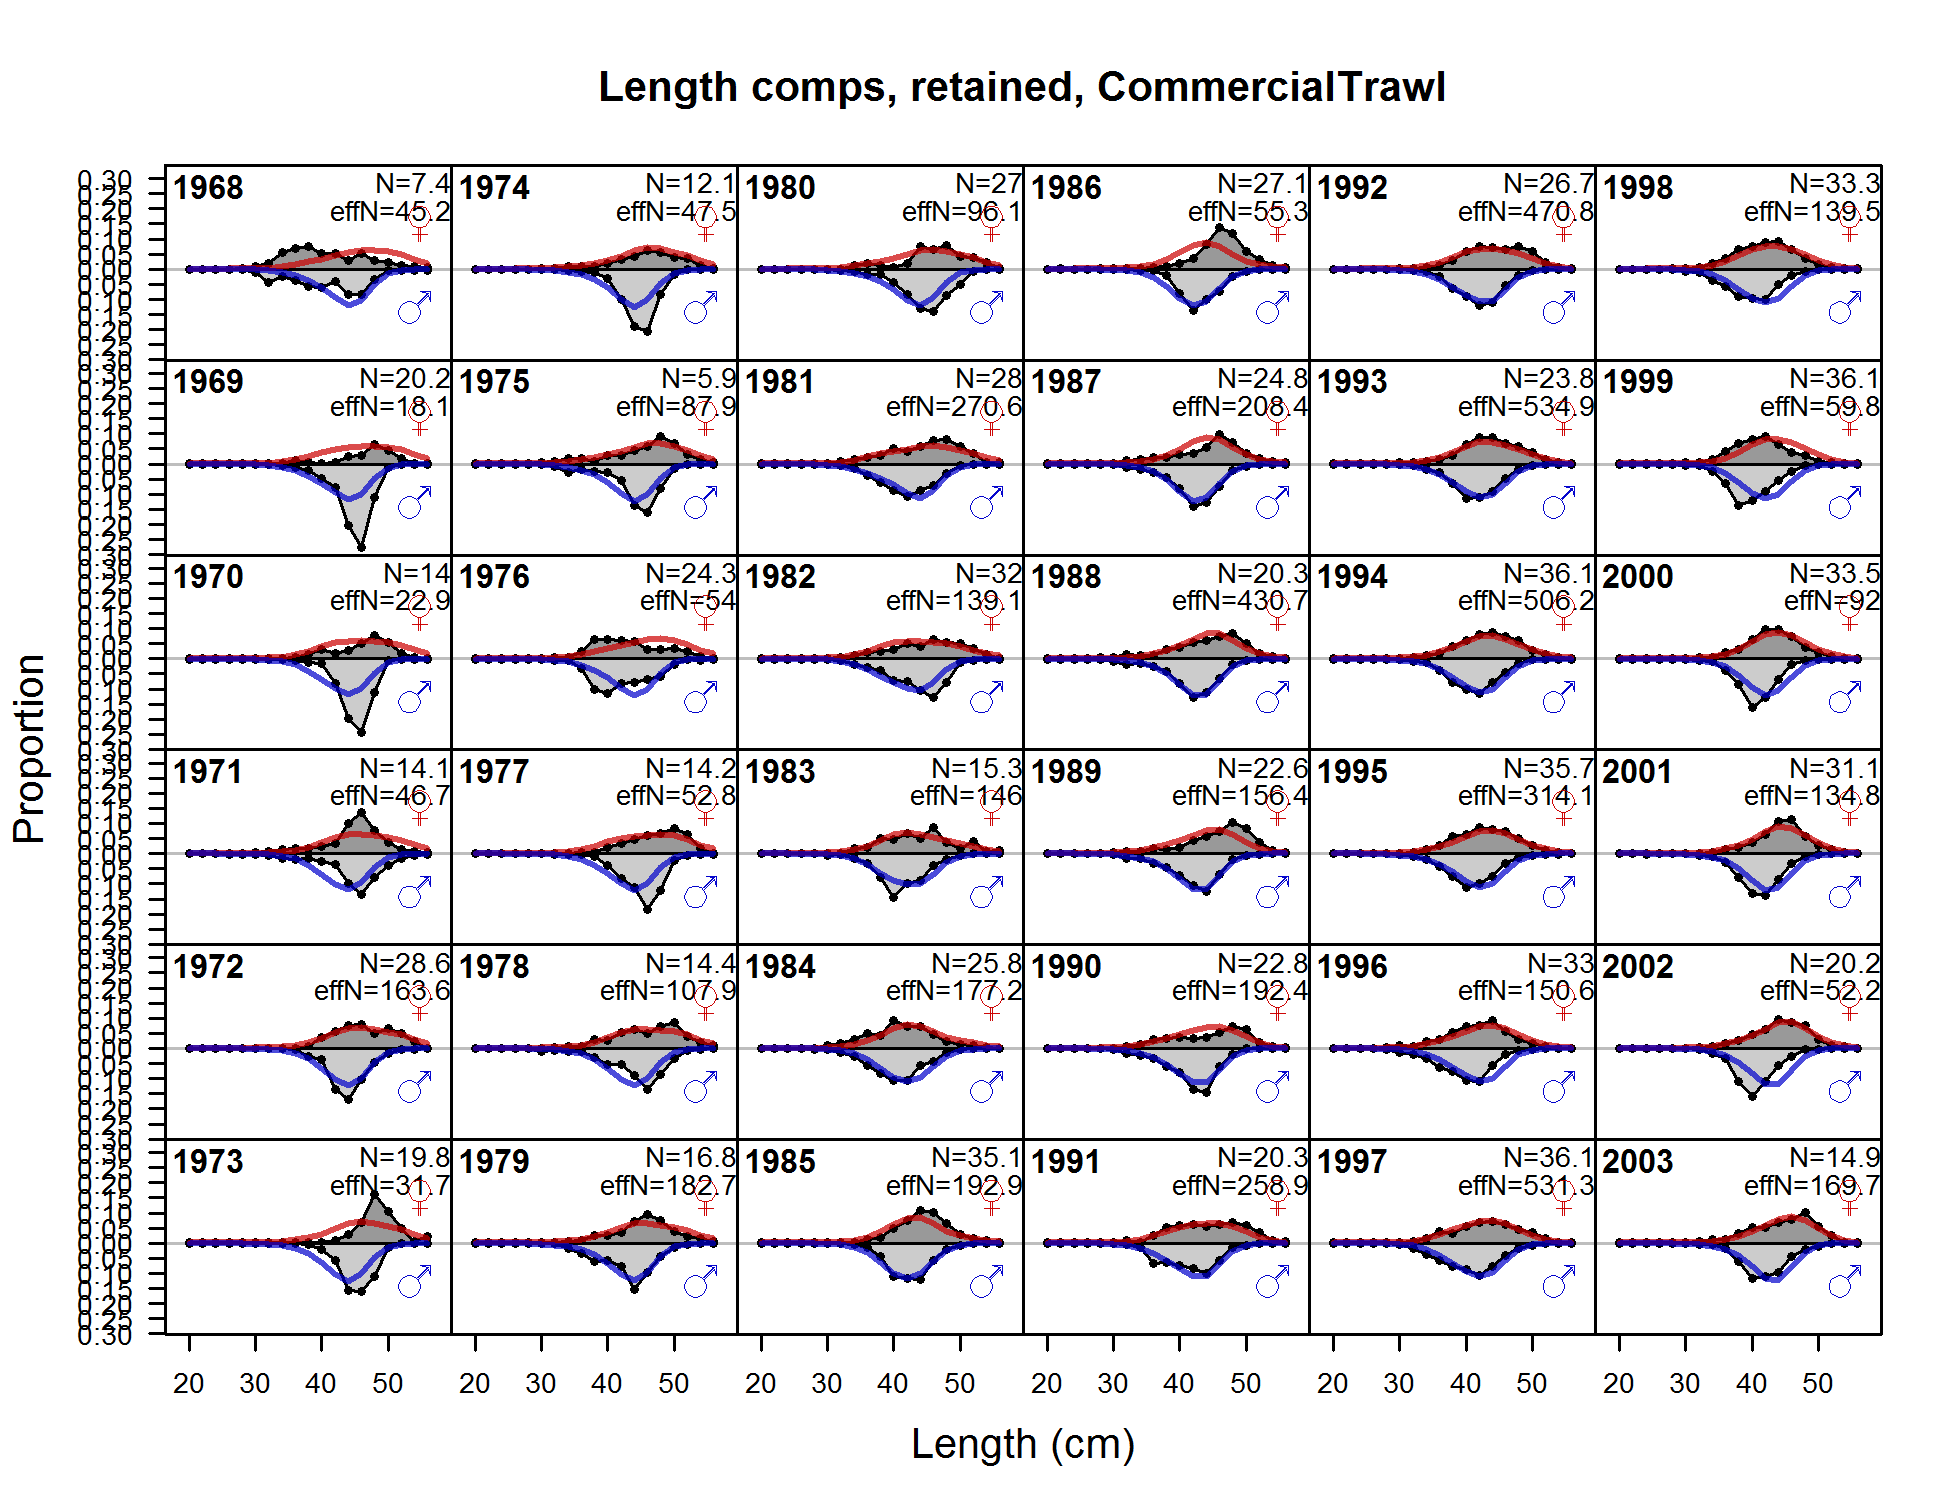
\includegraphics{./r4ss/plots_mod1/comp_lenfit_flt1mkt2_page1.png}
\caption{\textbf{Northern model} Length comps, retained, CommercialTrawl
(plot 1 of 2) \label{fig:mod1_1_comp_lenfit_flt1mkt2_page1}}
\end{figure}

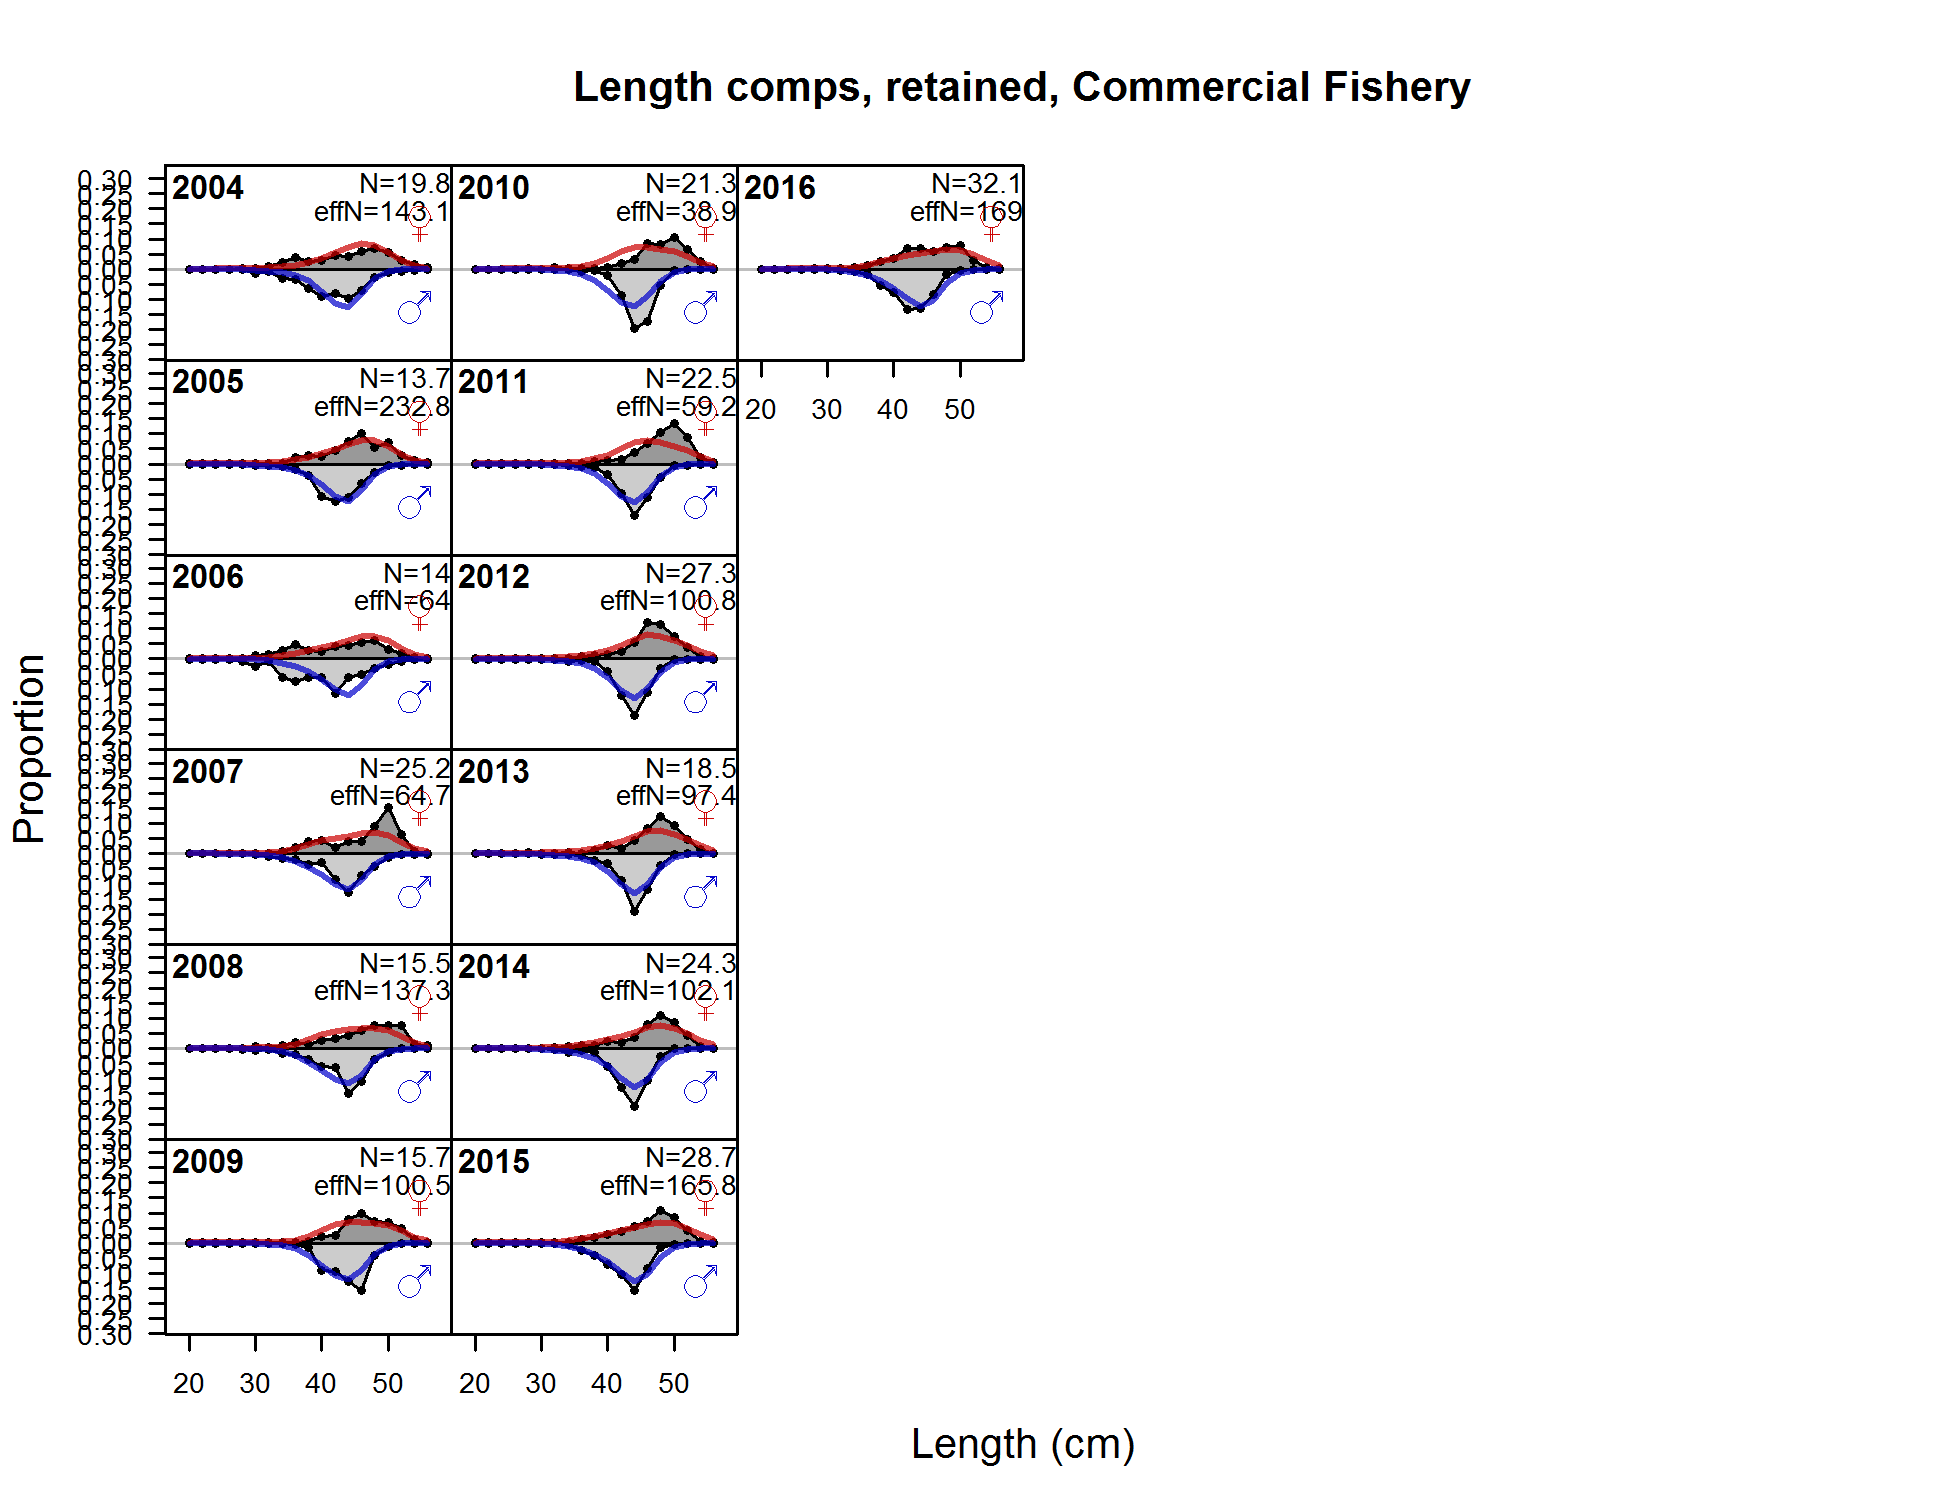
\includegraphics{./r4ss/plots_mod1/comp_lenfit_flt1mkt2_page2.png}

\begin{center} 

            Figure continued from previous page 

            \end{center}

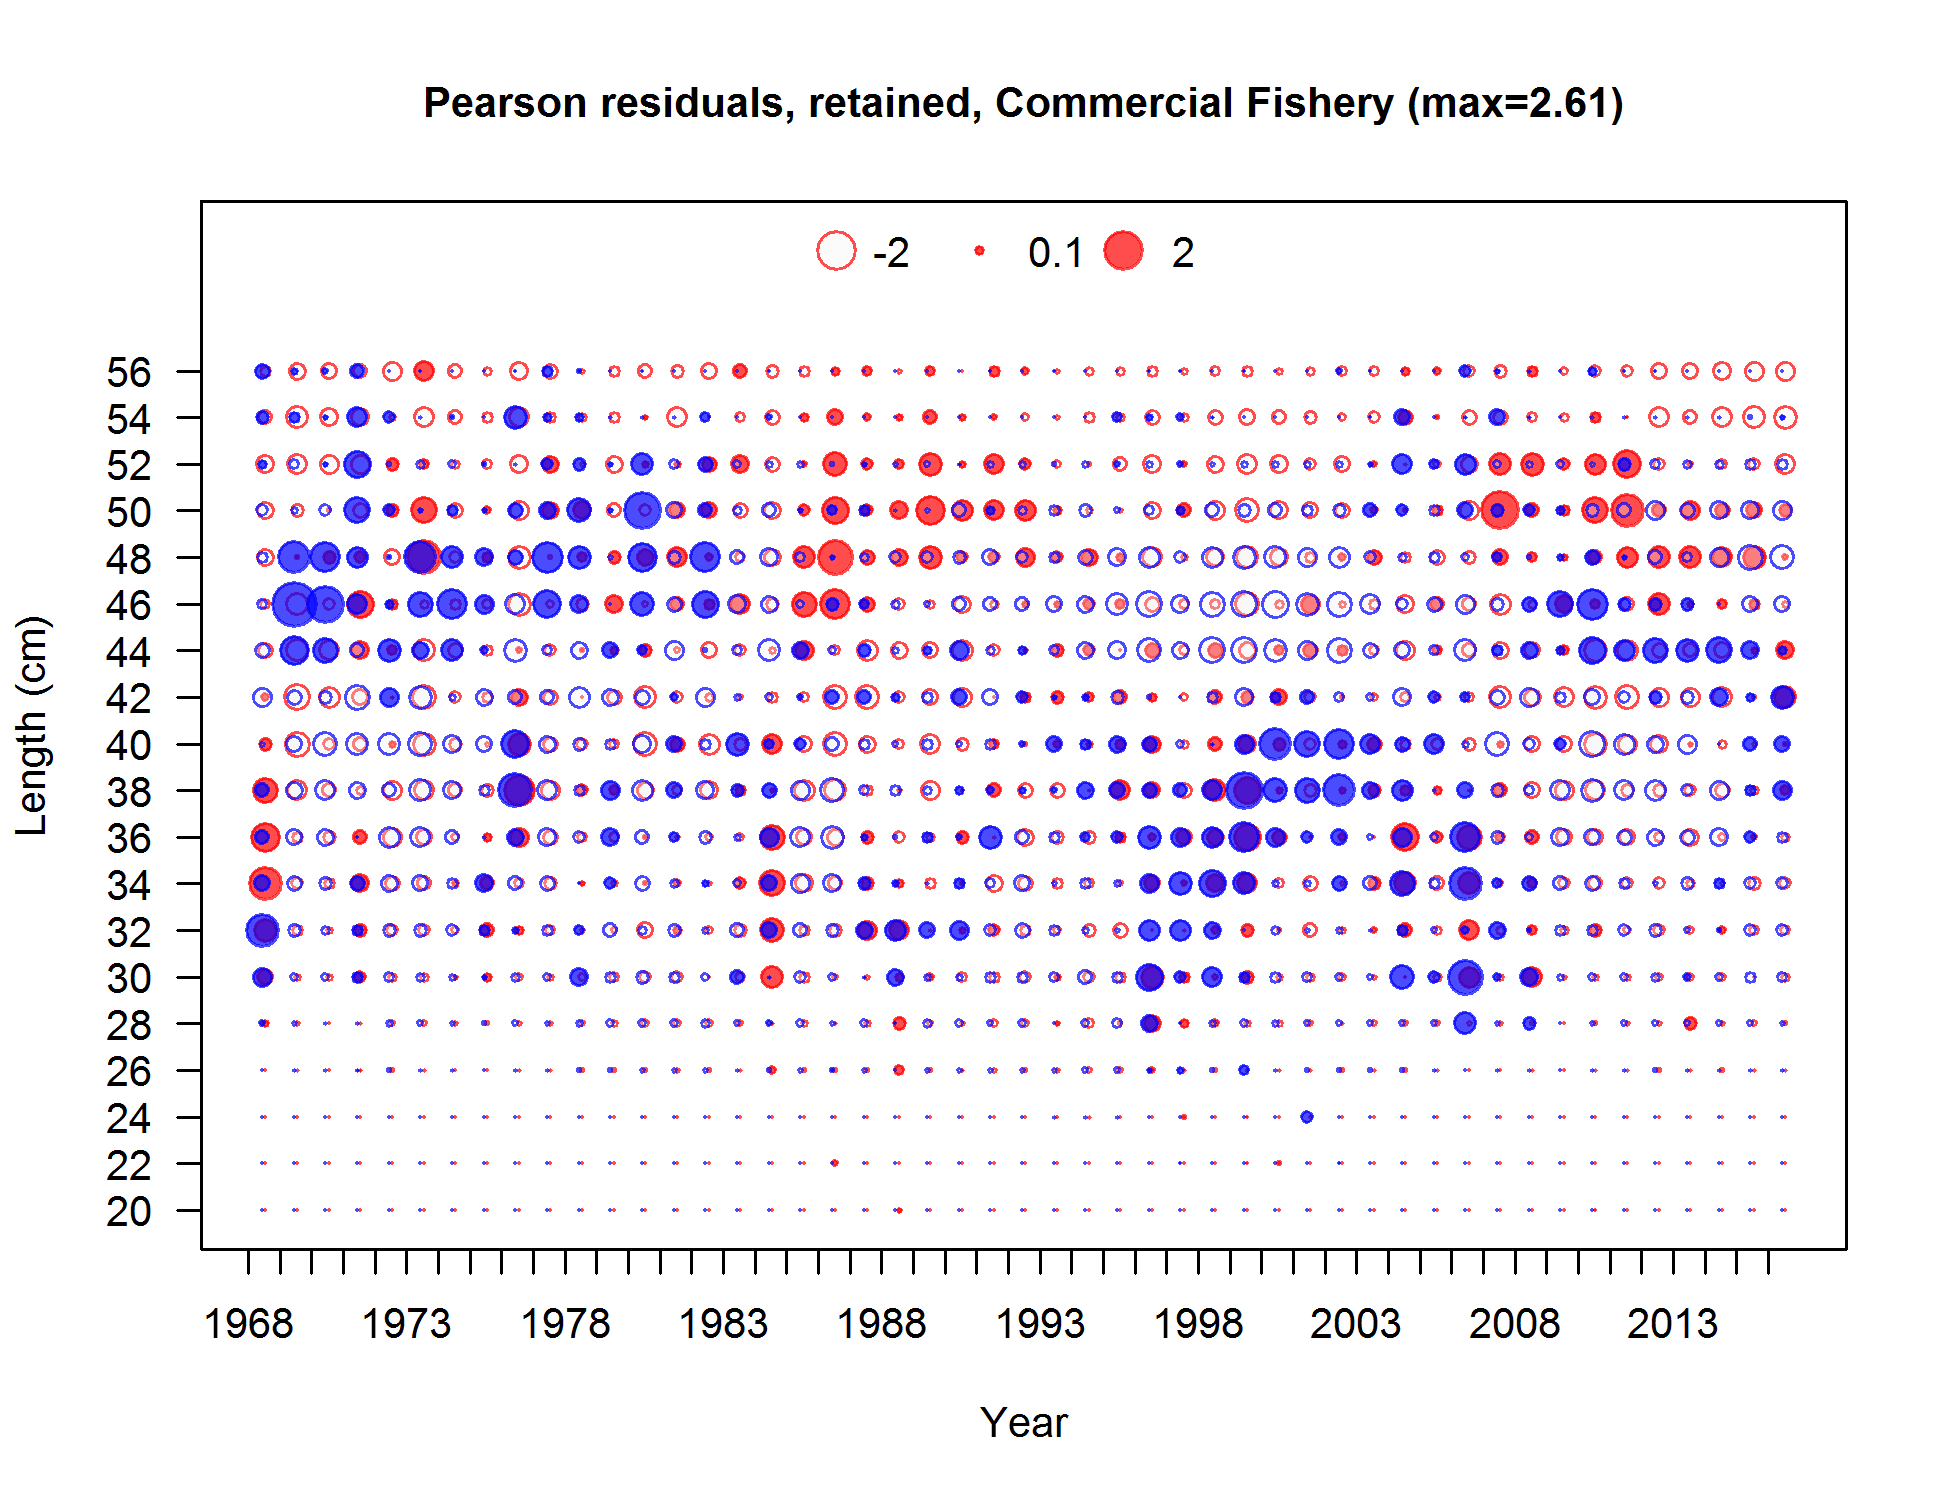
\includegraphics{./r4ss/plots_mod1/comp_lenfit_residsflt1mkt2_page2.png}

\begin{center} 

            Figure continued from previous page 

            \end{center}

\begin{figure}[htbp]
\centering
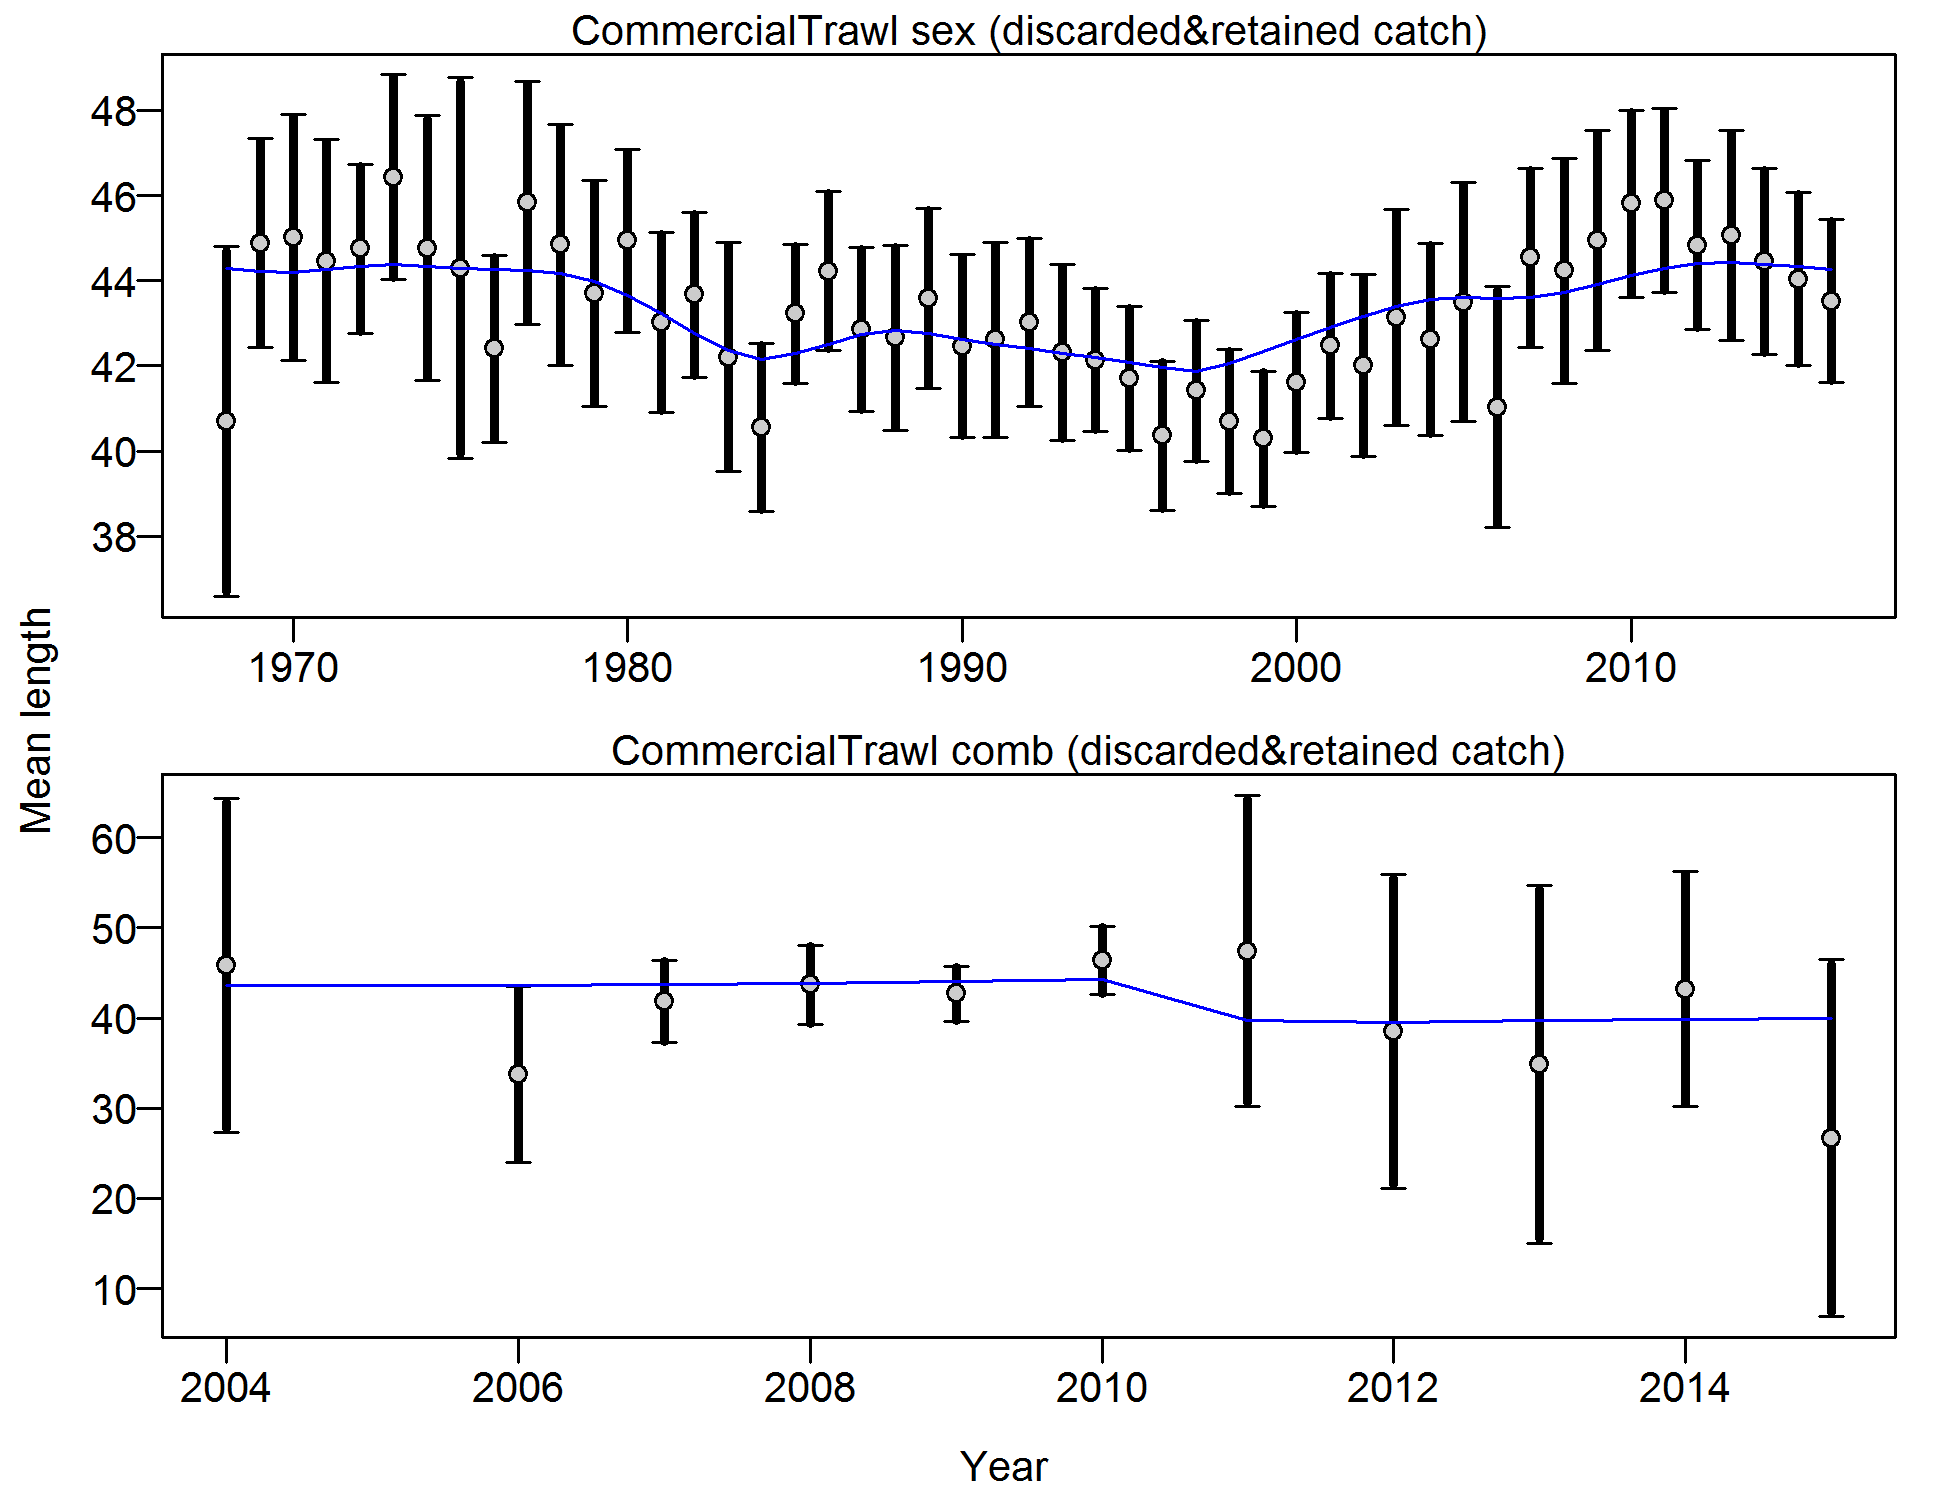
\includegraphics{./r4ss/plots_mod1/comp_lenfit_data_weighting_TA1.8_CommercialTrawl.png}
\caption{\textbf{Northern model} Francis data weighting method TA1.8:
CommercialTrawl Suggested sample size adjustment (with 95\% interval)
for len data from CommercialTrawl: 0.9488 (0.7164\_1.4056) For more
info, see Francis, R.I.C.C. (2011). Data weighting in statistical
fisheries stock assessment models. Can. J. Fish. Aquat. Sci. 68:
1124\_1138.
\label{fig:mod1_5_comp_lenfit_data_weighting_TA1.8_CommercialTrawl}}
\end{figure}

\begin{figure}[htbp]
\centering
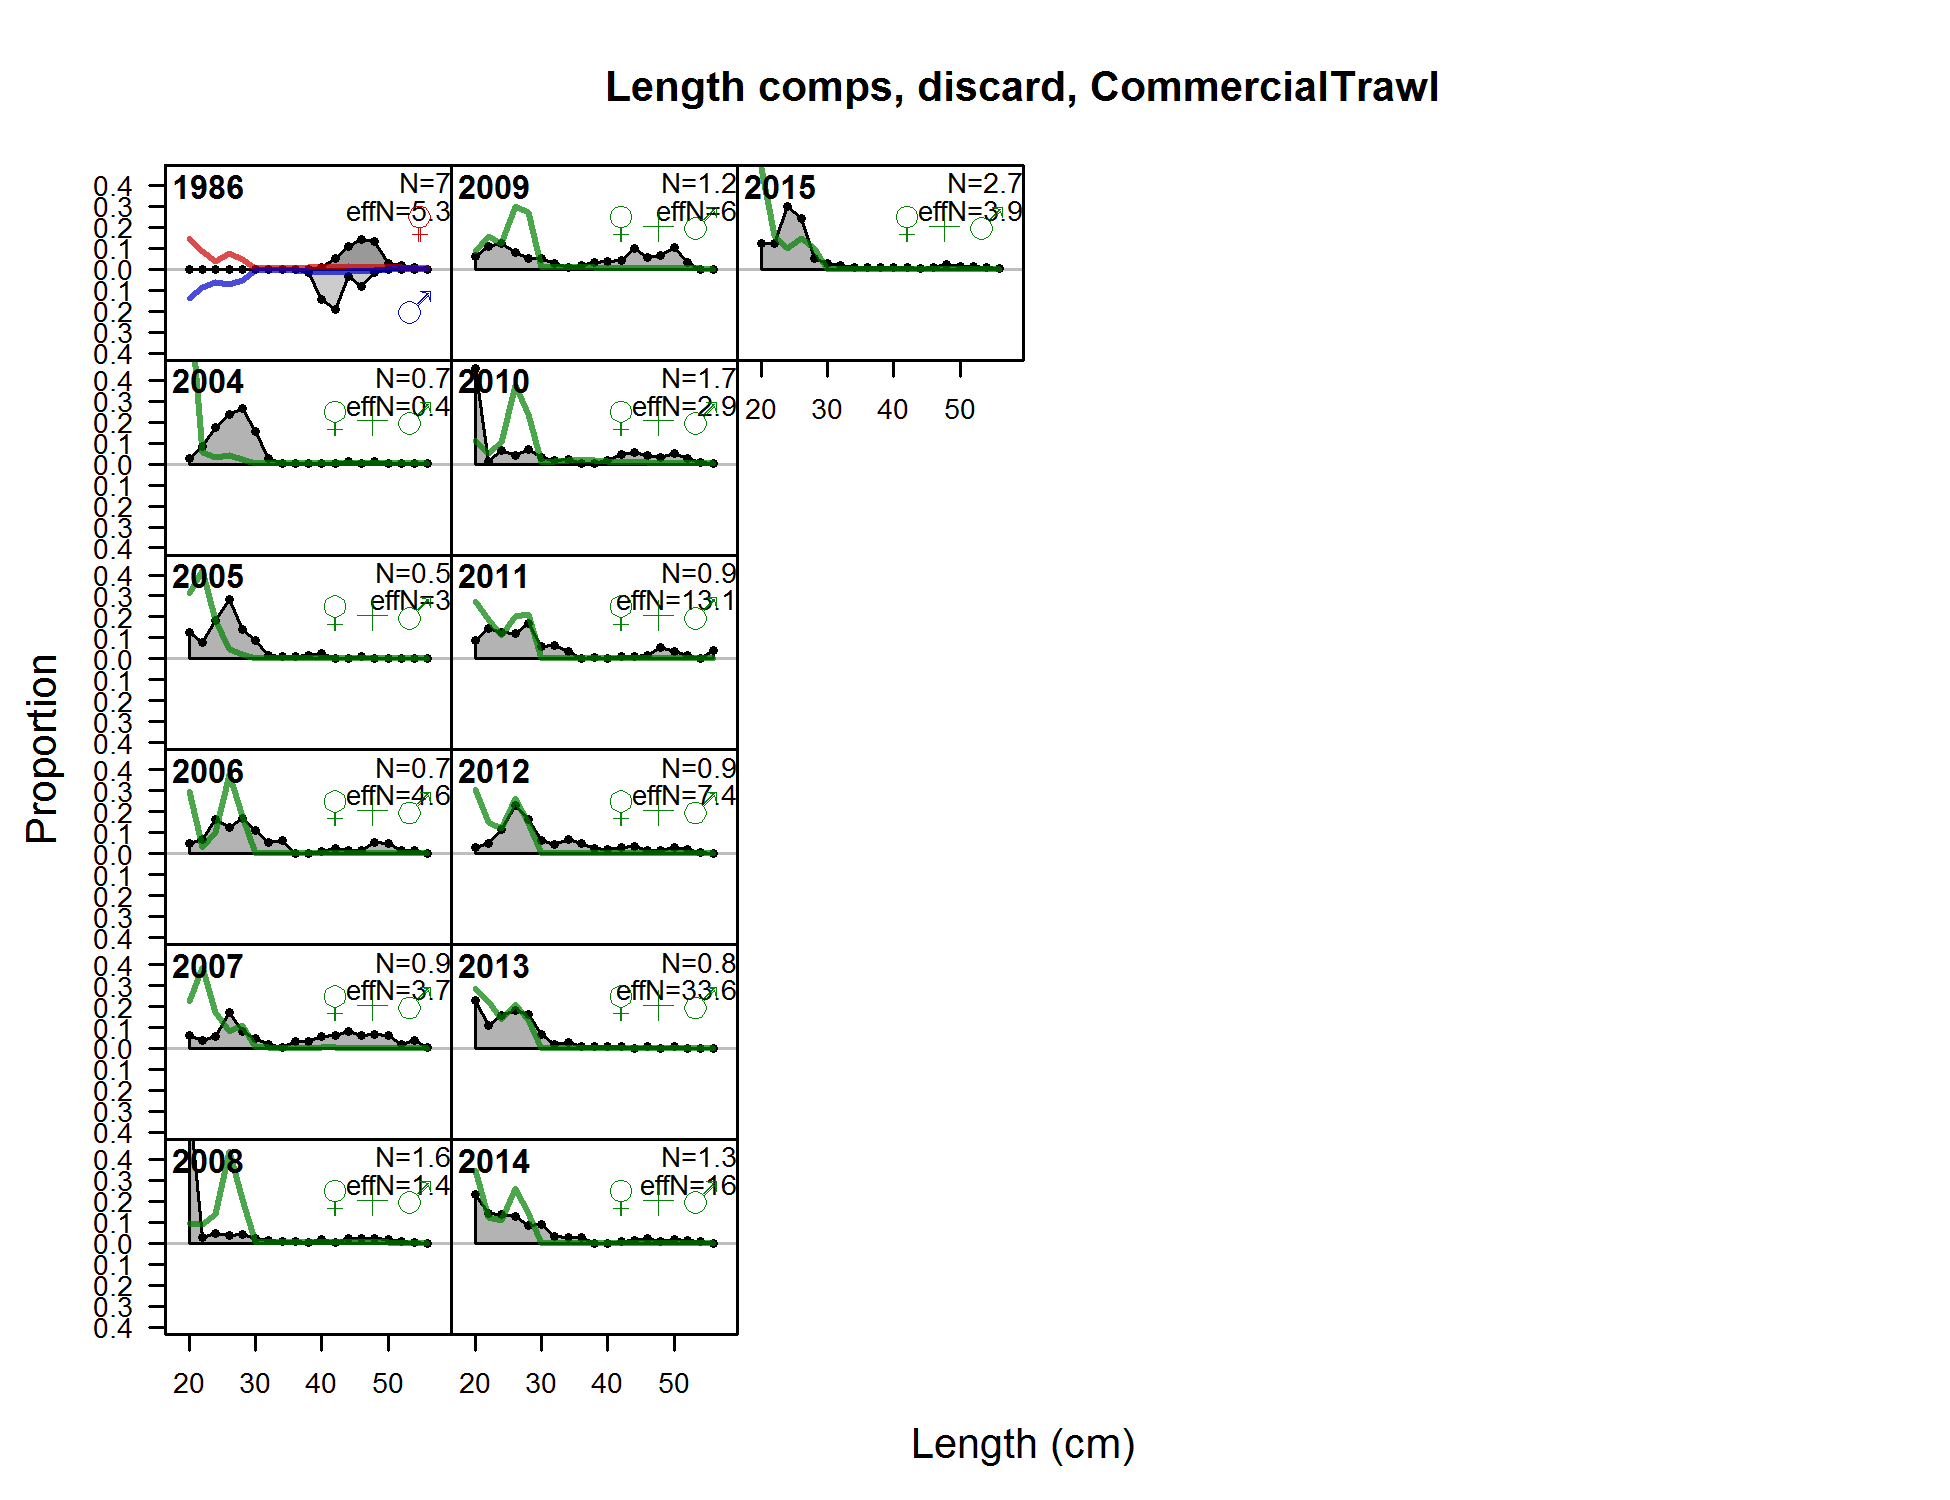
\includegraphics{./r4ss/plots_mod1/comp_lenfit_flt1mkt1.png}
\caption{\textbf{Northern model} Length comps, discard, CommercialTrawl
\label{fig:mod1_6_comp_lenfit_flt1mkt1}}
\end{figure}

\begin{figure}[htbp]
\centering
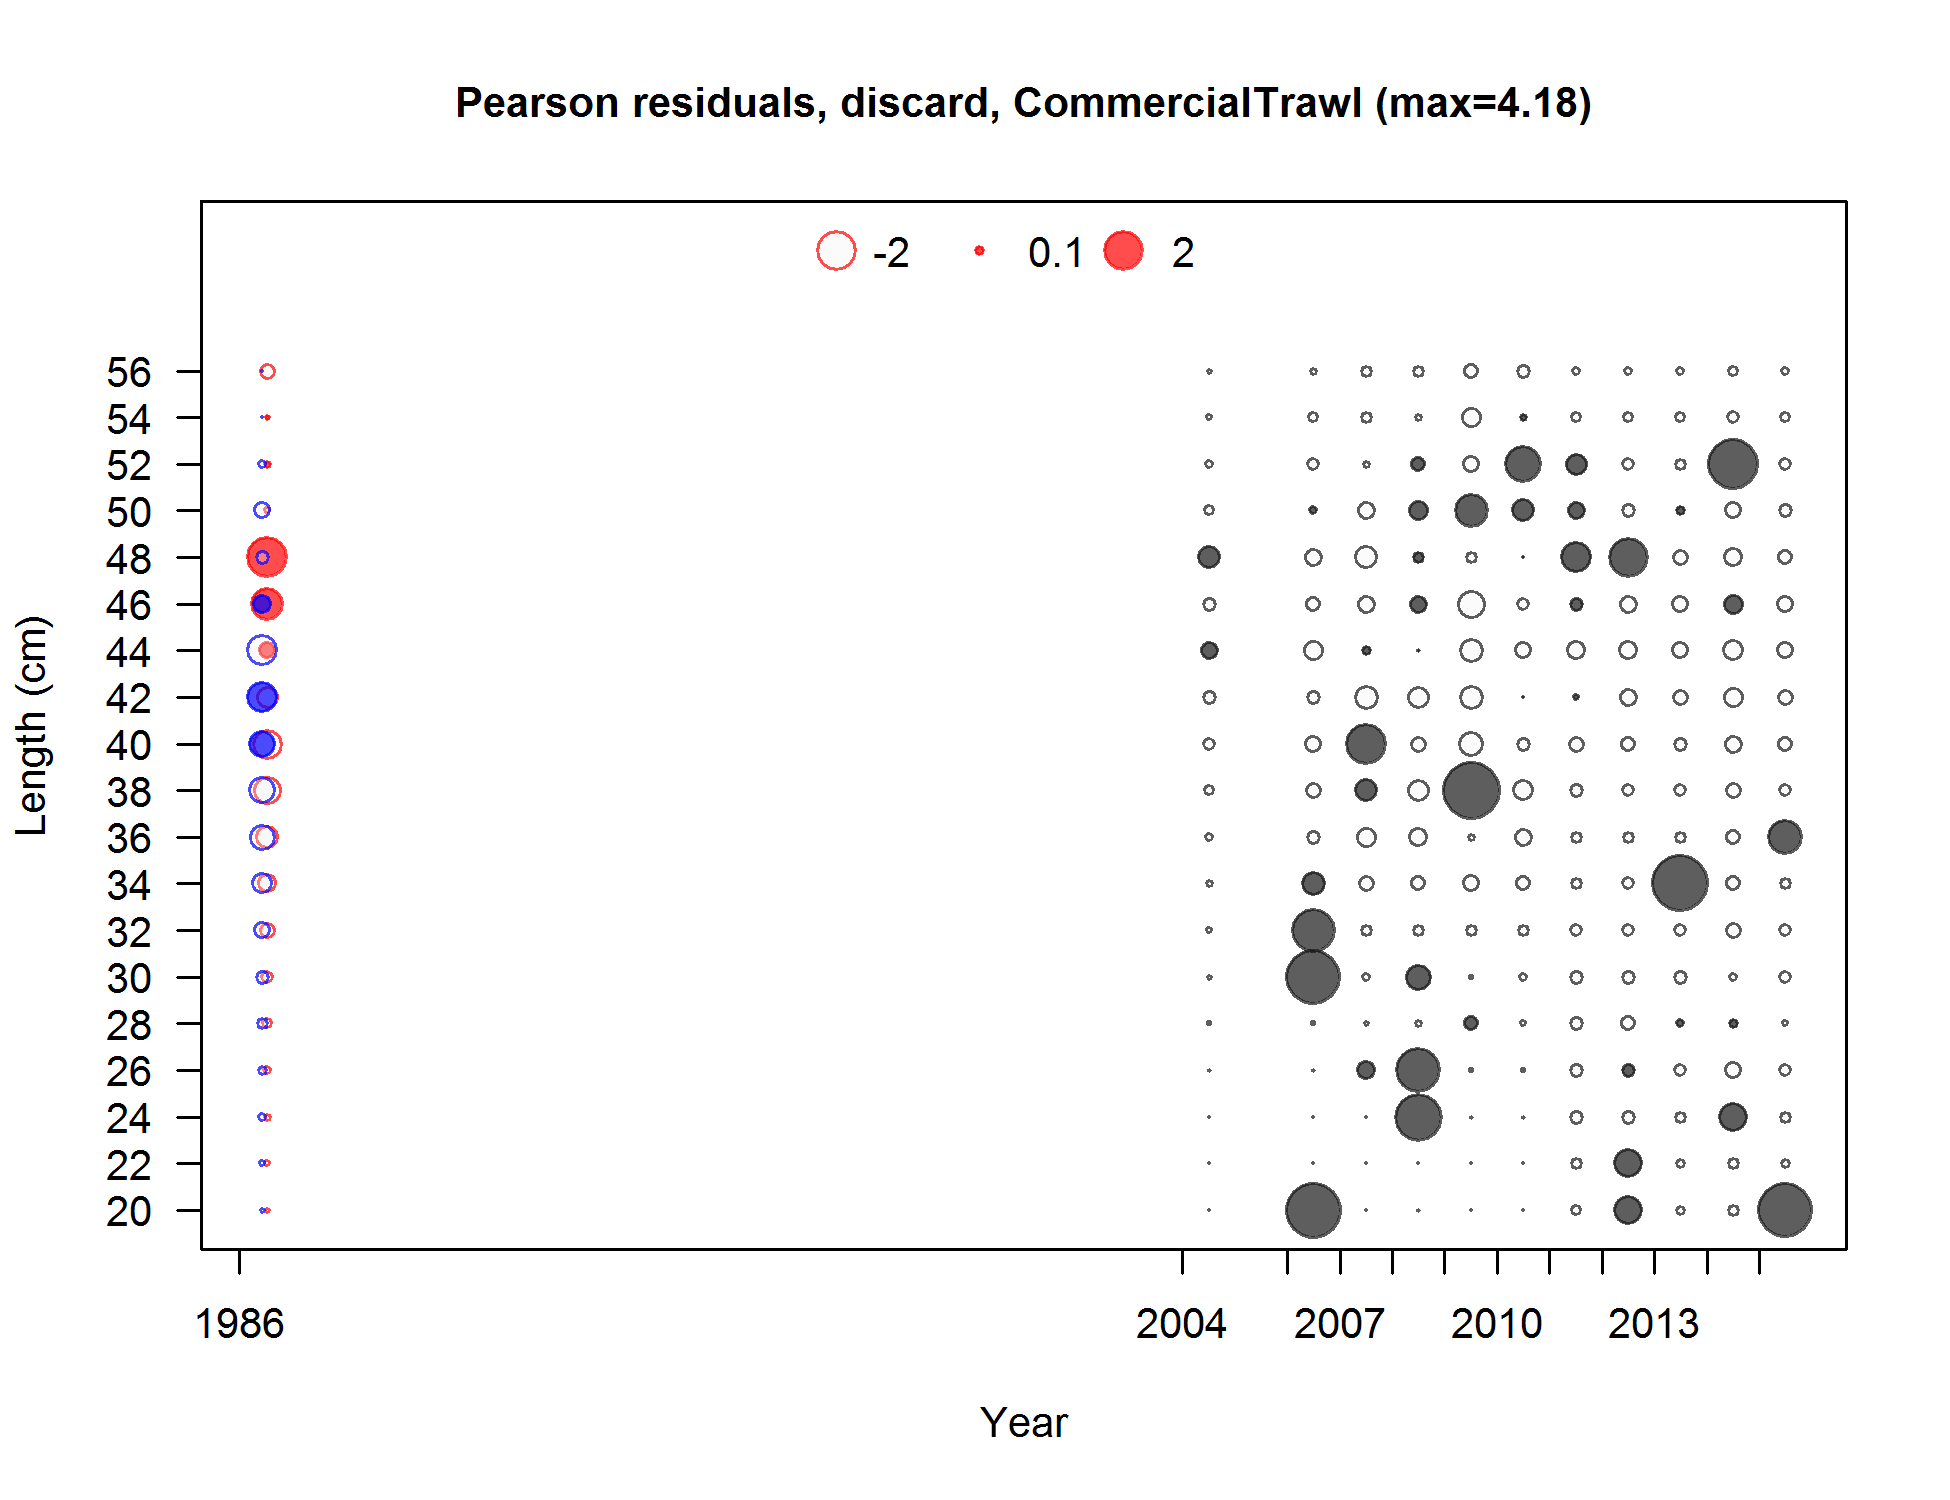
\includegraphics{./r4ss/plots_mod1/comp_lenfit_residsflt1mkt1.png}
\caption{\textbf{Northern model} Pearson residuals, discard,
CommercialTrawl (max=4.18)\\
Closed bubbles are positive residuals (observed \textgreater{} expected)
and open bubbles are negative residuals (observed \textless{} expected).
\label{fig:mod1_7_comp_lenfit_residsflt1mkt1}}
\end{figure}

\begin{figure}[htbp]
\centering
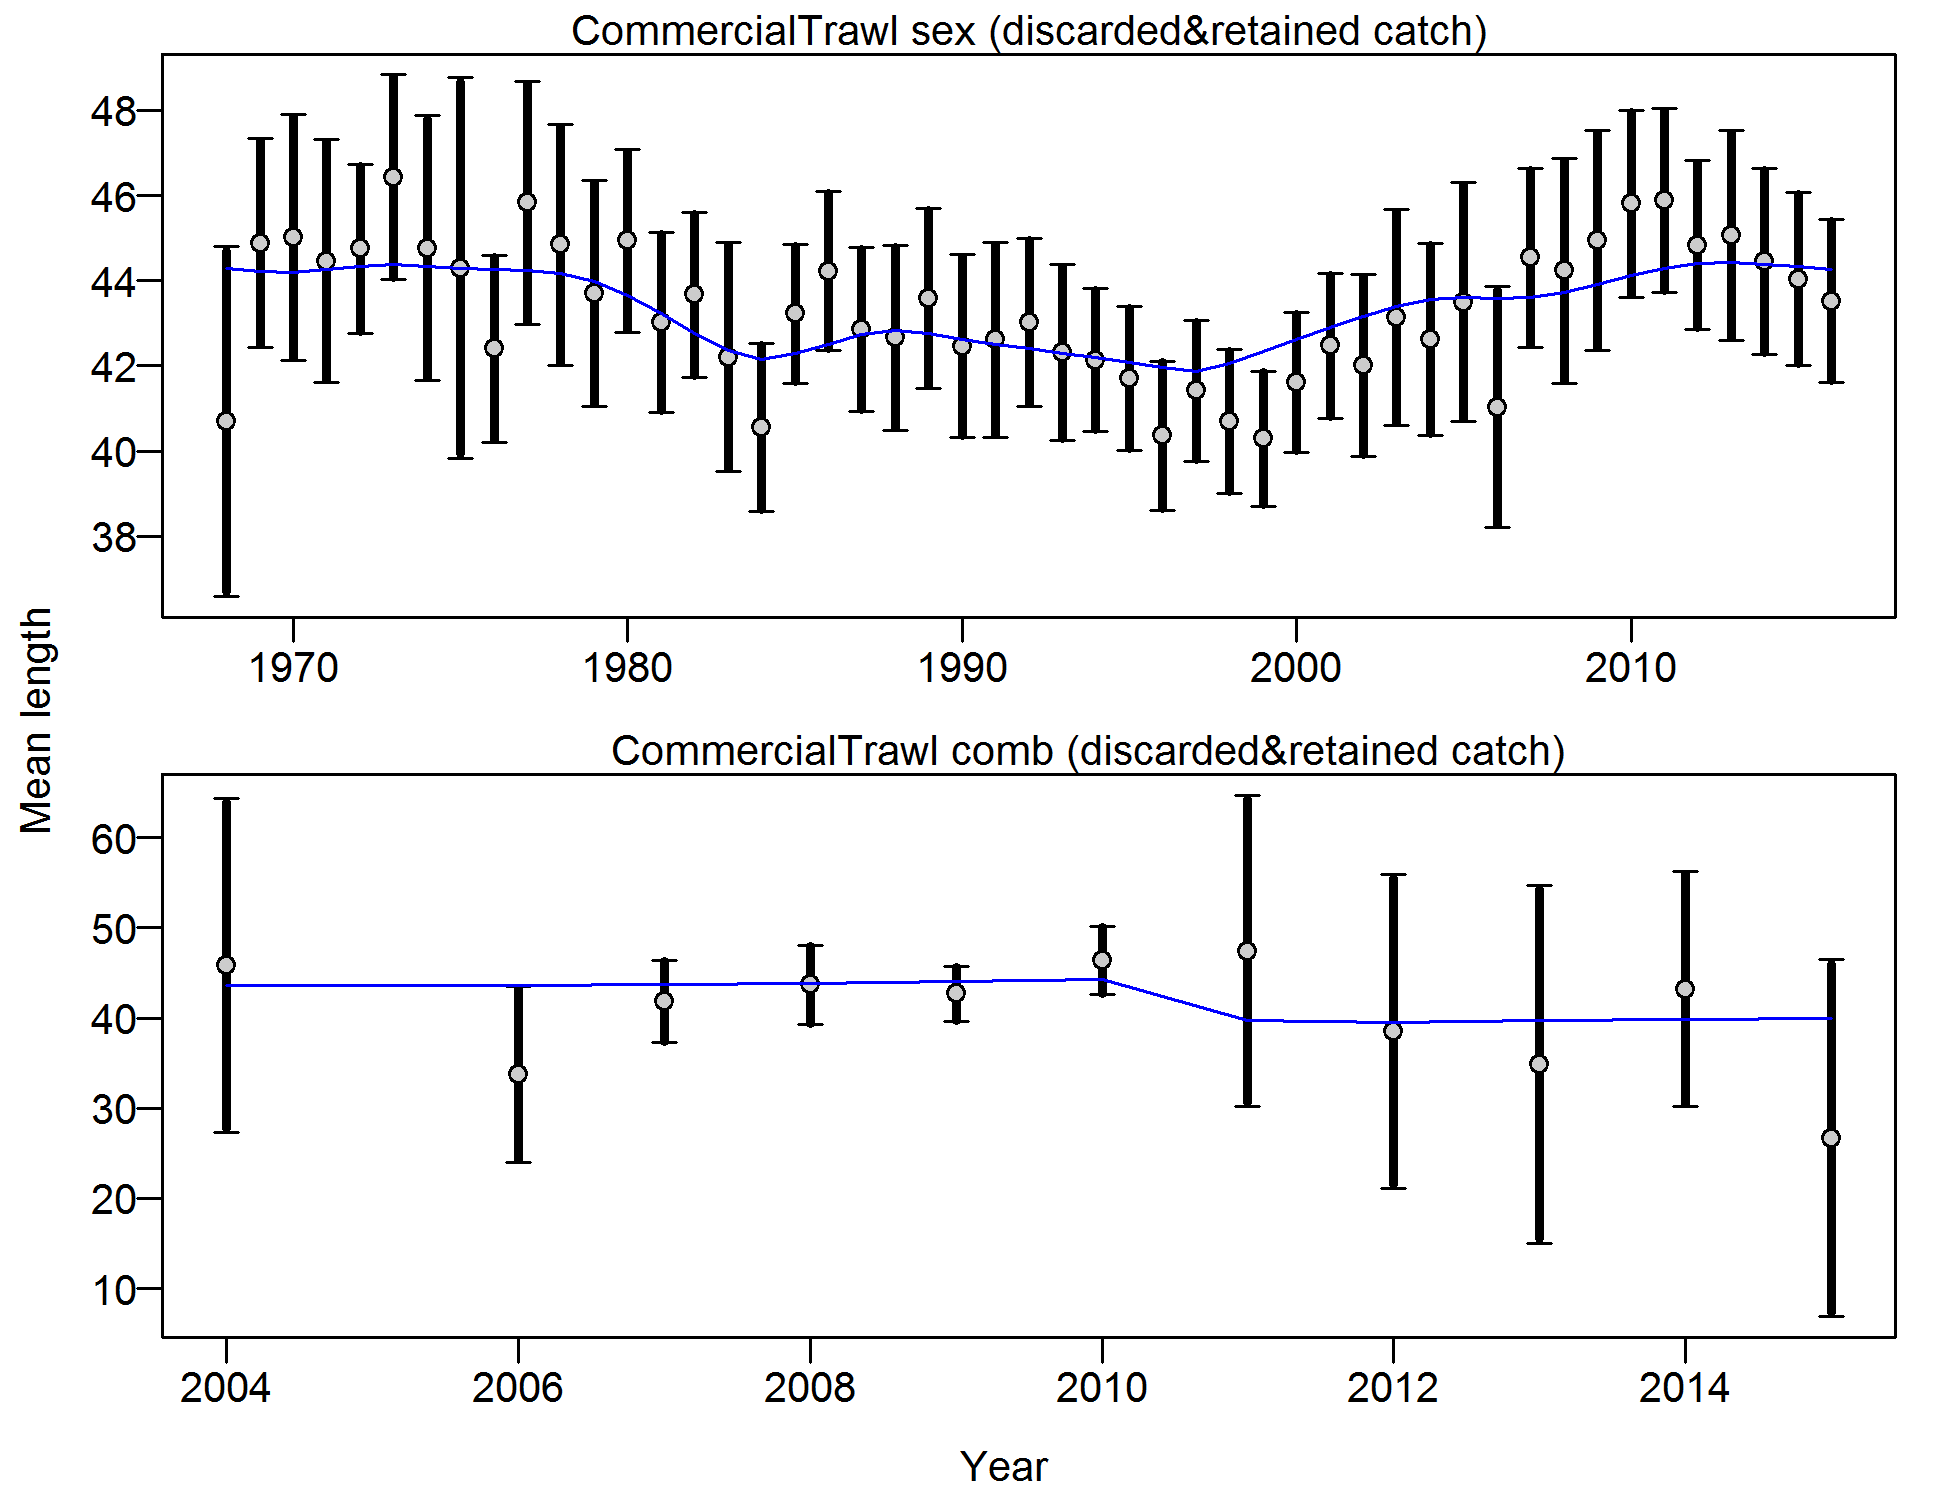
\includegraphics{./r4ss/plots_mod1/comp_lenfit_data_weighting_TA1.8_CommercialTrawl.png}
\caption{\textbf{Northern model} Francis data weighting method TA1.8:
CommercialTrawl Suggested sample size adjustment (with 95\% interval)
for len data from CommercialTrawl: 0.9488 (0.7195\_1.4058) For more
info, see Francis, R.I.C.C. (2011). Data weighting in statistical
fisheries stock assessment models. Can. J. Fish. Aquat. Sci. 68:
1124\_1138.
\label{fig:mod1_9_comp_lenfit_data_weighting_TA1.8_CommercialTrawl}}
\end{figure}

\begin{figure}[htbp]
\centering
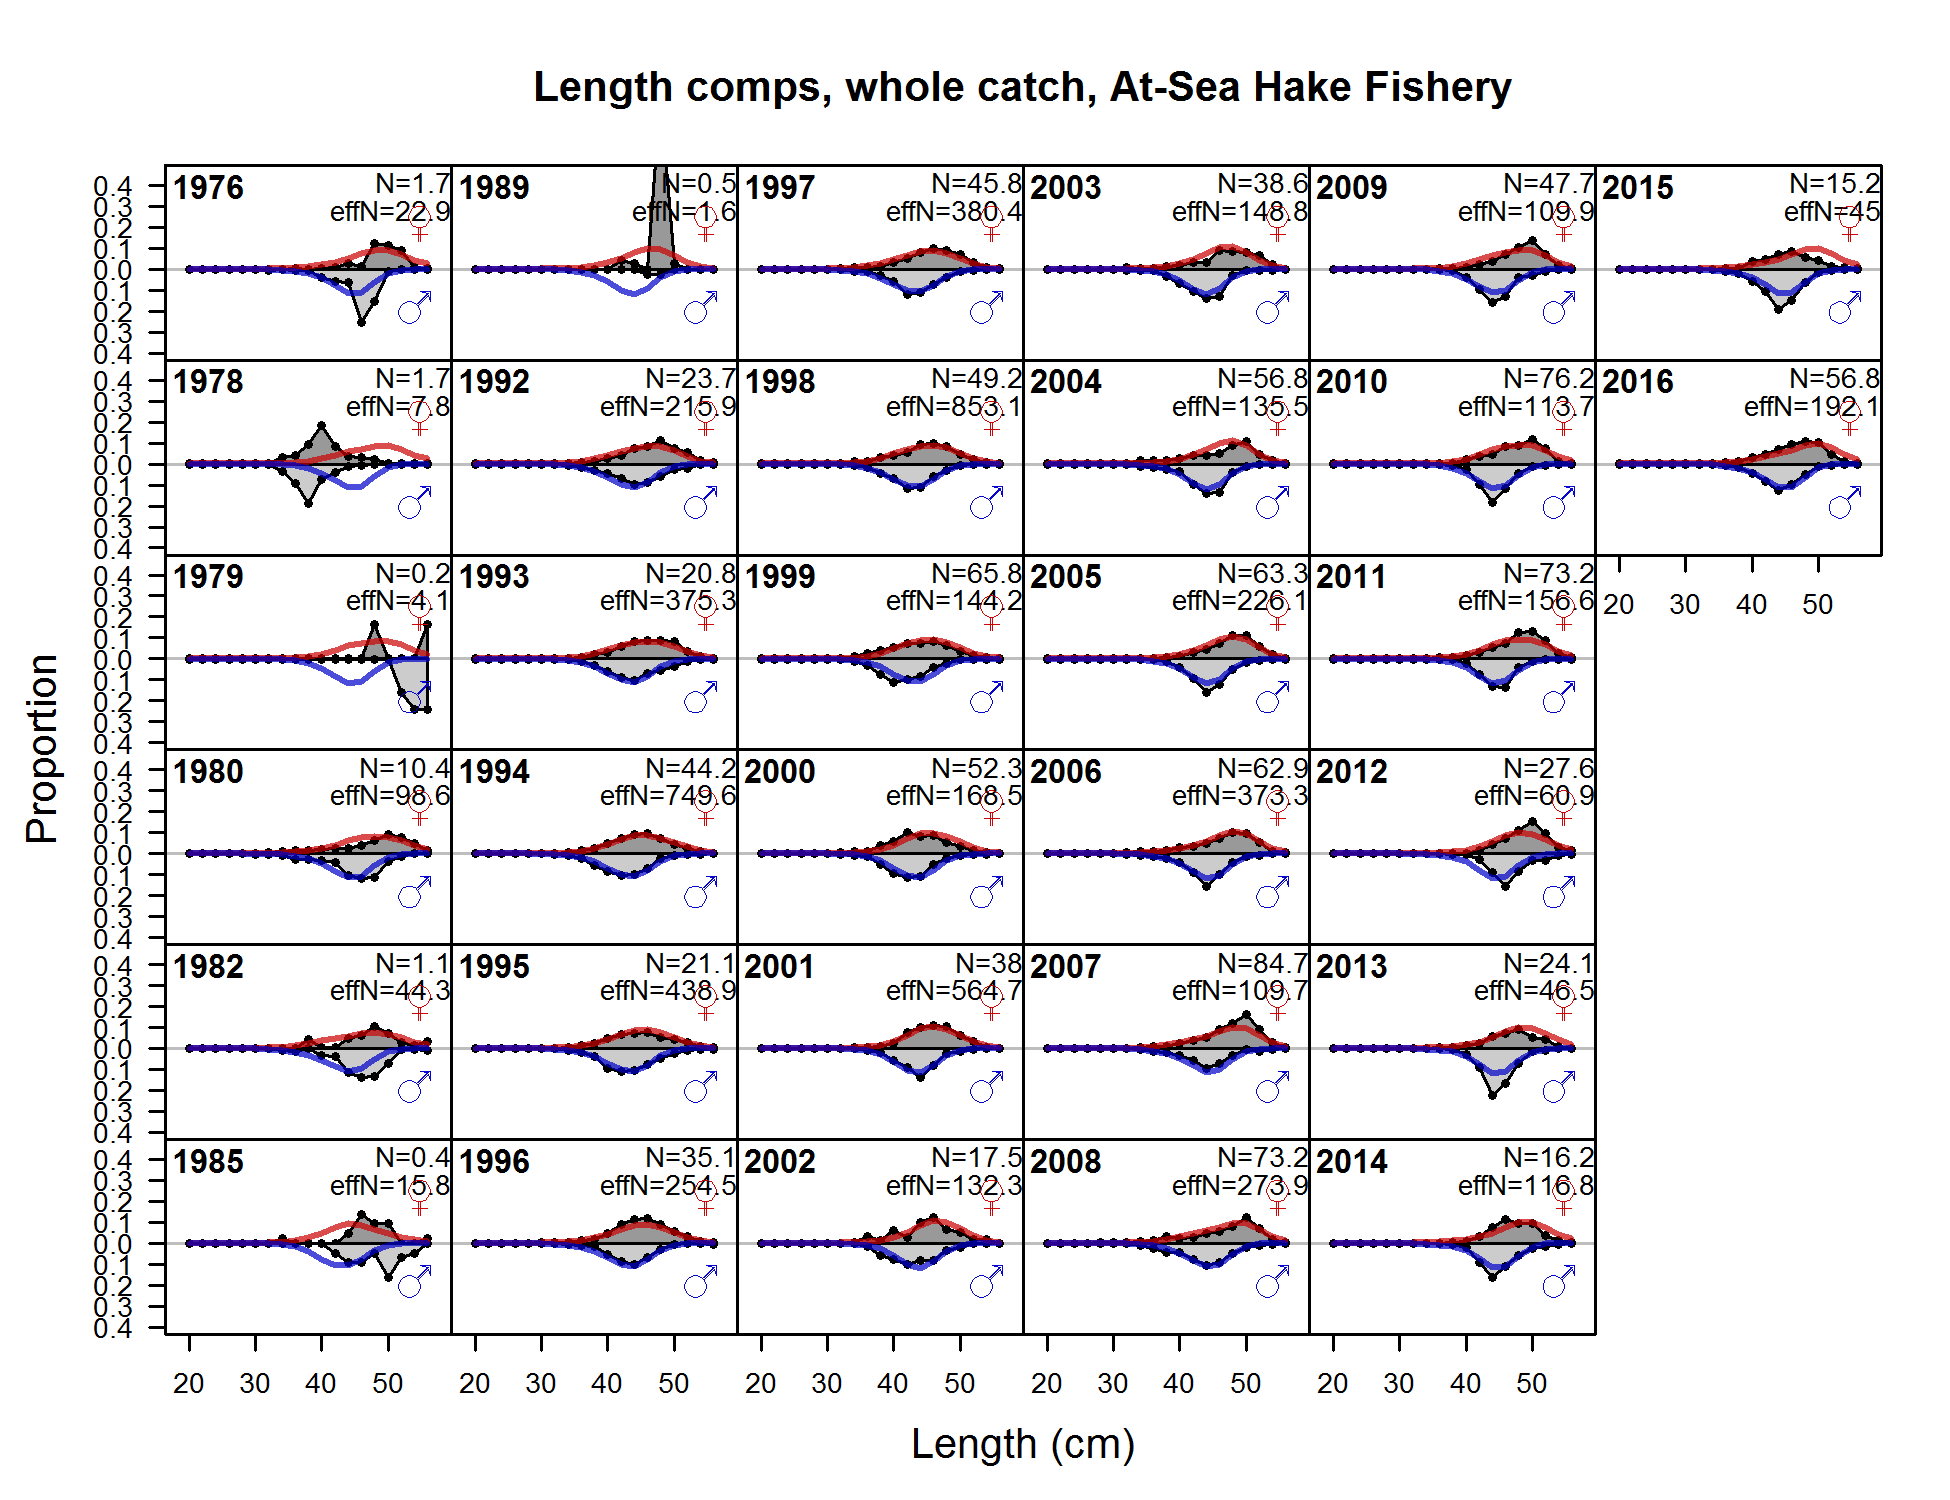
\includegraphics{./r4ss/plots_mod1/comp_lenfit_flt2mkt0.png}
\caption{\textbf{Northern model} Length comps, whole catch, HakeByCatch
\label{fig:mod1_10_comp_lenfit_flt2mkt0}}
\end{figure}

\begin{figure}[htbp]
\centering
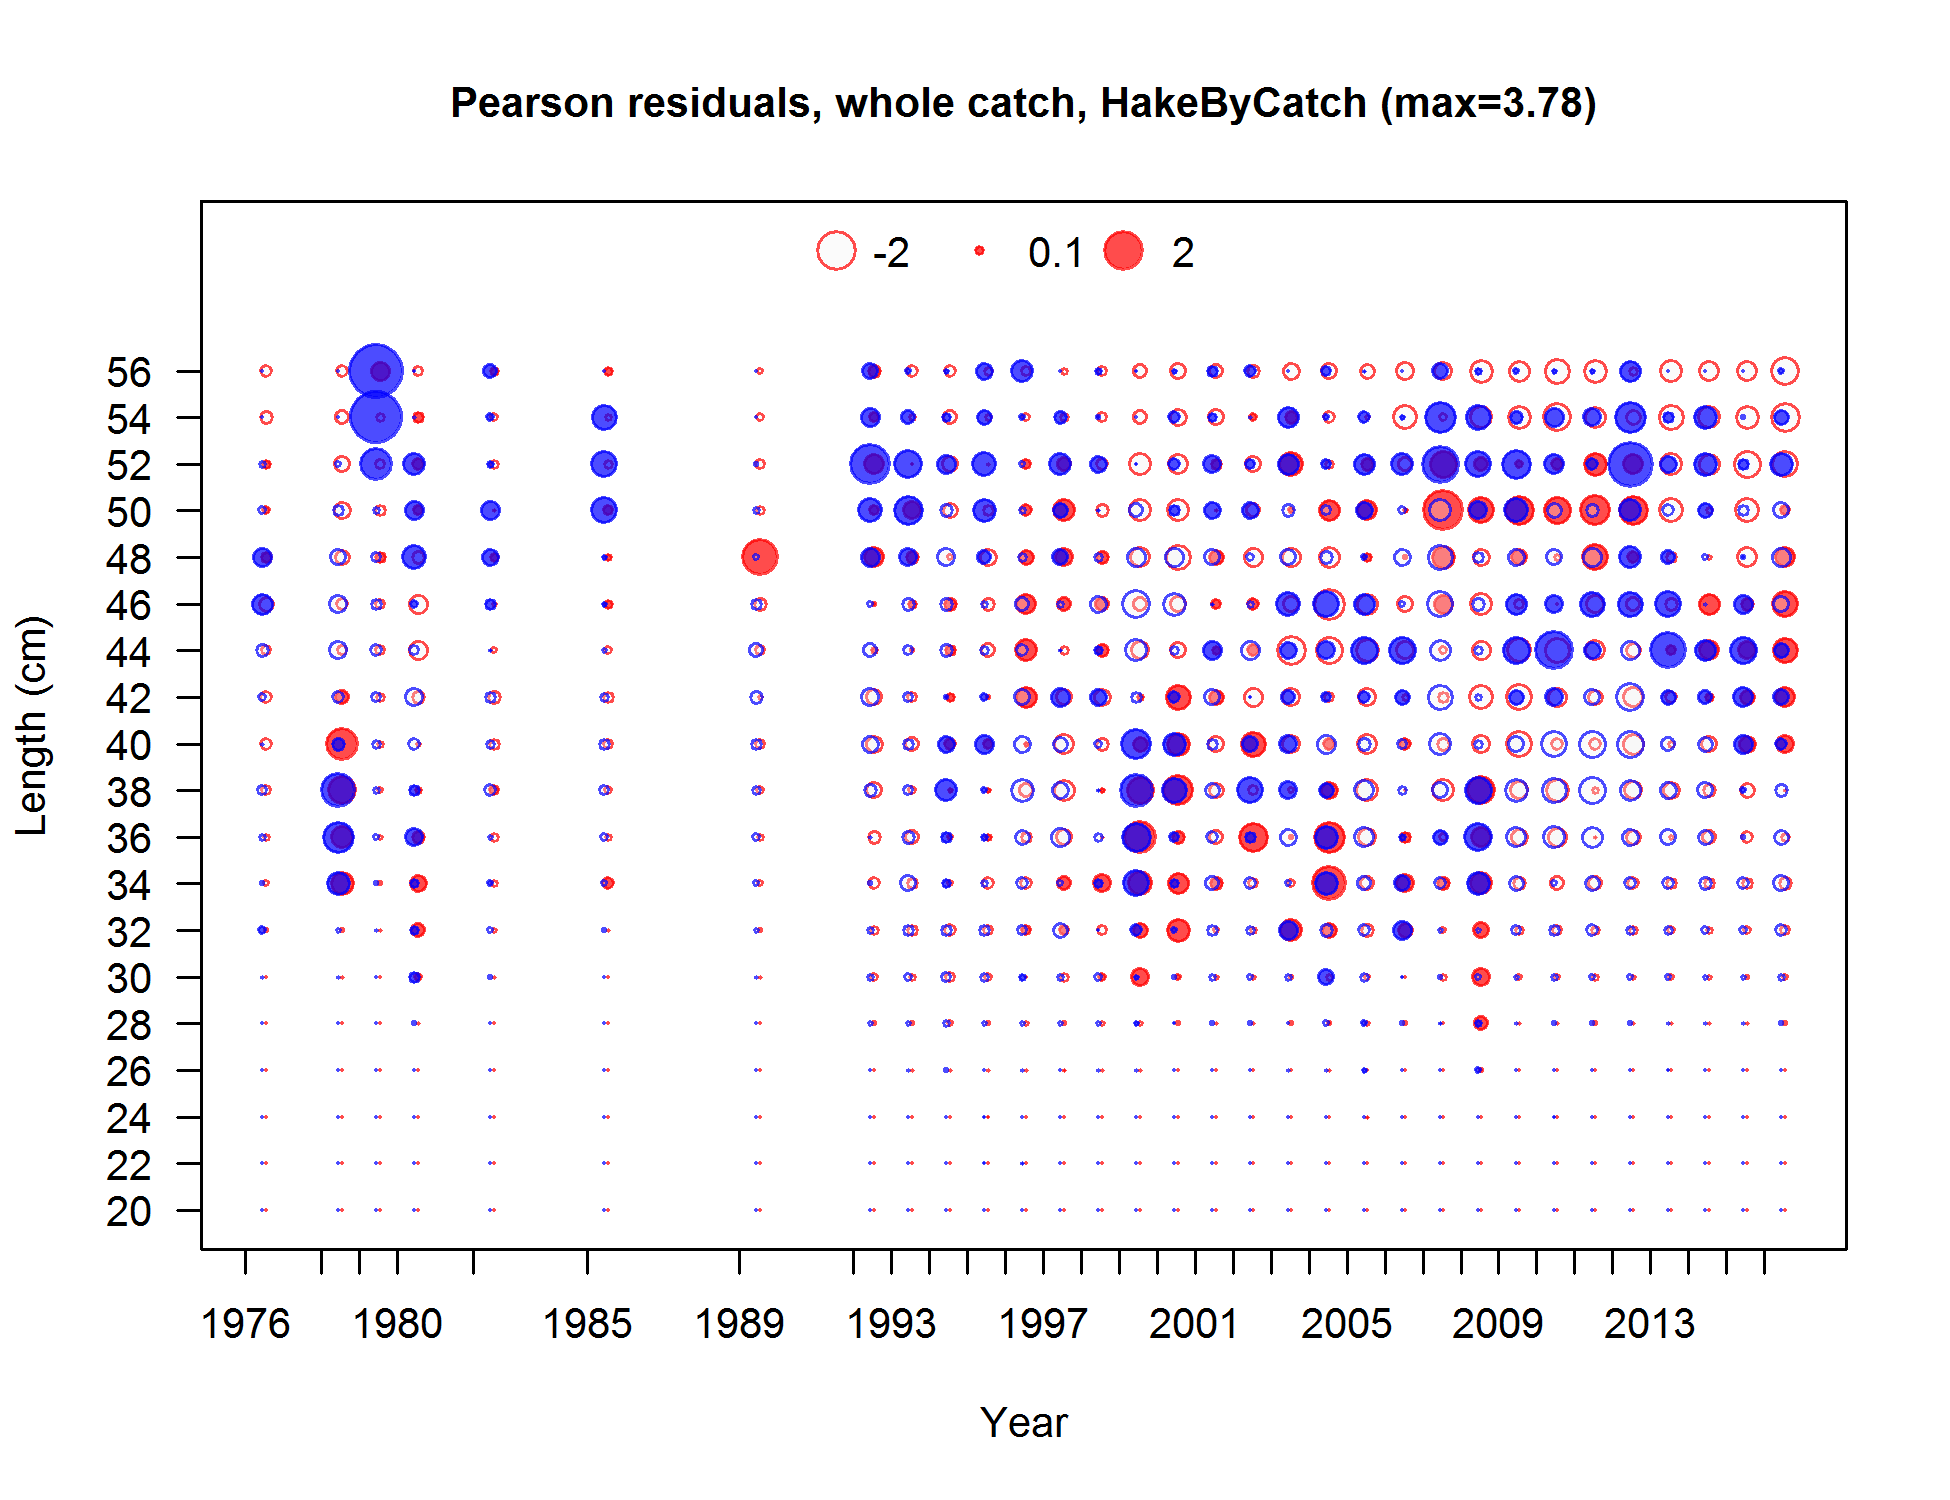
\includegraphics{./r4ss/plots_mod1/comp_lenfit_residsflt2mkt0.png}
\caption{\textbf{Northern model} Pearson residuals, whole catch,
HakeByCatch (max=3.78)\\
Closed bubbles are positive residuals (observed \textgreater{} expected)
and open bubbles are negative residuals (observed \textless{} expected).
\label{fig:mod1_11_comp_lenfit_residsflt2mkt0}}
\end{figure}

\begin{figure}[htbp]
\centering
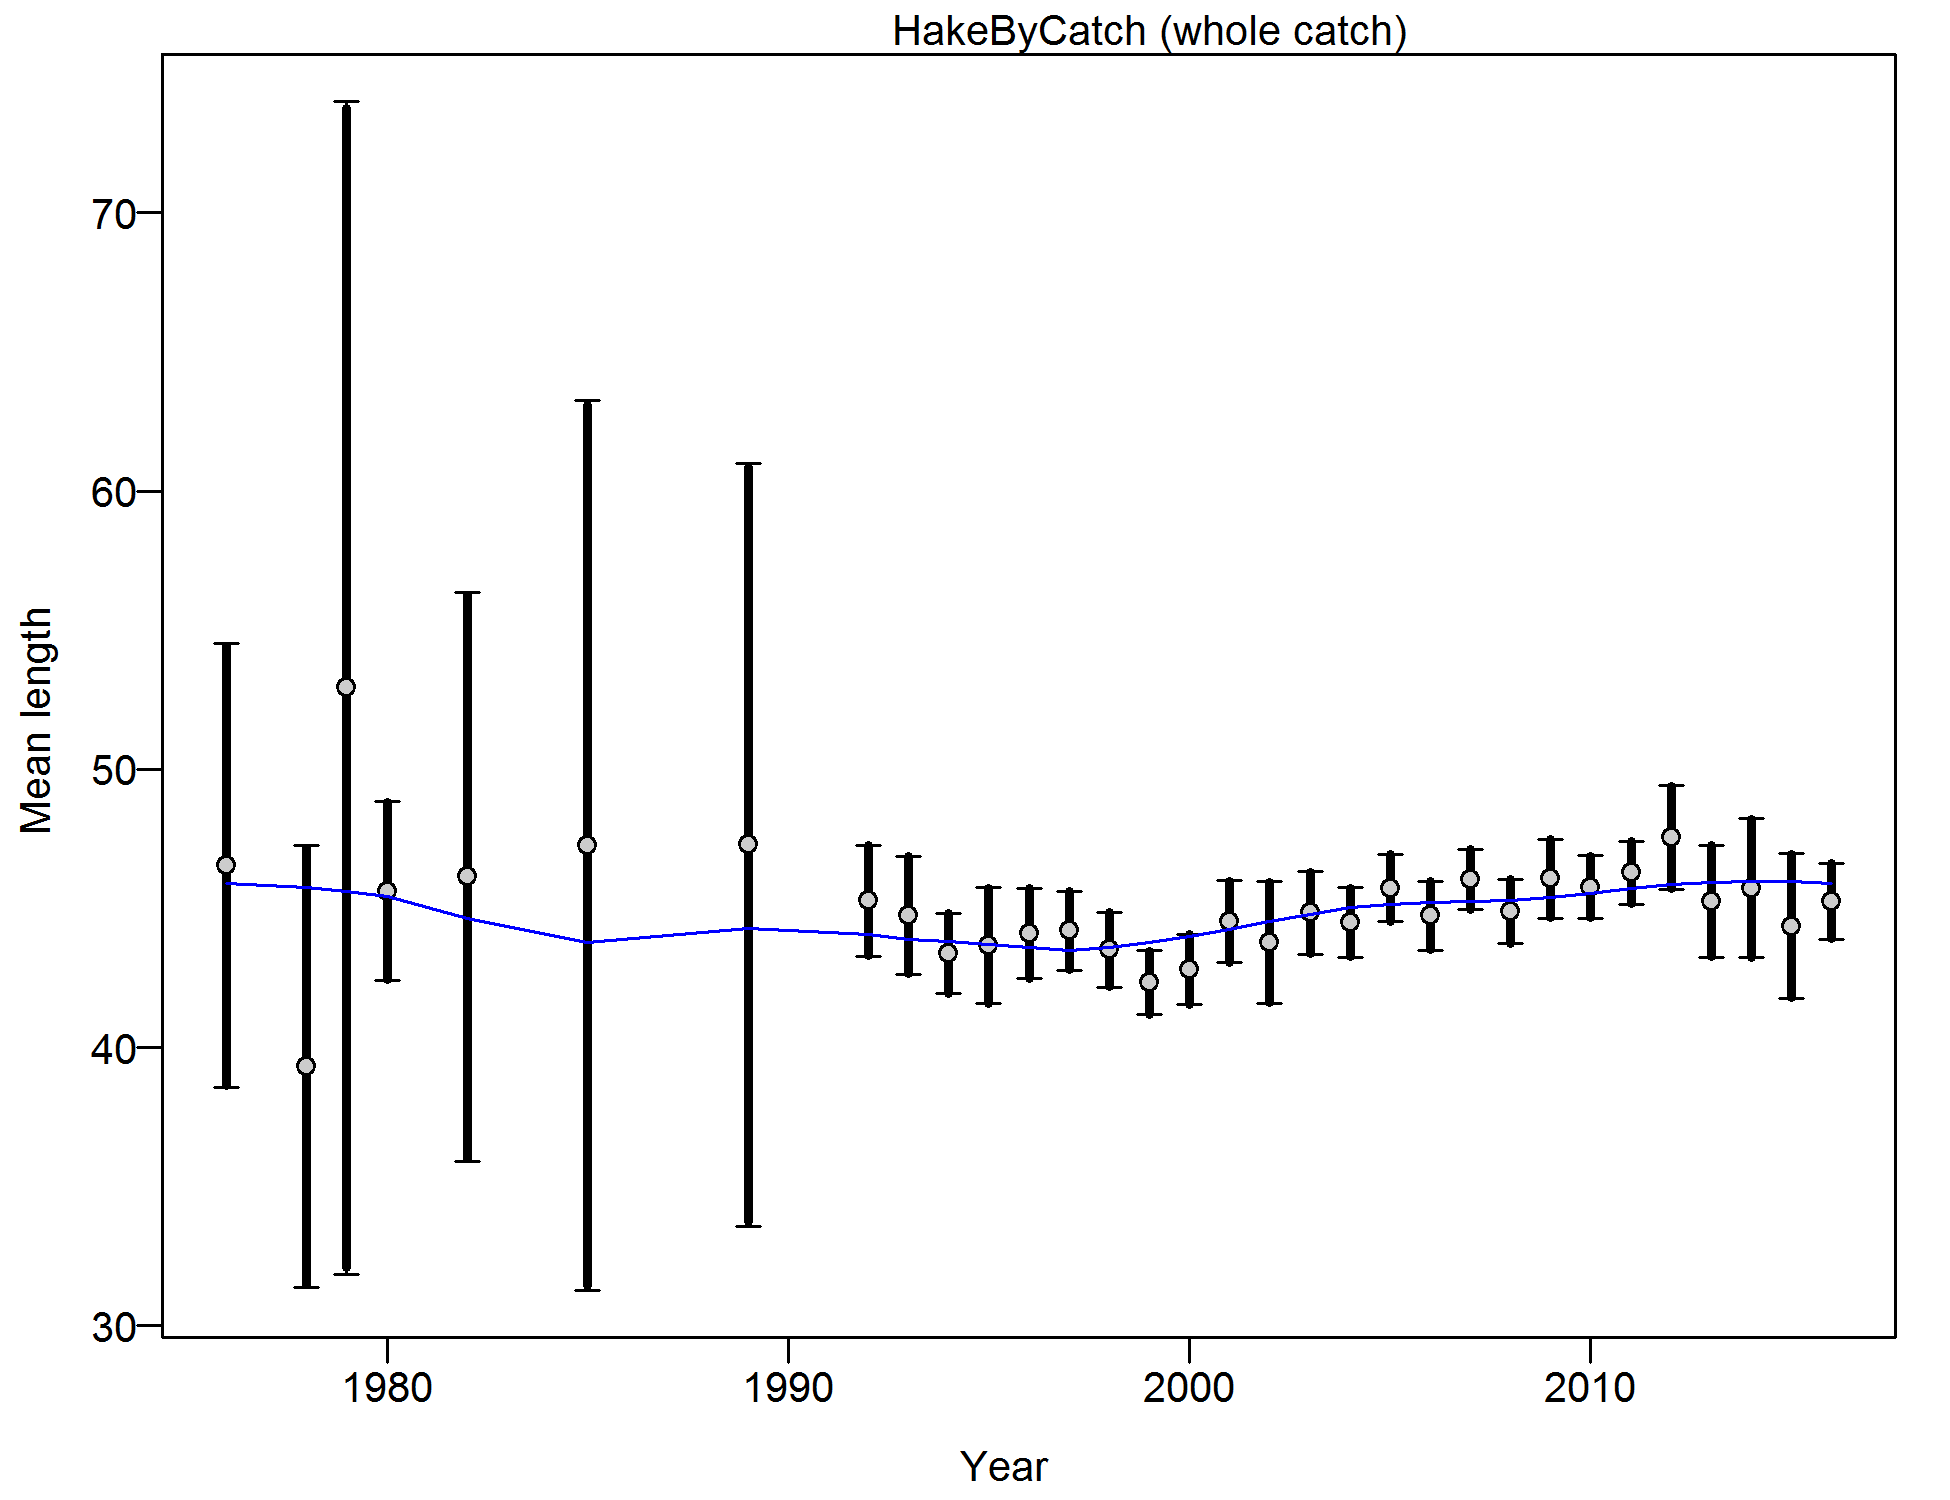
\includegraphics{./r4ss/plots_mod1/comp_lenfit_data_weighting_TA1.8_HakeByCatch.png}
\caption{\textbf{Northern model} Francis data weighting method TA1.8:
HakeByCatch Suggested sample size adjustment (with 95\% interval) for
len data from HakeByCatch: 0.9774 (0.6751\_1.6973) For more info, see
Francis, R.I.C.C. (2011). Data weighting in statistical fisheries stock
assessment models. Can. J. Fish. Aquat. Sci. 68: 1124\_1138.
\label{fig:mod1_13_comp_lenfit_data_weighting_TA1.8_HakeByCatch}}
\end{figure}

\begin{figure}[htbp]
\centering
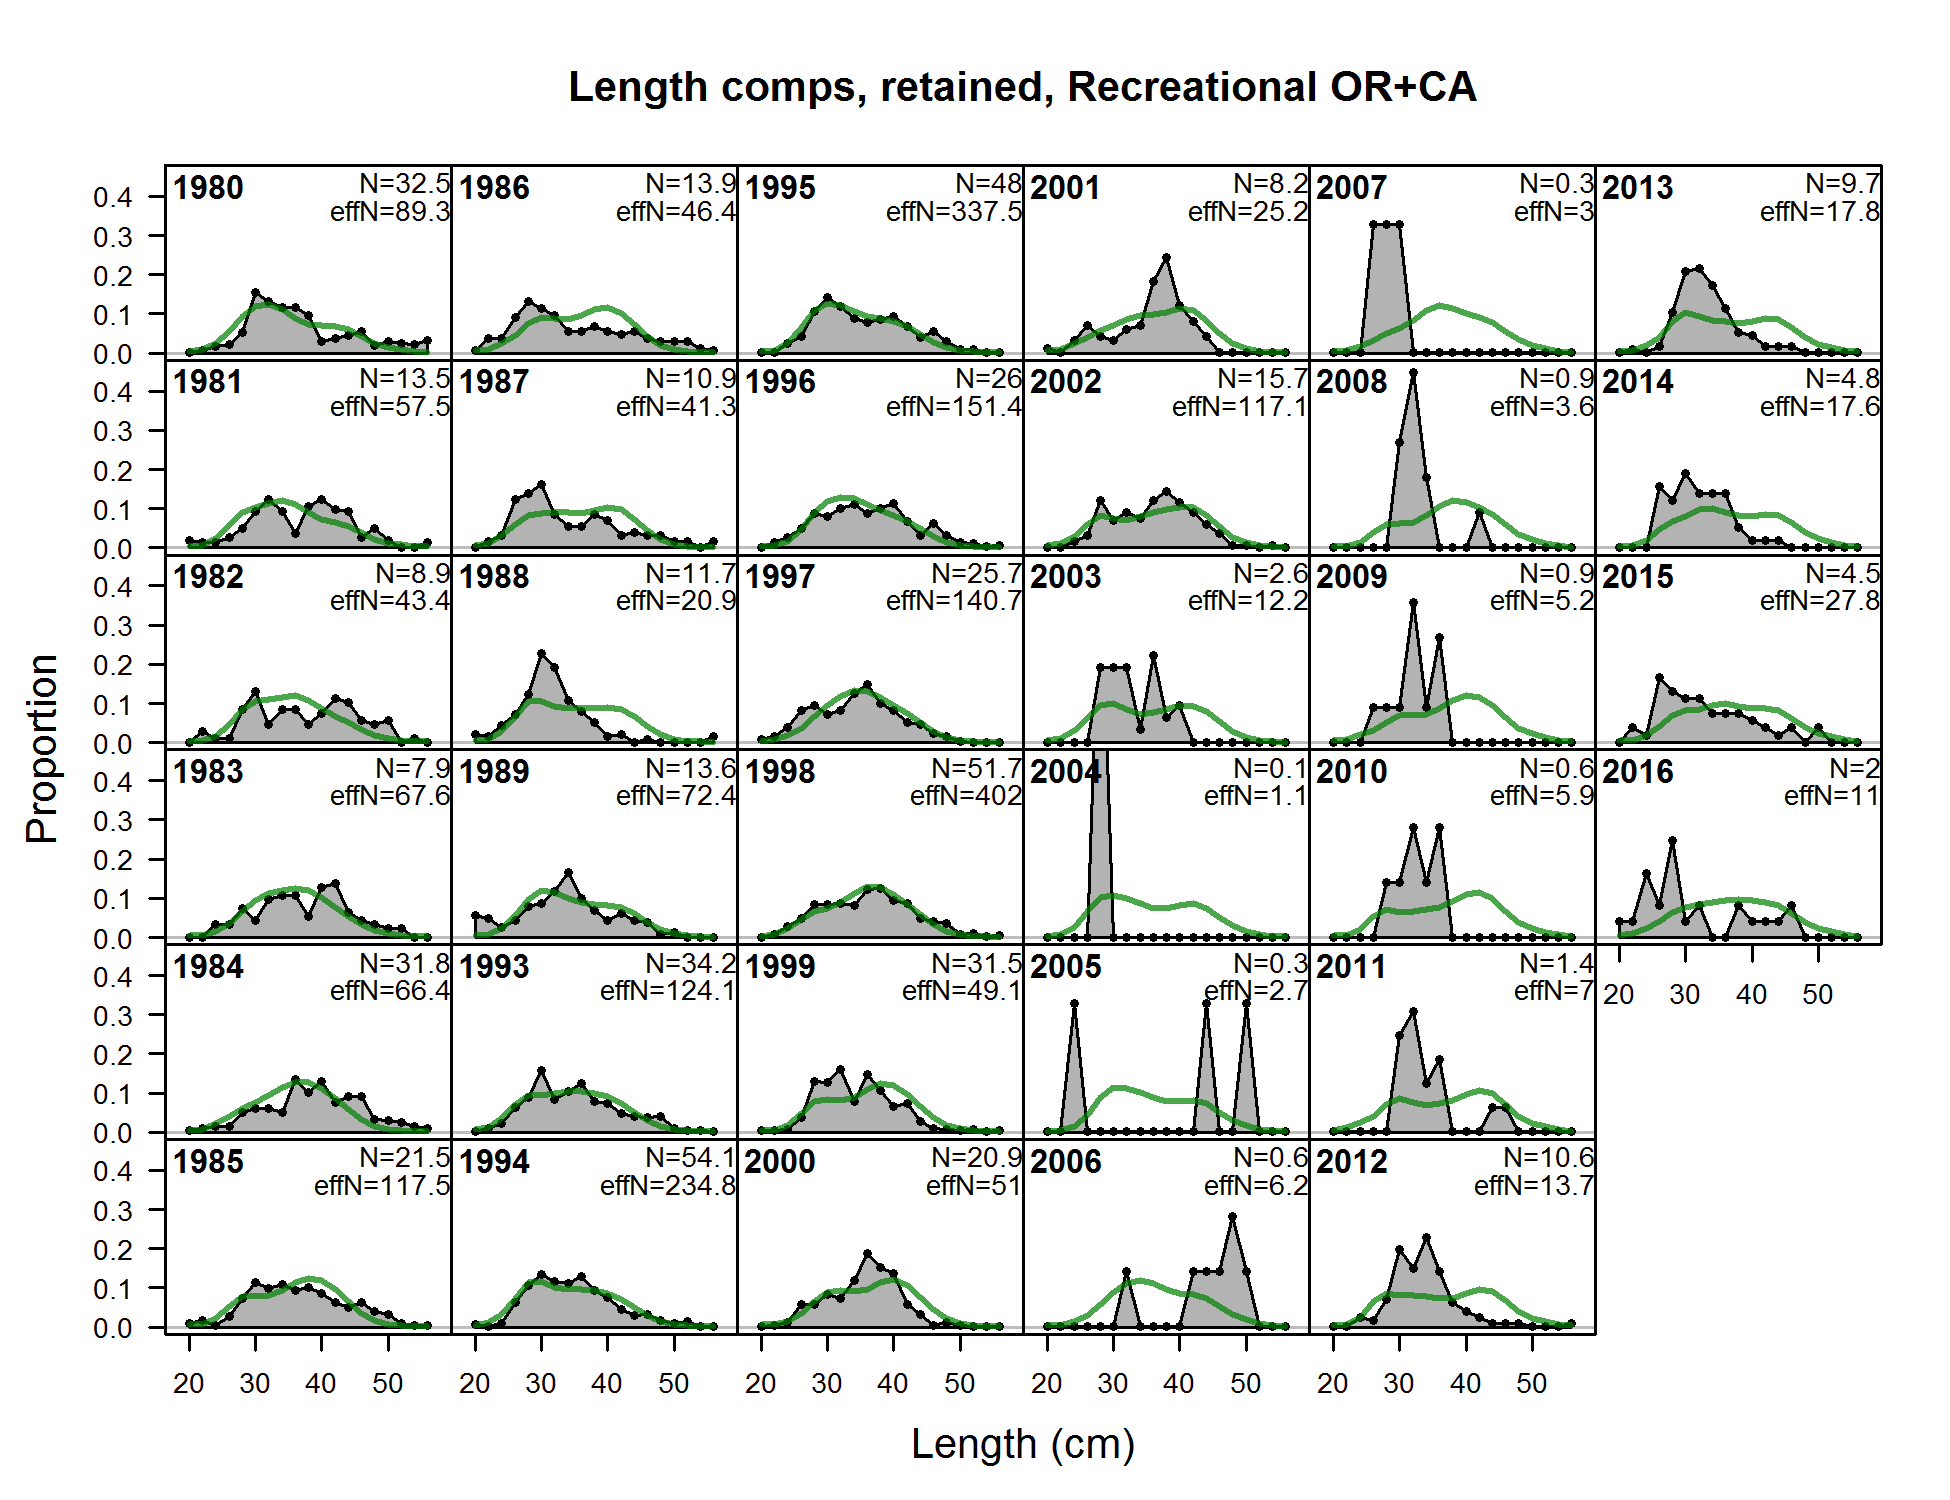
\includegraphics{./r4ss/plots_mod1/comp_lenfit_flt3mkt2.png}
\caption{\textbf{Northern model} Length comps, retained, RecORandCA
\label{fig:mod1_14_comp_lenfit_flt3mkt2}}
\end{figure}

\begin{figure}[htbp]
\centering
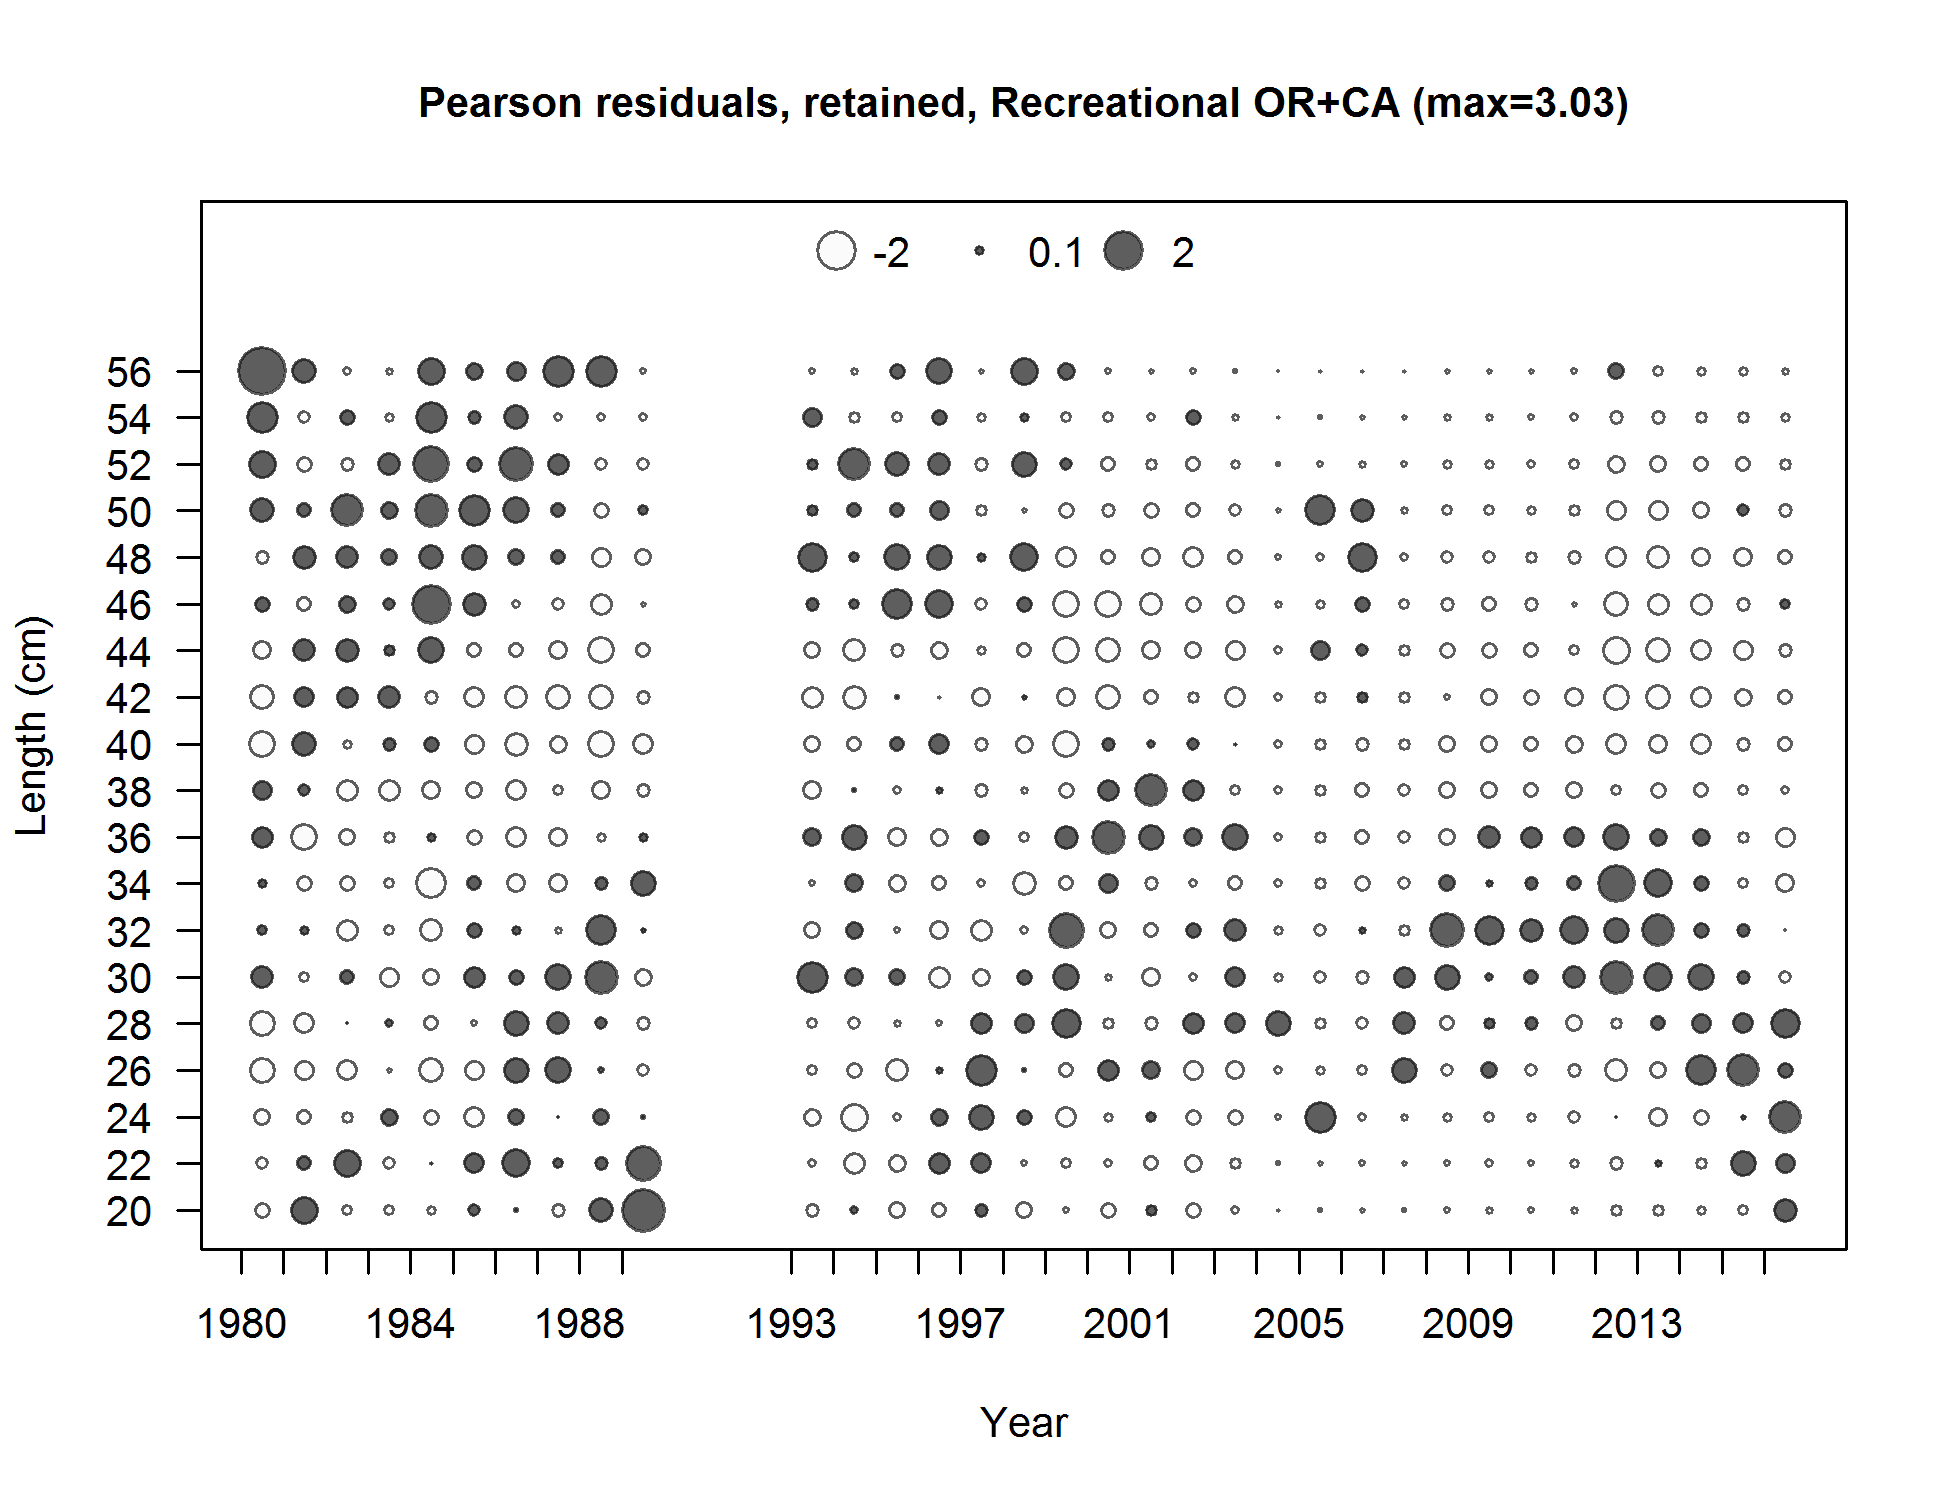
\includegraphics{./r4ss/plots_mod1/comp_lenfit_residsflt3mkt2.png}
\caption{\textbf{Northern model} Pearson residuals, retained, RecORandCA
(max=3.03)\\
Closed bubbles are positive residuals (observed \textgreater{} expected)
and open bubbles are negative residuals (observed \textless{} expected).
\label{fig:mod1_15_comp_lenfit_residsflt3mkt2}}
\end{figure}

\begin{figure}[htbp]
\centering
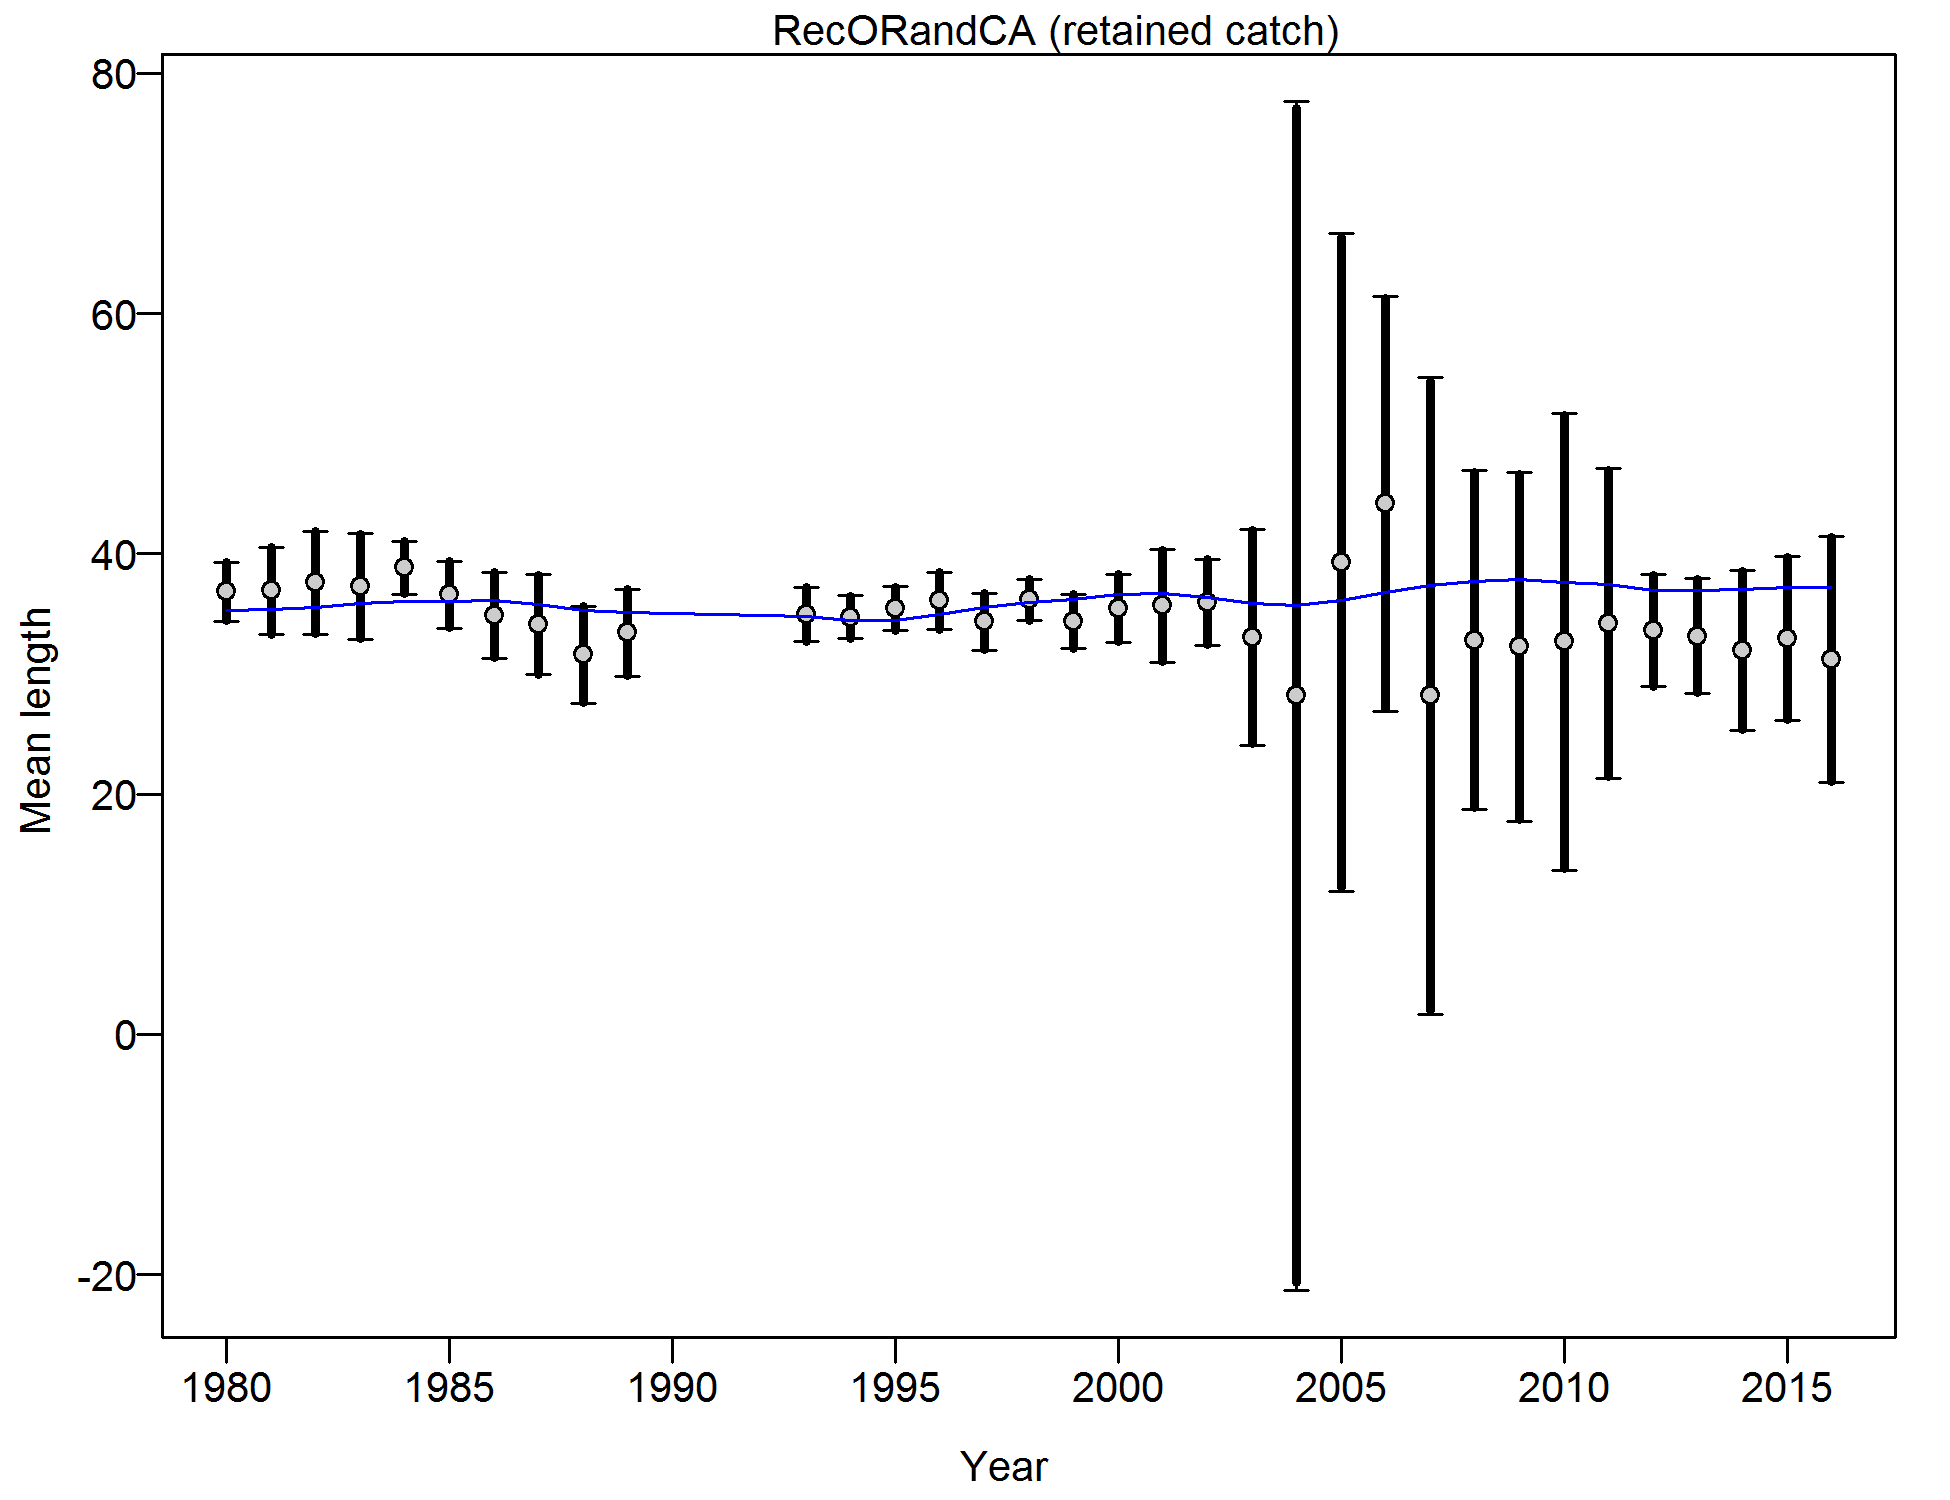
\includegraphics{./r4ss/plots_mod1/comp_lenfit_data_weighting_TA1.8_RecORandCA.png}
\caption{\textbf{Northern model} Francis data weighting method TA1.8:
RecORandCA Suggested sample size adjustment (with 95\% interval) for len
data from RecORandCA: 0.9761 (0.6621\_1.774) For more info, see Francis,
R.I.C.C. (2011). Data weighting in statistical fisheries stock
assessment models. Can. J. Fish. Aquat. Sci. 68: 1124\_1138.
\label{fig:mod1_17_comp_lenfit_data_weighting_TA1.8_RecORandCA}}
\end{figure}

\begin{figure}[htbp]
\centering
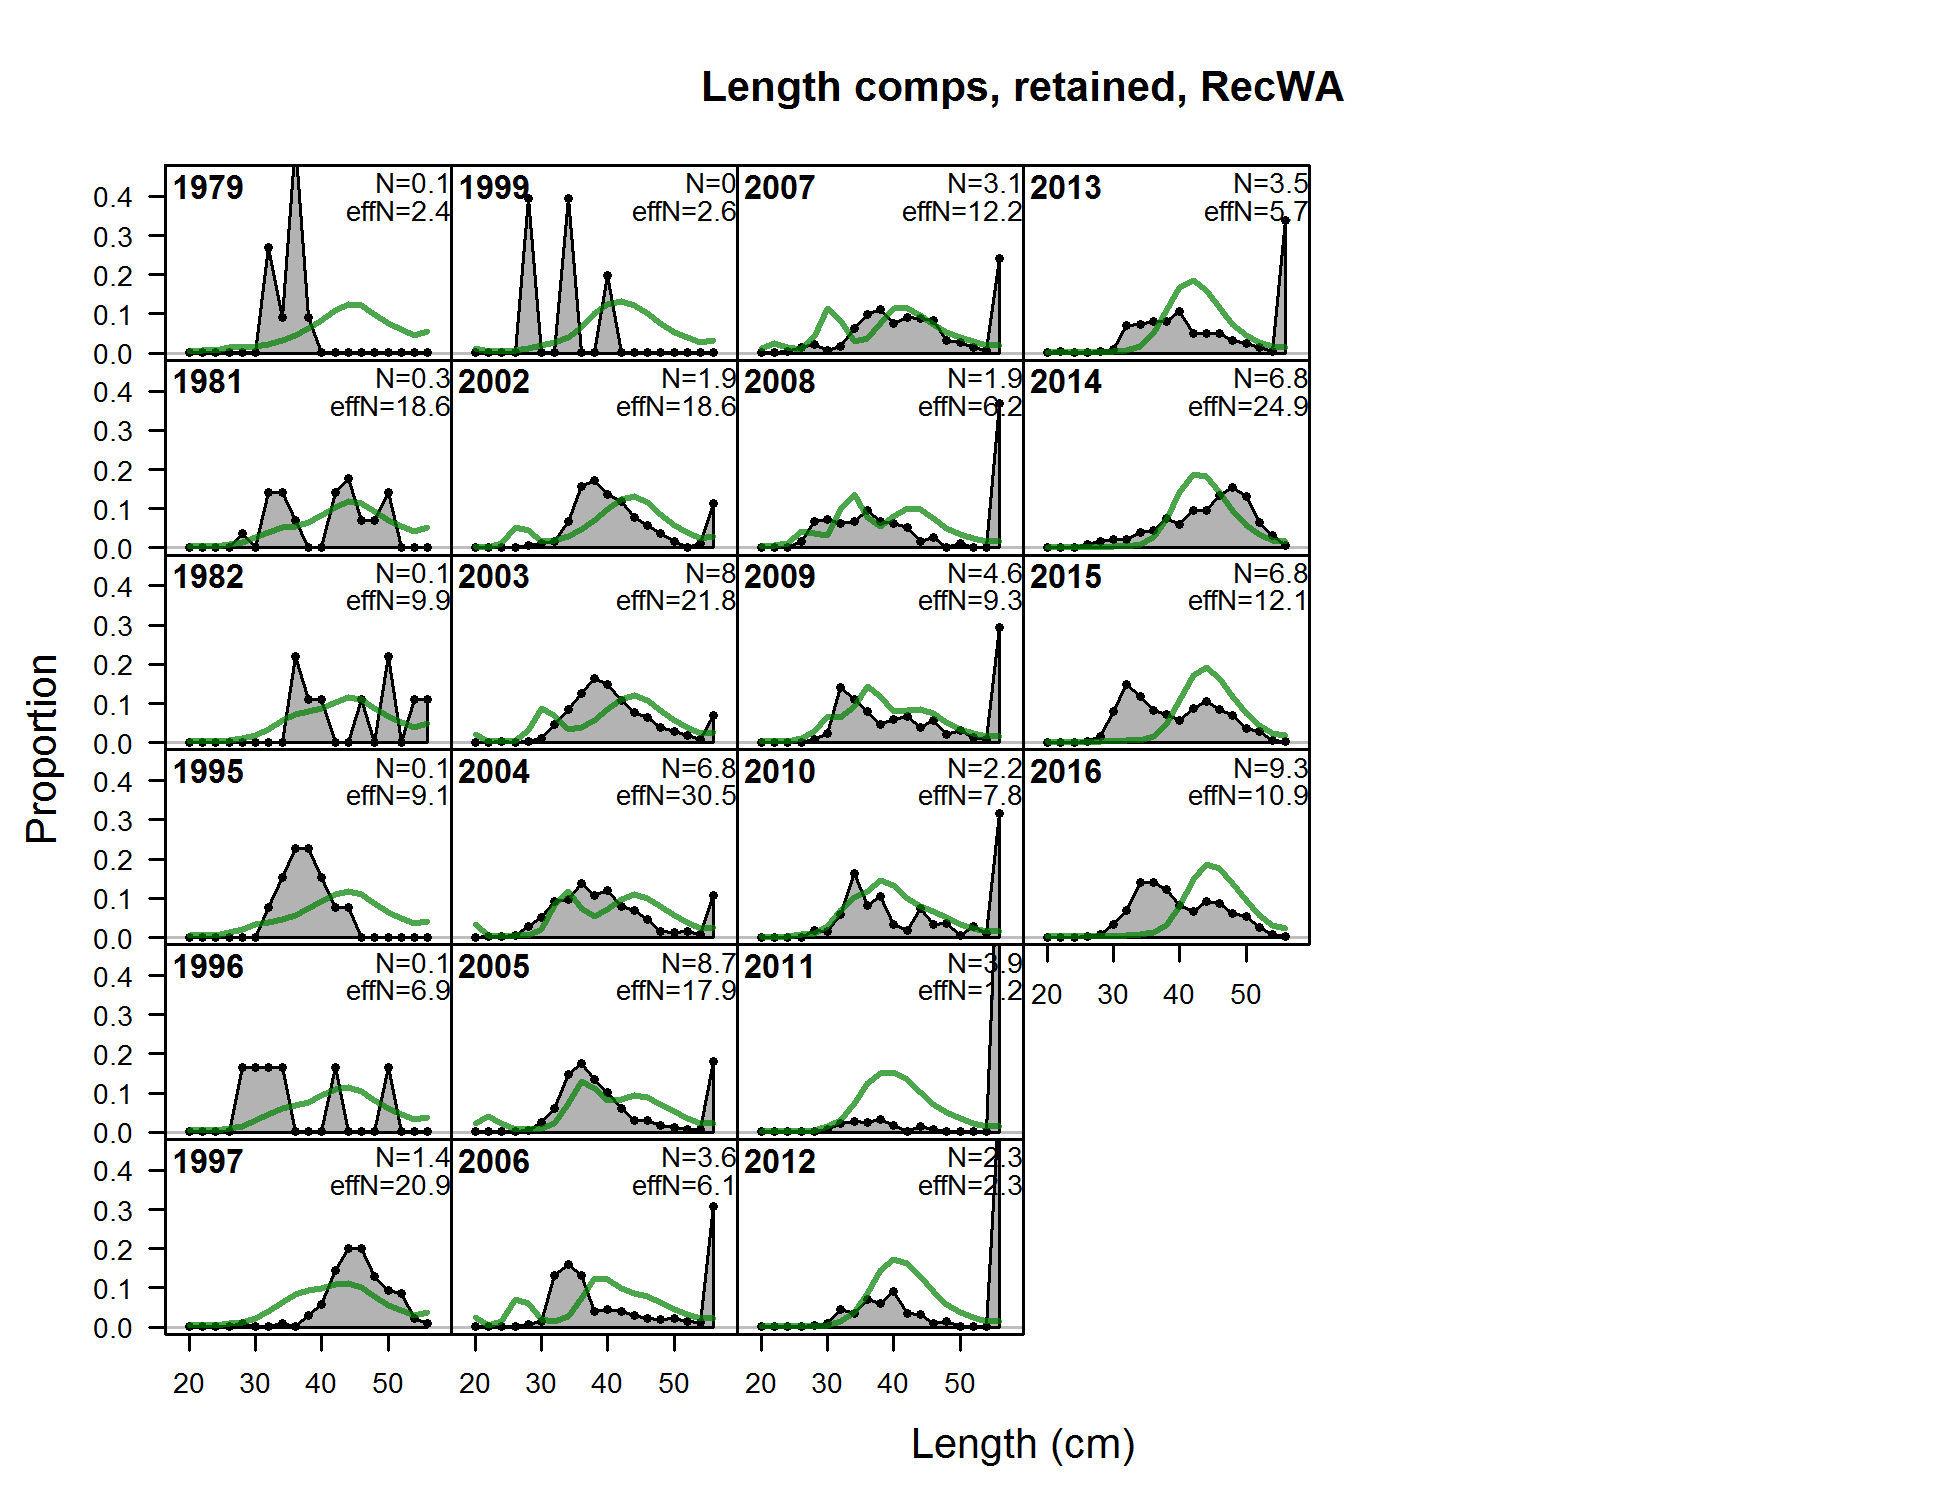
\includegraphics{./r4ss/plots_mod1/comp_lenfit_flt4mkt2.png}
\caption{\textbf{Northern model} Length comps, retained, RecWA
\label{fig:mod1_18_comp_lenfit_flt4mkt2}}
\end{figure}

\begin{figure}[htbp]
\centering
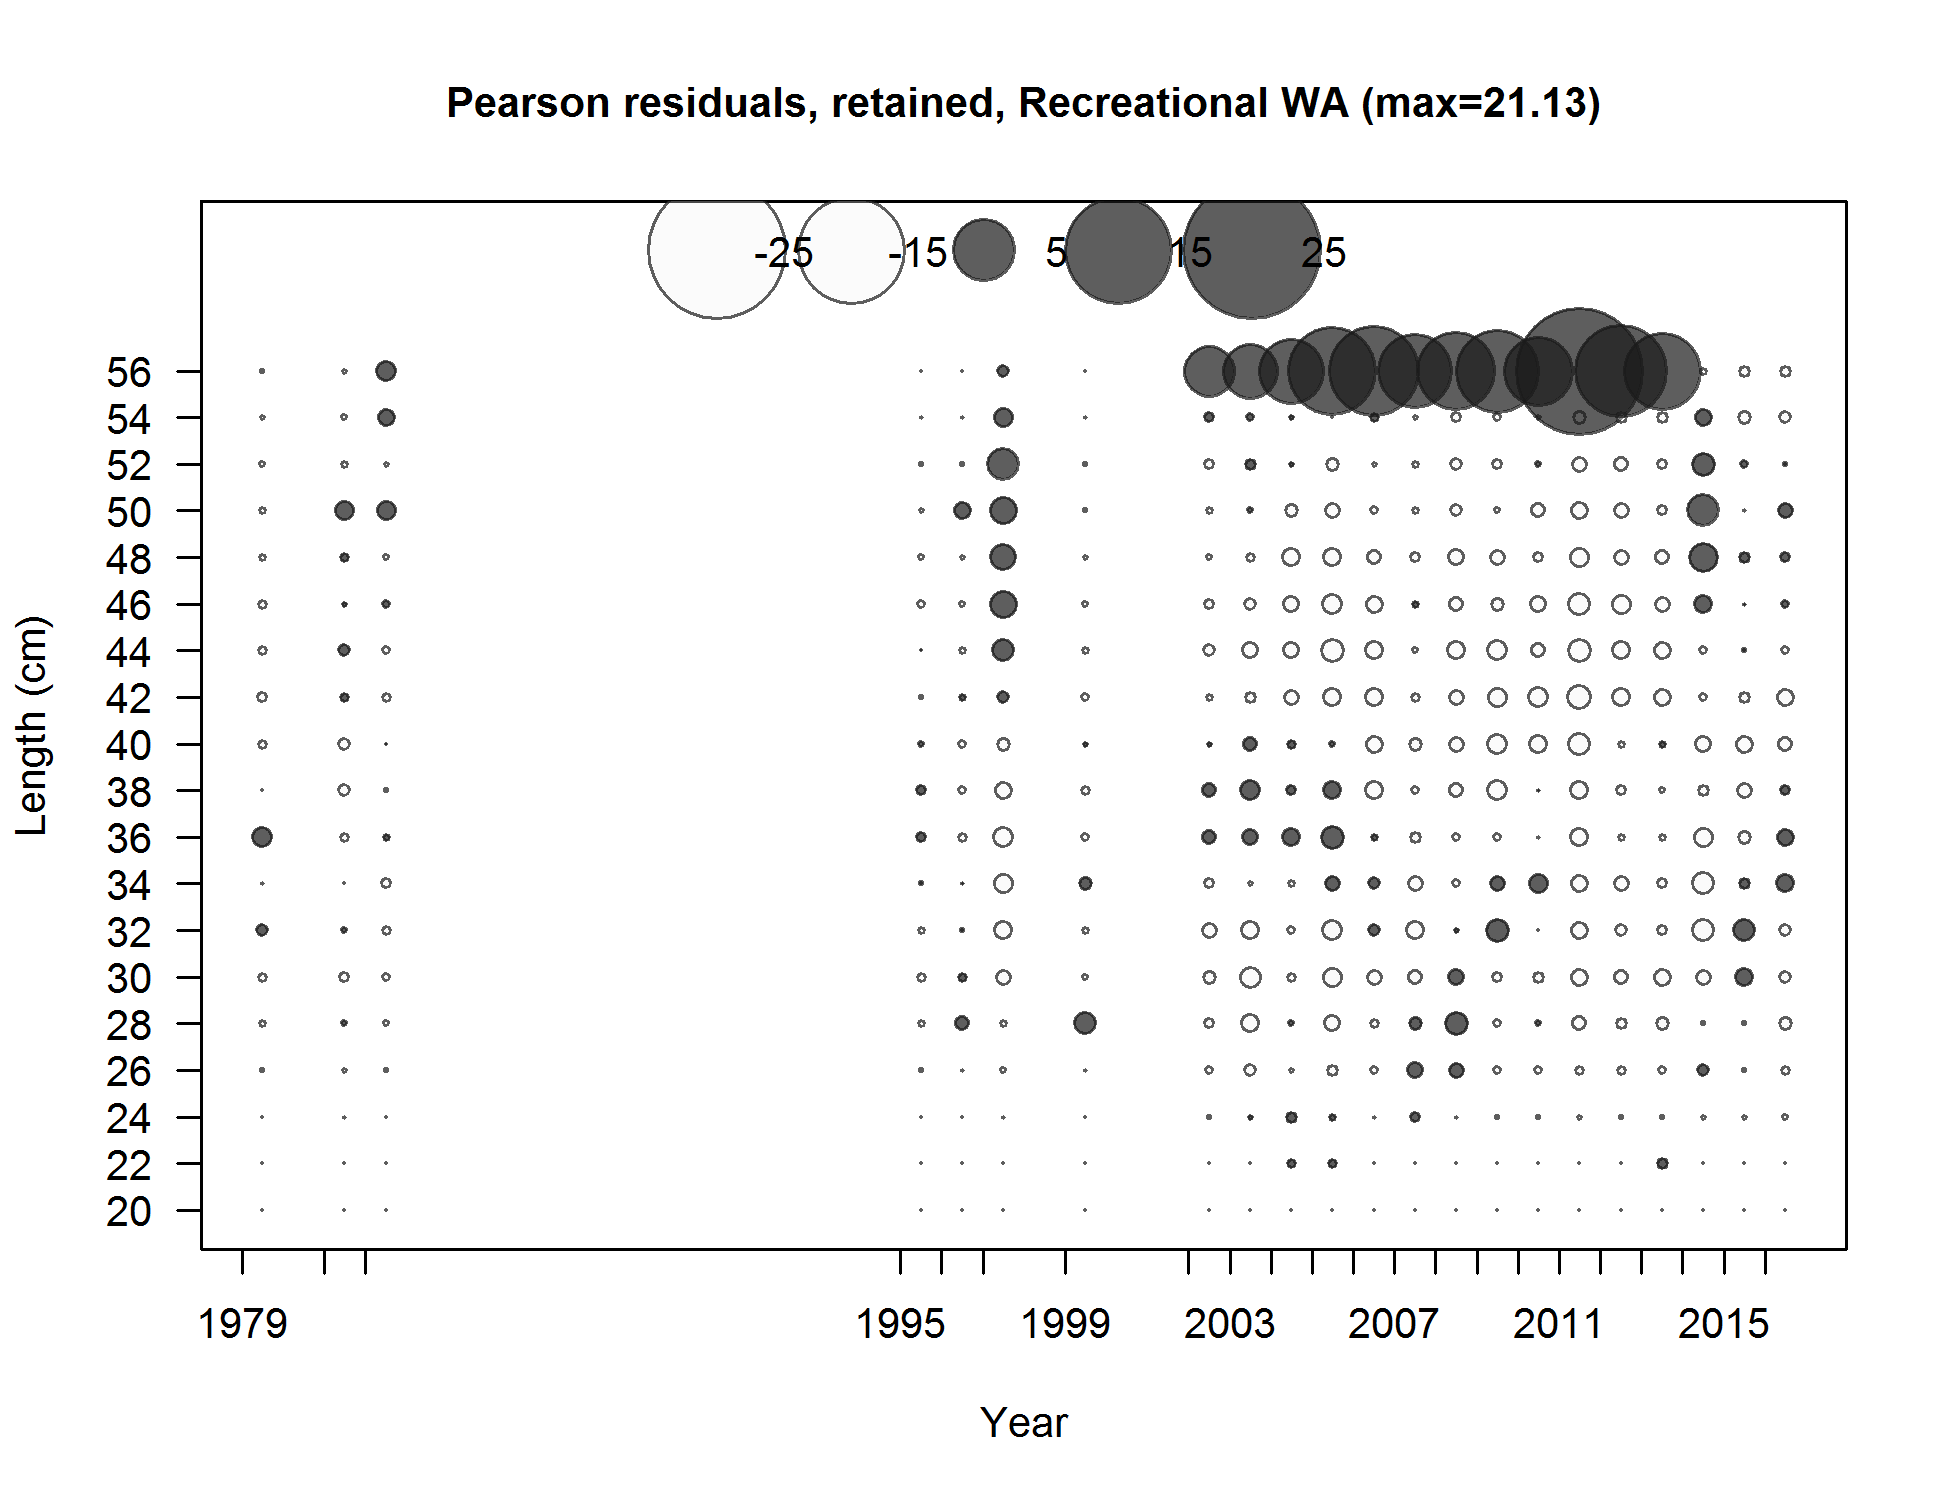
\includegraphics{./r4ss/plots_mod1/comp_lenfit_residsflt4mkt2.png}
\caption{\textbf{Northern model} Pearson residuals, retained, RecWA
(max=23.16)\\
Closed bubbles are positive residuals (observed \textgreater{} expected)
and open bubbles are negative residuals (observed \textless{} expected).
\label{fig:mod1_19_comp_lenfit_residsflt4mkt2}}
\end{figure}

\begin{figure}[htbp]
\centering
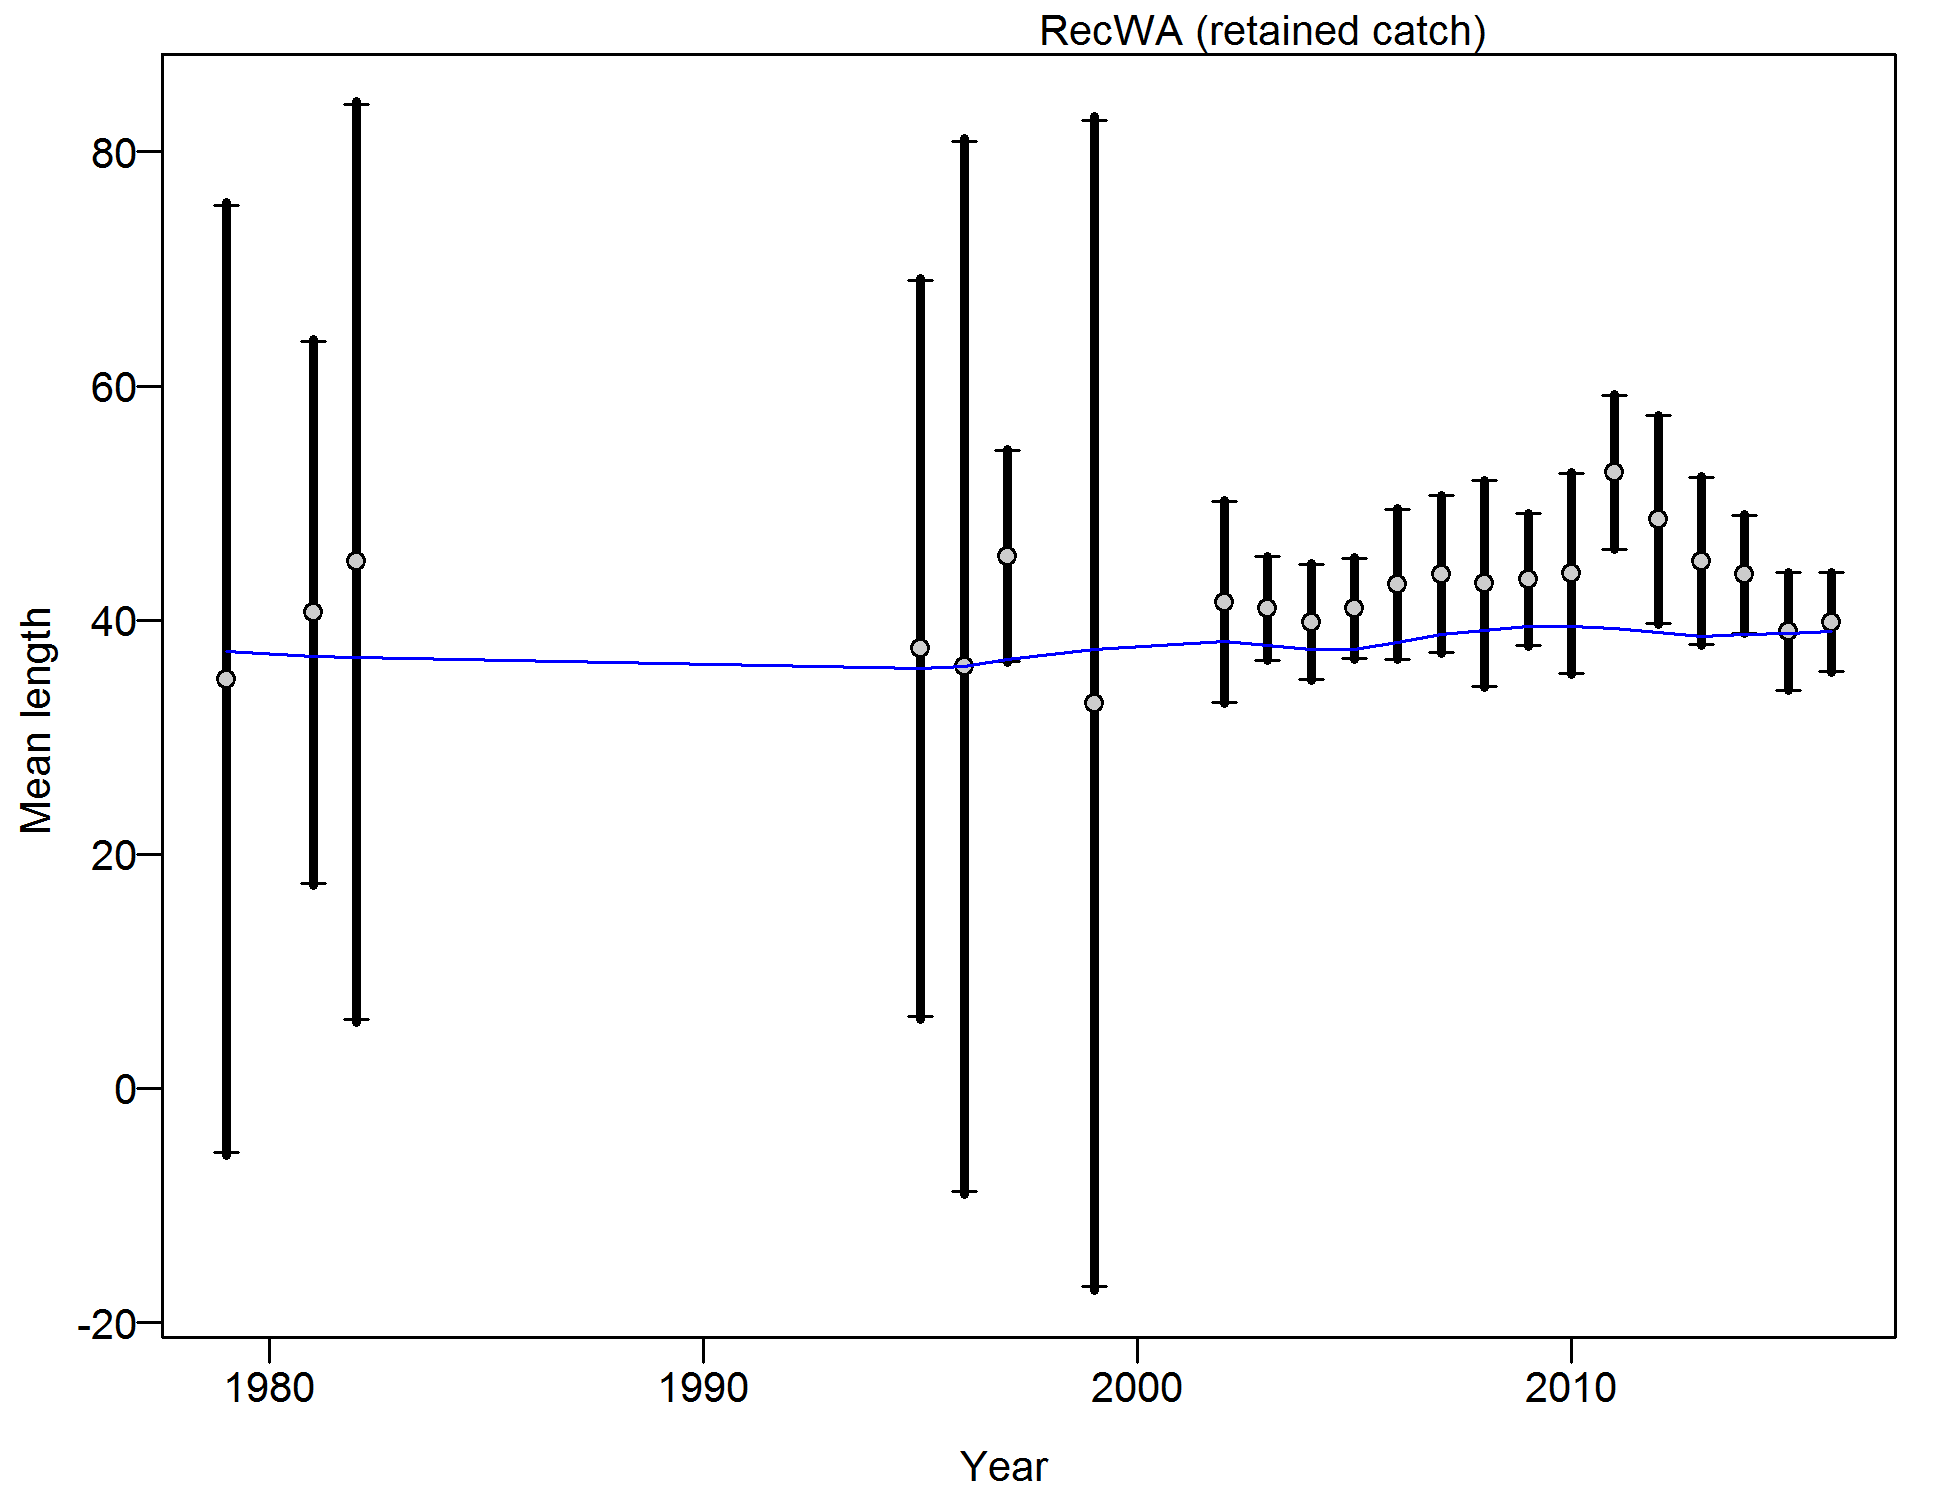
\includegraphics{./r4ss/plots_mod1/comp_lenfit_data_weighting_TA1.8_RecWA.png}
\caption{\textbf{Northern model} Francis data weighting method TA1.8:
RecWA Suggested sample size adjustment (with 95\% interval) for len data
from RecWA: 1.0134 (0.5588\_2.3419) For more info, see Francis, R.I.C.C.
(2011). Data weighting in statistical fisheries stock assessment models.
Can. J. Fish. Aquat. Sci. 68: 1124\_1138.
\label{fig:mod1_21_comp_lenfit_data_weighting_TA1.8_RecWA}}
\end{figure}

\begin{figure}[htbp]
\centering
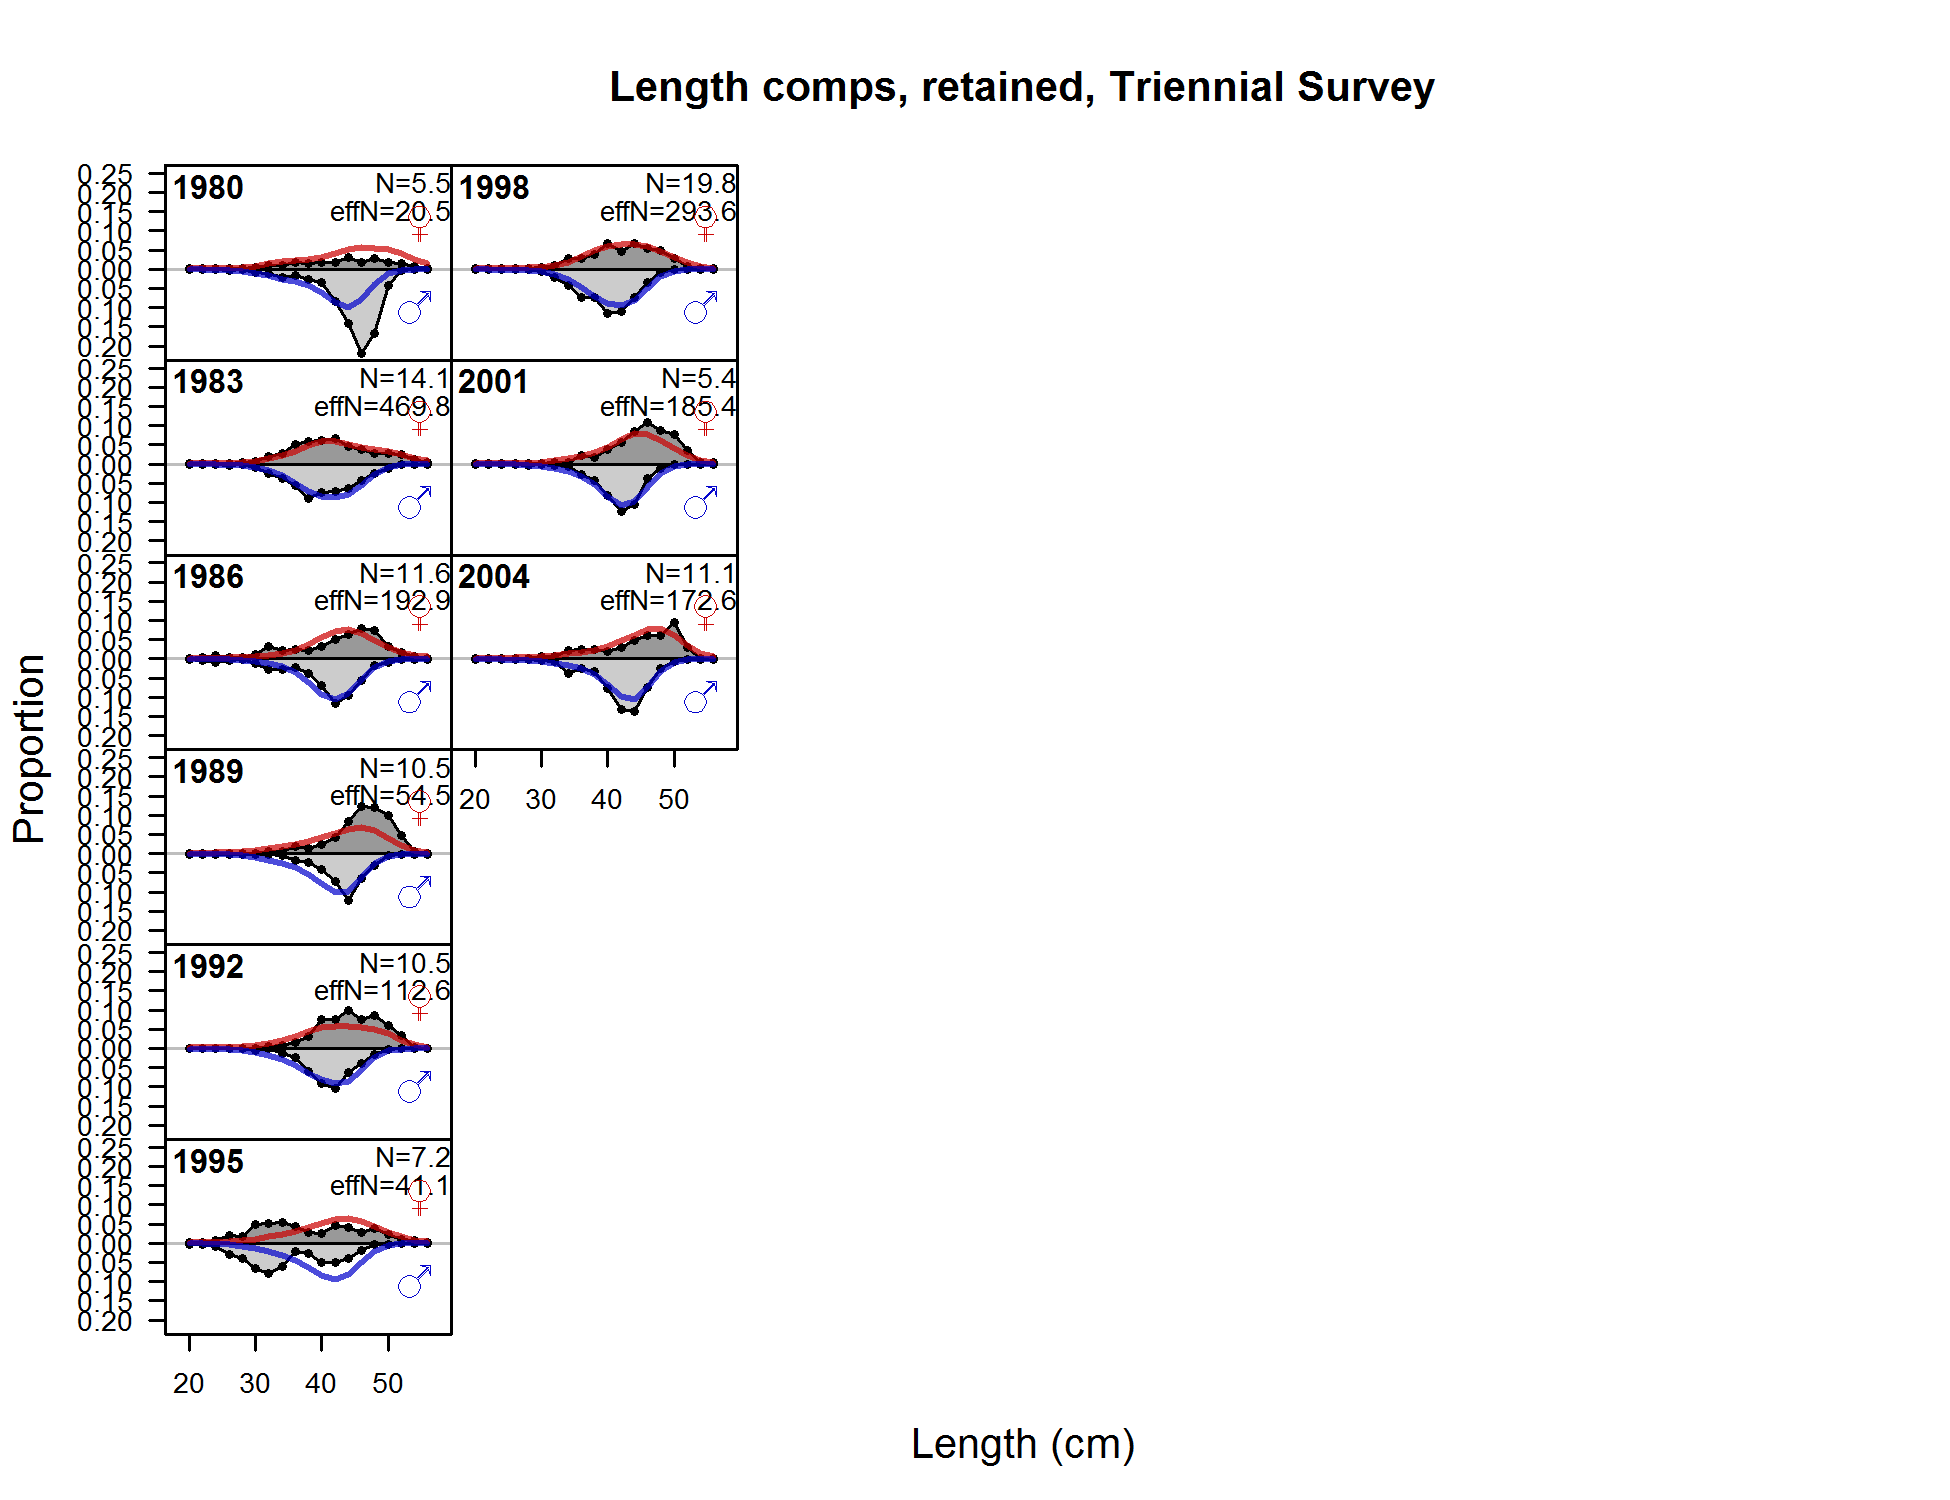
\includegraphics{./r4ss/plots_mod1/comp_lenfit_flt5mkt2.png}
\caption{\textbf{Northern model} Length comps, retained, Triennial
\label{fig:mod1_22_comp_lenfit_flt5mkt2}}
\end{figure}

\begin{figure}[htbp]
\centering
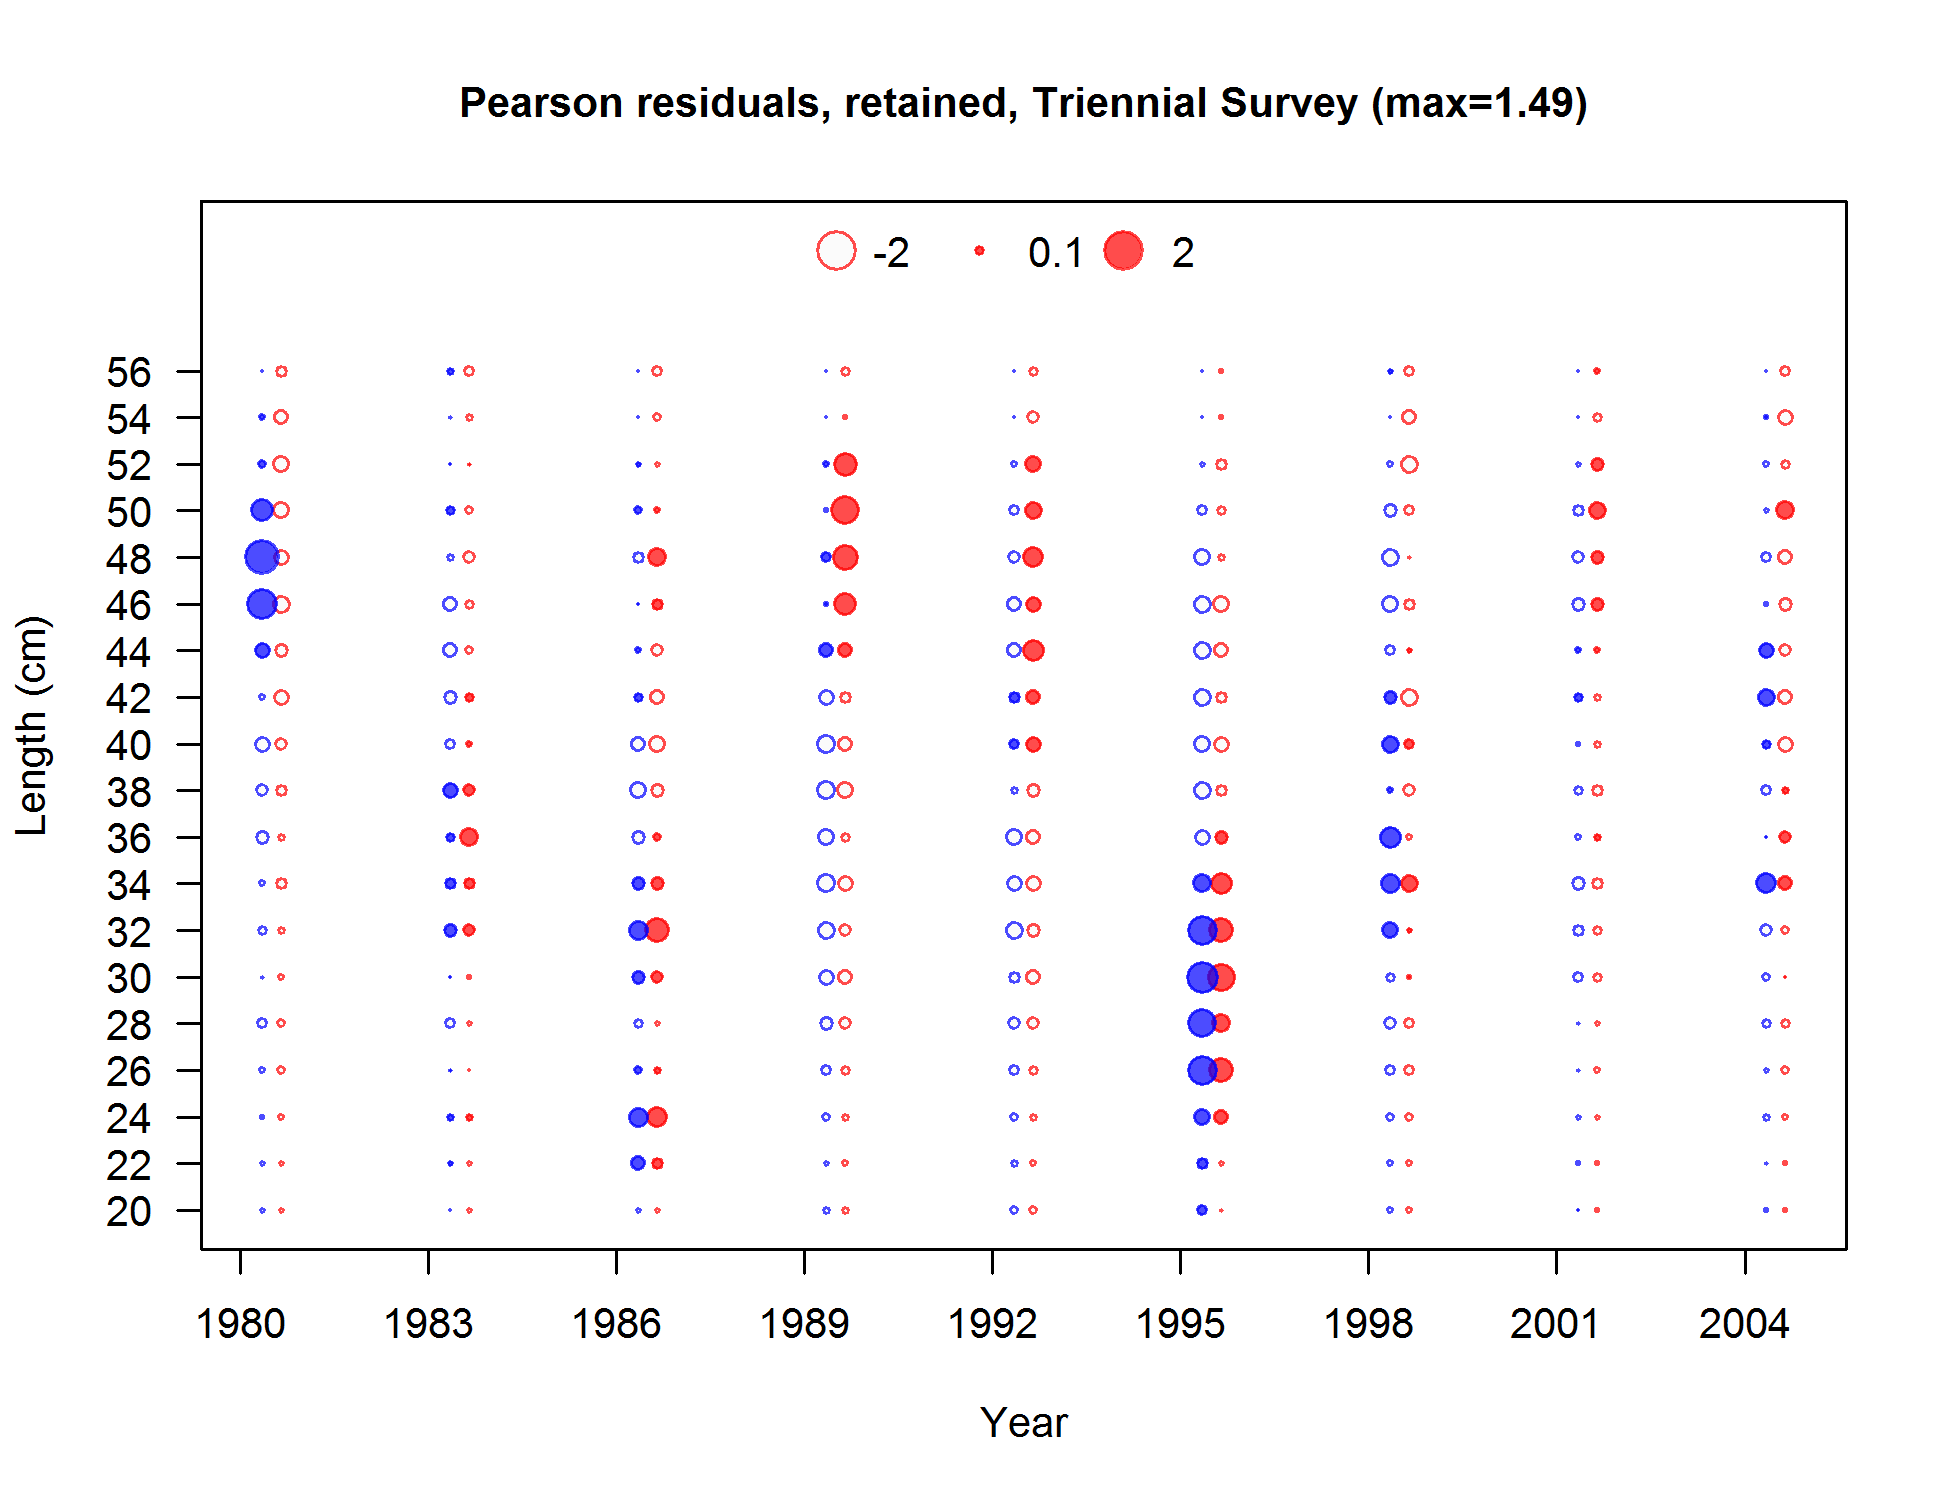
\includegraphics{./r4ss/plots_mod1/comp_lenfit_residsflt5mkt2.png}
\caption{\textbf{Northern model} Pearson residuals, retained, Triennial
(max=1.54)\\
Closed bubbles are positive residuals (observed \textgreater{} expected)
and open bubbles are negative residuals (observed \textless{} expected).
\label{fig:mod1_23_comp_lenfit_residsflt5mkt2}}
\end{figure}

\begin{figure}[htbp]
\centering
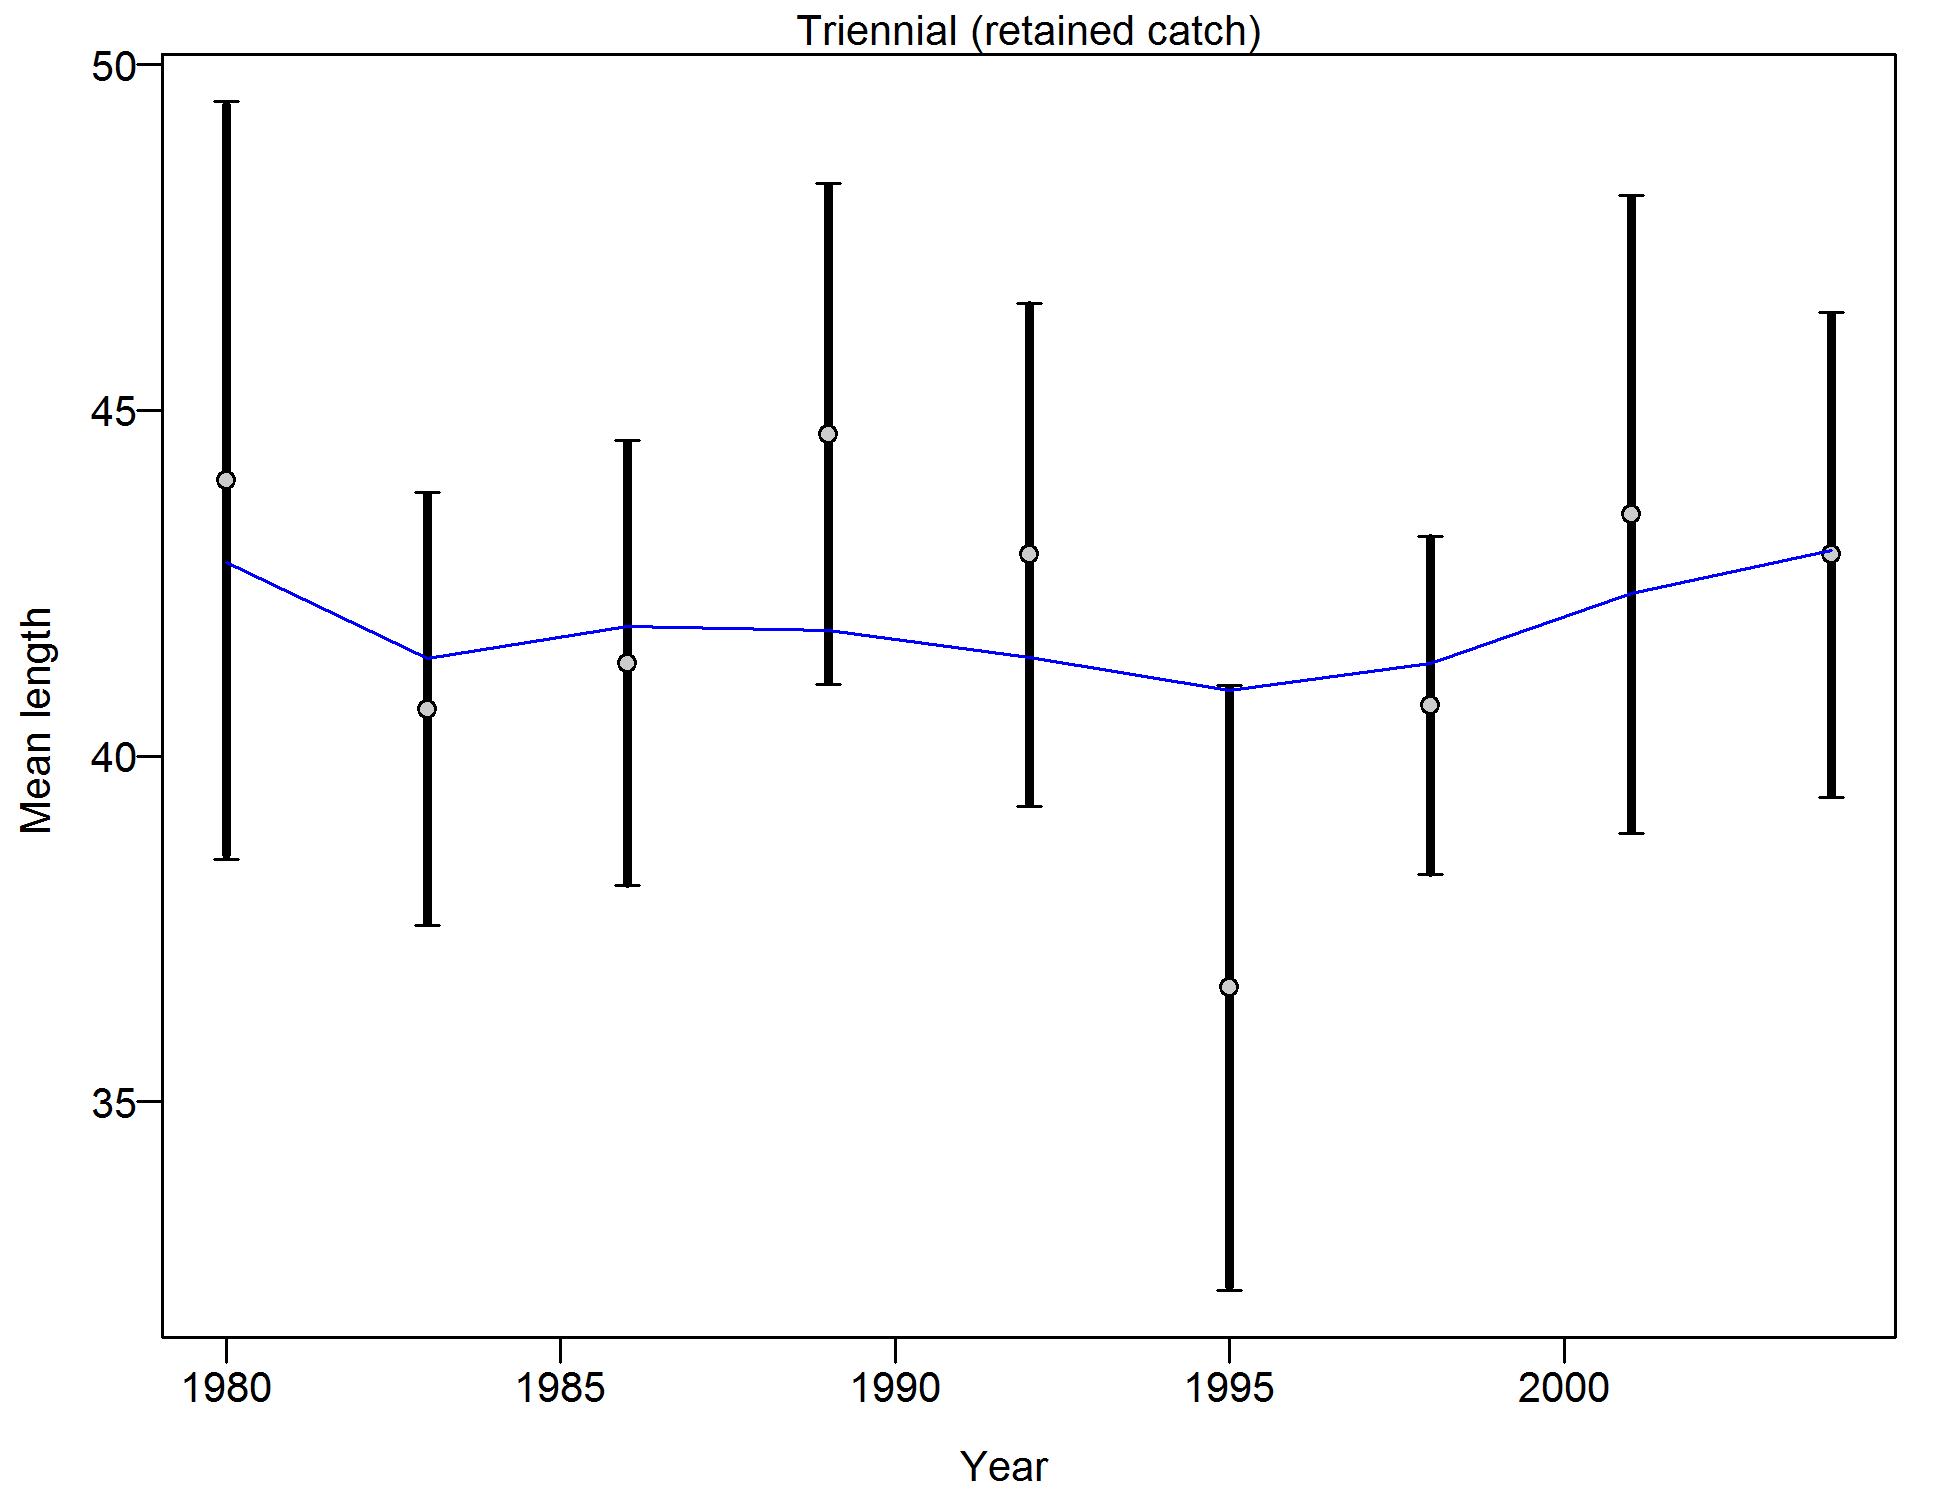
\includegraphics{./r4ss/plots_mod1/comp_lenfit_data_weighting_TA1.8_Triennial.png}
\caption{\textbf{Northern model} Francis data weighting method TA1.8:
Triennial Suggested sample size adjustment (with 95\% interval) for len
data from Triennial: 0.9781 (0.5131\_5.1969) For more info, see Francis,
R.I.C.C. (2011). Data weighting in statistical fisheries stock
assessment models. Can. J. Fish. Aquat. Sci. 68: 1124\_1138.
\label{fig:mod1_25_comp_lenfit_data_weighting_TA1.8_Triennial}}
\end{figure}

\begin{figure}[htbp]
\centering
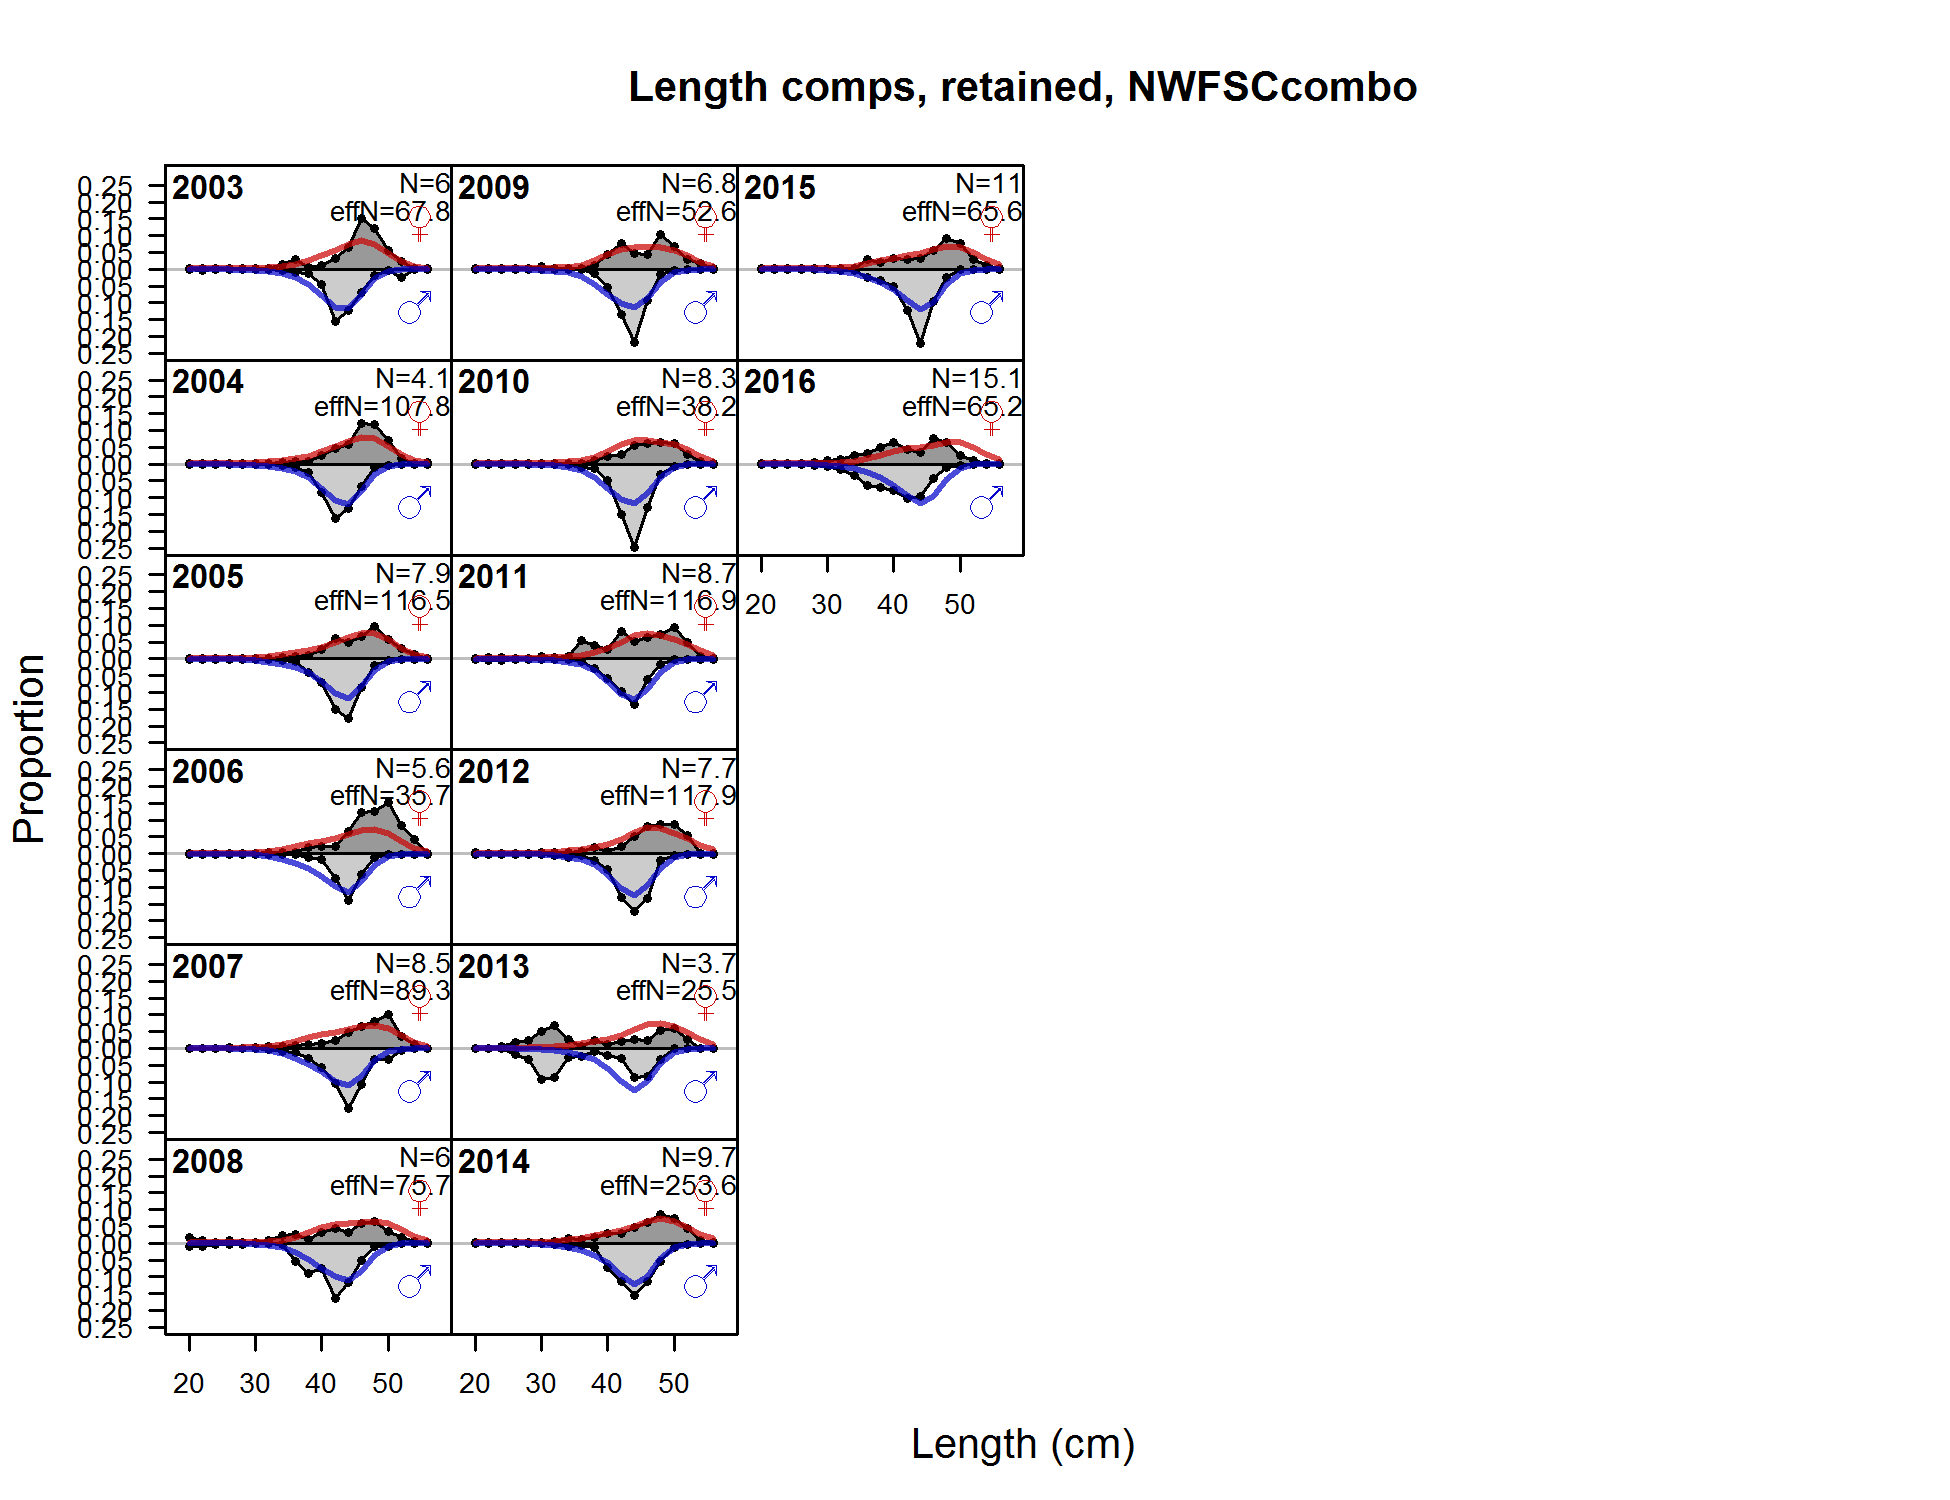
\includegraphics{./r4ss/plots_mod1/comp_lenfit_flt6mkt2.png}
\caption{\textbf{Northern model} Length comps, retained, NWFSCcombo
\label{fig:mod1_26_comp_lenfit_flt6mkt2}}
\end{figure}

\begin{figure}[htbp]
\centering
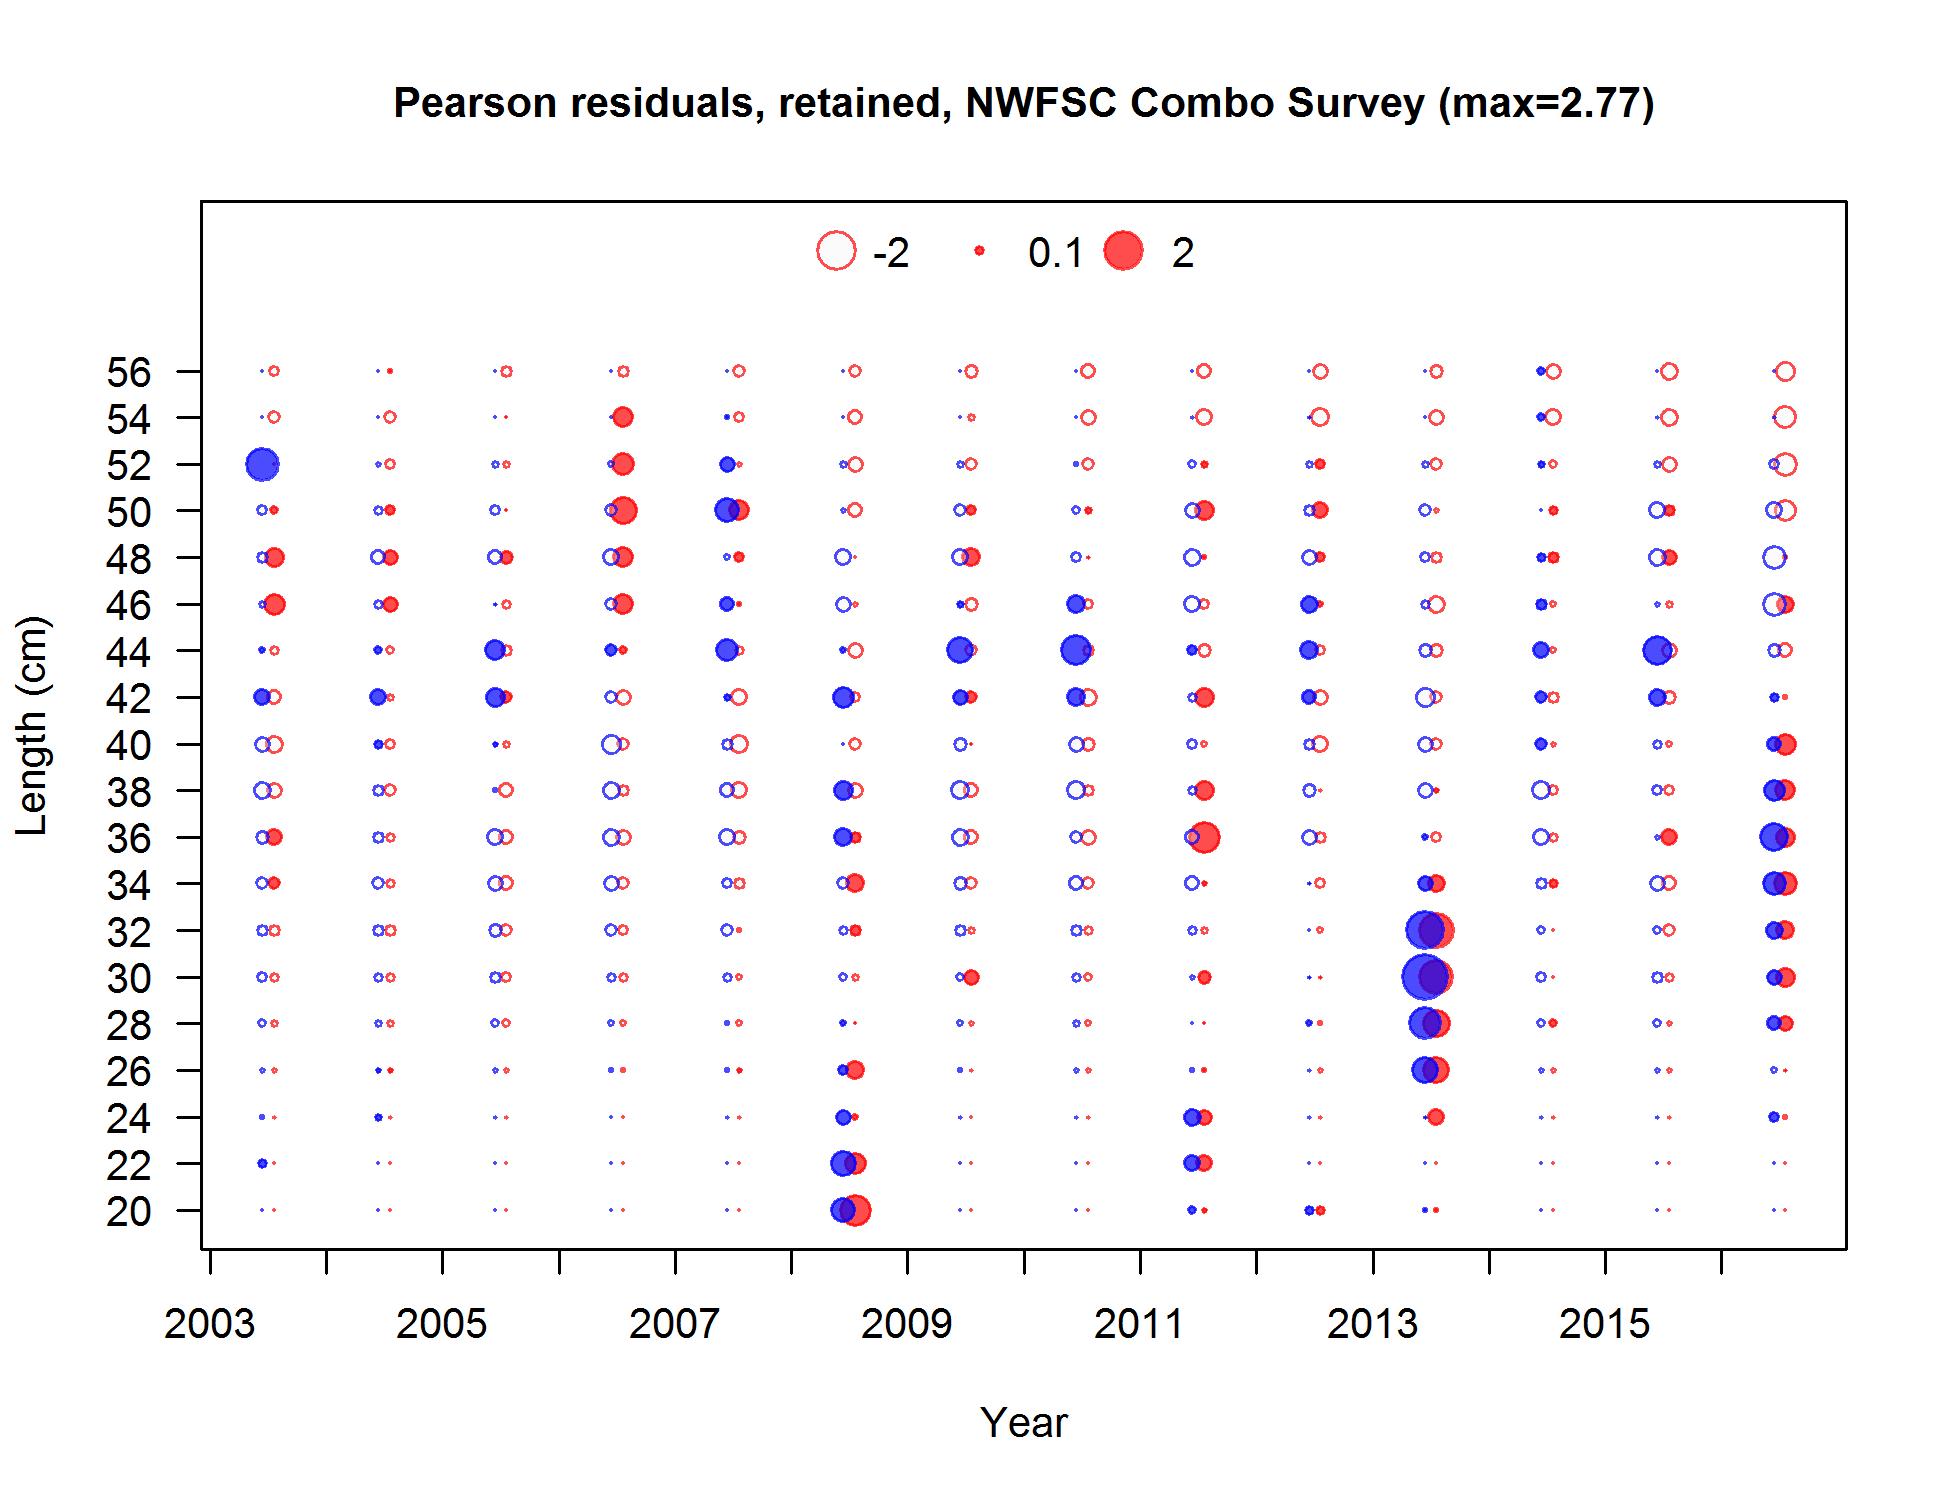
\includegraphics{./r4ss/plots_mod1/comp_lenfit_residsflt6mkt2.png}
\caption{\textbf{Northern model} Pearson residuals, retained, NWFSCcombo
(max=2.68)\\
Closed bubbles are positive residuals (observed \textgreater{} expected)
and open bubbles are negative residuals (observed \textless{} expected).
\label{fig:mod1_27_comp_lenfit_residsflt6mkt2}}
\end{figure}

\begin{figure}[htbp]
\centering
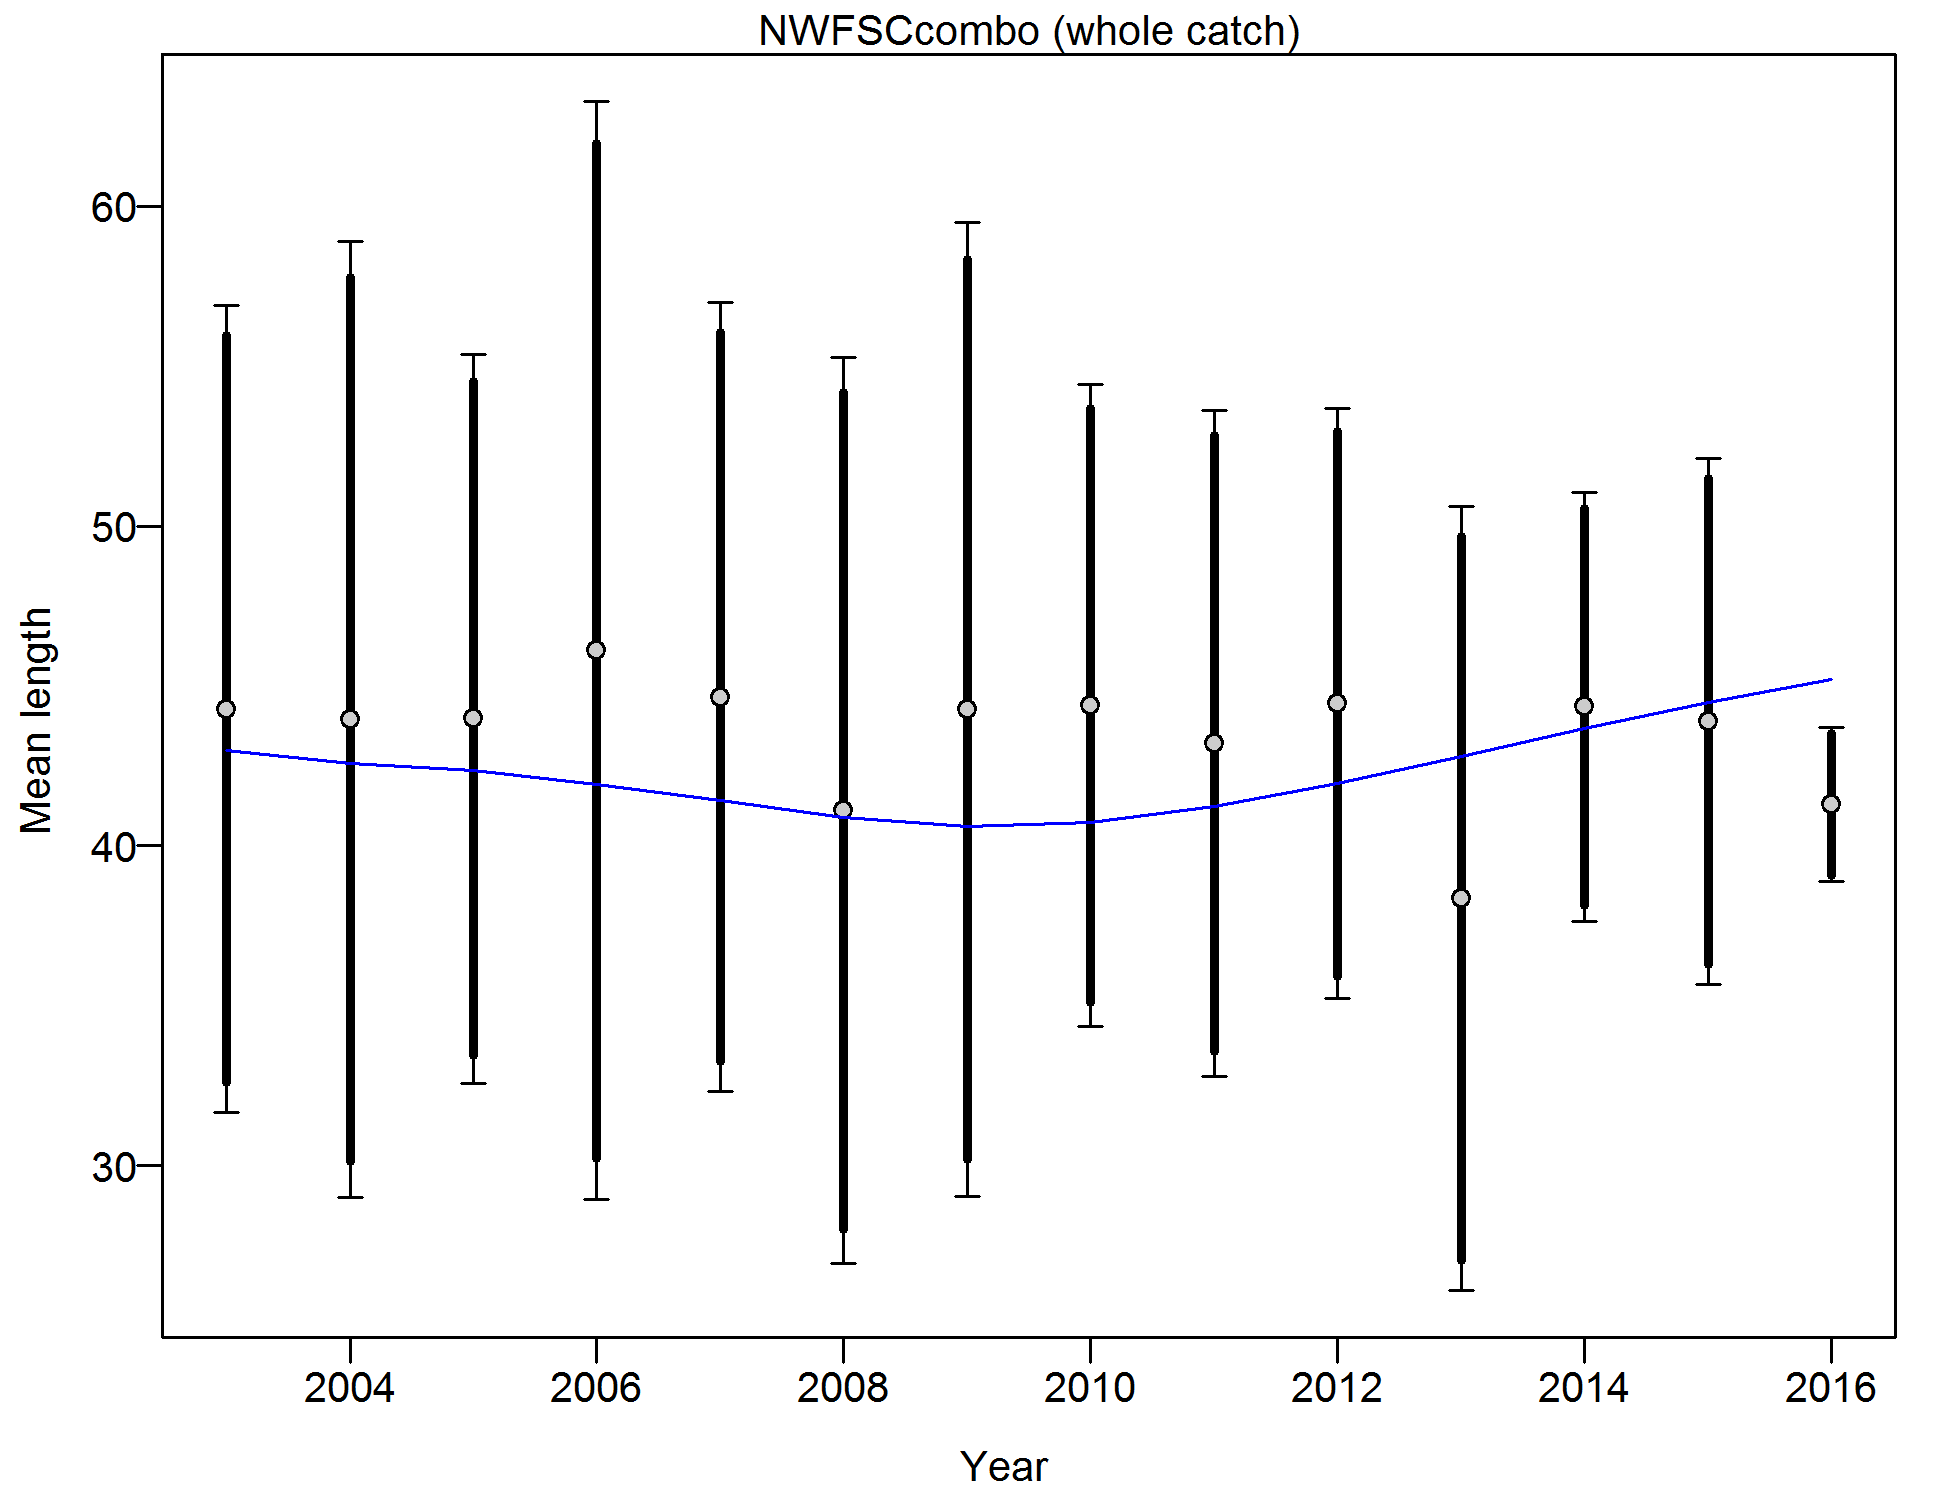
\includegraphics{./r4ss/plots_mod1/comp_lenfit_data_weighting_TA1.8_NWFSCcombo.png}
\caption{\textbf{Northern model} Francis data weighting method TA1.8:
NWFSCcombo Suggested sample size adjustment (with 95\% interval) for len
data from NWFSCcombo: 1.0144 (0.6332\_5.1343) For more info, see
Francis, R.I.C.C. (2011). Data weighting in statistical fisheries stock
assessment models. Can. J. Fish. Aquat. Sci. 68: 1124\_1138.
\label{fig:mod1_29_comp_lenfit_data_weighting_TA1.8_NWFSCcombo}}
\end{figure}

\begin{figure}[htbp]
\centering
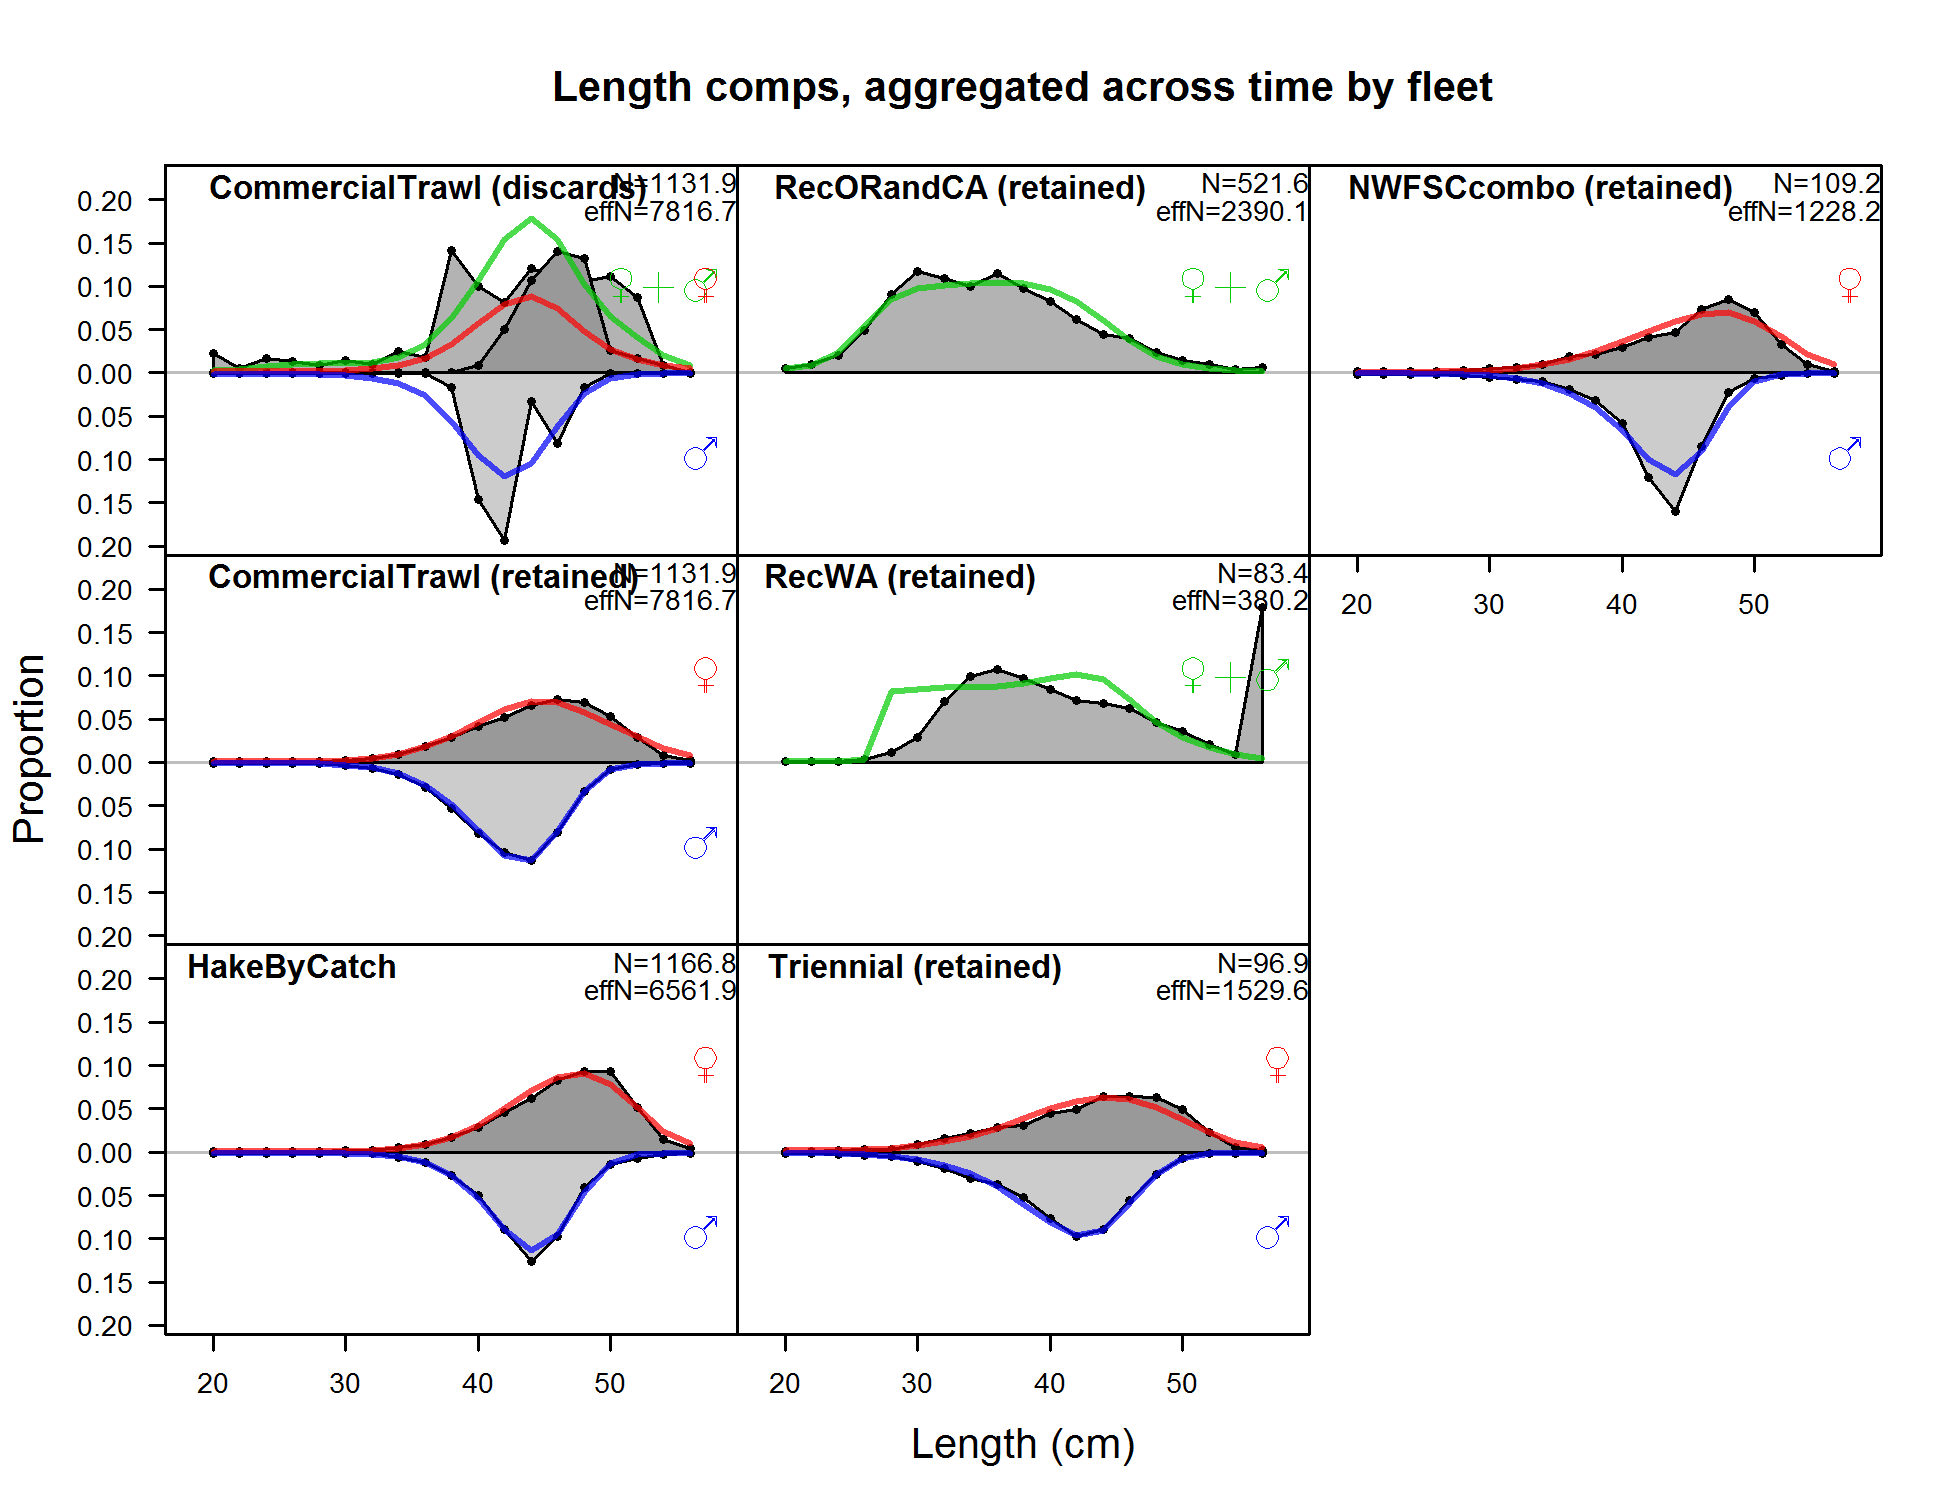
\includegraphics{./r4ss/plots_mod1/comp_lenfit__aggregated_across_time.png}
\caption{\textbf{Northern model} Length comps, aggregated across time by
fleet. Labels `retained' and `discard' indicate discarded or retained
sampled for each fleet. Panels without this designation represent the
whole catch. \label{fig:mod1_30_comp_lenfit__aggregated_across_time}}
\end{figure}

\begin{figure}[htbp]
\centering
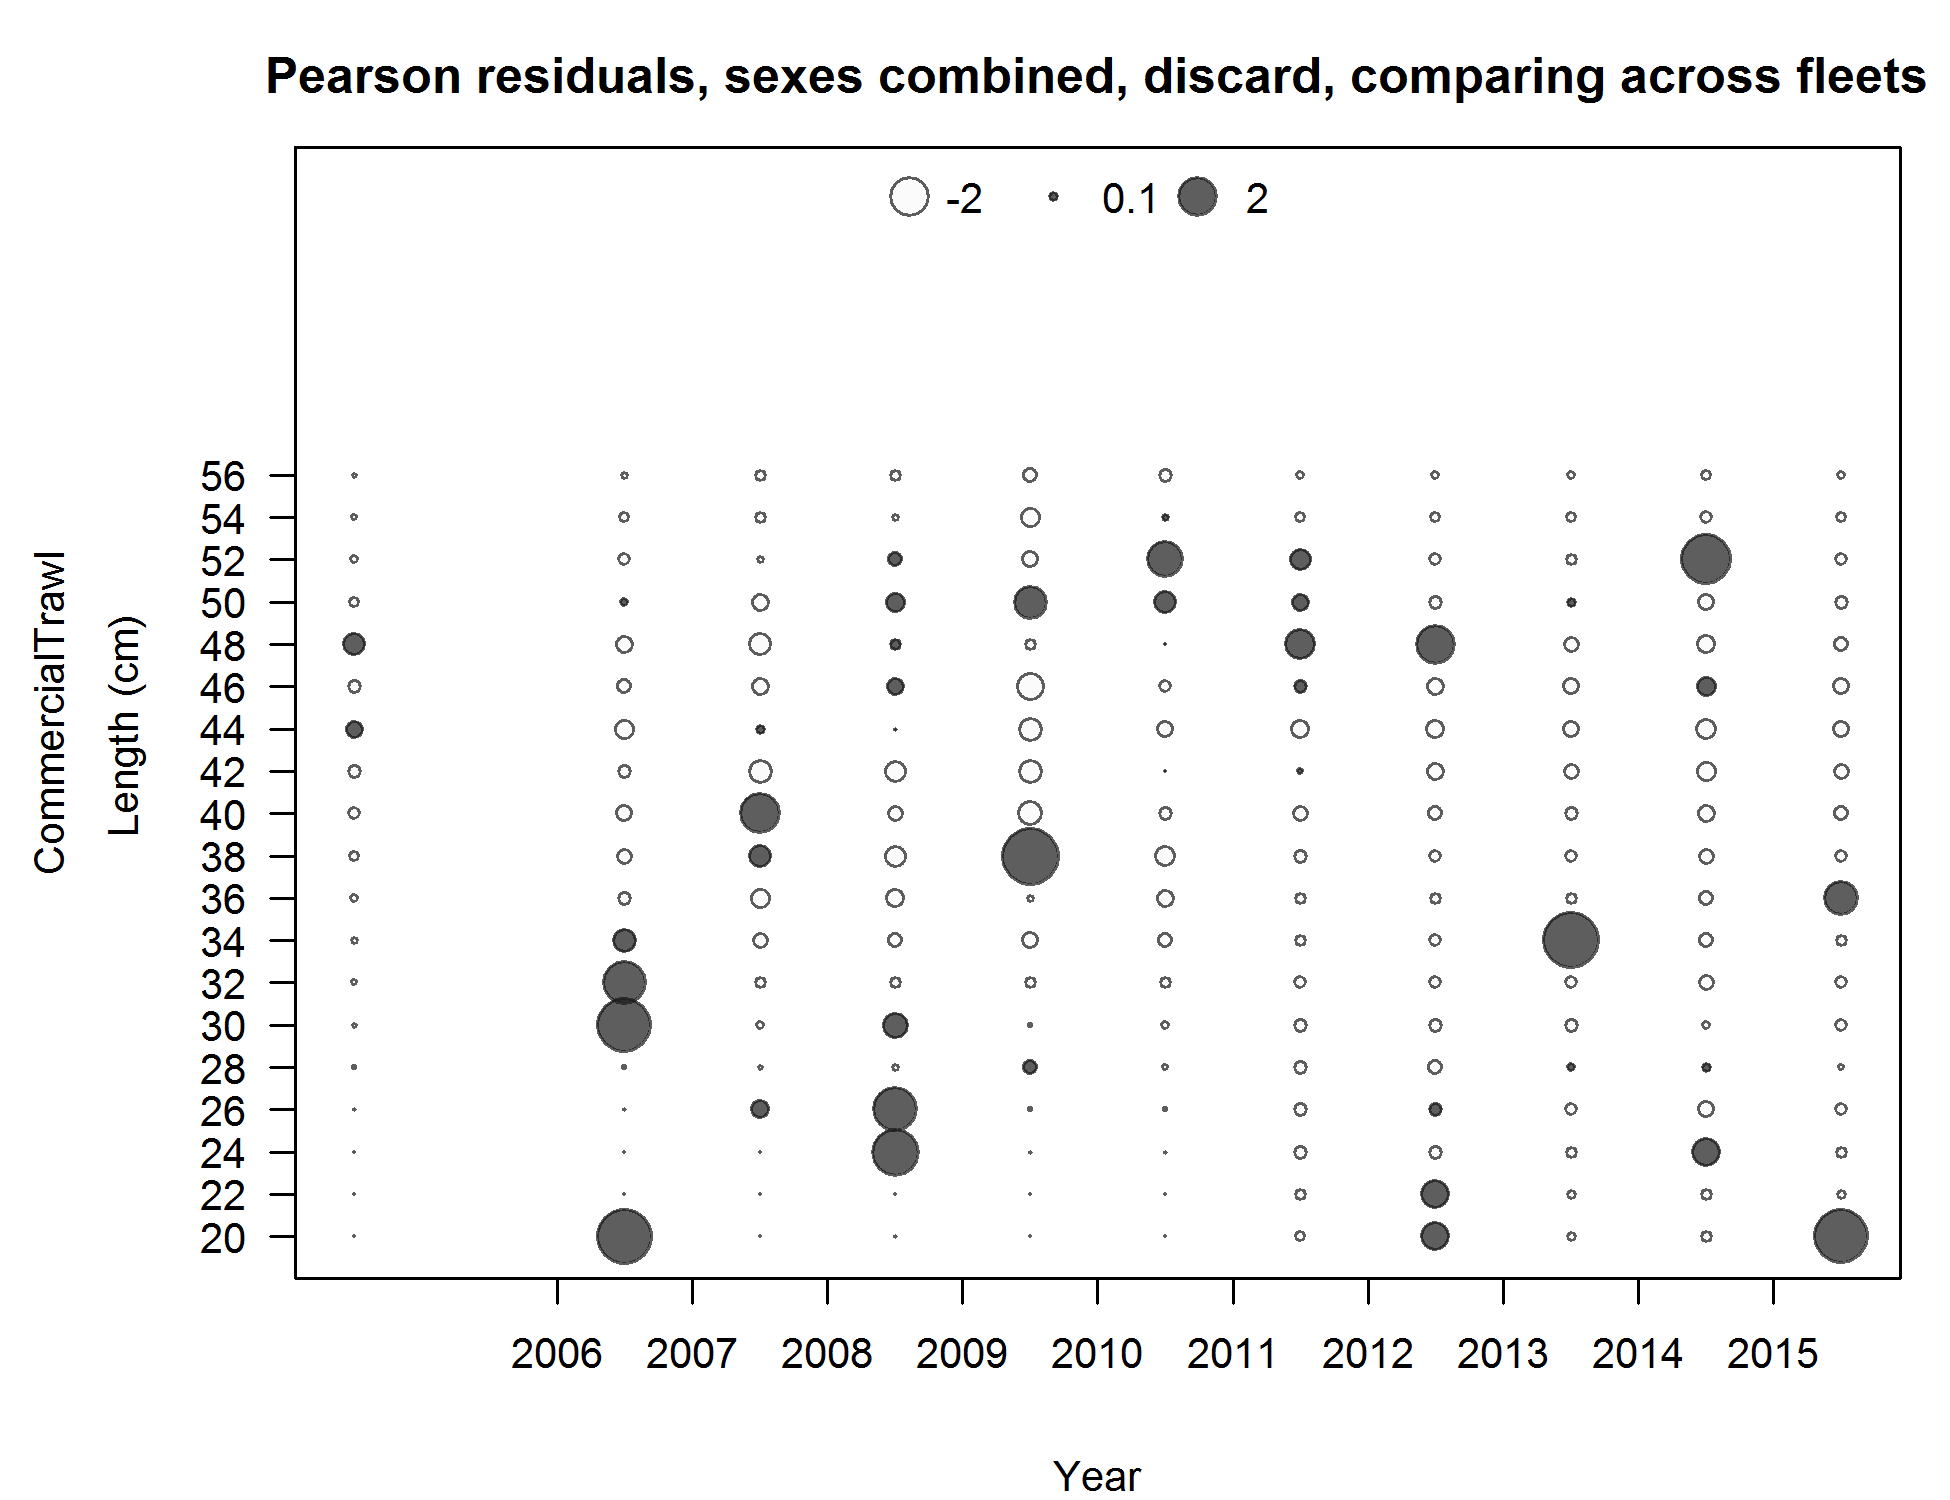
\includegraphics{./r4ss/plots_mod1/comp_lenfit_sex1mkt1_multi-fleet_comparison.png}
\caption{\textbf{Northern model} Note: this plot doesn't seem to be
working right for some models. Pearson residuals, sexes combined,
discard, comparing across fleets\\
Closed bubbles are positive residuals (observed \textgreater{} expected)
and open bubbles are negative residuals (observed \textless{} expected).
\label{fig:mod1_31_comp_lenfit_sex1mkt1_multi-fleet_comparison}}
\end{figure}

\begin{figure}[htbp]
\centering
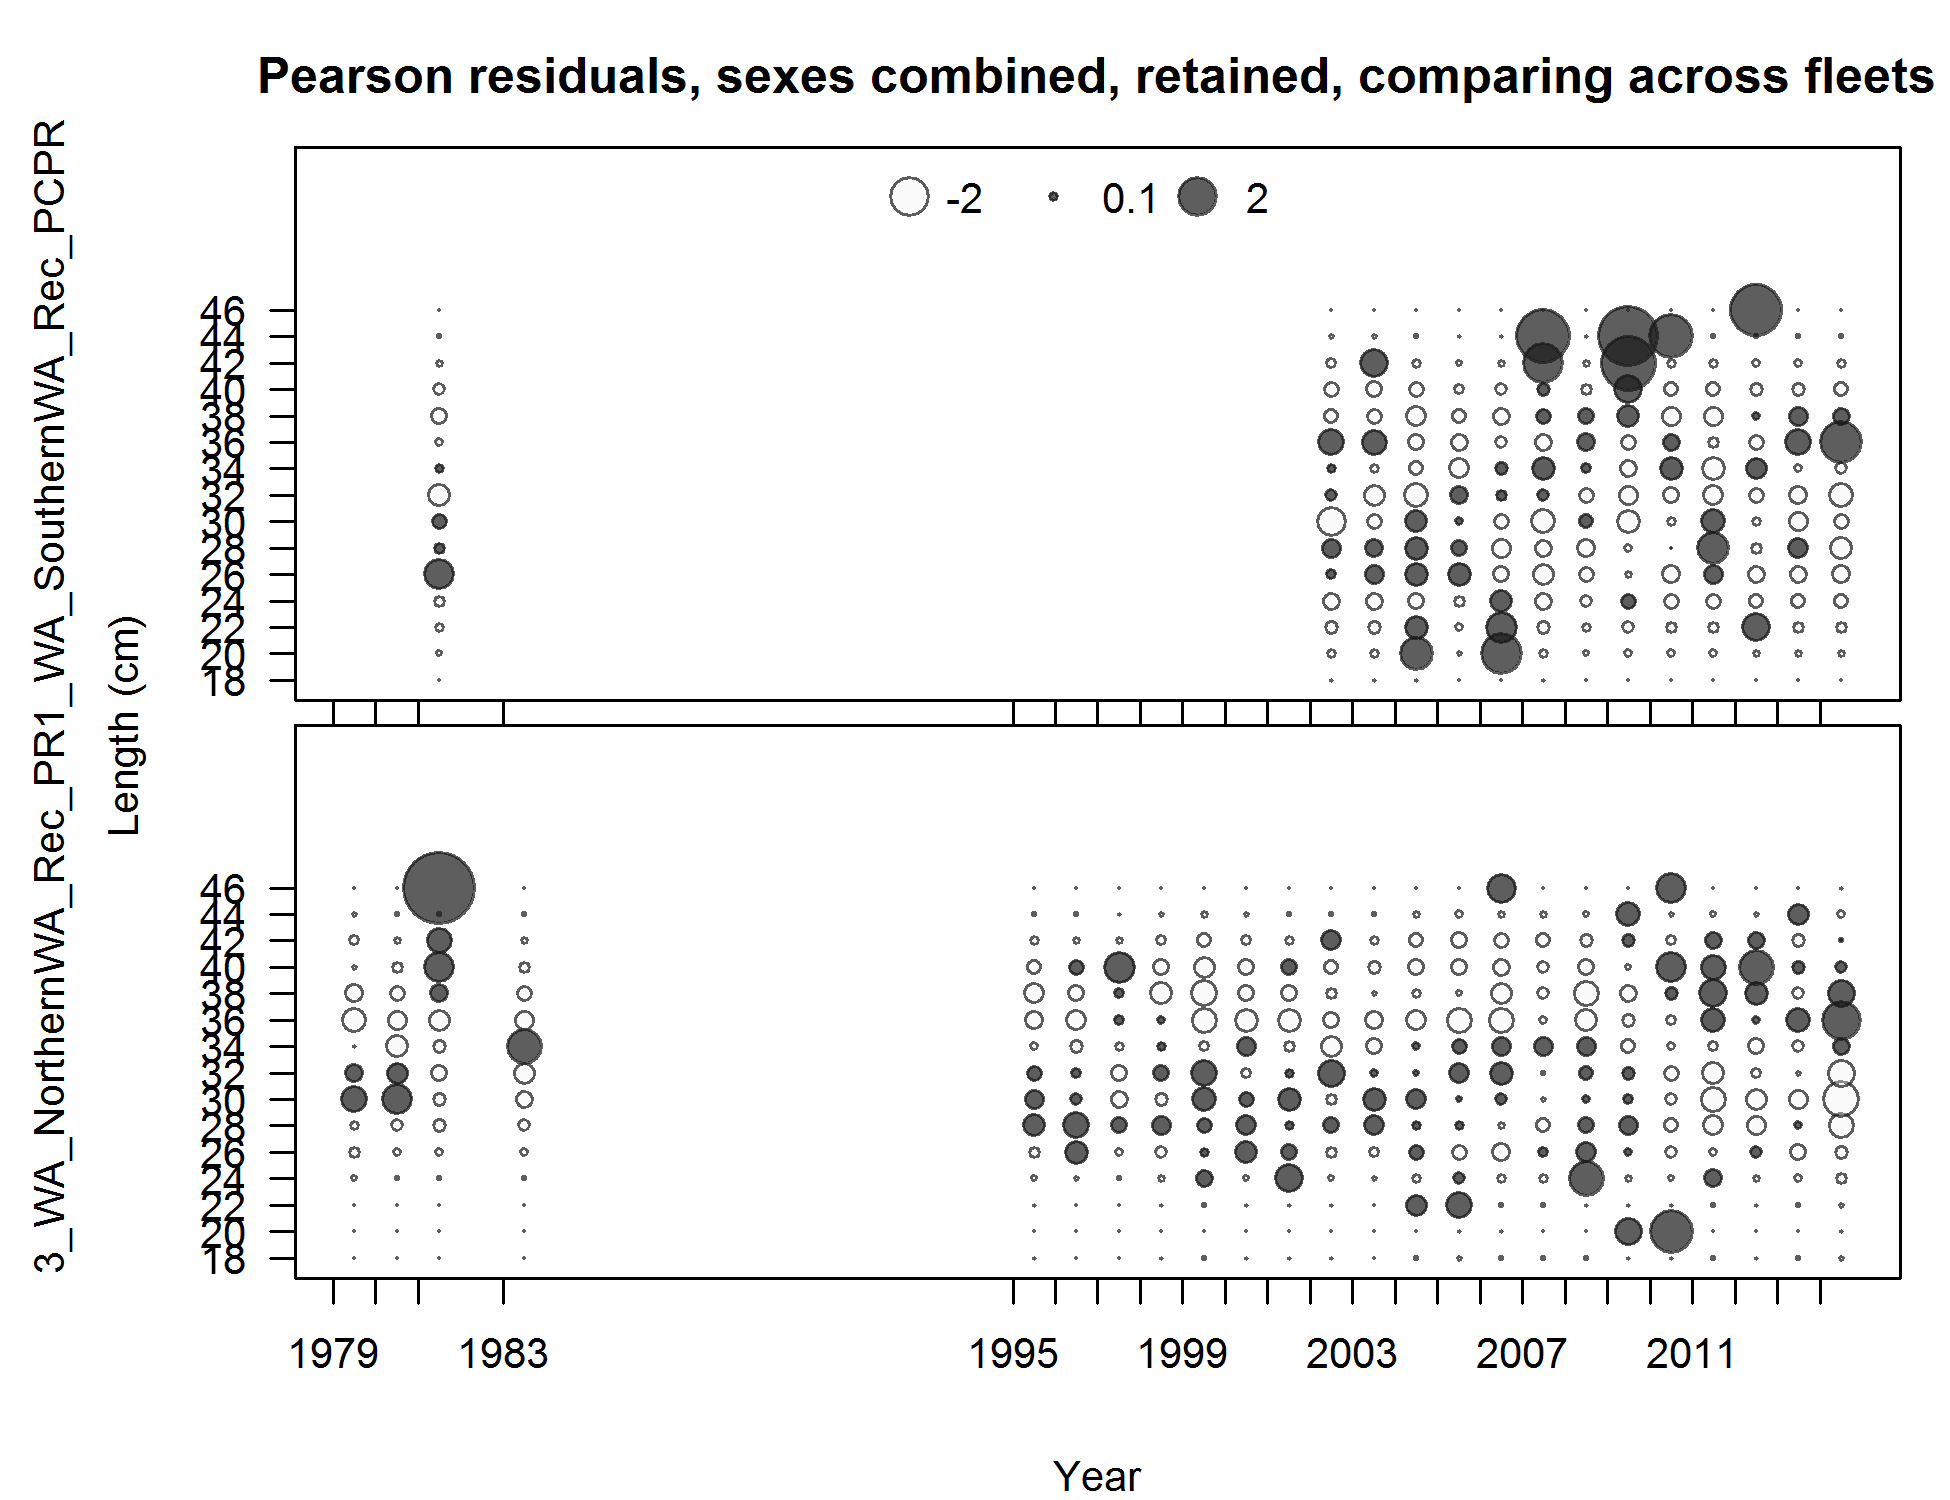
\includegraphics{./r4ss/plots_mod1/comp_lenfit_sex1mkt2_multi-fleet_comparison.png}
\caption{\textbf{Northern model} Note: this plot doesn't seem to be
working right for some models. Pearson residuals, sexes combined,
retained, comparing across fleets\\
Closed bubbles are positive residuals (observed \textgreater{} expected)
and open bubbles are negative residuals (observed \textless{} expected).
\label{fig:mod1_32_comp_lenfit_sex1mkt2_multi-fleet_comparison}}
\end{figure}

\begin{figure}[htbp]
\centering
\includegraphics{./r4ss/plots_mod1/comp_lenfit_sex2mkt2_multi-fleet_comparison.png}
\caption{\textbf{Northern model} Note: this plot doesn't seem to be
working right for some models. Pearson residuals, female, retained,
comparing across fleets\\
Closed bubbles are positive residuals (observed \textgreater{} expected)
and open bubbles are negative residuals (observed \textless{} expected).
\label{fig:mod1_33_comp_lenfit_sex2mkt2_multi-fleet_comparison}}
\end{figure}

\begin{figure}[htbp]
\centering
\includegraphics{./r4ss/plots_mod1/comp_lenfit_sex2mkt1_multi-fleet_comparison.png}
\caption{\textbf{Northern model} Note: this plot doesn't seem to be
working right for some models. Pearson residuals, female, discard,
comparing across fleets\\
Closed bubbles are positive residuals (observed \textgreater{} expected)
and open bubbles are negative residuals (observed \textless{} expected).
\label{fig:mod1_34_comp_lenfit_sex2mkt1_multi-fleet_comparison}}
\end{figure}

\begin{figure}[htbp]
\centering
\includegraphics{./r4ss/plots_mod1/comp_lenfit_sex2mkt0_multi-fleet_comparison.png}
\caption{\textbf{Northern model} Note: this plot doesn't seem to be
working right for some models. Pearson residuals, female, whole catch,
comparing across fleets\\
Closed bubbles are positive residuals (observed \textgreater{} expected)
and open bubbles are negative residuals (observed \textless{} expected).
\label{fig:mod1_35_comp_lenfit_sex2mkt0_multi-fleet_comparison}}
\end{figure}

\begin{figure}[htbp]
\centering
\includegraphics{./r4ss/plots_mod1/comp_lenfit_sex3mkt2_multi-fleet_comparison.png}
\caption{\textbf{Northern model} Note: this plot doesn't seem to be
working right for some models. Pearson residuals, male, retained,
comparing across fleets\\
Closed bubbles are positive residuals (observed \textgreater{} expected)
and open bubbles are negative residuals (observed \textless{} expected).
\label{fig:mod1_36_comp_lenfit_sex3mkt2_multi-fleet_comparison}}
\end{figure}

\begin{figure}[htbp]
\centering
\includegraphics{./r4ss/plots_mod1/comp_lenfit_sex3mkt1_multi-fleet_comparison.png}
\caption{\textbf{Northern model} Note: this plot doesn't seem to be
working right for some models. Pearson residuals, male, discard,
comparing across fleets\\
Closed bubbles are positive residuals (observed \textgreater{} expected)
and open bubbles are negative residuals (observed \textless{} expected).
\label{fig:mod1_37_comp_lenfit_sex3mkt1_multi-fleet_comparison}}
\end{figure}

\begin{figure}[htbp]
\centering
\includegraphics{./r4ss/plots_mod1/comp_lenfit_sex3mkt0_multi-fleet_comparison.png}
\caption{\textbf{Northern model} Note: this plot doesn't seem to be
working right for some models. Pearson residuals, male, whole catch,
comparing across fleets\\
Closed bubbles are positive residuals (observed \textgreater{} expected)
and open bubbles are negative residuals (observed \textless{} expected).
\label{fig:mod1_38_comp_lenfit_sex3mkt0_multi-fleet_comparison}}
\end{figure}

\begin{figure}[htbp]
\centering
\includegraphics{./r4ss/plots_mod1/comp_gstlenfit_flt1mkt2.png}
\caption{\textbf{Northern model} Ghost length comps, retained,
CommercialTrawl \label{fig:mod1_39_comp_gstlenfit_flt1mkt2}}
\end{figure}

\begin{figure}[htbp]
\centering
\includegraphics{./r4ss/plots_mod1/comp_gstlenfit_residsflt1mkt2.png}
\caption{\textbf{Northern model} Pearson residuals, retained,
CommercialTrawl (max=NA)\\
Closed bubbles are positive residuals (observed \textgreater{} expected)
and open bubbles are negative residuals (observed \textless{} expected).
\label{fig:mod1_40_comp_gstlenfit_residsflt1mkt2}}
\end{figure}

\FloatBarrier

\subsubsection{Fits to length compositions for Southern
model}\label{fits-to-length-compositions-for-southern-model}

\begin{figure}[htbp]
\centering
\includegraphics{./r4ss/plots_mod2/comp_lenfit_flt1mkt2.png}
\caption{\textbf{Southern model} Length comps, retained,
RecreationalCatch \label{fig:mod2_1_comp_lenfit_flt1mkt2}}
\end{figure}

\begin{figure}[htbp]
\centering
\includegraphics{./r4ss/plots_mod2/comp_lenfit_residsflt1mkt2.png}
\caption{\textbf{Southern model} Pearson residuals, retained,
RecreationalCatch (max=4.4)\\
Closed bubbles are positive residuals (observed \textgreater{} expected)
and open bubbles are negative residuals (observed \textless{} expected).
\label{fig:mod2_2_comp_lenfit_residsflt1mkt2}}
\end{figure}

\begin{figure}[htbp]
\centering
\includegraphics{./r4ss/plots_mod2/comp_lenfit_data_weighting_TA1.8_RecreationalCatch.png}
\caption{\textbf{Southern model} Francis data weighting method TA1.8:
RecreationalCatch Suggested sample size adjustment (with 95\% interval)
for len data from RecreationalCatch: 0.9238 (0.6097\_1.7877) For more
info, see Francis, R.I.C.C. (2011). Data weighting in statistical
fisheries stock assessment models. Can. J. Fish. Aquat. Sci. 68:
1124\_1138.
\label{fig:mod2_4_comp_lenfit_data_weighting_TA1.8_RecreationalCatch}}
\end{figure}

\begin{figure}[htbp]
\centering
\includegraphics{./r4ss/plots_mod2/comp_lenfit_flt2mkt2.png}
\caption{\textbf{Southern model} Length comps, retained, CommercialCatch
\label{fig:mod2_5_comp_lenfit_flt2mkt2}}
\end{figure}

\begin{figure}[htbp]
\centering
\includegraphics{./r4ss/plots_mod2/comp_lenfit_residsflt2mkt2.png}
\caption{\textbf{Southern model} Pearson residuals, retained,
CommercialCatch (max=5.72)\\
Closed bubbles are positive residuals (observed \textgreater{} expected)
and open bubbles are negative residuals (observed \textless{} expected).
\label{fig:mod2_6_comp_lenfit_residsflt2mkt2}}
\end{figure}

\begin{figure}[htbp]
\centering
\includegraphics{./r4ss/plots_mod2/comp_lenfit_data_weighting_TA1.8_CommercialCatch.png}
\caption{\textbf{Southern model} Francis data weighting method TA1.8:
CommercialCatch Suggested sample size adjustment (with 95\% interval)
for len data from CommercialCatch: 0.9835 (0.6829\_1.8164) For more
info, see Francis, R.I.C.C. (2011). Data weighting in statistical
fisheries stock assessment models. Can. J. Fish. Aquat. Sci. 68:
1124\_1138.
\label{fig:mod2_8_comp_lenfit_data_weighting_TA1.8_CommercialCatch}}
\end{figure}

\begin{figure}[htbp]
\centering
\includegraphics{./r4ss/plots_mod2/comp_lenfit_flt3mkt2.png}
\caption{\textbf{Southern model} Length comps, retained, OnboardSurvey
\label{fig:mod2_9_comp_lenfit_flt3mkt2}}
\end{figure}

\begin{figure}[htbp]
\centering
\includegraphics{./r4ss/plots_mod2/comp_lenfit_residsflt3mkt2.png}
\caption{\textbf{Southern model} Pearson residuals, retained,
OnboardSurvey (max=5.23)\\
Closed bubbles are positive residuals (observed \textgreater{} expected)
and open bubbles are negative residuals (observed \textless{} expected).
\label{fig:mod2_10_comp_lenfit_residsflt3mkt2}}
\end{figure}

\begin{figure}[htbp]
\centering
\includegraphics{./r4ss/plots_mod2/comp_lenfit_data_weighting_TA1.8_OnboardSurvey.png}
\caption{\textbf{Southern model} Francis data weighting method TA1.8:
OnboardSurvey Suggested sample size adjustment (with 95\% interval) for
len data from OnboardSurvey: 0.7823 (0.5494\_1.4862) For more info, see
Francis, R.I.C.C. (2011). Data weighting in statistical fisheries stock
assessment models. Can. J. Fish. Aquat. Sci. 68: 1124\_1138.
\label{fig:mod2_12_comp_lenfit_data_weighting_TA1.8_OnboardSurvey}}
\end{figure}

\begin{figure}[htbp]
\centering
\includegraphics{./r4ss/plots_mod2/comp_lenfit_flt4mkt0.png}
\caption{\textbf{Southern model} Length comps, whole catch,
HookAndLineSurvey \label{fig:mod2_13_comp_lenfit_flt4mkt0}}
\end{figure}

\begin{figure}[htbp]
\centering
\includegraphics{./r4ss/plots_mod2/comp_lenfit_residsflt4mkt0.png}
\caption{\textbf{Southern model} Pearson residuals, whole catch,
HookAndLineSurvey (max=2.92)\\
Closed bubbles are positive residuals (observed \textgreater{} expected)
and open bubbles are negative residuals (observed \textless{} expected).
\label{fig:mod2_14_comp_lenfit_residsflt4mkt0}}
\end{figure}

\begin{figure}[htbp]
\centering
\includegraphics{./r4ss/plots_mod2/comp_lenfit_data_weighting_TA1.8_HookAndLineSurvey.png}
\caption{\textbf{Southern model} Francis data weighting method TA1.8:
HookAndLineSurvey Suggested sample size adjustment (with 95\% interval)
for len data from HookAndLineSurvey: 1.0633 (0.74\_2.6995) For more
info, see Francis, R.I.C.C. (2011). Data weighting in statistical
fisheries stock assessment models. Can. J. Fish. Aquat. Sci. 68:
1124\_1138.
\label{fig:mod2_16_comp_lenfit_data_weighting_TA1.8_HookAndLineSurvey}}
\end{figure}

\begin{figure}[htbp]
\centering
\includegraphics{./r4ss/plots_mod2/comp_lenfit_flt5mkt2.png}
\caption{\textbf{Southern model} Length comps, retained, RecStudy
\label{fig:mod2_17_comp_lenfit_flt5mkt2}}
\end{figure}

\begin{figure}[htbp]
\centering
\includegraphics{./r4ss/plots_mod2/comp_lenfit_residsflt5mkt2.png}
\caption{\textbf{Southern model} Pearson residuals, retained, RecStudy
(max=2.16)\\
Closed bubbles are positive residuals (observed \textgreater{} expected)
and open bubbles are negative residuals (observed \textless{} expected).
\label{fig:mod2_18_comp_lenfit_residsflt5mkt2}}
\end{figure}

\begin{figure}[htbp]
\centering
\includegraphics{./r4ss/plots_mod2/comp_lenfit_data_weighting_TA1.8_RecStudy.png}
\caption{\textbf{Southern model} Francis data weighting method TA1.8:
RecStudy Suggested sample size adjustment (with 95\% interval) for len
data from RecStudy: 1.0664 (0.5599\_16.048) For more info, see Francis,
R.I.C.C. (2011). Data weighting in statistical fisheries stock
assessment models. Can. J. Fish. Aquat. Sci. 68: 1124\_1138.
\label{fig:mod2_20_comp_lenfit_data_weighting_TA1.8_RecStudy}}
\end{figure}

\begin{figure}[htbp]
\centering
\includegraphics{./r4ss/plots_mod2/comp_lenfit__aggregated_across_time.png}
\caption{\textbf{Southern model} Length comps, aggregated across time by
fleet. Labels `retained' and `discard' indicate discarded or retained
sampled for each fleet. Panels without this designation represent the
whole catch. \label{fig:mod2_21_comp_lenfit__aggregated_across_time}}
\end{figure}

\begin{figure}[htbp]
\centering
\includegraphics{./r4ss/plots_mod2/comp_lenfit_sex1mkt2_multi-fleet_comparison.png}
\caption{\textbf{Southern model} Note: this plot doesn't seem to be
working right for some models. Pearson residuals, sexes combined,
retained, comparing across fleets\\
Closed bubbles are positive residuals (observed \textgreater{} expected)
and open bubbles are negative residuals (observed \textless{} expected).
\label{fig:mod2_22_comp_lenfit_sex1mkt2_multi-fleet_comparison}}
\end{figure}

\begin{figure}[htbp]
\centering
\includegraphics{./r4ss/plots_mod2/comp_lenfit_sex2mkt0_multi-fleet_comparison.png}
\caption{\textbf{Southern model} Note: this plot doesn't seem to be
working right for some models. Pearson residuals, female, whole catch,
comparing across fleets\\
Closed bubbles are positive residuals (observed \textgreater{} expected)
and open bubbles are negative residuals (observed \textless{} expected).
\label{fig:mod2_23_comp_lenfit_sex2mkt0_multi-fleet_comparison}}
\end{figure}

\begin{figure}[htbp]
\centering
\includegraphics{./r4ss/plots_mod2/comp_lenfit_sex3mkt0_multi-fleet_comparison.png}
\caption{\textbf{Southern model} Note: this plot doesn't seem to be
working right for some models. Pearson residuals, male, whole catch,
comparing across fleets\\
Closed bubbles are positive residuals (observed \textgreater{} expected)
and open bubbles are negative residuals (observed \textless{} expected).
\label{fig:mod2_24_comp_lenfit_sex3mkt0_multi-fleet_comparison}}
\end{figure}

\FloatBarrier

\subsubsection{Fits to age compositions for Northern
model}\label{fits-to-age-compositions-for-northern-model}

\begin{figure}[htbp]
\centering
\includegraphics{./r4ss/plots_mod1/comp_agefit_flt1mkt2_page1.png}
\caption{\textbf{Northern model} Age comps, retained, CommercialTrawl
(plot 1 of 2) \label{fig:mod1_1_comp_agefit_flt1mkt2_page1}}
\end{figure}

\includegraphics{./r4ss/plots_mod1/comp_agefit_flt1mkt2_page2.png}

\begin{center} 

            Figure continued from previous page 

            \end{center}

\includegraphics{./r4ss/plots_mod1/comp_agefit_residsflt1mkt2_page2.png}

\begin{center} 

            Figure continued from previous page 

            \end{center}

\begin{figure}[htbp]
\centering
\includegraphics{./r4ss/plots_mod1/comp_agefit_data_weighting_TA1.8_CommercialTrawl.png}
\caption{\textbf{Northern model} Francis data weighting method TA1.8:
CommercialTrawl Suggested sample size adjustment (with 95\% interval)
for age data from CommercialTrawl: 1.1663 (0.7554\_2.1133) For more
info, see Francis, R.I.C.C. (2011). Data weighting in statistical
fisheries stock assessment models. Can. J. Fish. Aquat. Sci. 68:
1124\_1138.
\label{fig:mod1_5_comp_agefit_data_weighting_TA1.8_CommercialTrawl}}
\end{figure}

\begin{figure}[htbp]
\centering
\includegraphics{./r4ss/plots_mod1/comp_agefit_flt4mkt2.png}
\caption{\textbf{Northern model} Age comps, retained, RecWA
\label{fig:mod1_6_comp_agefit_flt4mkt2}}
\end{figure}

\begin{figure}[htbp]
\centering
\includegraphics{./r4ss/plots_mod1/comp_agefit_residsflt4mkt2.png}
\caption{\textbf{Northern model} Pearson residuals, retained, RecWA
(max=2.68)\\
Closed bubbles are positive residuals (observed \textgreater{} expected)
and open bubbles are negative residuals (observed \textless{} expected).
\label{fig:mod1_7_comp_agefit_residsflt4mkt2}}
\end{figure}

\begin{figure}[htbp]
\centering
\includegraphics{./r4ss/plots_mod1/comp_agefit_data_weighting_TA1.8_RecWA.png}
\caption{\textbf{Northern model} Francis data weighting method TA1.8:
RecWA Suggested sample size adjustment (with 95\% interval) for age data
from RecWA: 1.0396 (0.6753\_3.901) For more info, see Francis, R.I.C.C.
(2011). Data weighting in statistical fisheries stock assessment models.
Can. J. Fish. Aquat. Sci. 68: 1124\_1138.
\label{fig:mod1_9_comp_agefit_data_weighting_TA1.8_RecWA}}
\end{figure}

\begin{figure}[htbp]
\centering
\includegraphics{./r4ss/plots_mod1/comp_agefit_flt5mkt2.png}
\caption{\textbf{Northern model} Age comps, retained, Triennial
\label{fig:mod1_10_comp_agefit_flt5mkt2}}
\end{figure}

\begin{figure}[htbp]
\centering
\includegraphics{./r4ss/plots_mod1/comp_agefit_residsflt5mkt2.png}
\caption{\textbf{Northern model} Pearson residuals, retained, Triennial
(max=1.24)\\
Closed bubbles are positive residuals (observed \textgreater{} expected)
and open bubbles are negative residuals (observed \textless{} expected).
\label{fig:mod1_11_comp_agefit_residsflt5mkt2}}
\end{figure}

\begin{figure}[htbp]
\centering
\includegraphics{./r4ss/plots_mod1/comp_agefit_data_weighting_TA1.8_Triennial.png}
\caption{\textbf{Northern model} Francis data weighting method TA1.8:
Triennial Suggested sample size adjustment (with 95\% interval) for age
data from Triennial: 1.0944 (0.6476\_3.7348) For more info, see Francis,
R.I.C.C. (2011). Data weighting in statistical fisheries stock
assessment models. Can. J. Fish. Aquat. Sci. 68: 1124\_1138.
\label{fig:mod1_13_comp_agefit_data_weighting_TA1.8_Triennial}}
\end{figure}

\begin{figure}[htbp]
\centering
\includegraphics{./r4ss/plots_mod1/comp_agefit__aggregated_across_time.png}
\caption{\textbf{Northern model} Age comps, aggregated across time by
fleet. Labels `retained' and `discard' indicate discarded or retained
sampled for each fleet. Panels without this designation represent the
whole catch. \label{fig:mod1_14_comp_agefit__aggregated_across_time}}
\end{figure}

\begin{figure}[htbp]
\centering
\includegraphics{./r4ss/plots_mod1/comp_agefit_sex2mkt2_multi-fleet_comparison.png}
\caption{\textbf{Northern model} Note: this plot doesn't seem to be
working right for some models. Pearson residuals, female, retained,
comparing across fleets\\
Closed bubbles are positive residuals (observed \textgreater{} expected)
and open bubbles are negative residuals (observed \textless{} expected).
\label{fig:mod1_15_comp_agefit_sex2mkt2_multi-fleet_comparison}}
\end{figure}

\begin{figure}[htbp]
\centering
\includegraphics{./r4ss/plots_mod1/comp_agefit_sex3mkt2_multi-fleet_comparison.png}
\caption{\textbf{Northern model} Note: this plot doesn't seem to be
working right for some models. Pearson residuals, male, retained,
comparing across fleets\\
Closed bubbles are positive residuals (observed \textgreater{} expected)
and open bubbles are negative residuals (observed \textless{} expected).
\label{fig:mod1_16_comp_agefit_sex3mkt2_multi-fleet_comparison}}
\end{figure}

\begin{figure}[htbp]
\centering
\includegraphics{./r4ss/plots_mod1/comp_gstagefit_flt6mkt2.png}
\caption{\textbf{Northern model} Ghost age comps, retained, NWFSCcombo
\label{fig:mod1_17_comp_gstagefit_flt6mkt2}}
\end{figure}

\begin{figure}[htbp]
\centering
\includegraphics{./r4ss/plots_mod1/comp_gstagefit_residsflt6mkt2.png}
\caption{\textbf{Northern model} Pearson residuals, retained, NWFSCcombo
(max=NA)\\
Closed bubbles are positive residuals (observed \textgreater{} expected)
and open bubbles are negative residuals (observed \textless{} expected).
\label{fig:mod1_18_comp_gstagefit_residsflt6mkt2}}
\end{figure}

\FloatBarrier

\newpage

\subsubsection{Fits to conditional-age-at-length compositions for
Northern
model}\label{fits-to-conditional-age-at-length-compositions-for-northern-model}

\begin{figure}[htbp]
\centering
\includegraphics{./r4ss/plots_mod1/comp_condAALfit_residsflt6mkt2_page1.png}
\caption{\textbf{Northern model} Pearson residuals, retained, NWFSCcombo
(max=8.29) (plot 1 of 2)
\label{fig:mod1_1_comp_condAALfit_residsflt6mkt2_page1}}
\end{figure}

\includegraphics{./r4ss/plots_mod1/comp_condAALfit_residsflt6mkt2_page2.png}

\begin{center} 

            Figure continued from previous page 

            \end{center}

\begin{figure}[htbp]
\centering
\includegraphics{./r4ss/plots_mod1/comp_condAALfit_data_weighting_TA1.8_condAgeNWFSCcombo.png}
\caption{\textbf{Northern model} Francis data weighting method TA1.8 for
conditional age \url{data:NWFSCcombo} Suggested sample size
adjustment(with 95\% interval) forconditional age\_at\_length data from
NWFSCcombo: 1.0265 (0.6887\_2.3764) For more info, see Francis, R.I.C.C.
(2011). Data weighting in statistical fisheries stock assessment models.
Can. J. Fish. Aquat. Sci. 68: 1124\_1138.
\label{fig:mod1_3_comp_condAALfit_data_weighting_TA1.8_condAgeNWFSCcombo}}
\end{figure}

\begin{figure}[htbp]
\centering
\includegraphics{./r4ss/plots_mod1/comp_condAALfit_Andre_plotsflt6mkt2_page1.png}
\caption{\textbf{Northern model} Conditional AAL plot, retained,
NWFSCcombo (plot 1 of 5) These plots show mean age and std. dev. in
conditional AAL. Left plots are mean AAL by size\_class (obs. and pred.)
with 90\% CIs based on adding 1.64 SE of mean to the data. Right plots
in each pair are SE of mean AAL (obs. and pred.) with 90\% CIs based on
the chi\_square distribution.
\label{fig:mod1_4_comp_condAALfit_Andre_plotsflt6mkt2_page1}}
\end{figure}

\includegraphics{./r4ss/plots_mod1/comp_condAALfit_Andre_plotsflt6mkt2_page2.png}

\begin{center} 

            Figure continued from previous page 

            \end{center}

\includegraphics{./r4ss/plots_mod1/comp_condAALfit_Andre_plotsflt6mkt2_page3.png}

\begin{center} 

            Figure continued from previous page 

            \end{center}

\includegraphics{./r4ss/plots_mod1/comp_condAALfit_Andre_plotsflt6mkt2_page4.png}

\begin{center} 

            Figure continued from previous page 

            \end{center}

\includegraphics{./r4ss/plots_mod1/comp_condAALfit_Andre_plotsflt6mkt2_page5.png}

\begin{center} 

            Figure continued from previous page 

            \end{center}

\FloatBarrier

\newpage

\subsubsection{Fits to age compositions for Southern
model}\label{fits-to-age-compositions-for-southern-model}

\begin{figure}[htbp]
\centering
\includegraphics{./r4ss/plots_mod2/comp_agefit_flt1mkt2.png}
\caption{\textbf{Southern model} Age comps, retained, RecreationalCatch
\label{fig:mod2_1_comp_agefit_flt1mkt2}}
\end{figure}

\begin{figure}[htbp]
\centering
\includegraphics{./r4ss/plots_mod2/comp_agefit_residsflt1mkt2.png}
\caption{\textbf{Southern model} Pearson residuals, retained,
RecreationalCatch (max=1.36)\\
Closed bubbles are positive residuals (observed \textgreater{} expected)
and open bubbles are negative residuals (observed \textless{} expected).
\label{fig:mod2_2_comp_agefit_residsflt1mkt2}}
\end{figure}

\begin{figure}[htbp]
\centering
\includegraphics{./r4ss/plots_mod2/comp_agefit_data_weighting_TA1.8_RecreationalCatch.png}
\caption{\textbf{Southern model} Francis data weighting method TA1.8:
RecreationalCatch Suggested sample size adjustment (with 95\% interval)
for age data from RecreationalCatch: 0.9648 (0.5135\_28.2193) For more
info, see Francis, R.I.C.C. (2011). Data weighting in statistical
fisheries stock assessment models. Can. J. Fish. Aquat. Sci. 68:
1124\_1138.
\label{fig:mod2_4_comp_agefit_data_weighting_TA1.8_RecreationalCatch}}
\end{figure}

\begin{figure}[htbp]
\centering
\includegraphics{./r4ss/plots_mod2/comp_agefit_flt4mkt0.png}
\caption{\textbf{Southern model} Age comps, whole catch,
HookAndLineSurvey \label{fig:mod2_5_comp_agefit_flt4mkt0}}
\end{figure}

\begin{figure}[htbp]
\centering
\includegraphics{./r4ss/plots_mod2/comp_agefit_residsflt4mkt0.png}
\caption{\textbf{Southern model} Pearson residuals, whole catch,
HookAndLineSurvey (max=4.02)\\
Closed bubbles are positive residuals (observed \textgreater{} expected)
and open bubbles are negative residuals (observed \textless{} expected).
\label{fig:mod2_6_comp_agefit_residsflt4mkt0}}
\end{figure}

\begin{figure}[htbp]
\centering
\includegraphics{./r4ss/plots_mod2/comp_agefit_data_weighting_TA1.8_HookAndLineSurvey.png}
\caption{\textbf{Southern model} Francis data weighting method TA1.8:
HookAndLineSurvey Too few points to calculate adjustments For more info,
see Francis, R.I.C.C. (2011). Data weighting in statistical fisheries
stock assessment models. Can. J. Fish. Aquat. Sci. 68: 1124\_1138.
\label{fig:mod2_8_comp_agefit_data_weighting_TA1.8_HookAndLineSurvey}}
\end{figure}

\begin{figure}[htbp]
\centering
\includegraphics{./r4ss/plots_mod2/comp_agefit__aggregated_across_time.png}
\caption{\textbf{Southern model} Age comps, aggregated across time by
fleet. Labels `retained' and `discard' indicate discarded or retained
sampled for each fleet. Panels without this designation represent the
whole catch. \label{fig:mod2_9_comp_agefit__aggregated_across_time}}
\end{figure}

\begin{figure}[htbp]
\centering
\includegraphics{./r4ss/plots_mod2/comp_agefit_sex2mkt2_multi-fleet_comparison.png}
\caption{\textbf{Southern model} Note: this plot doesn't seem to be
working right for some models. Pearson residuals, female, retained,
comparing across fleets\\
Closed bubbles are positive residuals (observed \textgreater{} expected)
and open bubbles are negative residuals (observed \textless{} expected).
\label{fig:mod2_10_comp_agefit_sex2mkt2_multi-fleet_comparison}}
\end{figure}

\begin{figure}[htbp]
\centering
\includegraphics{./r4ss/plots_mod2/comp_agefit_sex2mkt0_multi-fleet_comparison.png}
\caption{\textbf{Southern model} Note: this plot doesn't seem to be
working right for some models. Pearson residuals, female, whole catch,
comparing across fleets\\
Closed bubbles are positive residuals (observed \textgreater{} expected)
and open bubbles are negative residuals (observed \textless{} expected).
\label{fig:mod2_11_comp_agefit_sex2mkt0_multi-fleet_comparison}}
\end{figure}

\begin{figure}[htbp]
\centering
\includegraphics{./r4ss/plots_mod2/comp_agefit_sex3mkt2_multi-fleet_comparison.png}
\caption{\textbf{Southern model} Note: this plot doesn't seem to be
working right for some models. Pearson residuals, male, retained,
comparing across fleets\\
Closed bubbles are positive residuals (observed \textgreater{} expected)
and open bubbles are negative residuals (observed \textless{} expected).
\label{fig:mod2_12_comp_agefit_sex3mkt2_multi-fleet_comparison}}
\end{figure}

\begin{figure}[htbp]
\centering
\includegraphics{./r4ss/plots_mod2/comp_agefit_sex3mkt0_multi-fleet_comparison.png}
\caption{\textbf{Southern model} Note: this plot doesn't seem to be
working right for some models. Pearson residuals, male, whole catch,
comparing across fleets\\
Closed bubbles are positive residuals (observed \textgreater{} expected)
and open bubbles are negative residuals (observed \textless{} expected).
\label{fig:mod2_13_comp_agefit_sex3mkt0_multi-fleet_comparison}}
\end{figure}

\begin{figure}[htbp]
\centering
\includegraphics{./r4ss/plots_mod2/comp_gstagefit_flt2mkt2.png}
\caption{\textbf{Southern model} Ghost age comps, retained,
CommercialCatch \label{fig:mod2_14_comp_gstagefit_flt2mkt2}}
\end{figure}

\begin{figure}[htbp]
\centering
\includegraphics{./r4ss/plots_mod2/comp_gstagefit_residsflt2mkt2.png}
\caption{\textbf{Southern model} Pearson residuals, retained,
CommercialCatch (max=NA)\\
Closed bubbles are positive residuals (observed \textgreater{} expected)
and open bubbles are negative residuals (observed \textless{} expected).
\label{fig:mod2_15_comp_gstagefit_residsflt2mkt2}}
\end{figure}

\FloatBarrier

\newpage

\subsubsection{Fits to conditional-age-at-length compositions for
Southern
model}\label{fits-to-conditional-age-at-length-compositions-for-southern-model}

\begin{figure}[htbp]
\centering
\includegraphics{./r4ss/plots_mod2/comp_condAALfit_residsflt2mkt2_page1.png}
\caption{\textbf{Southern model} Pearson residuals, retained,
CommercialCatch (max=10.37) (plot 1 of 3)
\label{fig:mod2_1_comp_condAALfit_residsflt2mkt2_page1}}
\end{figure}

\includegraphics{./r4ss/plots_mod2/comp_condAALfit_residsflt2mkt2_page2.png}

\begin{center} 

            Figure continued from previous page 

            \end{center}

\includegraphics{./r4ss/plots_mod2/comp_condAALfit_residsflt2mkt2_page3.png}

\begin{center} 

            Figure continued from previous page 

            \end{center}

\begin{figure}[htbp]
\centering
\includegraphics{./r4ss/plots_mod2/comp_condAALfit_data_weighting_TA1.8_condAgeCommercialCatch.png}
\caption{\textbf{Southern model} Francis data weighting method TA1.8 for
conditional age \url{data:CommercialCatch} Suggested sample size
adjustment(with 95\% interval) forconditional age\_at\_length data from
CommercialCatch: 0.9816 (0.6227\_2.2389) For more info, see Francis,
R.I.C.C. (2011). Data weighting in statistical fisheries stock
assessment models. Can. J. Fish. Aquat. Sci. 68: 1124\_1138.
\label{fig:mod2_4_comp_condAALfit_data_weighting_TA1.8_condAgeCommercialCatch}}
\end{figure}

\begin{figure}[htbp]
\centering
\includegraphics{./r4ss/plots_mod2/comp_condAALfit_Andre_plotsflt2mkt2_page1.png}
\caption{\textbf{Southern model} Conditional AAL plot, retained,
CommercialCatch (plot 1 of 8) These plots show mean age and std. dev. in
conditional AAL. Left plots are mean AAL by size\_class (obs. and pred.)
with 90\% CIs based on adding 1.64 SE of mean to the data. Right plots
in each pair are SE of mean AAL (obs. and pred.) with 90\% CIs based on
the chi\_square distribution.
\label{fig:mod2_5_comp_condAALfit_Andre_plotsflt2mkt2_page1}}
\end{figure}

\includegraphics{./r4ss/plots_mod2/comp_condAALfit_Andre_plotsflt2mkt2_page2.png}

\begin{center} 

            Figure continued from previous page 

            \end{center}

\includegraphics{./r4ss/plots_mod2/comp_condAALfit_Andre_plotsflt2mkt2_page3.png}

\begin{center} 

            Figure continued from previous page 

            \end{center}

\includegraphics{./r4ss/plots_mod2/comp_condAALfit_Andre_plotsflt2mkt2_page4.png}

\begin{center} 

            Figure continued from previous page 

            \end{center}

\includegraphics{./r4ss/plots_mod2/comp_condAALfit_Andre_plotsflt2mkt2_page5.png}

\begin{center} 

            Figure continued from previous page 

            \end{center}

\includegraphics{./r4ss/plots_mod2/comp_condAALfit_Andre_plotsflt2mkt2_page6.png}

\begin{center} 

            Figure continued from previous page 

            \end{center}

\includegraphics{./r4ss/plots_mod2/comp_condAALfit_Andre_plotsflt2mkt2_page7.png}

\begin{center} 

            Figure continued from previous page 

            \end{center}

\includegraphics{./r4ss/plots_mod2/comp_condAALfit_Andre_plotsflt2mkt2_page8.png}

\begin{center} 

            Figure continued from previous page 

            \end{center}

\FloatBarrier

\newpage

\subsection{Model results}\label{model-results}

\subsubsection{Base model results}\label{base-model-results}

\begin{figure}[htbp]
\centering
\includegraphics{r4ss/plots_mod1/ts11_Age-0_recruits_(1000s)_with_95_asymptotic_intervals.png}
\caption{Estimated time-series of recruitment for the Northern model.
\label{fig:recruits1}}
\end{figure}

\begin{figure}[htbp]
\centering
\includegraphics{r4ss/plots_mod1/recdevs2_withbars.png}
\caption{Estimated time-series of recruitment deviations for the
Northern model. \label{fig:recdevs1}}
\end{figure}

\FloatBarrier

\newpage

\subsubsection{Base model results for Northern
model}\label{base-model-results-for-northern-model}

\begin{figure}[htbp]
\centering
\includegraphics{r4ss/plots_mod2/ts11_Age-0_recruits_(1000s)_with_95_asymptotic_intervals.png}
\caption{Estimated time-series of recruitment for the Southern model.
\label{fig:recruits2}}
\end{figure}

\begin{figure}[htbp]
\centering
\includegraphics{r4ss/plots_mod2/recdevs2_withbars.png}
\caption{Estimated time-series of recruitment deviations for the
Southern model. \label{fig:recdevs2}}
\end{figure}

\FloatBarrier

\FloatBarrier

\FloatBarrier

\FloatBarrier

\FloatBarrier

\newpage

\color{black}

\section*{References}\label{references}
\addcontentsline{toc}{section}{References}

\renewcommand{\thepage}{}


\hypertarget{refs}{}
\hypertarget{ref-Alverson1964}{}
Alverson, D.L., Pruter, a T., and Ronholt, L.L. 1964. A Study of
Demersal Fishes and Fisheries of the Northeastern Pacific Ocean.
Institute of Fisheries, University of British Columbia.

\hypertarget{ref-Dick2009}{}
Dick, E. 2009. Modeling the reproductive potential of rockfishes
(\emph{Sebastes} spp.). PhD Dissertation, University of California Santa
Cruz.

\hypertarget{ref-Francis2011}{}
Francis, R. 2011. Data weighting in statistical fisheries stock
assessment models. Canadian Journal of Fisheries and Aquatic Sciencies
\textbf{68}: 1124--1138.

\hypertarget{ref-Hamel2015}{}
Hamel, O. 2015. A method for calculating a meta-analytical prior for the
natural mortality rate using multiple life history correlates. ICES
Journal of Marine Science \textbf{72}: 62--69.

\hypertarget{ref-Harry1961}{}
Harry, G., and Morgan, A. 1961. History of the trawl fishery, 1884-1961.
Oregon Fish Commission Research Briefs \textbf{19}: 5--26.

\hypertarget{ref-Hess2011}{}
Hess, J., Vetter, R., and Moran, P. (n.d.). A steep genetic cline in
yellowtail rockfish, \emph{\{}Sebastes flavidus, suggests regional
isolation across the cape mendocino faunal break. Canadian Journal of
Fisheries and Aquatic Sciences: 89--104.

\hypertarget{ref-Love2002}{}
Love, M., Yoklavich, M., and Thorsteinson, L. 2002. The rockfishes of
the northeast Pacific. University of California Press, Berkeley, CA,
USA.

\hypertarget{ref-McAllister1997}{}
McAllister, M.K., and Ianelli, J.N. 1997. Bayesian stock assessment
using catch-age data and the sampling - importance resampling algorithm.
Canadian Journal of Fisheries and Aquatic Sciences \textbf{54}(2):
284--300.

\hypertarget{ref-Methot2015}{}
Methot, R.D. 2015. User manual for Stock Synthesis model version 3.24s.
NOAA Fisheries, US Department of Commerce.

\hypertarget{ref-Pikitch1988}{}
Pikitch, E., Erickson, D., and Wallace, J. 1988. An evaluation of the
effectiveness of trip limits as a management tool. Northwest and Alaska
Fisheries Center, National Marine Fisheries Service, US Department of
Commerce.

\hypertarget{ref-Rogers1992}{}
Rogers, J., and Pikitch, E. 1992. Numerical definition of groundfish
assemblages caught off the coasts of Oregon and Washington using
commercial fishing strategies. Canadian Journal of Fisheries and and
Aquatic Sciences \textbf{49}: 2648--2656.

\hypertarget{ref-Stephens2004}{}
Stephens, A., and MacCall, A. 2004. A multispecies approach to
subsetting logbook data for purposes of estimating CPUE. Fisheries
Research \textbf{70}: 299--310.

\hypertarget{ref-Wallace2005}{}
Wallace, J., and Lai, H.-L. 2005. Status of the Yellowtail Rockfish in
2004. \emph{In} Human Biology. Pacific Fisheries Management Council,
Portland, OR.

\end{document}
